\documentclass[11pt,oneside]{book}
\usepackage{fontspec}
\setmainfont{Noto Serif}
\setsansfont{Noto Sans}
\setmonofont{Noto Sans Mono}
\newfontfamily\proseunicodefont{DejaVu Serif}
\usepackage[margin=1in]{geometry}
\usepackage{microtype}
\usepackage{amsmath,amssymb,amsthm,mathtools,bm}
\usepackage{graphicx}
\usepackage{adjustbox}
\usepackage{xcolor}
\usepackage{booktabs}
\usepackage{array}
\usepackage{longtable}
\usepackage{enumitem}
\usepackage{float}
\usepackage{caption}
\usepackage{hyperref}
\usepackage{fancyhdr}
\usepackage{tikz}
\usetikzlibrary{arrows.meta,positioning,calc,decorations.pathmorphing}

\hypersetup{
  colorlinks=true,
  linkcolor=blue!50!black,
  urlcolor=blue!50!black,
  citecolor=blue!50!black
}

\setlength{\parskip}{0.5em}
\setlength{\parindent}{0pt}
\setlist[itemize]{topsep=0.25em,itemsep=0.2em}
\setlist[enumerate]{topsep=0.25em,itemsep=0.2em}
\setlength{\headheight}{40pt}
\numberwithin{equation}{chapter}

\newtheorem{theorem}{Satz}[chapter]
\newtheorem{proposition}[theorem]{Proposition}
\newtheorem{lemma}[theorem]{Lemma}
\newtheorem{corollary}[theorem]{Korollar}
\theoremstyle{definition}
\newtheorem{definition}[theorem]{Definition}
\newtheorem{example}[theorem]{Beispiel}
\theoremstyle{remark}
\newtheorem{remark}[theorem]{Bemerkung}

\providecommand{\ket}[1]{\left\lvert#1\right\rangle}
\providecommand{\bra}[1]{\left\langle#1\right\rvert}
\providecommand{\braket}[2]{\left\langle#1\,\middle|\,#2\right\rangle}
\providecommand{\expect}[1]{\left\langle#1\right\rangle}
\newcommand{\lectureoverview}[1]{\paragraph{Überblick.} #1}
\newenvironment{classroomqa}{%
  \par\medskip
  \begin{minipage}{0.96\textwidth}
}{%
  \end{minipage}
  \par\medskip
}
\newcommand{\audiencequestion}[1]{\noindent\textbf{Frage aus dem Publikum.} #1\par\smallskip}
\newcommand{\lecturerresponse}[1]{\noindent\textbf{Antwort.} #1\par}
\newcommand{\lecturetimestamp}[1]{\footnote{\raggedright Vorlesungszeit: #1.}}
\newcommand{\lectureframe}[1]{\par\smallskip{\centering\footnotesize\itshape Vorlesungsbild: #1.\par}}
\newcommand{\editorialnote}[1]{\footnote{Redaktionelle Klarstellung: #1}}

\makeatletter
\newcommand{\course@headerfont}{\normalfont\small\itshape}
\newcommand{\course@pagefont}{\normalfont\small}
\newcommand{\course@headerraise}{14pt}
\newlength{\course@headerboxheight}
\setlength{\course@headerboxheight}{\dimexpr\headheight-\course@headerraise-9pt\relax}
\newcommand{\course@leftheadbox}[1]{%
  \raisebox{\course@headerraise}{%
    \parbox[t][\course@headerboxheight][t]{0.82\textwidth}{%
      \raggedright\course@headerfont\strut\MakeUppercase{#1}\strut%
    }%
  }%
}
\newcommand{\course@rightheadbox}[1]{%
  \raisebox{\course@headerraise}{%
    \parbox[t][\course@headerboxheight][t]{0.82\textwidth}{%
      \raggedleft\course@headerfont\strut\MakeUppercase{#1}\strut%
    }%
  }%
}
\renewcommand{\chaptermark}[1]{\markboth{\MakeUppercase{\chaptername\ \thechapter.\ #1}}{}}
\renewcommand{\sectionmark}[1]{\markright{\MakeUppercase{\thesection\hspace{0.4em}#1}}}
\fancyhf{}
\fancyhead[L]{\course@leftheadbox{\leftmark}}
\fancyhead[R]{\course@pagefont\thepage}
\renewcommand{\headrulewidth}{0.5pt}
\pagestyle{fancy}
\fancypagestyle{plain}{%
  \fancyhf{}
  \fancyhead[L]{\course@leftheadbox{\leftmark}}
  \fancyhead[R]{\course@pagefont\thepage}
  \renewcommand{\headrulewidth}{0.5pt}
}
\makeatother

\usepackage{polyglossia}
\setdefaultlanguage{german}
\usepackage{sectsty}
\renewcommand{\contentsname}{Inhaltsverzeichnis}
\renewcommand{\chaptername}{Kapitel}
\renewcommand{\figurename}{Abbildung}
\renewcommand{\tablename}{Tabelle}
\renewcommand{\proofname}{Beweis}
\renewcommand{\bibname}{Literatur}
\sectionfont{\raggedright}
\subsectionfont{\raggedright}
\makeatletter
\renewcommand{\@pnumwidth}{2.2em}
\renewcommand{\@tocrmarg}{3.2em}
\makeatother
\usepackage{tocloft}
\renewcommand{\cftchapfont}{\small\bfseries}
\renewcommand{\cftchappagefont}{\small\bfseries}
\renewcommand{\cftsecfont}{\small}
\renewcommand{\cftsecpagefont}{\small}
\setlength{\cftsecnumwidth}{3em}
\renewcommand{\cftsubsecfont}{\small}
\renewcommand{\cftsubsecpagefont}{\small}
\setlength{\cftsubsecindent}{4.5em}
\setlength{\cftsubsecnumwidth}{4em}
\emergencystretch=6em
\pdfstringdefDisableCommands{\def\proseunicodefont{}}

\geometry{paperwidth=177.6mm,paperheight=252mm,left=16mm,right=16mm,
 top=18mm,bottom=18mm,includeheadfoot,headheight=28pt,headsep=7mm,footskip=9mm}
\usepackage{scrextend}
\changefontsizes[17pt]{12pt}
\raggedbottom
\renewenvironment{classroomqa}{\par\medskip\begingroup}{\par\endgroup\medskip}
\fancyhf{}
\setlength{\headwidth}{\textwidth}
\fancyhead[L]{\parbox{\textwidth}{\raggedright\fontsize{9}{11}\selectfont\nouppercase{\leftmark}}}
\fancyfoot[C]{\small\thepage}
\renewcommand{\headrulewidth}{0.3pt}
\fancypagestyle{plain}{\fancyhf{}\fancyfoot[C]{\small\thepage}\renewcommand{\headrulewidth}{0pt}}

\graphicspath{{../../../generated_course_notes/core/classical_mechanics/2011_fall_theoretical_minimum/figures/}{../../../generated_course_notes/core/classical_mechanics/2011_fall_theoretical_minimum/assets/}}
\begin{document}
\frontmatter
\hypersetup{pageanchor=false}
\begin{titlepage}
\hyphenpenalty=10000\exhyphenpenalty=10000
\thispagestyle{empty}
\begin{tikzpicture}[remember picture,overlay]
  \node[anchor=center,inner sep=0] at (current page.center) {%
    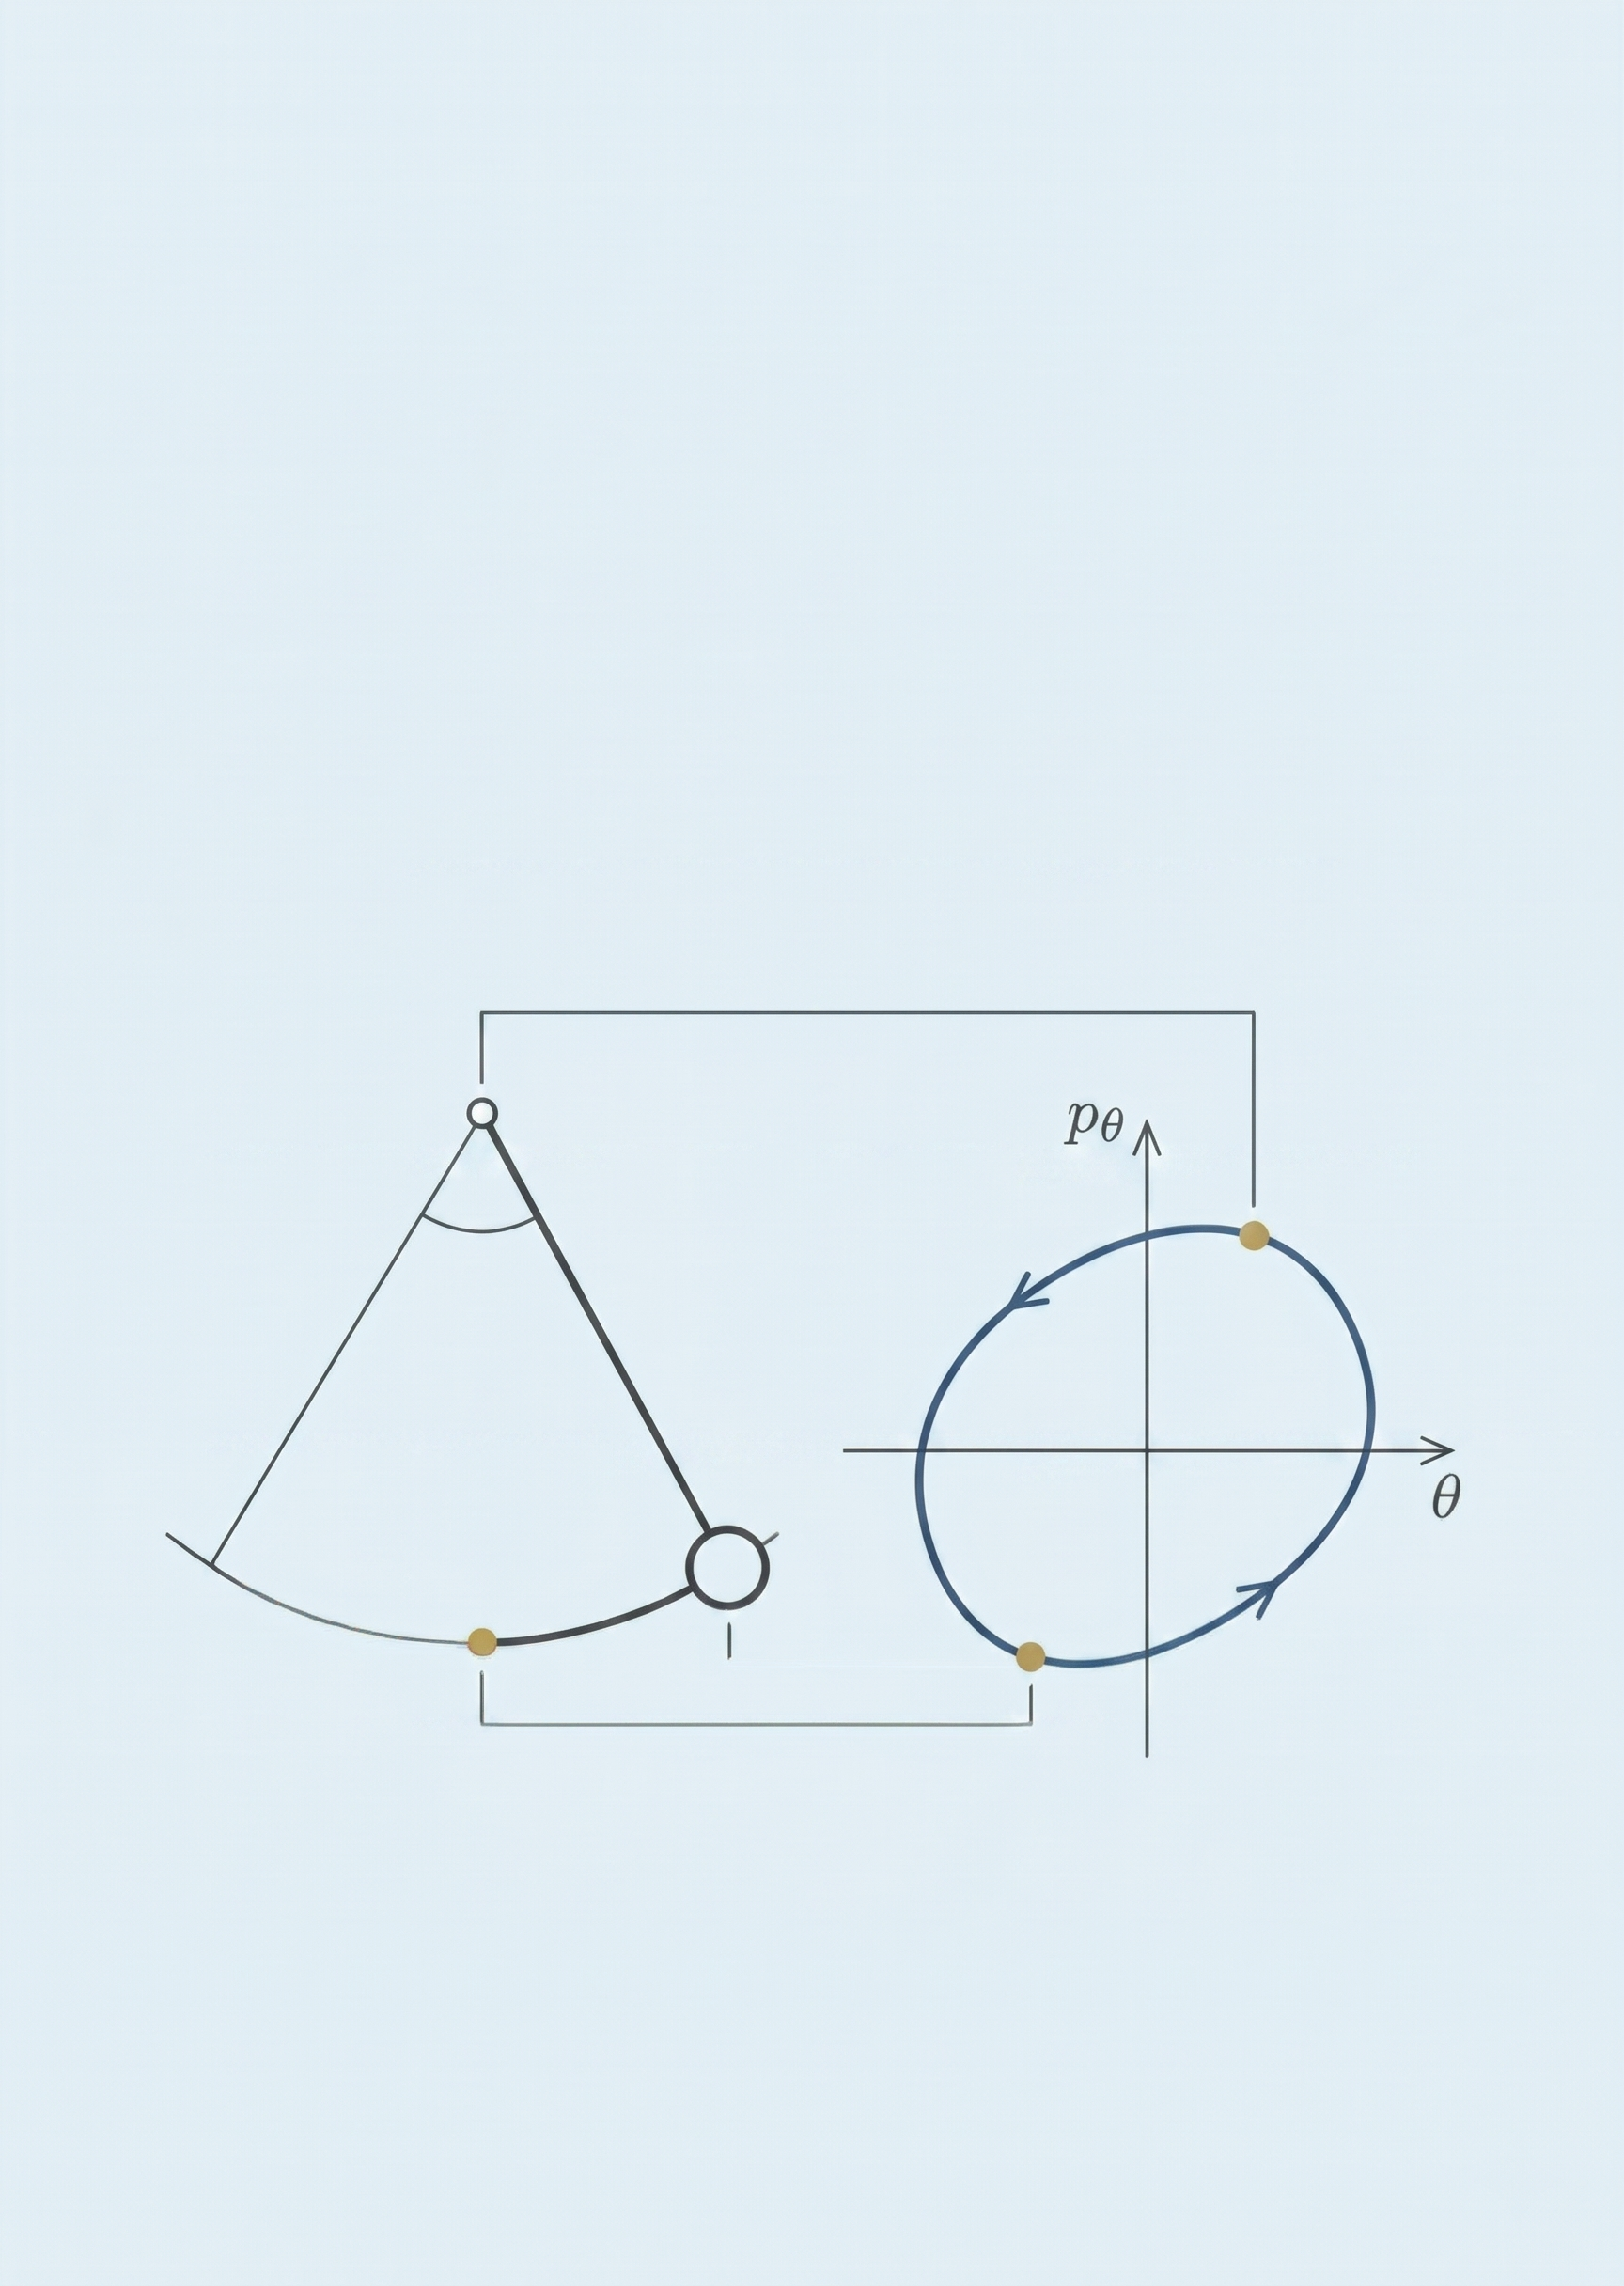
\includegraphics[height=\paperheight,keepaspectratio]{../../../generated_course_notes/core/classical_mechanics/2011_fall_theoretical_minimum/assets/cover-art.png}%
  };
  \node[
    anchor=north west,
    align=left,
    text width=0.78\paperwidth,
    fill=white,
    fill opacity=0.9,
    rounded corners=8pt,
    inner xsep=10pt,
    inner ysep=8pt
  ] at ([xshift=0.08\paperwidth,yshift=-0.06\paperheight]current page.north west) {%
    {\fontsize{30}{33}\selectfont\bfseries\color{black!88} Klassische Mechanik\\[0.85em]}
    {\large\color{black!72} Deutsche Ausgabe / Herbst 2011, Theoretisches Minimum}
  };
  \node[
    anchor=south west,
    align=left,
    text width=0.68\paperwidth,
    fill=white,
    fill opacity=0.82,
    text opacity=1,
    rounded corners=6pt,
    inner sep=12pt
  ] at ([xshift=0.08\paperwidth,yshift=0.08\paperheight]current page.south west) {%
    {\normalsize\color{black!78} Originalvorlesungen: Leonard Susskind\\[0.35em]}
    {\small\color{black!72} Begleitausgabe: \href{https://lazying.art}{LazyingArt LLC} / \href{https://github.com/lachlanchen/Video2Book}{Video2Book}}
  };
\end{tikzpicture}
\mbox{}
\end{titlepage}
\hypersetup{pageanchor=true}

\clearpage
\chapter*{Zu diesen Notizen}
Diese unabhängig redigierten Begleitnotizen folgen den Vorlesungen von Leonard Susskind. Sie wurden anhand maschineller Transkripte, Untertitel und ausgewählter Tafelbilder rekonstruiert und anschließend mit dem verfügbaren Quellenmaterial abgeglichen. Sie sind kein Originalmanuskript von Professor Susskind und wurden von ihm weder geprüft noch autorisiert.

Diese Ausgabe wurde von \href{https://lazying.art}{LazyingArt LLC} mithilfe des Open-Source-\href{https://github.com/lachlanchen/Video2Book}{Video2Book}-Workflows erstellt. Maschinelle Transkripte sind separat verfügbar und können Erkennungsfehler enthalten. Redaktionelle Klarstellungen und wesentliche Rekonstruktionen sind in Fußnoten gekennzeichnet.
\clearpage
\tableofcontents
\mainmatter
\chapter{Zustände, Umkehrbarkeit und Kinematik}

Die klassische Mechanik ist nicht bloß eine Sammlung von Gleichungen für fallende Körper, umlaufende Planeten oder geladene Teilchen. Bevor wir eine bestimmte Gleichung auswählen, können wir eine allgemeinere Frage stellen: Wie muss ein Bewegungsgesetz aussehen, damit es als klassisches Gesetz gelten kann? Wir beginnen mit so einfachen Systemen, dass sich jeder mögliche Verlauf an der Tafel darstellen lässt. Wenn dort die Begriffe Zustand, Determinismus, Umkehrbarkeit und Erhaltung klar geworden sind, kehren wir zu Teilchen zurück, die sich im gewöhnlichen Raum bewegen.

\section{Zwei Arten von Fragen}

In der Mechanik gibt es zwei Arten von Fragen. Die eine fragt nach dem konkreten Gesetz, das ein bestimmtes System beherrscht. Ein Planet, der sich im Gravitationsfeld eines massereichen Körpers bewegt, folgt einem Gesetz; ein elektrisch geladenes Teilchen, das sich in einem Magnetfeld bewegt, einem anderen. Dabei geht es um die detaillierten Naturgesetze.

Die andere Frage betrifft den Rahmen, der all diesen Beispielen gemeinsam ist. Gibt es Regeln, die jedes zulässige Gesetz erfüllen muss? Welche Merkmale gehören zur klassischen Mechanik selbst, unabhängig von der Kraft oder dem untersuchten Objekt? Die konkreten Beispiele werden die Antwort veranschaulichen, doch dieses zweite Problem gibt dem Fach seine Struktur.

Das nützlichste erste Beispiel ist eine abstrakte Münze auf einem abstrakten Tisch. Wir behalten von der Münze nur eine Eigenschaft bei: Sie kann Kopf oder Zahl zeigen. Ihr Konfigurationsraum ist daher \begin{equation}
  \mathcal C=\{H,T\}.
\end{equation}Das Wort \emph{Konfiguration} bezeichnet eine der möglichen Beschaffenheiten des Systems. Eine Anfangsbedingung ist die Wahl einer davon. Eine Münze mit nur einer Seite wäre noch einfacher, hätte aber nur eine Konfiguration, sodass nichts geschehen könnte. Zwei Zustände genügen, um Dynamik zu ermöglichen.

\section{Die Münze: Zustand, Gesetz und Verlauf}

Die Zeit schreitet in ganzzahligen Schritten voran, als würde die Welt mit einem Stroboskop beleuchtet: \begin{equation}
  t=\ldots,-2,-1,0,1,2,\ldots .
\end{equation}Ein Bewegungsgesetz ist eine Aktualisierungsregel. Es ordnet dem Zustand zur Zeit \(t\) einen Zustand zur Zeit \(t+1\) zu. Die einfachste Regel lässt alles unverändert: \begin{equation}
  H\longmapsto H,
  \qquad
  T\longmapsto T.
  \label{eq:coin-identity}
\end{equation}Ausgehend von \(H\) ist der gesamte Verlauf \(H,H,H,\ldots\); ausgehend von \(T\) ist er \(T,T,T,\ldots\). Die Regel ist langweilig, aber sie erlaubt vollständige Vorhersagen.

Die andere umkehrbare Regel vertauscht die beiden Zustände: \begin{equation}
  H\longmapsto T,
  \qquad
  T\longmapsto H.
  \label{eq:coin-flip}
\end{equation}Die Verläufe wechseln nun ab: \begin{equation}
  H,T,H,T,\ldots,
  \qquad
  T,H,T,H,\ldots .
\end{equation}Ein Pfeil zeigt vom Zustand vor der Aktualisierung zum Zustand danach. Das Ende des Pfeils gibt also an, wo das System beginnt, die Pfeilspitze, wohin es gelangt.

\begin{figure}[htbp]\centering
  \includegraphics[width=0.86\textwidth]{lecture_01_figure_02.png}\caption{Die beiden Konfigurationen der Münze und das gerichtete Wurfgesetz an der Vorlesungstafel. Die übersichtliche Aktualisierungsregel steht in Gl.~\eqref{eq:coin-flip}}\lectureframe{00:06:50}\label{fig:coin-board}\end{figure}

Die Seiten lassen sich durch eine Variable mit zwei möglichen Werten kodieren: \begin{equation}
  \sigma=
  \begin{cases}
    +1,&H,\\
    -1,&T.
  \end{cases}
\end{equation}Der Buchstabe \(\sigma\) wird in der Physik traditionell für Größen mit zwei möglichen Werten verwendet, insbesondere bei Beschreibungen des Spins; Kenntnisse über Spin sind hier jedoch nicht erforderlich. Mit dieser Notation werden die beiden Regeln zu Bewegungsgleichungen: \begin{align}
  \sigma(t+1)&=\sigma(t),
  &&\text{identity law},\label{eq:sigma-identity}\\
  \sigma(t+1)&=-\sigma(t),
  &&\text{flip law}.\label{eq:sigma-flip}
\end{align}Die Variable fügt keine neue Physik hinzu. Sie liefert eine kompakte Bezeichnung für die Konfiguration und macht aus einem Graphen eine Gleichung.

\begin{figure}[htbp]\centering
  \includegraphics[width=0.86\textwidth]{lecture_01_figure_03.png}\caption{Das Wurfgesetz in der Form \(\sigma(t+1)=-\sigma(t)\). Die eingerahmten Werte \(\sigma=\pm1\) bezeichnen Kopf und Zahl.}\lectureframe{00:08:58}\label{fig:sigma-board}\end{figure}

Bei beiden Regeln bestimmen der Anfangszustand und das Gesetz den Zustand zu jedem späteren Zeitpunkt. Diese Aussage setzt voraus, dass das System \emph{abgeschlossen} ist. Greift jemand ein und dreht die Münze um, dann ist die Hand ein äußerer Einfluss, der in unserer Beschreibung nicht berücksichtigt wird. Damit haben wir den Determinismus nicht widerlegt, sondern das System geändert. Ein klassisches Gesetz soll ein abgeschlossenes System beherrschen, in dessen Beschreibung alle für seine Entwicklung relevanten Einflüsse enthalten sind.

Es gibt vier mathematische Funktionen von einer zweielementigen Menge in sich selbst. Die beiden oben nicht angegebenen schicken beide Eingaben auf \(H\) beziehungsweise beide auf \(T\). Sie sind für die Zukunft deterministisch, tilgen aber die Unterscheidung zwischen zwei möglichen Vergangenheiten. Wenn wir im Folgenden Umkehrbarkeit fordern, sind die Gl.~\eqref{eq:coin-identity} und \eqref{eq:coin-flip} genau die beiden zulässigen Abbildungen.

\section{Ein Würfel: Bahnen und Erhaltungsgrößen}

Ersetzen wir die Münze durch einen Würfel. Für unsere Zwecke ist an einem Würfel nur wichtig, dass er sechs Konfigurationen hat: \begin{equation}
  \mathcal C=\{1,2,3,4,5,6\}.
\end{equation}Eine Anfangsbedingung ist die Wahl einer Zahl. Wir könnten wiederum jeden Zustand unverändert lassen, doch gerichtete Graphen sind für weniger triviale Regeln nützlicher. Betrachten wir \begin{equation}
  1\longmapsto2\longmapsto3\longmapsto4
  \longmapsto5\longmapsto6\longmapsto1.
  \label{eq:six-cycle}
\end{equation}Ausgehend von \(4\) lautet der Verlauf beispielsweise

\[
  4,5,6,1,2,3,4,\ldots .
\]\footnote{Quelle: Beim ersten mündlichen Durchgehen der Pfeile heißt es an einer Stelle, \(6\) kehre zu \(6\) zurück. Die unmittelbar folgende Formulierung, der gezeichnete Zyklus und der aufgezählte Verlauf geben alle die beabsichtigte Aktualisierung \(6\mapsto1\) wieder.}

\begin{figure}[htbp]\centering
  \includegraphics[width=0.86\textwidth]{lecture_01_figure_06.png}\caption{Der einzelne Zyklus mit sechs Zuständen. Bei jedem Stroboskopschritt geht ein Zustand in den nächsten über; nach sechs Aktualisierungen kehrt er zum Ausgangszustand zurück.}\lectureframe{00:12:40}\label{fig:six-cycle-board}\end{figure}

Ein Gesetz kann komplizierter aussehen, ohne sich strukturell zu unterscheiden. Zum Beispiel ist \begin{equation}
  1\to2\to5\to3\to4\to6\to1
  \label{eq:relabeled-cycle}
\end{equation} weiterhin ein einzelner Zyklus mit sechs Zuständen. Ordnet man die Knoten auf der Seite in der Reihenfolge \(1,2,5,3,4,6\) an, ergibt sich dasselbe Bild wie in Gl.~\eqref{eq:six-cycle}. Bezeichnungen wie \(1\) und \(5\) sind Namen; die Zyklusstruktur hängt nicht von ihnen ab.

Ein tatsächlich anderes Gesetz teilt die sechs Zustände in zwei Zyklen auf, zum Beispiel \begin{equation}
  1\to2\to3\to1,
  \qquad
  4\to6\to5\to4.
  \label{eq:two-cycles}
\end{equation}Es gibt weiterhin einen Würfel und ein Gesetz, aber eine Bahn, die auf einem Zyklus beginnt, kann den anderen niemals erreichen. Wir können den Zyklen eine Zahl \(Q\) zuordnen: \begin{equation}
  Q=
  \begin{cases}
    0,&\text{on the cycle }\{1,2,3\},\\
    1,&\text{on the cycle }\{4,5,6\}.
  \end{cases}
\end{equation}Der Zustand ändert sich bei jedem Schritt, während \(Q\) unverändert bleibt.

\begin{definition}Eine Erhaltungsgröße ist eine Funktion des Zustands, deren Wert sich unter dem Bewegungsgesetz nicht ändert.\end{definition}

Dieselbe Idee ermöglicht einen Fixpunkt, einen Zweierzyklus und einen Dreierzyklus. Die erhaltene Kennzeichnung gibt an, auf welcher Bahn sich das System befindet; den Zustand innerhalb dieser Bahn muss sie nicht bestimmen. Erhaltung ist somit mit Bewegung vereinbar. Erhalten bleibt nicht unbedingt die vollständige Konfiguration, sondern möglicherweise nur eine Unterscheidung zwischen möglichen Konfigurationen.

\begin{figure}[htbp]\centering
  \includegraphics[width=0.86\textwidth]{lecture_01_figure_07.png}\caption{Mehrere voneinander getrennte Zyklen an der Tafel: ein Fixpunkt, ein Zweierzyklus und ein Dreierzyklus. Die Zykluskennzeichnung bleibt erhalten, auch wenn sich der Zustand auf seinem Zyklus bewegt.}\lectureframe{00:18:40}\label{fig:conserved-cycles-board}\end{figure}

In einem endlichen umkehrbaren System ist jede Bahn ein Zyklus. Ein einzelner Zyklus besitzt keine nichtkonstante Erhaltungsgröße dieser einfachen Art, denn die Bahn durchläuft schließlich jeden Zustand. Mehrere Zyklen erlauben eine solche Kennzeichnung, weil die Entwicklung einen Zustand niemals von einer Komponente in eine andere überführt.

\section{Was muss in einem Zustand enthalten sein?}

Bei den Münzbeispielen hing der nächste Seitenwurf nur von der aktuellen Seite ab. Eine Frage aus dem Publikum prüft, ob diese Einschränkung wesentlich ist.

\begin{classroomqa}\audiencequestion{Lässt sich eine Folge von Kopf und Zahl konstruieren, bei der das nächste Ergebnis von mehr als der unmittelbar sichtbaren Seite abhängt, vielleicht von einem oder mehreren früheren Ergebnissen?\lecturetimestamp{00:19:27--00:21:23}}

\lecturerresponse{Ja. In diesem Fall ist weder \(H\) noch \(T\) für sich genommen der vollständige Zustand. Wird eine frühere Seite benötigt, erweitern wir den Zustandsraum zu \(
  \{HH,HT,TH,TT\}.
\)Jedes geordnete Paar hält die aktuelle und die vorhergehende Seite fest. Die Entwicklung lässt sich dann wieder als Einschrittregel auf diesem vier Zustände umfassenden Raum schreiben. Wird noch mehr Verlauf benötigt, nehmen wir auch diese Information auf.}\end{classroomqa}

Diese Antwort gibt dem Zustand seine operationale Bedeutung.

\begin{definition}Der Zustand eines Systems zu einem bestimmten Zeitpunkt umfasst alle Informationen, die zusammen mit dem Bewegungsgesetz benötigt werden, um seine Zukunft vorherzusagen.\end{definition}

Ein Zustand ist also nicht bloß eine Momentaufnahme. Gemeint ist die vollständige Menge an Daten, die die Entwicklung eindeutig festlegt. Später wird die Position allein nicht ausreichen, wenn wir ein Newtonsches Teilchen beschreiben; auch die Geschwindigkeit gehört zu den Anfangsdaten. Die Münze mit Gedächtnis ist die einfachste Ausprägung desselben Prinzips.

\section{Unendliche Zustandsräume}

Unendlich viele Zustände erfordern nicht unendlich viele Objekte. Betrachten wir ein Teilchen, das auf die ganzzahligen Punkte einer unendlichen Geraden beschränkt ist. Sein Zustand ist eine ganze Zahl: \[
  n\in\mathbb Z.
\]Ein Gesetz bewegt es bei jedem Schritt um einen Punkt nach rechts: \begin{equation}
  n(t+1)=n(t)+1.
  \label{eq:lattice-one}
\end{equation}Diese Bahn schließt sich nie, durchläuft aber jede ganze Zahl, wenn man sie sowohl in die Zukunft als auch in die Vergangenheit verfolgt. In diesem erweiterten Sinn spielt sie die Rolle eines einzigen endlosen Zyklus.

Ein anderes Gesetz verschiebt das Teilchen bei jedem Schritt um zwei Punkte: \begin{equation}
  n(t+1)=n(t)+2.
  \label{eq:lattice-two}
\end{equation}Nun entwickelt sich jeder gerade Zustand ausschließlich über gerade Zustände und jeder ungerade ausschließlich über ungerade Zustände. Die Parität bleibt erhalten: \begin{equation}
  \begin{aligned}
    Q_{\rm parity}(n)&=n\bmod 2,\\
    Q_{\rm parity}(n(t+1))&=Q_{\rm parity}(n(t)).
  \end{aligned}
\end{equation}Der Übergang von einem endlichen zu einem unendlichen Konfigurationsraum erlaubt Verläufe, die sich nie wiederholen, ändert aber nichts an der Bedeutung von Zustand, Bahn oder Erhaltung.

\section{Determinismus bedeutet noch keine Umkehrbarkeit}

Nun zeichnen wir eine Regel, die die Zukunft eindeutig vorhersagt, aber eine zweite klassische Forderung nicht erfüllt. Geben wir einer dreiseitigen Münze die Zustände Kopf, Zahl und Kante und legen wir fest: \begin{equation}
  H\to T,
  \qquad
  T\to E,
  \qquad
  E\to T.
  \label{eq:nonreversible-map}
\end{equation}Ausgehend von \(H\) lautet der Verlauf \[
  H,T,E,T,E,\ldots;
\]; beginnt man dagegen mit \(T\) oder \(E\), ist der anschließende Wechsel ebenso eindeutig. Von jedem Zustand geht genau ein Pfeil aus, also ist die Regel für die Zukunft deterministisch.

Das Problem zeigt sich, wenn wir versuchen, die Vergangenheit zu rekonstruieren. Ist der aktuelle Zustand \(T\), könnte der vorhergehende Zustand entweder \(H\) oder \(E\) gewesen sein. Zwei Verläufe sind zusammengeführt worden. Kehrt man alle Pfeile um, wird der Mangel unmittelbar sichtbar: Von \(T\) aus bietet der umgekehrte Graph zwei mögliche Schritte. Die umgekehrte Regel ist nicht deterministisch.

\begin{figure}[htbp]\centering
  \includegraphics[width=0.86\textwidth]{lecture_01_figure_08.png}\caption{Das nichtumkehrbare Gesetz \(H,T,E\) und beispielhafte Verläufe. Sowohl \(H\) als auch \(E\) führen zu \(T\), daher bestimmt die Gegenwart keine eindeutige Vergangenheit.}\lectureframe{00:28:50}\label{fig:nonreversible-board}\end{figure}

\begin{definition}Ein diskretes Gesetz ist umkehrbar, wenn der aktuelle Zustand sowohl den nächsten als auch den vorhergehenden Zustand eindeutig festlegt. Im Zustandsgraphen muss von jedem Zustand genau ein Pfeil ausgehen und genau ein Pfeil in ihn hineinführen.\end{definition}

Für einen endlichen Zustandsraum ist eine umkehrbare Aktualisierung eine Permutation der Zustände. Sie erzeugt oder beseitigt keine Unterscheidungen zwischen Zuständen, sondern ordnet sie lediglich neu an. Deshalb zerfällt ihr Graph in Zyklen. Die Abbildung in Gl.~\eqref{eq:nonreversible-map} ist zwar eine Funktion, aber keine injektive Funktion und besitzt daher keine Umkehrabbildung.

\begin{classroomqa}\audiencequestion{Wäre eine Regel dieser Art zulässig, wenn die Zustände Wahrscheinlichkeiten für ein Teilchen darstellten?\lecturetimestamp{00:29:46--00:31:17}}

\lecturerresponse{Das wäre ein anderer Rahmen. Die grundlegende klassische Mechanik, wie wir sie hier formulieren, verwendet deterministische Gesetze statt probabilistischer Aktualisierungsregeln. Man kann eine solche Regel durchaus erfinden und untersuchen, aber in diesem Sinne ist sie kein klassisches mechanisches Gesetz. Die Quantenmechanik ist nicht auf dieselbe Weise deterministisch und besitzt dennoch ein Analogon umkehrbarer Entwicklung; das erfordert eine spätere Diskussion. Auch die klassische statistische Mechanik verwendet Wahrscheinlichkeiten, geht aber von zugrunde liegenden mechanischen Gesetzen aus und beschreibt damit unvollständige Kenntnis der Anfangsdaten.}\end{classroomqa}

Diese Unterscheidung ist wichtig. Eine Wahrscheinlichkeitsverteilung, die wir verwenden, weil wir den genauen klassischen Zustand nicht kennen, ist kein indeterministisches Bewegungsgesetz. Sie beschreibt unseren Kenntnisstand über ein System, dessen mikroskopische Entwicklung weiterhin als deterministisch und umkehrbar gilt.

\section{Exakte Gesetze und unvollständige Kenntnis}

Für eine Vorhersage sind zwei Zutaten erforderlich: \begin{enumerate}\item das Bewegungsgesetz; \item der Anfangszustand.\end{enumerate}Ein exaktes Gesetz führt nicht zu einer exakten Vorhersage, wenn die Anfangsbedingung nur näherungsweise bekannt ist. Bei der Münze lässt sich leicht vorstellen, dass man auf den Tisch schaut und die Seite einwandfrei erkennt. Reale mechanische Variablen sind kontinuierlich. Positionen und Geschwindigkeiten können beliebige reelle Werte annehmen, und keine Messung liefert unendlich viele Dezimalstellen.

Nehmen wir an, der tatsächliche Anfangszustand liege in einem kleinen Bereich möglicher Zustände. Bei manchen Dynamiken bleibt dieser Bereich lange klein; bei anderen entfernen sich benachbarte Anfangszustände rasch voneinander. In einem chaotischen System wachsen kleine Unsicherheiten im Anfangszustand schließlich zu großen Abweichungen an. Die Atmosphäre ist ein vertrautes Beispiel. Genauere Messungen können den Zeitraum verlängern, für den die Vorhersage brauchbar bleibt. Doch bei jeder festgelegten Messgenauigkeit gibt es einen ausreichend weit entfernten Zeitpunkt, ab dem die Vorhersage unzuverlässig wird.

Diese praktische Einschränkung führt keine Mehrdeutigkeit in die Gleichungen ein. Wären die Anfangsbedingungen exakt bekannt, würde ein klassisches umkehrbares Gesetz sowohl die Zukunft als auch die Vergangenheit festlegen. Bei endlicher Genauigkeit lautet die quantitative Frage vielmehr: Wie genau muss der Anfangszustand bekannt sein, damit eine Vorhersage für einen vorgegebenen Zeitraum möglich ist?

Der graphische Test führt nun zu einer knappen Schlussfolgerung. Ein Gesetz, bei dem an jedem Zustand genau ein Pfeil eintrifft und genau einer ausgeht, ist deterministisch und umkehrbar. Die entsprechenden Aussagen für Teilchen sind weniger elementar, drücken aber dieselbe klassische Struktur aus.

\section{Von abstrakten Zuständen zu Punkten im Raum}

Nun wenden wir uns von Münzen und Würfeln den Punktteilchen zu. Ein Teilchen kann sich in einer, drei, fünf oder beliebig vielen Dimensionen bewegen; der gewöhnliche Raum liefert jedoch das naheliegende Beispiel. Um einen Punkt quantitativ zu beschreiben, wählen wir: \begin{itemize}\item einen Ursprung; \item drei zueinander senkrechte Achsen; \item eine Orientierung dieser Achsen; \item eine Längeneinheit.\end{itemize}Die Wahl des Ursprungs ist Konvention. Er kann in Palo Alto oder anderswo liegen, und physikalische Schlussfolgerungen sollten nicht von dieser Wahl abhängen. Die Achsen können mit \(x,y,z\) oder \(x_1,x_2,x_3\) beschriftet werden. Nachdem die \(x\)- und \(y\)-Richtungen festgelegt sind, kann die \(z\)-Achse in eine von zwei zueinander senkrechten Richtungen zeigen. Wir wählen die Rechtshandkonvention: Zeigt der Daumen der rechten Hand entlang \(x\) und der Zeigefinger entlang \(y\), so weist der Mittelfinger entlang \(z\).

Gleiche Markierungen auf den Achsen erfordern eine Einheit, etwa Meter, Fuß, Zoll oder Lichtjahre. Sind diese Konventionen festgelegt, wird jeder Punkt durch drei Zahlen bezeichnet: \begin{equation}
  (x,y,z).
\end{equation}Vom Ursprung aus lässt sich der Punkt durch Verschiebungen entlang der drei Achsen erreichen. Für ein System aus vielen Teilchen benötigt man je Teilchen ein solches Zahlentripel.

\begin{figure}[htbp]\centering
  \includegraphics[width=0.86\textwidth]{lecture_01_figure_09.png}\caption{Kartesische Achsen und die drei Koordinaten eines Punktes. Die Zeichnung legt eine Koordinatenkonvention fest; der Punkt selbst hängt nicht davon ab, wo wir Ursprung oder Achsen wählen.}\lectureframe{00:43:00}\label{fig:coordinates-board}\end{figure}

\section{Vektoren und ihre Komponenten}

Ein Vektor ist ein Objekt mit Betrag und Richtung. Die Verschiebung vom Ursprung zu einem Punkt ist ein Vektor; Vektoren beschreiben aber auch Geschwindigkeit, Beschleunigung, elektrische Felder und viele weitere Größen. Einen Vektor schreiben wir fett, zum Beispiel \(\mathbf v\), seinen Betrag als \(\lvert\mathbf v\rvert\). Der Betrag ist nichtnegativ und nur beim Nullvektor gleich null.

Geometrisch ist ein Vektor ein freier Pfeil. Wird der Pfeil verschoben, ohne seine Länge oder Richtung zu ändern, so bleibt der Vektor derselbe. In einer konkreten Anwendung kann ein Vektor einem Punkt zugeordnet sein, etwa wenn wir das elektrische Feld an einem bestimmten Ort angeben. Diese Zuordnung ist jedoch eine zusätzliche Information und gehört nicht zum abstrakten Vektor selbst.

Bezüglich kartesischer Achsen hat ein Vektor die Komponenten \begin{equation}
  \mathbf v=(v_x,v_y,v_z).
\end{equation}Die Komponenten sind gewöhnliche vorzeichenbehaftete Zahlen, die man durch Projektion auf die Achsen erhält. Sie kodieren Betrag und Richtung. Der Satz des Pythagoras in drei Dimensionen ergibt \begin{equation}
  \lvert\mathbf v\rvert^2
  =v_x^2+v_y^2+v_z^2,
  \qquad
  \lvert\mathbf v\rvert
  =\sqrt{v_x^2+v_y^2+v_z^2}.
  \label{eq:vector-magnitude}
\end{equation}Die Verhältnisse der Komponenten bestimmen die Richtung. Eine negative Komponente bedeutet, dass der Vektor teilweise in Richtung der negativen Achsenrichtung zeigt.

\subsection{Skalarmultiplikation und Addition}

Die Multiplikation mit einer reellen Zahl ändert die Länge eines Vektors und kehrt bei einem negativen Faktor seine Richtung um. Für \(c>0\) zeigt \(c\mathbf A\) in Richtung von \(\mathbf A\) und hat den Betrag \(c\lvert\mathbf A\rvert\). Insbesondere hat \(-\mathbf A\) dieselbe Länge wie \(\mathbf A\) und zeigt in die entgegengesetzte Richtung.

Die Vektoraddition lässt sich auf drei gleichwertige Arten veranschaulichen. Erstens setzt man den Anfang von \(\mathbf B\) an die Spitze von \(\mathbf A\); der Pfeil vom Anfang von \(\mathbf A\) zur Spitze von \(\mathbf B\) ist dann \(\mathbf A+\mathbf B\). Zweitens setzt man beide Pfeilanfänge an denselben Punkt und ergänzt ein Parallelogramm; dessen Diagonale ist die Summe. An dieser Darstellung wird die Kommutativität sichtbar: \begin{equation}
  \mathbf A+\mathbf B=\mathbf B+\mathbf A.
\end{equation}Drittens addiert man die entsprechenden Komponenten: \begin{equation}
  C_i=A_i+B_i,
  \qquad i=x,y,z,
  \label{eq:component-addition}
\end{equation}wobei \(\mathbf C=\mathbf A+\mathbf B\) gilt. Mit diesen Regeln lassen sich auch beliebige Linearkombinationen wie \(a\mathbf A+b\mathbf B\) bilden.

\begin{figure}[htbp]\centering
  \includegraphics[width=0.86\textwidth]{lecture_01_figure_10.png}\caption{Dreiecks- und Parallelogrammkonstruktion für die Vektoraddition. Beide ergeben denselben Vektor \(\mathbf A+\mathbf B\).}\lectureframe{00:53:00}\label{fig:vector-addition-board}\end{figure}

Eine allgemeine Möglichkeit, einen Vektor durch einen anderen zu dividieren, gibt es nicht. Es gibt jedoch zwei übliche Vektorprodukte. Das Kreuzprodukt behandeln wir in einer späteren Vorlesung. Hier benötigen wir das Skalarprodukt.

\subsection{Das Skalarprodukt}

Projizieren wir \(\mathbf A\) auf die von \(\mathbf B\) bestimmte Achse. Beträgt der Winkel zwischen den Vektoren \(\theta\), so ist die vorzeichenbehaftete Komponente von \(\mathbf A\) in Richtung von \(\mathbf B\) gleich \(\lvert\mathbf A\rvert\cos\theta\). Multiplizieren wir diese Projektion mit \(\lvert\mathbf B\rvert\), erhalten wir die Definition von \begin{equation}
  \mathbf A\cdot\mathbf B
  =\lvert\mathbf A\rvert\,\lvert\mathbf B\rvert\cos\theta.
  \label{eq:dot-geometric}
\end{equation}Das Ergebnis ist ein Skalar, kein weiterer Vektor. Gl.~\eqref{eq:dot-geometric} ist symmetrisch in \(\mathbf A\) und \(\mathbf B\), also gilt \(\mathbf A\cdot\mathbf B=\mathbf B\cdot\mathbf A\).

\begin{figure}[htbp]\centering
  \includegraphics[width=0.86\textwidth]{lecture_01_figure_11.png}\caption{Geometrische Herleitung des Skalarprodukts durch Projektion an der Tafel. Die gesetzte Form lautet \(\mathbf A\cdot\mathbf B=AB\cos\theta\).}\lectureframe{00:58:30}\label{fig:dot-product-board}\end{figure}

Das Vorzeichen enthält geometrische Information. Bei einem spitzen Winkel ist das Skalarprodukt positiv, bei einem stumpfen negativ und bei senkrechten Vektoren null. Daher gilt \begin{equation}
  \mathbf A\perp\mathbf B
  \quad\Longleftrightarrow\quad
  \mathbf A\cdot\mathbf B=0
\end{equation}für von null verschiedene Vektoren.

In Komponenten lautet das Skalarprodukt \begin{equation}
  \mathbf A\cdot\mathbf B
  =A_xB_x+A_yB_y+A_zB_z.
  \label{eq:dot-components}
\end{equation}Diese Formel macht Berechnungen unmittelbar. Insbesondere gilt \begin{equation}
  \mathbf A\cdot\mathbf A
  =A_x^2+A_y^2+A_z^2
  =\lvert\mathbf A\rvert^2.
  \label{eq:self-dot}
\end{equation}Aus den Komponenten zweier Vektoren bestimmen die Gl.~\eqref{eq:dot-geometric} und \eqref{eq:dot-components} den Winkel zwischen ihnen: \begin{equation}
  \cos\theta
  =\frac{\mathbf A\cdot\mathbf B}
  {\lvert\mathbf A\rvert\,\lvert\mathbf B\rvert}.
\end{equation}

Der Kosinussatz folgt aus derselben Rechnung. Seien \(\mathbf A\) und \(\mathbf B\) die Vektoren von einem gemeinsamen Eckpunkt zu den beiden anderen Eckpunkten eines Dreiecks. Die dritte Seite ist \(\mathbf C=\mathbf A-\mathbf B\), nicht \(\mathbf A+\mathbf B\). Daher gilt \begin{align}
  C^2
  &=(\mathbf A-\mathbf B)\cdot(\mathbf A-\mathbf B)\notag\\
  &=A^2+B^2-2\mathbf A\cdot\mathbf B\notag\\
  &=A^2+B^2-2AB\cos\theta.
  \label{eq:law-of-cosines}
\end{align}

\begin{figure}[htbp]\centering
  \includegraphics[width=0.86\textwidth]{lecture_01_figure_04.png}\caption{Das Dreieck zum Kosinussatz. Die Korrektur an der Tafel identifiziert die schließende Seite als \(\mathbf C=\mathbf A-\mathbf B\); daraus folgt Gl.~\eqref{eq:law-of-cosines}.}\lectureframe{01:04:29}\label{fig:law-cosines-board}\end{figure}

\section{Position, Geschwindigkeit und Beschleunigung}

Wählen wir einen Ursprung und bezeichnen wir mit \(\mathbf r\) den Ortsvektor vom Ursprung zum Teilchen. Seine Komponenten sind die kartesischen Koordinaten: \begin{equation}
  \mathbf r=(x,y,z),
  \qquad
  \lvert\mathbf r\rvert=\sqrt{x^2+y^2+z^2}.
\end{equation}Eine Änderung des Ursprungs verändert \(\mathbf r\); diese Frage vertagen wir. Bei festem Ursprung wird die Bewegung durch einen zeitabhängigen Ort beschrieben: \begin{equation}
  \mathbf r(t)=\bigl(x(t),y(t),z(t)\bigr).
\end{equation}Die Bahn ist somit durch drei Funktionen der Zeit kodiert.

Die Geschwindigkeit ist die zeitliche Ableitung des Ortes: \begin{equation}
  \mathbf v(t)=\frac{d\mathbf r}{dt}
  =\dot{\mathbf r}(t),
  \qquad
  v_i=\frac{dx_i}{dt}=\dot x_i.
  \label{eq:velocity}
\end{equation}Ein Punkt bezeichnet stets eine Ableitung nach der Zeit. Der Betrag \(\lvert\mathbf v\rvert\) ist die Schnelligkeit. Im Allgemeinen sind Ort und Geschwindigkeit voneinander unabhängige Richtungen: Ein Teilchen an einem bestimmten Ort kann sich in jede Richtung bewegen, die das Problem zulässt.

Die Beschleunigung ist die Änderungsrate der Geschwindigkeit und somit die zweite zeitliche Ableitung des Ortes: \begin{equation}
  \mathbf a(t)=\frac{d\mathbf v}{dt}
  =\dot{\mathbf v}(t)
  =\frac{d^2\mathbf r}{dt^2}
  =\ddot{\mathbf r}(t),
  \qquad
  a_i=\ddot x_i.
  \label{eq:acceleration}
\end{equation}Auch die Beschleunigung ist ein Vektor. Wird ein Teilchen, das sich in positiver \(x\)-Richtung bewegt, schneller, so gilt \(a_x>0\). Wird es langsamer, so gilt \(a_x<0\). Was häufig Verzögerung genannt wird, ist einfach eine Beschleunigung entgegen der momentanen Geschwindigkeit. Allgemeiner kann sich die Geschwindigkeit auch dadurch ändern, dass sich ihre Richtung ändert, selbst wenn ihr Betrag konstant bleibt.

\begin{figure}[htbp]\centering
  \includegraphics[width=0.86\textwidth]{lecture_01_figure_05.png}\caption{Geschwindigkeitskomponenten als zeitliche Ableitungen der Ortskomponenten. In kompakter Vektorschreibweise gilt \(\mathbf v=d\mathbf r/dt\).}\lectureframe{01:14:24}\label{fig:velocity-board}\end{figure}

\subsection{Gleichförmige Beschleunigung auf einer Geraden}

Für eine eindimensionale Bewegung schreiben wir \begin{equation}
  x(t)=a+bt+ct^2.
  \label{eq:quadratic-motion}
\end{equation}Bei \(t=0\) befindet sich das Teilchen bei \(x=a\). Einmaliges und anschließendes zweimaliges Differenzieren ergibt \begin{align}
  v(t)=\dot x(t)&=b+2ct,\label{eq:line-velocity}\\
  a(t)=\ddot x(t)&=2c.\label{eq:line-acceleration}
\end{align}Damit ist \(b\) die Anfangsgeschwindigkeit und \(2c\) eine konstante Beschleunigung. Für \(c>0\) steigt die Geschwindigkeit linear; für \(c<0\) sinkt sie linear. Diese quadratische Ortsfunktion beschreibt die Bewegung bei konstanter Beschleunigung, etwa die idealisierte Bewegung eines fallenden Körpers nahe der Erdoberfläche.

\section{Gleichförmige Kreisbewegung}

Als letztes Beispiel betrachten wir ein Teilchen, das sich in der \(x\)-\(y\)-Ebene auf dem Einheitskreis bewegt. Es startet bei \(t=0\) auf der positiven \(x\)-Achse, und seine Winkelkoordinate nimmt gleichmäßig zu: \begin{equation}
  \theta(t)=\omega t.
\end{equation}Die Konstante \(\omega\) ist die Kreisfrequenz. Eine volle Umdrehung entspricht einer Winkelzunahme von \(2\pi\); daher ist die Periodendauer \begin{equation}
  T=\frac{2\pi}{\omega}.
  \label{eq:circular-period}
\end{equation}Der Winkel darf über \(2\pi\) hinaus anwachsen; die Position wiederholt sich, obwohl der fortlaufend erfasste Winkel nicht auf null zurückgesetzt wird.

Auf dem Einheitskreis gilt \begin{equation}
  \mathbf r(t)
  =\bigl(\cos\omega t,\,\sin\omega t\bigr).
  \label{eq:circular-position}
\end{equation}Differenzieren ergibt \begin{equation}
  \mathbf v(t)
  =\omega\bigl(-\sin\omega t,\,\cos\omega t\bigr).
  \label{eq:circular-velocity}
\end{equation}Die Geschwindigkeit ist tangential zum Kreis. Ihre Senkrechtstellung zum Radius lässt sich ohne Rückgriff auf die Zeichnung beweisen: \begin{align}
  \mathbf r\cdot\mathbf v
  &=\cos\omega t\,(-\omega\sin\omega t)
    +\sin\omega t\,(\omega\cos\omega t)\notag\\
  &=0.
  \label{eq:r-dot-v}
\end{align}

\begin{figure}[htbp]\centering
  \includegraphics[width=0.86\textwidth]{lecture_01_figure_12.png}\caption{Orts- und Geschwindigkeitskomponenten für die Bewegung auf dem Einheitskreis. Die Kürzung in \(\mathbf r\cdot\mathbf v\) bestätigt, dass die Geschwindigkeit tangential zum Kreis ist.}\lectureframe{01:24:30}\label{fig:circular-velocity-board}\end{figure}

Nochmaliges Differenzieren ergibt \begin{equation}
  \mathbf a(t)
  =-\omega^2
  \bigl(\cos\omega t,\,\sin\omega t\bigr)
  =-\omega^2\mathbf r(t).
  \label{eq:centripetal-acceleration}
\end{equation}Die Beschleunigung ist parallel zum Radius, zeigt aber in die entgegengesetzte Richtung, also zum Zentrum. Dies ist die Zentripetalbeschleunigung.\footnote{Terminologiehinweis: Das Wort ``Zentrifugal'' fällt an dieser Stelle in der Vorlesung, doch die Gleichung und die begleitende Beschreibung bezeichnen die übliche Zentripetalbeschleunigung, die zum Zentrum gerichtet ist.}

\begin{figure}[H]\centering
  \includegraphics[width=0.86\textwidth]{lecture_01_figure_13.png}\caption{Komponentenrechnung der Kreisbewegungsbeschleunigung. Jede Komponente ist das \(-\omega^2\)-Fache der entsprechenden Ortskomponente, also gilt \(\mathbf a=-\omega^2\mathbf r\).}\lectureframe{01:26:30}\label{fig:circular-acceleration-board}\end{figure}

Da der Radius eins beträgt, gilt \begin{equation}
  \lvert\mathbf r\rvert=1,
  \qquad
  \lvert\mathbf v\rvert=\omega,
  \qquad
  \lvert\mathbf a\rvert=\omega^2.
\end{equation}Eine größere Kreisfrequenz \(\omega\) erhöht die Geschwindigkeit linear und die erforderliche nach innen gerichtete Beschleunigung quadratisch. Für einen Kreis mit Radius \(R\) ergäben dieselbe Rechnung \(v=\omega R\) und \(\lvert\mathbf a\rvert=\omega^2R=v^2/R\); in der Vorlesung wird \(R=1\) verwendet, um die erste Rechnung übersichtlich zu halten.

Damit verfügen wir über die elementaren Begriffe für die Teilchenmechanik: Zustände und Anfangsdaten, umkehrbare Entwicklung, Koordinaten, Vektoren sowie die Ableitungen, die Geschwindigkeit und Beschleunigung definieren. Als Nächstes ist zu klären, welche Anfangsdaten ein Teilchen genau festlegen und welche Gesetze diese Daten von einem Zeitpunkt zum nächsten überführen.
\chapter{Kräfte, Phasenraum und Erhaltungssätze}

\lectureoverview{Ein Bewegungsgesetz muss mehr leisten, als bekannte physikalische Größen miteinander in Beziehung zu setzen. Es muss den Zustand eines Systems angeben, diesen Zustand von einem Zeitpunkt zum nächsten fortschreiben und erkennen lassen, welche Unterscheidungen und Größen die Bewegung überdauern. Wir nähern uns der Newtonschen Mechanik, indem wir zunächst ein plausibles, aber falsches Kraftgesetz prüfen, dann den Zustand von der Position auf den Phasenraum erweitern und schließlich die Erhaltung von Impuls und Energie herleiten.}

\section{Ein nützliches falsches Gesetz}

Die Bewegung im Alltag wird von Reibung beherrscht. Schiebt man einen schweren Gegenstand über den Boden, setzt er sich in Bewegung; hört man auf zu schieben, kommt er bald zum Stillstand. Ein stärkerer Schub führt im Allgemeinen zu einer höheren Geschwindigkeit, während ein schwererer Gegenstand kräftiger geschoben werden muss. In einer solchen Welt liegt die Annahme nahe, dass die Kraft unmittelbar die Geschwindigkeit erzeugt. Dies war die grundlegende Intuition hinter der aristotelischen Beschreibung der Bewegung.

Beim Schlittschuhlaufen macht man die fehlende Erfahrung. Ein Läufer braucht Kraft, um sich in Bewegung zu setzen, anzuhalten oder die Richtung zu ändern, aber nicht, um nach dem Anlaufen weiterzugleiten. Hätte Aristoteles auf nahezu reibungsfreiem Eis statt auf gewöhnlichem Boden gearbeitet, wäre der Fehler in der Kraft--Geschwindigkeit-Intuition viel schwerer zu übersehen gewesen.

Um den Fehler dieser Intuition offenzulegen, geben wir ihr eine präzise moderne Form. Wir schreiben die bewusst falsche Gleichung

\begin{equation}
  \mathbf F=m\mathbf v.
  \label{eq:aristotle-vector-law}
\end{equation}

Dies ist nicht Newtons Gesetz und sollte nicht als Physik auswendig gelernt werden. Ihr Wert liegt darin, dass sie der Diagnose dient: Sobald eine verbale Regel als Gleichung formuliert ist, können wir fragen, ob sie Bewegung vorhersagt und genügend Information bewahrt, um die Vergangenheit zu rekonstruieren. Der kurze Unterrichtsgesprächsbeitrag zum griechischen Wort für Kraft verweist auf \emph{dynamis}, die Wurzel, die auch in Wörtern wie Dynamo und Dynamik anklingt; für die Prüfung des Gesetzes selbst ist die Terminologie jedoch nebensächlich.

\begin{figure}[htbp]\centering
  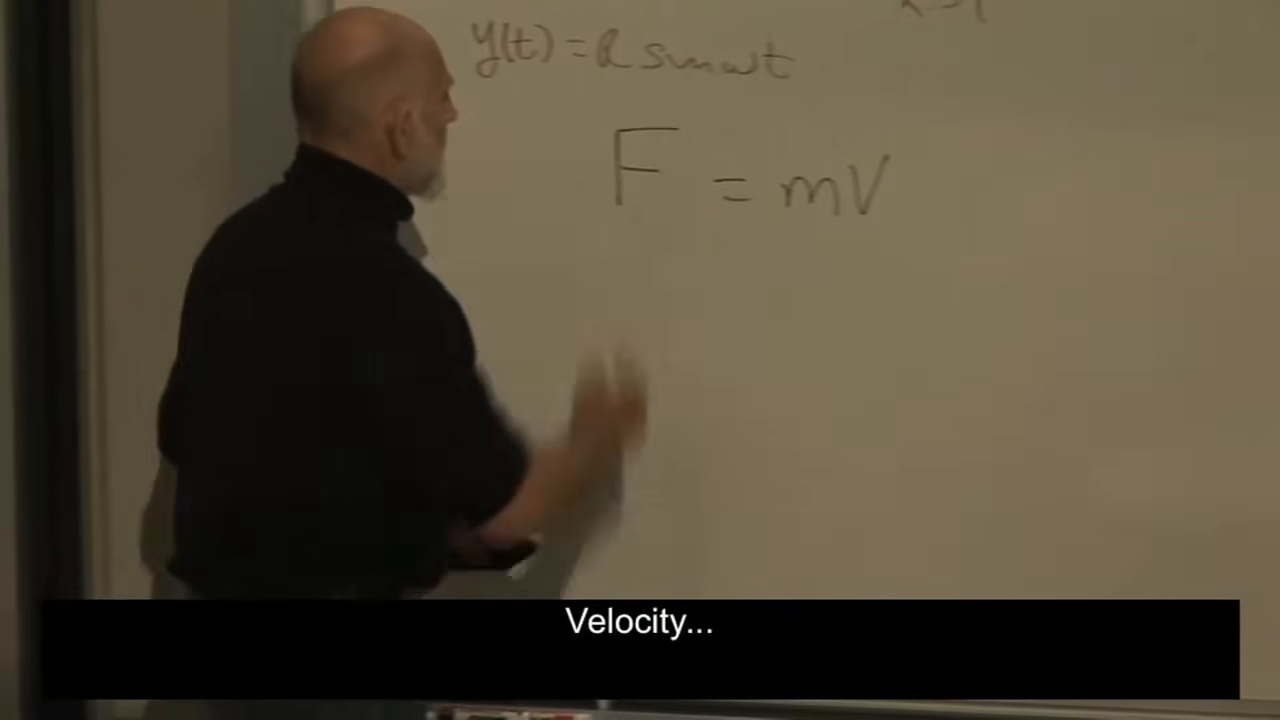
\includegraphics[width=0.82\textwidth]{lecture_02_figure_02.png}\caption{Das absichtlich falsche Kraft--Geschwindigkeit-Gesetz zur Prüfung von Vorhersagbarkeit und Umkehrbarkeit.}\lectureframe{00:04:51}\end{figure}

Beschränken wir die Bewegung auf eine Raumkoordinate. Da \(v=\dot x\) gilt, lautet das Gesetz

\begin{equation}
  F(t)=m\dot x(t).
  \label{eq:aristotle-1d}
\end{equation}

Teilen wir die Zeit nun in kurze Intervalle der Länge \(\delta\) ein. Während eines Intervalls gilt:

\begin{equation}
  \dot x(t)\simeq
  \frac{x(t+\delta)-x(t)}{\delta}.
  \label{eq:first-difference}
\end{equation}

Einsetzen in Gl.~\eqref{eq:aristotle-1d} ergibt

\begin{equation}
  x(t+\delta)
  =x(t)+\frac{\delta}{m}F(t).
  \label{eq:aristotle-update}
\end{equation}

Dies hat die Form einer echten Aktualisierungsregel. Sind die gegenwärtige Position und die Kraft bekannt, folgt daraus die Position zum nächsten stroboskopischen Zeitpunkt. Verschwindet die Kraft, ergibt Aristoteles’ Regel jedoch \(\dot x=0\): Der Gegenstand muss in Ruhe bleiben. Eine Bewegung ohne aufrechterhaltende Kraft ist von Anfang an ausgeschlossen.

\begin{figure}[htbp]\centering
  \includegraphics[width=0.84\textwidth]{lecture_02_figure_07.png}\caption{Die diskrete Aktualisierung nach Aristoteles mit einer rücktreibenden Kraft. Bei jedem Schritt wird die Auslenkung mit einem Faktor multipliziert, der geringfügig kleiner als eins ist.}\lectureframe{00:10:15}\end{figure}

\subsection{Eine Feder in der Mechanik des Aristoteles}

Betrachten wir ein Teilchen, das an einer Feder befestigt ist, deren Gleichgewichtslage bei \(x=0\) liegt. Eine Auslenkung erzeugt die rücktreibende Kraft

\begin{equation}
  F(x)=-kx,
  \qquad k>0.
  \label{eq:hooke-law}
\end{equation}

Setzen wir diese Kraft in Gl.~\eqref{eq:aristotle-update} ein, erhalten wir

\begin{equation}
  x(t+\delta)
  =\left(1-\frac{k\delta}{m}\right)x(t).
  \label{eq:aristotle-spring-update}
\end{equation}

Für hinreichend kleines \(\delta\) liegt der Faktor in der Klammer knapp unter eins. Bei jeder Aktualisierung wird die Auslenkung daher um denselben Anteil verringert:

\begin{equation}
  x_n=\left(1-\frac{k\delta}{m}\right)^n x_0.
  \label{eq:aristotle-geometric-decay}
\end{equation}

Die kontinuierliche Gleichung und ihre Lösung lauten

\begin{align}
  m\dot x&=-kx,
  \label{eq:aristotle-spring-continuous}\\
  x(t)&=x(0)e^{-kt/m}.
  \label{eq:aristotle-spring-solution}
\end{align}

Die Feder führt keine Schwingung aus. Aus jeder Auslenkung freigegeben, nähert sie sich exponentiell dem Ursprung und bewegt sich dabei immer langsamer.

\begin{figure}[htbp]\centering
  \includegraphics[width=0.84\textwidth]{lecture_02_figure_08.png}\caption{Die exponentielle Lösung der aristotelischen Federgleichung. Die Auslenkung klingt ab, statt zu schwingen.}\lectureframe{00:12:02}\end{figure}

Die Zukunft lässt sich leicht vorhersagen: Jede anfängliche Auslenkung nähert sich derselben Ruhelage. Mit der Vergangenheit ist es anders. Angenommen, das Teilchen wird sehr nahe am Ursprung und nur mit endlicher Genauigkeit beobachtet. Es könnte bei einer von vielen verschiedenen Auslenkungen begonnen haben, denn ihre exponentiell kleinen Reste liegen schließlich alle innerhalb derselben Messtoleranz. Bei perfekter mathematischer Genauigkeit lässt sich Gl.~\eqref{eq:aristotle-spring-solution} rückwärts durchlaufen, doch praktische Unterschiede zwischen den Vorgeschichten werden nach und nach ausgelöscht. Vom Standpunkt einer umkehrbaren fundamentalen Dynamik aus ist das Gesetz daher verdächtig.

Das bedeutet nicht, dass Aristoteles irrational war. Die von ihm beschriebene, reibungsdominierte Bewegung ist tatsächlich dissipativ. Der Fehler bestand darin, dieses effektive Verhalten zu einem fundamentalen Gesetz zu erheben. Reibung ist selbst eine Kraft, die aus komplizierten mikroskopischen Wechselwirkungen entsteht. Schiebt eine Hand einen Gegenstand ungefähr mit gleichbleibender Geschwindigkeit, gleicht die ausgeübte Kraft die Reibung aus; sie erzeugt nicht die Geschwindigkeit als solche.

\section{Newtons Gesetz und seine physikalische Bedeutung}

Die Newtonsche Korrektur lautet: Eine Kraft ändert die Bewegung:

\begin{equation}
  \mathbf F=m\mathbf a=m\ddot{\mathbf x}.
  \label{eq:newton-second-law}
\end{equation}

Bevor wir dies als Entwicklungsgleichung auffassen, müssen wir zwei scheinbare Zirkelschlüsse auflösen. Der erste betrifft Bezugssysteme. Oft hört man, Newtons Gesetze gälten in Inertialsystemen und ein Inertialsystem sei eines, in dem Newtons Gesetze gelten. Die physikalische Aussage ist nicht diese zirkuläre Definition. Sie ist die empirische Behauptung, dass \emph{es} Bezugssysteme gibt, die durch geeignete Maßstäbe und Uhren beschrieben werden und in denen Newtons Gesetze ihre einfache Form annehmen. Bezugssysteme, die sich relativ zu ihnen beschleunigen oder drehen, erfordern zusätzliche Scheinkräfte. Wie sich die Gleichungen in diesen anderen Bezugssystemen transformieren, lässt sich später herleiten.

Der zweite Zirkelschluss betrifft Kraft und Masse. Definiert man die Kraft als Masse mal Beschleunigung und die Masse als Kraft geteilt durch Beschleunigung, scheint die Gleichung leer zu sein. Ein operationales Experiment trennt die Definitionen vom Gesetz. Man vergleicht einen Gegenstand mit einem Normkilogramm, indem man beide ins Gleichgewicht bringt, und befestigt den Gegenstand dann in einem ansonsten kraftfreien Raum an einer Federwaage. Eine feste kleine Dehnung der Feder wird als eine Krafteinheit definiert. Zwei identische Federn, die jeweils um denselben Betrag gedehnt werden, liefern zwei Krafteinheiten und erzeugen die doppelte Beschleunigung. Es ist sicherer, eine zweite Feder hinzuzufügen, als eine einzelne Feder doppelt so weit zu dehnen, denn eine reale Feder wird schließlich nichtlinear oder reißt. Lässt man eine Feder unverändert und verbindet sie mit zwei gleichen Massen, beträgt die Beschleunigung die Hälfte; bei drei gleichen Massen beträgt sie ein Drittel.

\begin{figure}[htbp]\centering
  \includegraphics[width=0.84\textwidth]{lecture_02_figure_09.png}\caption{Das Gedankenexperiment mit der Federwaage dient dazu, gleiche Krafteinheiten zu definieren und die Proportionalität der Beschleunigung zur Kraft zu prüfen.}\lectureframe{00:22:45}\end{figure}

Diese Vergleiche verleihen folgender Beziehung empirischen Gehalt:

\begin{equation}
  a\propto F,
  \qquad
  a\propto\frac{1}{m},
  \qquad
  F=ma.
  \label{eq:force-mass-scaling}
\end{equation}

Das Wort \emph{Teilchen} verwenden wir für jeden kleinen Gegenstand, dessen innere Struktur keine Rolle spielt, nicht nur für ein Elementarteilchen.

\subsection{Warum die Position allein kein Zustand ist}

Prüfen wir Newtons Gleichung nun mit derselben stroboskopischen Methode. Der zentrierte Differenzenquotient für die Beschleunigung lautet

\begin{equation}
  \ddot x(t)\simeq
  \frac{x(t+\delta)-2x(t)+x(t-\delta)}{\delta^2}.
  \label{eq:second-difference}
\end{equation}

Daraus folgt aus Newtons Gleichung

\begin{equation}
  x(t+\delta)
  =2x(t)-x(t-\delta)+\frac{\delta^2}{m}F(t).
  \label{eq:newton-position-update}
\end{equation}

Die nächste Position lässt sich nicht allein aus \(x(t)\) bestimmen. Wir benötigen auch die vorherige Position \(x(t-\delta)\) oder gleichbedeutend die Geschwindigkeit zum gegenwärtigen Zeitpunkt. Zunächst scheint Newtons Gleichung dadurch weniger vorhersagekräftig als diejenige von Aristoteles. Die richtige Schlussfolgerung lautet vielmehr, dass die Position allein den Zustand nicht vollständig beschrieb. Alles Relevante zu einem Zeitpunkt zu kennen bedeutet, genügend Daten zu kennen, um die anschließende Bewegung zu bestimmen. Für ein Newtonsches Teilchen sind das Position und Geschwindigkeit.

\section{Impuls und Phasenraum}

Wir führen den Impuls ein durch

\begin{equation}
  \mathbf p=m\mathbf v=m\dot{\mathbf x}.
  \label{eq:momentum-definition}
\end{equation}

Die Masse eines festgelegten Newtonschen Systems wird als konstant angenommen. Ein Gegenstand kann ein Teil verlieren, wie ein Stift seine Kappe, doch dann hat sich der beschriebene Gegenstand geändert; das gewählte abgeschlossene System behält weiterhin seine konstante Gesamtmasse. Bei konstantem \(m\) wird Newtons zweites Gesetz zu

\begin{equation}
  \mathbf F=\dot{\mathbf p}.
  \label{eq:newton-momentum-form}
\end{equation}

\begin{figure}[htbp]\centering
  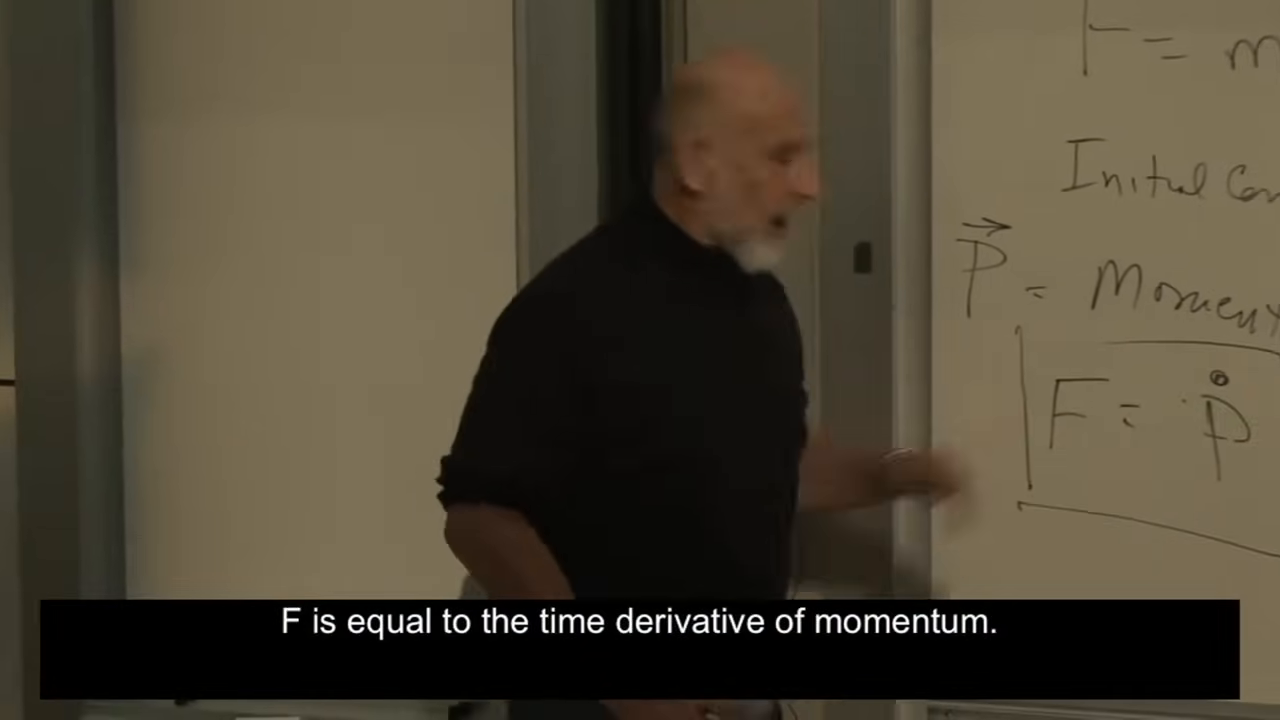
\includegraphics[width=0.82\textwidth]{lecture_02_figure_03.png}\caption{Newtons Gesetz als zeitliche Ableitung des Impulses geschrieben.}\lectureframe{00:32:35}\end{figure}

Für eine Koordinate lässt sich die Newtonsche Bewegung nun durch zwei Differentialgleichungen erster Ordnung für zwei unabhängige Zustandsvariablen beschreiben:

\begin{align}
  \dot p&=F(x,t),
  \label{eq:first-order-p}\\
  \dot x&=\frac{p}{m}.
  \label{eq:first-order-x}
\end{align}

Die eine Gleichung gibt an, wie die Kraft den Impuls ändert; die andere, wie der Impuls die Position ändert. Ihre diskrete Form erster Ordnung lautet

\begin{align}
  p(t+\delta)&=p(t)+\delta F(x(t),t)+O(\delta^2),
  \label{eq:momentum-discrete}\\
  x(t+\delta)&=x(t)+\frac{\delta}{m}p(t)+O(\delta^2).
  \label{eq:position-discrete}
\end{align}

Sind \(x(t)\) und \(p(t)\) gegeben, bestimmen diese Gleichungen das nächste Wertepaar, das dann als Eingabe für den nächsten Schritt dient. Die Bahn entsteht durch wiederholte Aktualisierungen.

\begin{figure}[htbp]\centering
  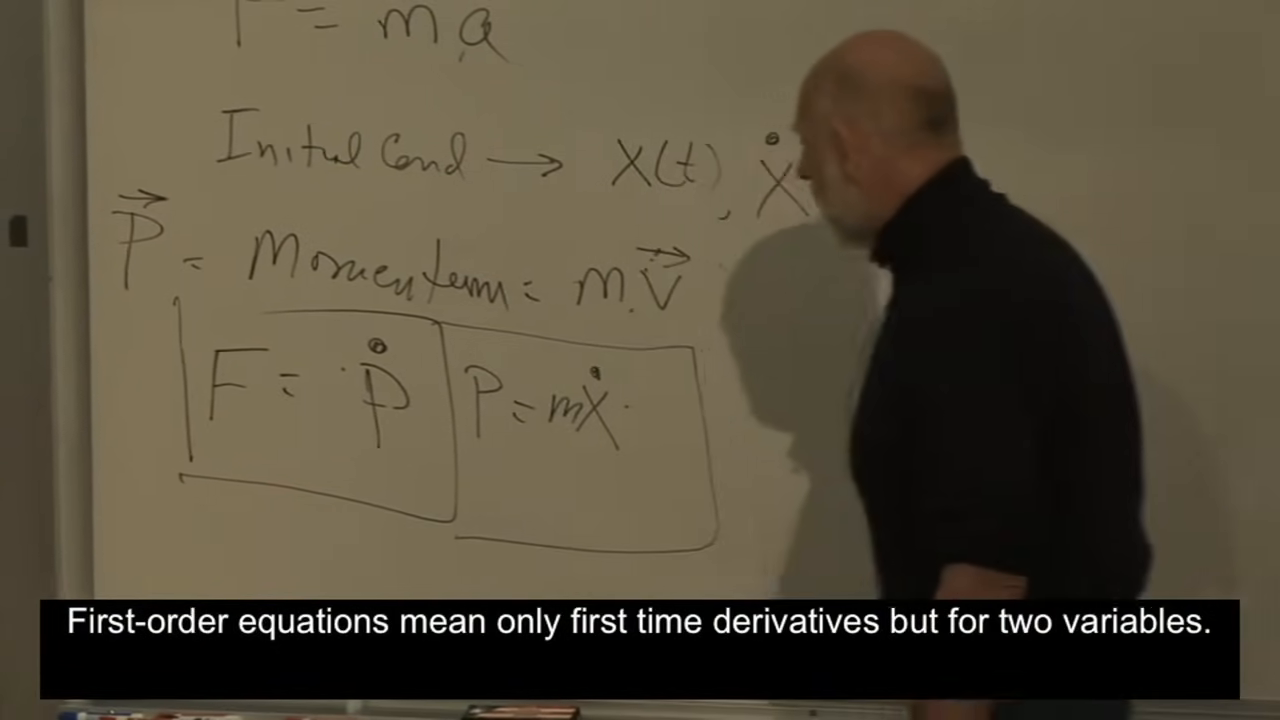
\includegraphics[width=0.84\textwidth]{lecture_02_figure_04.png}\caption{Die beiden Differentialgleichungen erster Ordnung und die zugehörigen Anfangsdaten. Position und Impuls legen gemeinsam den Zustand fest.}\lectureframe{00:35:47}\end{figure}

Der Raum aller Paare \((x,p)\) heißt \emph{Phasenraum}. Für ein Teilchen, das sich in drei Dimensionen bewegt, hat er sechs Koordinaten:

\begin{equation}
  (x,y,z,p_x,p_y,p_z).
  \label{eq:one-particle-phase-space}
\end{equation}

Der Phasenraum ist der Raum vollständiger Anfangsbedingungen. Der Konfigurationsraum erfasst nur Positionen; der Phasenraum enthält genau die Daten, die das Bewegungsgesetz benötigt.

\begin{classroomqa}\audiencequestion{Wird die Aktualisierung komplizierter, wenn die Kraft eine Funktion der Position statt eine bekannte Funktion der Zeit ist?\lecturetimestamp{00:36:27--00:37:07}}\lecturerresponse{Die Gleichungen bleiben vorhersagekräftig. Sobald \(x\) und \(p\) bekannt sind, ist auch der Wert \(F(x)\) bekannt. Gleichung~\eqref{eq:first-order-p} schreitet mit \(p\) fort, Gl.~\eqref{eq:first-order-x} mit \(x\), und das aktualisierte Wertepaar kann erneut verwendet werden.}\end{classroomqa}

\section{Die Newtonsche Feder}

Kehren wir zur Feder zurück, um die beiden Gesetze unter denselben physikalischen Bedingungen zu vergleichen. Nach Newton gilt

\begin{equation}
  m\ddot x=-kx.
  \label{eq:newton-spring}
\end{equation}

Setzen wir vorübergehend \(m=k=1\), um die Konstanten zu entfernen. Dann gilt

\begin{equation}
  \ddot x=-x.
  \label{eq:normalized-oscillator}
\end{equation}

Anders als die Exponentialfunktion kehren Sinus und Kosinus nach zweimaligem Ableiten zu ihrem Negativen zurück. Die allgemeine Lösung lässt sich schreiben als

\begin{align}
  x(t)&=C\cos(t-t_0),
  \label{eq:oscillator-x}\\
  p(t)=\dot x(t)&=-C\sin(t-t_0).
  \label{eq:oscillator-p}
\end{align}

Die beiden Konstanten enthalten die zwei Angaben über den Anfangszustand. Die Amplitude \(C\) gibt die maximale Auslenkung an, während \(t_0\) die Phase festlegt, hier so gewählt, dass die Geschwindigkeit bei \(t=t_0\) null ist. An den Endpunkten kommt das Teilchen nur für einen Augenblick zum Stillstand. Dann kehrt es durch den Ursprung zurück, wo seine Geschwindigkeit und sein Impuls am größten sind, und schwingt weiter.

Quadrieren wir die Gl.~\eqref{eq:oscillator-x} und \eqref{eq:oscillator-p}, erhalten wir

\begin{equation}
  x^2+p^2=C^2.
  \label{eq:oscillator-phase-circle}
\end{equation}

Der Punkt im Phasenraum bewegt sich somit auf einem Kreis mit dem Radius \(C\). Verschiedene Anfangsamplituden ergeben verschiedene Kreise; eine Änderung von \(t_0\) wählt einen anderen Ausgangspunkt auf demselben Kreis. In diesen normierten Einheiten wird jeder Kreis mit derselben Periodendauer \(2\pi\) durchlaufen, unabhängig von der Amplitude.

\begin{figure}[htbp]\centering
  \includegraphics[width=0.84\textwidth]{lecture_02_figure_10.png}\caption{Die Oszillatorlösung und ihre Kreisbahn in der \((x,p)\)-Phasenebene.}\lectureframe{00:43:20}\end{figure}

\begin{figure}[htbp]\centering
  \begin{tikzpicture}[scale=1.05,>=Latex]
    \draw[->] (-2.6,0) -- (2.75,0) node[right] {$x$};
    \draw[->] (0,-2.4) -- (0,2.55) node[above] {$p$};
    \draw[blue!65!black,thick] (0,0) circle (1.85);
    \draw[->,blue!65!black,thick]
      (1.60,0.93) arc[start angle=30,end angle=72,radius=1.85];
    \fill[red!65!black] (1.60,0.93) circle (2pt);
    \draw[dashed] (0,0) -- (1.60,0.93)
      node[midway,below right] {$C$};
    \node[align=left] at (-1.55,1.85)
      {$x=C\cos(t-t_0)$\\$p=-C\sin(t-t_0)$};
  \end{tikzpicture}\caption{Eine Phasenraumtrajektorie bewahrt sowohl Position als auch Impuls. Ihr Radius kennzeichnet die Bewegung, während der Winkel gleichförmig mit der Zeit zunimmt.}\label{fig:oscillator-phase-space}\end{figure}

Die Projektion auf die horizontale Achse ergibt die bekannte Hin- und Herbewegung von \(x\); die Projektion auf die vertikale Achse ergibt die Schwingung von \(p\). Anders als bei der aristotelischen Feder fallen verschiedene Kreise niemals zusammen. Kennt man einen Punkt im Phasenraum, so sind sowohl seine Zukunft als auch seine Vergangenheit bestimmt.

Für allgemeines \(m\) und \(k\) lautet die Kreisfrequenz

\begin{equation}
  \omega=\sqrt{\frac{k}{m}},
  \qquad
  x(t)=C\cos\bigl(\omega(t-t_0)\bigr),
  \label{eq:general-oscillator-frequency}
\end{equation}

und die Phasenraumtrajektorie wird in der nicht skalierten \((x,p)\)-Ebene zu einer Ellipse. Das Kreismodell ist die praktische Normierung \(m=k=1\), die in der Vorlesung verwendet wird.

\begin{classroomqa}\audiencequestion{Ginge die Vorhersagbarkeit verloren, wenn in der Oszillatorgleichung die zweite Ableitung durch eine erste Ableitung ersetzt würde?\lecturetimestamp{00:45:23--00:46:04}}\lecturerresponse{Nein. Auch eine Differentialgleichung erster Ordnung kann die Bewegung ausgehend von geeigneten Anfangsdaten vorhersagen. Die weitergehende Frage ist, ob ihr Fluss Unterschiede ausreichend bewahrt, um umkehrbar zu sein; der entsprechende allgemeine Satz wird erst behandelt, wenn die nötigen mathematischen Mittel bereitstehen.}\end{classroomqa}

\section{Zeitumkehr}

Das Oszillatorbild macht die Umkehrbarkeit anschaulich, doch die Gleichungen lassen sich auch direkt prüfen. Führen wir eine umgekehrte Zeitkoordinate ein:

\begin{equation}
  T=-t.
  \label{eq:reverse-time}
\end{equation}

Dann gilt

\begin{equation}
  \frac{d}{dt}=-\frac{d}{dT},
  \qquad
  \frac{d^2}{dt^2}=\frac{d^2}{dT^2}.
  \label{eq:time-derivative-parity}
\end{equation}

Bei einer Zeitumkehr wechselt eine erste Ableitung ihr Vorzeichen, eine zweite Ableitung dagegen nicht. Folglich behält die autonome aristotelische Gleichung

\begin{equation}
  m\dot x=F(x)
  \label{eq:aristotle-time-reversal}
\end{equation}

ihre Form nicht bei, wenn ein Film rückwärts abgespielt wird. Aus einer abklingenden Feder würde eine Feder, die sich spontan aus dem Gleichgewicht entfernt. Dagegen bleibt

\begin{equation}
  m\ddot x=F(x)
  \label{eq:newton-time-reversal}
\end{equation}

unverändert. Bei der Umkehr eines Newtonschen Films kehrt sich die Geschwindigkeit um, die Beschleunigung bleibt jedoch unverändert; deshalb ist der rückwärts laufende Film ebenfalls eine zulässige Lösung.

\begin{figure}[htbp]\centering
  \includegraphics[width=0.84\textwidth]{lecture_02_figure_11.png}\caption{Vergleich an der Tafel unter \(t\mapsto -t\): Erste Ableitungen wechseln ihr Vorzeichen, zweite Ableitungen dagegen nicht.}\lectureframe{00:50:45}\end{figure}

\begin{classroomqa}\audiencequestion{Warum sollte Umkehrbarkeit als allgemeine Voraussetzung der Physik gelten?\lecturetimestamp{00:46:16--00:48:26}}\lecturerresponse{Sie wird geprüft, nicht durch Definition garantiert. Wir untersuchen erfolgreiche Gesetze, erkennen gemeinsame Merkmale in Experimenten und erheben diese Merkmale zu Prinzipien. Die tiefere logische Ordnung verläuft in die entgegengesetzte Richtung: Die Quantenfeldtheorie ist fundamentaler, und die Newtonsche Mechanik ergibt sich durch Näherungen wie langsame Bewegung und große Massen. Ein Lehrgang muss sich von einfacheren Gesetzen ausgehend aufbauen; deshalb führen wir die Umkehrbarkeit jetzt als Prinzip ein, dessen Geltungsbereich später geprüft wird.}\end{classroomqa}

\begin{classroomqa}\audiencequestion{War die Umkehrbarkeit selbst ein Problem, das Newton bewusst erkannte?\lecturetimestamp{00:48:28--00:49:02}}\lecturerresponse{Die historische Antwort ist ungewiss. Newton verstand sicherlich das Trägheitsprinzip: Eine Kraft ist nötig, um einen Bewegungszustand zu ändern, nicht um eine gleichförmige Bewegung aufrechtzuerhalten. Ob er diese Einsicht ausdrücklich im Hinblick auf Umkehrbarkeit formulierte, ist eine davon getrennte historische Frage.}\end{classroomqa}

\section{Zyklen und Erhaltungsgrößen}

Die Kreise im Phasenraum legen den nächsten Gedanken nahe. Eine Trajektorie bleibt auf einem Kreis und springt niemals auf einen anderen. Der Kreis lässt sich daher durch eine Zahl kennzeichnen, die während der Bewegung konstant bleibt. Für den normierten Oszillator ist diese Zahl

\begin{equation}
  C^2=x^2+p^2.
  \label{eq:cycle-label}
\end{equation}

Bis auf einen Faktor von ein halb ist dies die Energie des Oszillators. Größere Kreise haben eine größere Energie; eine Änderung der Anfangsphase ändert sie nicht. Wir werden diese Aussage herleiten, statt sie lediglich aus dem Bild abzulesen, betrachten aber zunächst den Impuls.

Newtons erstes Gesetz besagt, dass sich ein Gegenstand, auf den keine resultierende Kraft wirkt, mit konstanter Geschwindigkeit bewegt. Es ist bereits im zweiten Gesetz enthalten:

\begin{equation}
  \mathbf F=0
  \quad\Longrightarrow\quad
  \dot{\mathbf p}=0
  \quad\Longrightarrow\quad
  \mathbf v=\text{constant}
  \label{eq:newton-first-from-second}
\end{equation}

bei konstanter Masse. Newtons drittes Gesetz liefert tatsächlich neue Informationen über Wechselwirkungen zwischen Teilchen.

\subsection{Gleich große, entgegengesetzte und zentrale Kräfte}

Die Kraft auf Teilchen \(i\), die von Teilchen \(j\) ausgeübt wird, sei \(\mathbf F_{ij}\). Der Teil des dritten Gesetzes, der gleich große und entgegengesetzte Kräfte betrifft, lautet

\begin{equation}
  \mathbf F_{ij}=-\mathbf F_{ji}.
  \label{eq:newton-third-pair}
\end{equation}

Wiesen die beiden Kräfte in dieselbe Richtung, könnte ein isoliertes Paar spontan beschleunigen. Es wäre eine Maschine ohne Antriebsmittel, die allein durch innere Kräfte Bewegung erzeugt. Ein solches Verhalten wird nicht beobachtet.

\begin{figure}[htbp]\centering
  \includegraphics[width=0.84\textwidth]{lecture_02_figure_12.png}\caption{Die indexierte Aussage über gleich große und entgegengesetzte Wechselwirkungskräfte.}\lectureframe{00:59:25}\end{figure}

Bei den hier betrachteten Punktteilchenkräften wirkt das Kräftepaar außerdem entlang der Verbindungslinie der Teilchenmittelpunkte. Gleich große und entgegengesetzte Kräfte, die nicht auf einer gemeinsamen Wirkungslinie lägen, könnten ein reines Drehmoment bilden und ein isoliertes starres Paar in Drehung versetzen. Die Bedingung der Zentralkraft verhindert diese Möglichkeit:

\begin{equation}
  \mathbf F_{ij}\parallel
  (\mathbf r_i-\mathbf r_j).
  \label{eq:central-force-condition}
\end{equation}

Die Bedingung gleich großer und entgegengesetzter Kräfte führt zur Erhaltung des linearen Impulses. Die Bedingung, dass die Kräfte auf der Verbindungslinie liegen, hängt mit der Erhaltung des Drehimpulses zusammen, die später behandelt wird.

\begin{figure}[htbp]\centering
  \includegraphics[width=0.84\textwidth]{lecture_02_figure_13.png}\caption{Der Zentralcharakter im dritten Newtonschen Gesetz: Wechselwirkungskräfte liegen entlang der Verbindungslinie der Teilchen.}\lectureframe{01:01:38}\end{figure}

\subsection{Gesamtimpuls}

Betrachten wir ein abgeschlossenes System aus \(N\) Teilchen. Es wirken keine äußeren Kräfte; die einzigen Kräfte sind diejenigen, die die Teilchen aufeinander ausüben. Aus der Additivität der Kräfte und Newtons zweitem Gesetz folgt für jedes Teilchen:

\begin{equation}
  \dot{\mathbf p}_i
  =m_i\ddot{\mathbf r}_i
  =\sum_{\substack{j=1\\j\ne i}}^N \mathbf F_{ij}.
  \label{eq:many-particle-newton}
\end{equation}

Summieren wir diese Gleichung über \(i\):

\begin{align}
  \frac{d}{dt}\sum_{i=1}^N\mathbf p_i
  &=\sum_{i=1}^N
    \sum_{\substack{j=1\\j\ne i}}^N\mathbf F_{ij}
  \notag\\
  &=\sum_{i<j}\bigl(\mathbf F_{ij}+\mathbf F_{ji}\bigr)
  =0.
  \label{eq:momentum-pair-cancellation}
\end{align}

Jede Wechselwirkung tritt zweimal auf, einmal in jeder Richtung, und die beiden Beiträge heben sich auf. Definieren wir

\begin{equation}
  \mathbf P_{\mathrm{tot}}=\sum_{i=1}^N\mathbf p_i,
  \label{eq:total-momentum}
\end{equation}

so erhalten wir den ersten Erhaltungssatz:

\begin{equation}
  \frac{d\mathbf P_{\mathrm{tot}}}{dt}=0.
  \label{eq:momentum-conservation}
\end{equation}

\begin{figure}[htbp]\centering
  \includegraphics[width=0.84\textwidth]{lecture_02_figure_14.png}\caption{Bei der Summation der Teilchengleichungen heben sich die paarweisen Kräfte auf; übrig bleibt, dass die Ableitung des Gesamtimpulses null ist.}\lectureframe{01:04:38}\end{figure}

Historisch haben wir die Impulserhaltung als Folge von Newtons drittem Gesetz dargestellt. In der modernen Physik gilt die Impulserhaltung häufig als fundamentalere Aussage: Wenn der Gesamtimpuls eines isolierten Systems aus zwei Teilchen erhalten bleibt, müssen sich ihre inneren Impulsänderungen betragsgleich und entgegengesetzt sein. Für die hier entwickelte Darstellung ist der Newtonsche Weg jedoch zweckmäßig.

\section{Energie in einer Dimension}

Betrachten wir ein Teilchen, das sich entlang einer Geraden unter dem Einfluss einer Kraft bewegt, die nur von seiner Position abhängt:

\begin{equation}
  F=F(x).
  \label{eq:position-force}
\end{equation}

Eine solche Kraft heißt zeitunabhängig. Das bedeutet nicht, dass die auf das bewegte Teilchen wirkende Kraft stets denselben Zahlenwert hat. Ihr Wert ändert sich, wenn sich \(x(t)\) ändert. Gemeint ist, dass das Teilchen an derselben Position \(x\) immer dieselbe Kraft erfährt, unabhängig von der Uhrzeit.

In einer Dimension lässt sich jede hinreichend reguläre Kraftfunktion integrieren. Wir definieren daher eine potenzielle Energie \(V(x)\) durch

\begin{equation}
  F(x)=-\frac{dV}{dx},
  \label{eq:potential-definition-1d}
\end{equation}

oder gleichwertig durch

\begin{equation}
  V(x)=-\int^x F(u)\,du+V_0.
  \label{eq:potential-integral}
\end{equation}

Die additive Konstante \(V_0\) hat keinen Einfluss auf die Kraft. Man kann sich \(V(x)\) als Höhe einer Landschaft über der \(x\)-Achse vorstellen. Das Teilchen wird zu niedrigeren Höhen hin beschleunigt; je steiler das Gefälle, desto größer ist die Kraft. Am Gipfel oder im Tal eines glatten Hügels verschwindet die Steigung und damit auch die Kraft.

\begin{figure}[htbp]\centering
  \includegraphics[width=0.84\textwidth]{lecture_02_figure_15.png}\caption{Die potenzielle Energie als eindimensionale Landschaft. Die Kraft weist bergab; ihr Betrag wird durch die Steigung bestimmt.}\lectureframe{01:12:57}\end{figure}

Definieren wir die kinetische, potenzielle und Gesamtenergie durch

\begin{equation}
  T=\frac12m\dot x^2,
  \qquad
  E=T+V(x)
  =\frac12m\dot x^2+V(x).
  \label{eq:energy-1d}
\end{equation}

An dieser Stelle ist Energie lediglich der Name für diese Größe, die möglicherweise erhalten bleibt. Ihre physikalische Deutung legt die Landschaft nahe: Beim Hinabrollen nimmt \(V\) ab, während die Geschwindigkeit und damit \(T\) zunehmen; beim Hinaufrollen ist es umgekehrt. Newtons Gleichung beweist, dass dieser Austausch exakt ist.

Leiten wir Gl.~\eqref{eq:energy-1d} ab. Da \(m\) konstant ist und \(V\) nur über \(x(t)\) von der Zeit abhängt, gilt

\begin{align}
  \frac{dE}{dt}
  &=m\dot x\ddot x+\frac{dV}{dx}\dot x
  \notag\\
  &=\dot x\left(m\ddot x+\frac{dV}{dx}\right).
  \label{eq:energy-derivative-1d}
\end{align}

Newtons Gesetz und die Definition von \(V\) besagen

\begin{equation}
  m\ddot x=F=-\frac{dV}{dx}.
  \label{eq:newton-potential-1d}
\end{equation}

Der Ausdruck in eckigen Klammern in Gl.~\eqref{eq:energy-derivative-1d} verschwindet daher:

\begin{equation}
  \frac{dE}{dt}=0.
  \label{eq:energy-conservation-1d}
\end{equation}

\begin{figure}[htbp]\centering
  \includegraphics[width=0.84\textwidth]{lecture_02_figure_16.png}\caption{Die Ableitung der eindimensionalen Energie, ausgeklammert als Produkt aus Geschwindigkeit und Newtons Gleichung.}\lectureframe{01:19:18}\end{figure}

In einer Dimension war außer einer regulären, ortsabhängigen Kraft keine zusätzliche dynamische Annahme nötig, denn jede solche Kraft besitzt eine Stammfunktion.

\section{Mehrere Dimensionen und konservative Kräfte}

Für ein Teilchen mit den Koordinaten \(x_i\) lauten die Komponenten von Newtons Gleichung

\begin{equation}
  F_i(\mathbf x)=m\ddot x_i.
  \label{eq:newton-components}
\end{equation}

Die Kraftkomponente \(F_i\) kann von allen Koordinaten abhängen, nicht nur von \(x_i\). Wir möchten eine einzige skalare Funktion \(V(\mathbf x)\) finden, sodass

\begin{equation}
  F_i(\mathbf x)
  =-\frac{\partial V(\mathbf x)}{\partial x_i},
  \qquad
  \mathbf F=-\boldsymbol\nabla V.
  \label{eq:gradient-force}
\end{equation}

Anders als die Konstruktion in einer Dimension ergibt sich das nicht automatisch. Drei beliebige Funktionen \(F_1,F_2,F_3\) enthalten im Allgemeinen mehr unabhängige Information als die Ableitungen einer einzigen skalaren Funktion. Anders ausgedrückt: Ein Potenzial existiert nur dann, wenn das Kraftfeld Kompatibilitätsbedingungen erfüllt, etwa die Gleichheit der entsprechenden gemischten partiellen Ableitungen; in einem einfach zusammenhängenden Gebiet lässt sich dies durch \(\boldsymbol\nabla\times\mathbf F=0\) ausdrücken. Daher nehmen wir Gl.~\eqref{eq:gradient-force} als physikalisches Postulat für die betrachtete Klasse von Kräften an und nicht als mathematische Identität.

\begin{figure}[htbp]\centering
  \includegraphics[width=0.84\textwidth]{lecture_02_figure_17.png}\caption{Das mehrdimensionale Kraftgesetz und eine Skizze der Äquipotenziallinien. Die Kraft weist quer zu den Niveaukurven in Richtung abnehmenden \(V\).}\lectureframe{01:24:15}\end{figure}

Auf einer Niveaulinienkarte ist \(V\) entlang jeder Niveaukurve konstant. Der Gradient steht senkrecht auf diesen Kurven und weist in Richtung des steilsten Anstiegs; die Kraft \(-\boldsymbol\nabla V\) weist in Richtung des steilsten Abstiegs.

\begin{figure}[htbp]\centering
  \begin{tikzpicture}[scale=1.0,>=Latex]
    \draw[->] (-3.0,0) -- (3.1,0) node[right] {$x_1$};
    \draw[->] (0,-2.4) -- (0,2.55) node[above] {$x_2$};
    \draw[orange!65!black,thick]
      plot[smooth cycle] coordinates
      {(-0.55,-0.35) (0.15,-0.55) (0.72,-0.10) (0.50,0.53) (-0.25,0.65)};
    \draw[orange!65!black,thick]
      plot[smooth cycle] coordinates
      {(-1.15,-0.75) (0.20,-1.10) (1.35,-0.25) (1.10,0.95) (-0.45,1.25)};
    \draw[orange!65!black,thick]
      plot[smooth cycle] coordinates
      {(-1.85,-1.20) (0.15,-1.70) (2.15,-0.40) (1.70,1.50) (-0.80,1.85)};
    \draw[->,blue!65!black,very thick] (1.62,0.73) -- (0.82,0.20)
      node[midway,above left] {$\mathbf F$};
    \draw[dashed,->,red!65!black,thick] (0.82,0.20) -- (1.62,0.73)
      node[midway,below right] {$\boldsymbol\nabla V$};
    \node[orange!65!black] at (-1.62,1.45) {$V=V_3$};
    \node[orange!65!black] at (-0.92,0.92) {$V=V_2$};
    \node[orange!65!black] at (-0.35,0.30) {$V=V_1$};
  \end{tikzpicture}\caption{Niveaukurven eines skalaren Potenzials. Der Gradient steht normal auf den Kurven; eine konservative Kraft weist in die entgegengesetzte Richtung.}\label{fig:potential-contours}\end{figure}

Gilt Gl.~\eqref{eq:gradient-force}, definieren wir

\begin{equation}
  E=\frac12m\sum_i\dot x_i^2+V(x_1,\ldots,x_n).
  \label{eq:energy-many-coordinates}
\end{equation}

Der kinetische Term ist die Hälfte der Masse multipliziert mit dem Quadrat des Betrags des Geschwindigkeitsvektors. Durch Ableiten und Anwenden der mehrdimensionalen Kettenregel erhalten wir

\begin{align}
  \frac{dE}{dt}
  &=m\sum_i\dot x_i\ddot x_i
    +\sum_i\frac{\partial V}{\partial x_i}\dot x_i
  \notag\\
  &=\sum_i\dot x_i
    \left(m\ddot x_i+\frac{\partial V}{\partial x_i}\right)
  =0.
  \label{eq:energy-derivative-multidimensional}
\end{align}

Der Beweis entspricht genau dem eindimensionalen Beweis, ergänzt um einen Index; seine Voraussetzung ist jedoch stärker: Alle Kraftkomponenten müssen aus einem gemeinsamen Potenzial hervorgehen.

\begin{figure}[htbp]\centering
  \includegraphics[width=0.84\textwidth]{lecture_02_figure_18.png}\caption{Die indexierte Ableitung der Energie. Jeder Klammerausdruck verschwindet aufgrund der entsprechenden Komponente von Newtons Gleichung.}\lectureframe{01:28:30}\end{figure}

Fassen wir für \(N\) Teilchen in drei Dimensionen alle Koordinaten in einer Liste zusammen:

\begin{equation}
  \begin{aligned}
    q_a={}&(x_1,y_1,z_1,x_2,y_2,z_2,\ldots,\\[-0.2em]
           &\phantom{(}x_N,y_N,z_N),\\
    &a=1,\ldots,3N.
  \end{aligned}
  \label{eq:flattened-coordinates}
\end{equation}

Es gibt \(3N\) Koordinateneinträge, aber nur \(N\) Teilchenmassen; dieselbe Masse gehört zu den drei Einträgen eines jeweiligen Teilchens. Gilt

\begin{equation}
  F_a=-\frac{\partial V(q_1,\ldots,q_{3N})}{\partial q_a},
  \label{eq:many-particle-conservative-force}
\end{equation}

dann

\begin{equation}
  E=\sum_{A=1}^{N}\frac12m_A\lvert\dot{\mathbf r}_A\rvert^2
    +V(\mathbf r_1,\ldots,\mathbf r_N)
  \label{eq:many-particle-energy}
\end{equation}

ist auch diese Größe aufgrund derselben Rechnung erhalten. Kräfte, die aus einem Potenzial hervorgehen, heißen gerade deshalb \emph{konservativ}, weil sie diesen Erhaltungssatz ermöglichen; das Adjektiv hat keine politische Bedeutung.

\section{Der Oszillator als Energiekontur}\enlargethispage{3\baselineskip}

Für die Federkraft \(F=-kx\) ergibt sich aus Gl.~\eqref{eq:potential-definition-1d}

\begin{equation}
  V(x)=\frac12kx^2+V_0.
  \label{eq:spring-potential}
\end{equation}

Wählen wir \(V_0=0\), so ist die Energie des Oszillators

\begin{equation}
  E=\frac12m\dot x^2+\frac12kx^2
   =\frac{p^2}{2m}+\frac12kx^2.
  \label{eq:oscillator-energy}
\end{equation}

Für \(m=k=1\) gilt

\begin{equation}
  2E=p^2+x^2=C^2.
  \label{eq:oscillator-energy-circle}
\end{equation}

Die zuvor gefundenen Kreise im Phasenraum sind demnach Linien konstanter Energie. Bei einem allgemeineren eindimensionalen Potenzial müssen die Konturen keine Kreise sein, doch die Bewegung verläuft weiterhin auf Kurven

\begin{equation}
  \frac{p^2}{2m}+V(x)=E
  \label{eq:general-energy-contour}
\end{equation}

in der \((x,p)\)-Ebene. Damit gelangen wir zurück zu einem Gedanken aus der ersten Vorlesung: Wenn Trajektorien auf verschiedenen Zyklen oder Bahnen bleiben, kann eine Zahl diese Bahnen kennzeichnen und während der gesamten Bewegung unverändert bleiben.

Damit haben wir nun den Zustandsraum, die Newtonschen Aktualisierungsgleichungen und die ersten beiden Erhaltungssätze. Die nächste Formulierung der Mechanik geht vom Prinzip der kleinsten Wirkung aus und führt zu Lagrangefunktionen, Hamiltonfunktionen, Drehimpuls und der allgemeineren Struktur, die hinter diesen Beispielen steht.

\begin{classroomqa}\audiencequestion{Wie genau stimmen das verteilte Skript und die Arbeit an der Tafel überein, und wo sind die Abbildungen?\lecturetimestamp{01:37:56--01:38:54}}\lecturerresponse{Das Skript sollte der Vorlesung genau folgen; fehlt darin Stoff von der Tafel, könnte die falsche Datei verschickt worden sein. Die Abbildungen waren noch nicht fertig; sie würden, scherzt er, erscheinen, sobald Continuing Studies den nächsten Scheck bezahlt hätte.}\end{classroomqa}
\chapter{Stationäre Wirkung und die Euler--Lagrange-Gleichung}

\lectureoverview{Der geläufige Name \emph{Prinzip der kleinsten Wirkung} verdeckt den wesentlichen Punkt: Die physikalische Bahn macht die Wirkung stationär, muss sie aber nicht minimieren. Wir werden diese Aussage ausgehend vom gewöhnlichen Gleichgewicht entwickeln, sie von Punkten auf ganze Funktionen übertragen, die Euler--Lagrange-Gleichung durch Diskretisierung einer Bahn herleiten und die Newtonschen Gleichungen wiedergewinnen. Anschließend zeigen Dreh- und Polarkoordinaten, warum die Lagrange-Formulierung mehr als eine bloße Änderung der Schreibweise ist.}

\section{Stationär, aber nicht notwendigerweise minimal}

Der unzuverlässige Teil des traditionellen Namens ist das Wort \emph{kleinsten}. Eine klassische Bahn macht die Wirkung nicht immer minimal. Im Raum der möglichen Bahnen kann sie stattdessen auch ein Maximum oder einen Sattelpunkt ergeben. Das korrekte Prinzip lautet, dass die Wirkung \emph{stationär} ist: Ihre Änderung erster Ordnung verschwindet.

Beginnen wir mit der einfacheren Frage nach dem Gleichgewicht. Ein Teilchen, das in Ruhe bleibt, hat keine Beschleunigung; folglich muss die resultierende Kraft verschwinden. Für eine Kraft, die sich aus einem eindimensionalen Potenzial ableitet, gilt
\begin{equation}
  F(x)=-\frac{dV}{dx},
  \label{eq:force-from-v}
\end{equation}
Die Gleichgewichtsbedingung lautet
\begin{equation}
  \frac{dV}{dx}=0.
  \label{eq:stationary-v-one}
\end{equation}

\begin{figure}[htbp]
  \centering
  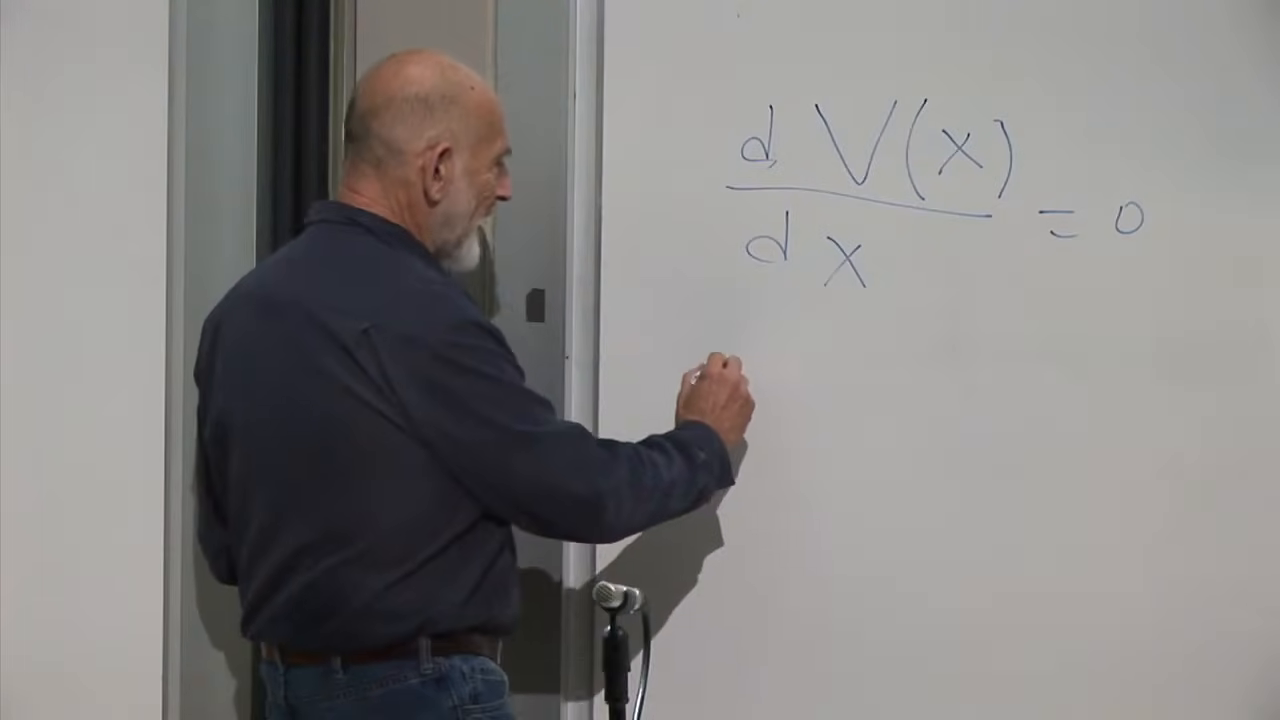
\includegraphics[width=0.74\textwidth]{lecture_03_figure_02.png}
  \caption{Die eindimensionale Gleichgewichtsbedingung: Die Kraft verschwindet dort, wo das Potenzial stationär ist.}
  \lectureframe{00:02:51}
\end{figure}

Verschieben wir das Teilchen nun um einen kleinen Betrag \(\delta x\). In erster Ordnung gilt
\begin{equation}
  \delta V
  =V(x+\delta x)-V(x)
  =\frac{dV}{dx}\,\delta x+O(\delta x^2).
  \label{eq:first-variation-one}
\end{equation}
Im Gleichgewicht verschwindet der lineare Term für beide Vorzeichen von \(\delta x\):
\begin{equation}
  \delta V=0
  \qquad\hbox{to first order.}
  \label{eq:delta-v-zero-one}
\end{equation}
Das bedeutet nicht, dass \(V\) sich nach einer endlichen Verschiebung exakt nicht ändert. Es besagt, dass die führende Änderung quadratisch oder von höherer Ordnung ist. Sowohl ein Minimum als auch ein Maximum erfüllen diese Bedingung.

\begin{figure}[htbp]
  \centering
  \begin{tikzpicture}[scale=0.95,>=Latex]
    \draw[->] (-0.2,0) -- (3.35,0) node[right] {$x$};
    \draw[->] (0,-0.2) -- (0,2.25) node[above] {$V$};
    \draw[blue!65!black,thick,smooth]
      plot coordinates {(0.2,1.85) (0.75,0.85) (1.55,0.35)
                        (2.35,0.85) (3.0,1.85)};
    \fill[red!65!black] (1.55,0.35) circle (2pt);
    \node at (1.55,-0.34) {minimum};
    \begin{scope}[xshift=4.25cm]
      \draw[->] (-0.2,0) -- (3.35,0) node[right] {$x$};
      \draw[->] (0,-0.2) -- (0,2.25) node[above] {$V$};
      \draw[blue!65!black,thick,smooth]
        plot coordinates {(0.2,0.35) (0.75,1.25) (1.55,1.85)
                          (2.35,1.25) (3.0,0.35)};
      \fill[red!65!black] (1.55,1.85) circle (2pt);
      \node at (1.55,-0.34) {maximum};
    \end{scope}
  \end{tikzpicture}
  \caption{Die Stationarität legt die erste Ableitung fest, nicht aber, ob der Punkt ein Minimum oder ein Maximum ist.}
  \label{fig:min-max-stationary}
\end{figure}

Für viele Koordinaten \(q_i\) lautet die erste Variation
\begin{equation}
  \delta V
  =\sum_i\frac{\partial V}{\partial q_i}\,\delta q_i.
  \label{eq:first-variation-many}
\end{equation}
Soll sie für jede unabhängige infinitesimale Verschiebung \(\delta q_i\) verschwinden, muss jeder Koeffizient verschwinden:
\begin{equation}
  \frac{\partial V}{\partial q_i}=0
  \qquad\hbox{for every }i.
  \label{eq:stationary-v-many}
\end{equation}

Ein zweidimensionales Potenzial stellt man sich besser als hügeliges Gelände denn als Achterbahn vor. Ein stationärer Punkt kann am Grund eines Tals, auf einem Gipfel oder an einem Sattel liegen. Am Sattel führt eine anfängliche Bewegung in eine Richtung bergauf, in einer anderen dagegen bergab. Das rücktreibende Verhalten kann daher in einer Richtung stabil und in einer anderen instabil sein, obwohl am Punkt selbst alle ersten Ableitungen verschwinden.

\begin{figure}[htbp]
  \centering
  \includegraphics[width=0.76\textwidth]{lecture_03_figure_06.png}
  \caption{Ein Sattelpunkt ist in jeder Richtung stationär in erster Ordnung, obwohl benachbarte Verschiebungen entlang der einen Achse ansteigen und entlang einer anderen abfallen.}
  \lectureframe{00:08:20}
\end{figure}

In einem Raum mit vielen Koordinaten sind Sattelpunkte typischer als reine Maxima oder Minima. Deshalb ist \emph{stationär} der treffendere Begriff. Die Bedingung
\begin{equation}
  \delta V=0
  \label{eq:equilibrium-variation}
\end{equation}
beschreibt das Gleichgewicht, ohne das Verhalten zweiter Ordnung vorwegzunehmen.

\section{Von Punkten zu Funktionen}

Die Mechanik befasst sich mit ganzen Bewegungen, nicht mit isolierten Gleichgewichtspunkten. Eine Bahn ist eine Funktion wie \(x(t)\) oder eine Sammlung von Funktionen wie \((x(t),y(t),z(t))\). Das mathematische Problem, eine Größe durch Variation einer ganzen Funktion stationär zu machen, heißt \emph{Variationsrechnung}. Bevor wir sie auf Bewegungen anwenden, betrachten wir drei einfachere Beispiele.

\subsection{Kürzeste Kurven und Geodäten}

Wir betrachten zwei feste Punkte in der Ebene und stellen eine Kurve zwischen ihnen durch \(y(x)\) dar. Für ein kurzes Kurvenstück gilt
\begin{equation}
  ds=\sqrt{dx^2+dy^2}
  =dx\sqrt{1+\left(\frac{dy}{dx}\right)^2},
  \label{eq:line-element}
\end{equation}
wobei die letzte Form \(dx>0\) voraussetzt. Die Gesamtlänge ist das Funktional
\begin{equation}
  S[y]=\int_{x_0}^{x_1}
  \sqrt{1+y'(x)^2}\,dx.
  \label{eq:arc-length-functional}
\end{equation}
Die eckigen Klammern betonen, dass \(S\) eine ganze Funktion als Eingabe erhält. Die Gerade ergibt sich aus der Bedingung
\begin{equation}
  \delta S=0
  \label{eq:stationary-length}
\end{equation}
bei kleinen Änderungen der Kurve, die beide Endpunkte festhalten.

\begin{figure}[htbp]
  \centering
  \includegraphics[width=0.78\textwidth]{lecture_03_figure_07.png}
  \caption{Eine Probekurve zwischen zwei festen Endpunkten. Ihre Länge ist die Summe der infinitesimalen Hypotenusen \(ds\).}
  \lectureframe{00:13:36}
\end{figure}

Dieselbe Frage lässt sich auf einer gekrümmten Fläche stellen. Zieht man eine Schnur zwischen zwei Pflöcken straff, erhält man ein anschauliches Bild des kürzesten Weges unter den gegebenen Einschränkungen. Eine solche Kurve mit stationärer Länge heißt \emph{Geodäte}. In einer flachen Ebene ist sie eine Gerade; auf einer Kugel oder einer hügeligen Fläche im Allgemeinen nicht.

\subsection{Fermatsches Prinzip}

Ein Lichtstrahl in einem Medium, dessen Ausbreitungsgeschwindigkeit ortsabhängig ist, \(c(x,y)\) muss nicht den räumlich kürzesten Weg nehmen. Die für ein kurzes Wegstück benötigte Zeit ist die Strecke geteilt durch die lokale Geschwindigkeit, also
\begin{equation}
  T[y]
  =\int_{x_0}^{x_1}
  \frac{\sqrt{1+y'(x)^2}}{c(x,y)}\,dx.
  \label{eq:fermat-functional}
\end{equation}
Nach dem Fermatschen Prinzip gilt
\begin{equation}
  \delta T=0.
  \label{eq:fermat-stationary}
\end{equation}
Ist \(c\) konstant, reduziert sich dies auf das Problem der kürzesten Strecke. In einem Medium mit variablem Brechungsindex gleicht der schnellste Weg dagegen die Streckenlänge und die lokale Ausbreitungsgeschwindigkeit gegeneinander ab.

\begin{figure}[htbp]
  \centering
  \includegraphics[width=0.80\textwidth]{lecture_03_figure_08.png}
  \caption{Das Funktional der Laufzeit eines Lichtstrahls in einem Medium, dessen lokale Lichtgeschwindigkeit vom Ort abhängt.}
  \lectureframe{00:22:50}
\end{figure}

Ein zeitgebundener Scherz spielt auf die damals neue Behauptung an, Neutrinos hätten sich in Italien ungewöhnlich schnell bewegt. Das physikalische Argument kehrt sofort zum verlässlichen Beispiel zurück: Gewöhnliches Licht ändert in Materie seine Geschwindigkeit entsprechend dem Brechungsindex.

\subsection{Eine hängende Kette}

Eine an zwei Punkten befestigte Kette nimmt die Form einer Kettenlinie an. Jedes kleine Stück trägt zur gravitativen potenziellen Energie bei, sodass die gesamte potenzielle Energie selbst ein Integral über die Kette ist. Wieder sind die Endpunkte fest, die unbekannte Form ist eine Funktion und ein Integral muss stationär sein.

\begin{figure}[htbp]
  \centering
  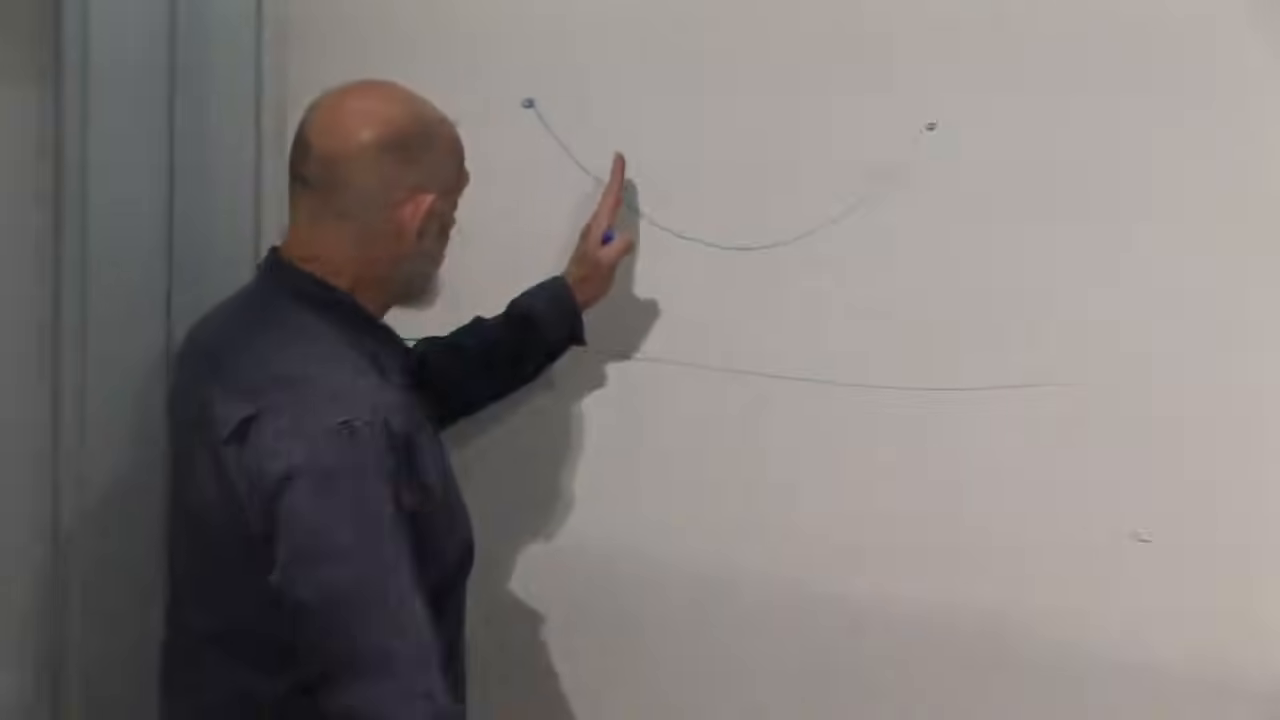
\includegraphics[width=0.76\textwidth]{lecture_03_figure_03.png}
  \caption{Eine hängende Kette zwischen festen Aufhängungen. Ihre stationäre Form wird durch die gesamte gravitative potenzielle Energie bestimmt.}
  \lectureframe{00:30:41}
\end{figure}

Diese Beispiele haben denselben Aufbau: zwei feste Endpunkte, eine Funktion zwischen ihnen und ein Integral, dessen erste Variation verschwindet. Ein solches globales Prinzip auf eine Differentialgleichung zurückzuführen, bedeutet, das Variationsproblem zu lösen.

\section{Mechanik als Randwertproblem}

Eine Bahn wird häufig mit horizontaler Zeitachse gezeichnet, weil \(t\) die unabhängige Variable ist. In der Physik gibt es dennoch die feste Konvention, die Zeit nach oben aufzutragen. Eine Randbemerkung erinnert an Experimente, bei denen Menschen Bilder von der Jugend bis ins Alter in der für ihr Schriftsystem üblichen Richtung anordneten: Leserinnen und Leser von links nach rechts ordneten sie meist von links nach rechts, Leserinnen und Leser von rechts nach links in die Gegenrichtung und vertikal Schreibende vertikal. Der Scherz schließt mit der Bemerkung, Physiker seien diejenigen, die darauf bestehen, dass die Zeit nach oben fließt. Hier verwenden wir die übliche horizontale \(t\)-Achse, weil sich \(x(t)\) so natürlich als Graph darstellen lässt.

Bei der Anfangswertformulierung lauten die Daten zum Zeitpunkt \(t_0\)
\begin{equation}
  x(t_0)=x_0,
  \qquad
  \dot x(t_0)=v_0.
  \label{eq:initial-value-data}
\end{equation}
Die Newtonsche Gleichung bestimmt dann die weitere Bahn. Eine Variationsformulierung stellt ein anderes Problem: Man gibt zwei Endereignisse vor,
\begin{equation}
  x(t_0)=x_0,
  \qquad
  x(t_1)=x_1,
  \label{eq:boundary-value-data}
\end{equation}
und bestimmt den physikalischen Weg dazwischen. Die Anfangsgeschwindigkeit wird nicht mehr vorgegeben, sondern ist Teil der Lösung.

\begin{figure}[htbp]
  \centering
  \includegraphics[width=0.76\textwidth]{lecture_03_figure_09.png}
  \caption{Eine mechanische Bahn \(x(t)\). Man kann entweder Position und Steigung an einem Ende oder die Positionen zu zwei Endzeitpunkten vorgeben.}
  \lectureframe{00:27:41}
\end{figure}

Die stationär zu machende Größe ist die \emph{Wirkung},
\begin{equation}
  A[x]=\int_{t_0}^{t_1}L(x,\dot x,t)\,dt.
  \label{eq:action-one}
\end{equation}
Der Integrand \(L\) ist die \emph{Lagrange-Funktion}. Sie kann von Ort und Geschwindigkeit sowie explizit von der Zeit abhängen. Das Wirkungsprinzip lautet
\begin{equation}
  \delta A=0
  \label{eq:stationary-action}
\end{equation}
für alle kleinen Bahnvariationen mit
\begin{equation}
  \delta x(t_0)=\delta x(t_1)=0.
  \label{eq:fixed-endpoint-variations}
\end{equation}
Die Randbedingung ist wesentlich: Verglichen werden benachbarte Bahnen, die dieselben beiden Ereignisse verbinden.

\section{Eine diskrete Herleitung der Euler--Lagrange-Gleichung}

Die Wirkung ist ein Funktional von unendlich vielen Werten der Bahn. Um ihre Variation konkret zu machen, teilen wir das Zeitintervall in Schritte der Länge \(\epsilon\) ein,
\begin{equation}
  t_n=t_0+n\epsilon,
  \qquad
  x_n=x(t_n),
  \label{eq:discrete-times}
\end{equation}
und nähern die Geschwindigkeit im \(n\)-ten Intervall an durch
\begin{equation}
  v_n=\frac{x_{n+1}-x_n}{\epsilon}.
  \label{eq:discrete-velocity}
\end{equation}
Das Integral wird damit zur gewöhnlichen Summe
\begin{equation}
  A_\epsilon
  =\sum_{n=0}^{N-1}
  \epsilon L\left(x_n,\frac{x_{n+1}-x_n}{\epsilon}\right).
  \label{eq:discrete-action}
\end{equation}
Für die Bezeichnung der Zeitschritte verwenden wir \(n\), damit \(i\) später für räumliche Koordinaten und Teilchen zur Verfügung steht.

\begin{figure}[htbp]
  \centering
  \includegraphics[width=0.82\textwidth]{lecture_03_figure_10.png}
  \caption{Die Bahn wird durch eine Kette von Zeitschritten ersetzt. Die Variation einer inneren Höhe verändert nur die beiden benachbarten Segmente.}
  \lectureframe{00:38:30}
\end{figure}

Wir variieren einen inneren Punkt \(x_n\) und halten alle übrigen \(x_k\) fest. Nur zwei Terme der Summe hängen von \(x_n\) ab:
\begin{align}
  A_\epsilon\big|_{x_n}
  &=
  \epsilon L\left(x_n,\frac{x_{n+1}-x_n}{\epsilon}\right)
  \notag\\
  &\quad+
  \epsilon L\left(x_{n-1},
                  \frac{x_n-x_{n-1}}{\epsilon}\right).
  \label{eq:two-neighbor-terms}
\end{align}
Durch Ableiten erhalten wir
\begin{align}
  0=\frac{\partial A_\epsilon}{\partial x_n}
  &=
  \epsilon\frac{\partial L_n}{\partial x_n}
  -\frac{\partial L_n}{\partial v_n}
  +\frac{\partial L_{n-1}}{\partial v_{n-1}}.
  \label{eq:discrete-el-variation}
\end{align}
Die entgegengesetzten Vorzeichen haben einen einfachen geometrischen Ursprung. Wird \(x_n\) angehoben, nimmt die Steigung des dahinterliegenden Intervalls zu und die des davorliegenden Intervalls ab.

\begin{figure}[htbp]
  \centering
  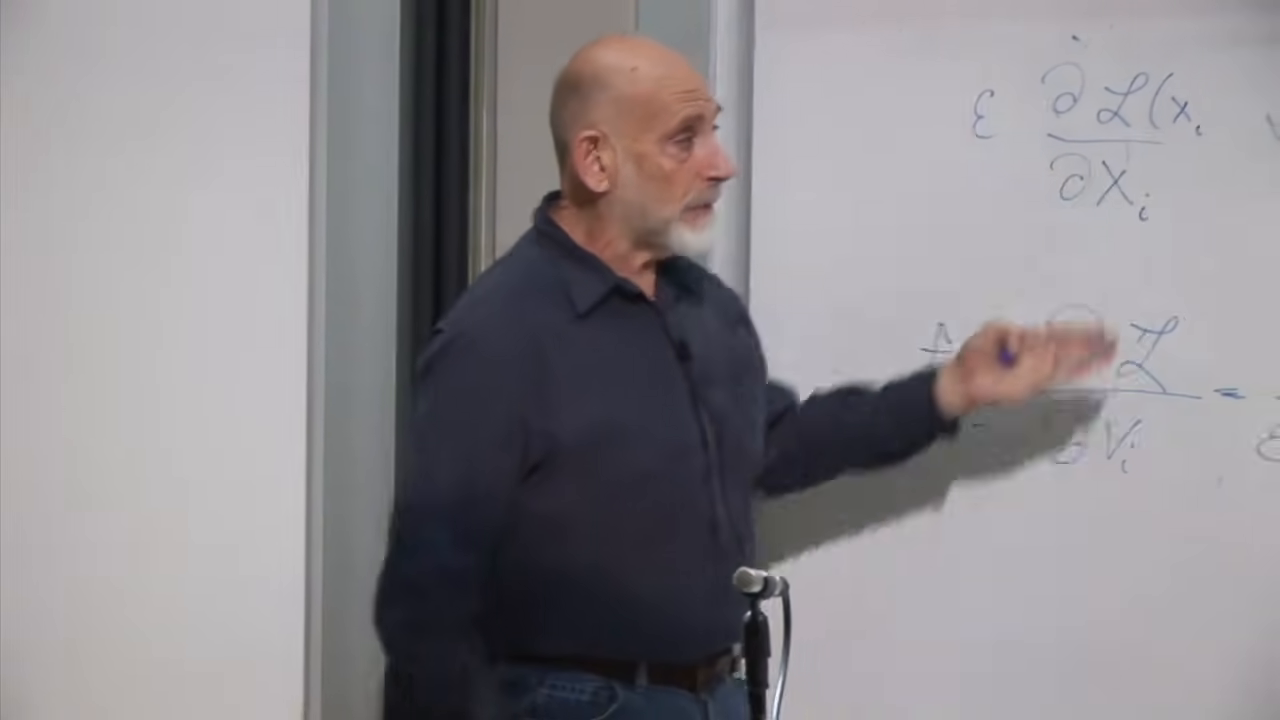
\includegraphics[width=0.74\textwidth]{lecture_03_figure_04.png}
  \caption{Der direkte Ableitungsbeitrag nach dem Ort und die beiden Beiträge der Ableitungen nach der Geschwindigkeit aus den benachbarten Intervallen bei der diskreten Variation.}
  \lectureframe{00:45:26}
\end{figure}

Stellen wir Gl.~\eqref{eq:discrete-el-variation} um:
\begin{equation}
  \frac{1}{\epsilon}
  \left(
    \frac{\partial L_n}{\partial v_n}
    -\frac{\partial L_{n-1}}{\partial v_{n-1}}
  \right)
  =
  \frac{\partial L_n}{\partial x_n}.
  \label{eq:discrete-el}
\end{equation}
Die linke Seite ist ein Differenzenquotient benachbarter Werte. Für \(\epsilon\to0\) wird aus der gebrochenen Linie eine glatte Bahn und der Quotient eine Zeitableitung:
\begin{equation}
  \boxed{
  \frac{d}{dt}\left(\frac{\partial L}{\partial\dot x}\right)
  =
  \frac{\partial L}{\partial x}}
  .
  \label{eq:euler-lagrange-one}
\end{equation}
Dies ist die Euler--Lagrange-Gleichung.

\begin{figure}[htbp]
  \centering
  \includegraphics[width=0.78\textwidth]{lecture_03_figure_11.png}
  \caption{Die vollständige Euler--Lagrange-Gleichung, die sich aus der Stationarität an jedem inneren Zeitschritt ergibt.}
  \lectureframe{00:49:25}
\end{figure}

Sobald \(L\) festgelegt ist, funktioniert Gl.~\eqref{eq:euler-lagrange-one} wie eine Rechenvorschrift: Man leitet die gegebene Funktion ab und erhält eine Differentialgleichung für die Bahn.

\begin{classroomqa}\audiencequestion{Gilt das Ergebnis von Euler--Lagrange für jede Funktion von \(x\) und \(\dot x\)?\lecturetimestamp{00:49:37--00:50:24}}\lecturerresponse{Ja, sofern die für die Ableitungen erforderliche Regularität gegeben ist. Beim Beispiel der Bogenlänge erhält man genau dieselbe Form, wenn man die unabhängige Variable \(x\) der Rolle von \(t\) und die gesuchte Funktion \(y(x)\) der Rolle von \(x(t)\) zuordnet. Die Lösungen der zugehörigen Euler--Lagrange-Gleichung sind Geraden.}\end{classroomqa}

\section{Newtons Gleichungen aus der Lagrange-Funktion}

Für ein Teilchen auf einer Geraden im Potenzial \(V(x)\) wählen wir
\begin{equation}
  L(x,\dot x)=T-V
  =\frac12m\dot x^2-V(x).
  \label{eq:lagrangian-tv-one}
\end{equation}
Das Minuszeichen mag seltsam erscheinen, weil die Gesamtenergie \(T+V\) ist. Doch die Lagrange-Funktion ist nicht die Energie. Entscheidend ist, ob die Euler--Lagrange-Vorschrift die richtige Bewegung ergibt. Eine scherzhafte Abstimmung über das Vorzeichen wird abgelehnt: Die Antwort muss überprüft, nicht gewählt werden.

Zunächst gilt
\begin{equation}
  \frac{\partial L}{\partial\dot x}=m\dot x.
  \label{eq:conjugate-momentum-one}
\end{equation}
Dies ist der Impuls. Allgemeiner ist der einer beliebigen Koordinate \(q\) konjugierte Impuls definiert durch
\begin{equation}
  p_q=\frac{\partial L}{\partial\dot q}.
  \label{eq:conjugate-momentum-general}
\end{equation}
Die Zeitableitung von Gl.~\eqref{eq:conjugate-momentum-one} ergibt \(m\ddot x\), während
\begin{equation}
  \frac{\partial L}{\partial x}
  =-\frac{dV}{dx}.
  \label{eq:lagrangian-position-derivative}
\end{equation}
Damit lautet die Euler--Lagrange-Gleichung
\begin{equation}
  m\ddot x=-\frac{dV}{dx}=F(x),
  \label{eq:newton-from-action}
\end{equation}
also das zweite Newtonsche Gesetz.

\begin{figure}[htbp]
  \centering
  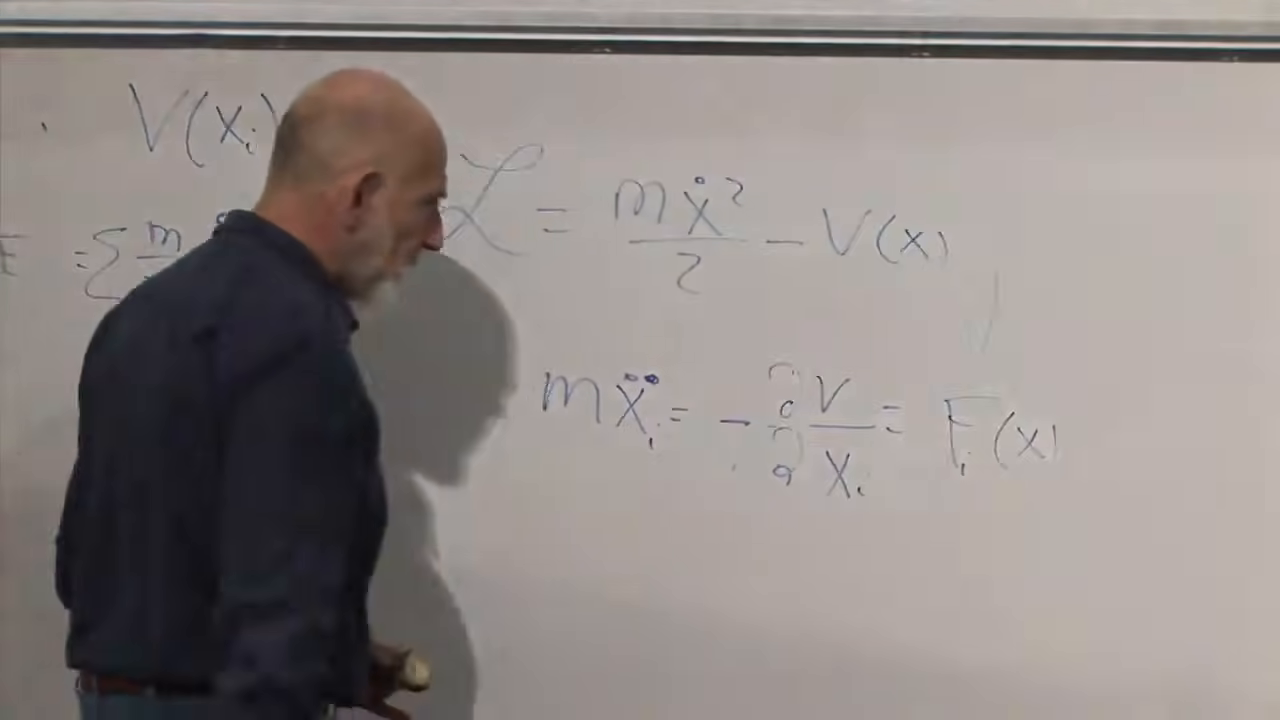
\includegraphics[width=0.80\textwidth]{lecture_03_figure_05.png}
  \caption{Kinetische Energie, potenzielle Energie, \(L=T-V\) und die wiedergewonnene Komponentenform der Newtonschen Gleichung an einer Tafel.}
  \lectureframe{00:57:52}
\end{figure}

Für viele Koordinaten \(q_i\) gilt
\begin{equation}
  L(\mathbf q,\dot{\mathbf q})
  =\sum_i\frac12m_i\dot q_i^{\,2}-V(q_1,q_2,\ldots),
  \label{eq:lagrangian-tv-many}
\end{equation}
und für jede Koordinate gibt es eine Gleichung:
\begin{equation}
  \frac{d}{dt}\left(\frac{\partial L}{\partial\dot q_i}\right)
  =\frac{\partial L}{\partial q_i}
  \quad\Longrightarrow\quad
  m_i\ddot q_i=-\frac{\partial V}{\partial q_i}=F_i.
  \label{eq:euler-lagrange-many}
\end{equation}
Die Bahn bleibt eine einzige Kurve, verläuft nun aber durch einen hochdimensionalen Konfigurationsraum.

\begin{classroomqa}\audiencequestion{Sind wir nicht einfach vom Newtonschen Gesetz rückwärts ausgegangen und haben ein Funktional so konstruiert, dass es das Ergebnis reproduziert?\lecturetimestamp{00:58:07--01:00:04}}\lecturerresponse{Das ist keine zielführende Sichtweise. Die Lagrange-Funktion ist die kompakte Beschreibung des physikalischen Systems: Eine Funktion aller Koordinaten und Geschwindigkeiten fasst sämtliche Bewegungsgleichungen zusammen. Bei neuen Theorien schlagen Physiker gewöhnlich eine Wirkung vor und leiten daraus die Gleichungen her, statt jede Gleichung einzeln zu erraten.}\end{classroomqa}

Diese Zusammenfassung ist ein Vorteil. Die Freiheit der Koordinaten ist ein weiterer. Die Aussage, dass eine Linie die kürzeste ist, hängt nicht davon ab, ob die Ebene mit kartesischen, polaren oder krummlinigen Koordinaten beschrieben wird. Ebenso ist die Stationarität der Wirkung koordinatenunabhängig, auch wenn sich die Formel für \(L\) und die daraus folgenden Komponentengleichungen ändern.

\section{Ein freies Teilchen vom Karussell aus gesehen}

Seien \((x,y)\) inertiale kartesische Koordinaten und \((X,Y)\) kartesische Koordinaten, die sich gleichförmig mit der Winkelgeschwindigkeit \(\omega\) drehen. Bei der hier verwendeten Orientierung gilt
\begin{align}
  x&=X\cos\omega t+Y\sin\omega t,
  \notag\\
  y&=-X\sin\omega t+Y\cos\omega t.
  \label{eq:rotating-coordinate-map}
\end{align}
Der Winkel zwischen den Bezugssystemen beträgt \(\omega t\).

\begin{figure}[htbp]
  \centering
  \includegraphics[width=0.76\textwidth]{lecture_03_figure_12.png}
  \caption{Inertiale und gleichförmig rotierende kartesische Achsen. Derselbe Punkt erhält zeitabhängige rotierende Koordinaten.}
  \lectureframe{01:06:05}
\end{figure}

Die Lagrange-Funktion eines freien Teilchens im Inertialsystem lautet
\begin{equation}
  L_{\mathrm{in}}
  =\frac{m}{2}\left(\dot x^2+\dot y^2\right).
  \label{eq:free-inertial-lagrangian}
\end{equation}
Leiten wir Gl.~\eqref{eq:rotating-coordinate-map} ab und verwenden \(\sin^2\omega t+\cos^2\omega t=1\). Die trigonometrischen Terme lassen sich zusammenfassen zu
\begin{align}
  \dot x^2+\dot y^2
  &=
  \dot X^2+\dot Y^2\\
  &\quad+\omega^2(X^2+Y^2)\\
  &\quad+2\omega(Y\dot X-X\dot Y).
  \label{eq:rotating-speed}
\end{align}
Somit gilt
\begin{align}
  L_{\mathrm{rot}}
  &=
  \frac{m}{2}(\dot X^2+\dot Y^2)\\
  &\quad+\frac{m\omega^2}{2}(X^2+Y^2)\\
  &\quad+m\omega(Y\dot X-X\dot Y).
  \label{eq:rotating-lagrangian}
\end{align}

\begin{figure}[htbp]
  \centering
  \includegraphics[width=0.84\textwidth]{lecture_03_figure_13.png}
  \caption{Die transformierte Lagrange-Funktion des freien Teilchens: gewöhnliche kinetische Energie, ein quadratischer Zentrifugalterm und ein linearer Geschwindigkeitsterm.}
  \lectureframe{01:12:16}
\end{figure}

Der quadratische Koordinatenterm hat die Form \(-V_{\mathrm{fict}}\), wobei
\begin{equation}
  V_{\mathrm{fict}}
  =-\frac{m\omega^2}{2}(X^2+Y^2).
  \label{eq:centrifugal-potential}
\end{equation}
Das entsprechende Potenzial nimmt nach außen hin ab und erzeugt daher die Zentrifugalkraft \(m\omega^2(X,Y)\).

Der letzte Term in Gl.~\eqref{eq:rotating-lagrangian} ist sowohl in den Koordinaten als auch in den Geschwindigkeiten linear. Die Euler--Lagrange-Gleichung liefert
\begin{align}
  m\ddot X&=m\omega^2X-2m\omega\dot Y,
  \notag\\
  m\ddot Y&=m\omega^2Y+2m\omega\dot X.
  \label{eq:rotating-equations}
\end{align}
Die Terme proportional zu \(\omega^2\) sind Zentrifugalterme; die geschwindigkeitsproportionalen Terme sind Coriolis-Terme. In Vektorform innerhalb der rotierenden Ebene gilt
\begin{equation}
  \mathbf F_{\mathrm{C}}
  =-2m\,\boldsymbol\omega\times\mathbf v_{\mathrm{rot}},
  \label{eq:coriolis-vector}
\end{equation}
wobei sich die Vorzeichen ändern, wenn die entgegengesetzte Orientierungskonvention verwendet wird.

\begin{figure}[htbp]
  \centering
  \includegraphics[width=0.84\textwidth]{lecture_03_figure_14.png}
  \caption{Die Gleichungen im rotierenden Bezugssystem: Die koordinatenproportionalen Terme liefern Zentrifugalbeschleunigungen, die geschwindigkeitsabhängigen Kreuzterme Coriolisbeschleunigungen.}
  \lectureframe{01:20:20}
\end{figure}

Der Punkt ist nicht, dass die Algebra wegfällt. Vielmehr erzeugt eine einzige Koordinatentransformation einer einzelnen skalaren Funktion beide gekoppelten Gleichungen und beide Scheinkräfte.

\begin{classroomqa}\audiencequestion{Funktioniert diese Methode auch für beliebig gekrümmte Koordinaten?\lecturetimestamp{01:22:01--01:22:17}}\lecturerresponse{Ja. Die neuen Koordinaten können krummlinig sein und sogar explizit von der Zeit abhängen, wie es bei den rotierenden Koordinaten der Fall ist. Man schreibt die Wirkung in den neuen Variablen um und wendet dieselbe Euler--Lagrange-Regel an.}\end{classroomqa}

\section{Polarkoordinaten und ein zyklischer Winkel}

Für gewöhnliche Polarkoordinaten gilt
\begin{equation}
  x=r\cos\theta,
  \qquad
  y=r\sin\theta.
  \label{eq:polar-map}
\end{equation}
Sowohl \(r\) als auch \(\theta\) können sich mit der Zeit ändern. Ableiten und Quadrieren der Komponenten sowie anschließendes Addieren ergibt
\begin{equation}
  \dot x^2+\dot y^2
  =\dot r^2+r^2\dot\theta^2.
  \label{eq:polar-speed}
\end{equation}
Für ein Zentralpotenzial \(V(r)\) lautet die Lagrange-Funktion
\begin{equation}
  L
  =\frac{m}{2}\left(\dot r^2+r^2\dot\theta^2\right)-V(r).
  \label{eq:polar-lagrangian}
\end{equation}

\begin{figure}[htbp]
  \centering
  \includegraphics[width=0.80\textwidth]{lecture_03_figure_15.png}
  \caption{Polargeometrie und die Zerlegung der kinetischen Energie in Radial- und Winkelbewegung.}
  \lectureframe{01:23:30}
\end{figure}

Die Radialgleichung lautet
\begin{equation}
  m\ddot r
  =mr\dot\theta^2-\frac{dV}{dr}.
  \label{eq:radial-equation}
\end{equation}
Der erste Term ist der nach außen gerichtete Zentrifugalbeitrag, der mit der Winkelbewegung des Teilchens selbst zusammenhängt.

Für den Winkel gilt
\begin{equation}
  \frac{d}{dt}\left(\frac{\partial L}{\partial\dot\theta}\right)
  =\frac{\partial L}{\partial\theta}=0,
  \label{eq:theta-el}
\end{equation}
weil das Zentralpotenzial keine explizite Abhängigkeit von \(\theta\) hat. Daher gilt
\begin{equation}
  \frac{d}{dt}\left(mr^2\dot\theta\right)=0,
  \qquad
  mr^2\dot\theta=\ell,
  \label{eq:angular-momentum}
\end{equation}
wobei \(\ell\) der erhaltene Drehimpuls ist.

\begin{figure}[htbp]
  \centering
  \includegraphics[width=0.82\textwidth]{lecture_03_figure_16.png}
  \caption{Die Euler--Lagrange-Gleichung für den Winkel hat eine rechte Seite von null und macht so die Erhaltung von \(mr^2\dot\theta\) sichtbar.}
  \lectureframe{01:29:25}
\end{figure}

Die Winkelgleichung ergibt
\begin{equation}
  \dot\theta=\frac{\ell}{mr^2}.
  \label{eq:theta-dot-angular-momentum}
\end{equation}
Einsetzen in Gl.~\eqref{eq:radial-equation} lässt eine einzige Gleichung für \(r\) übrig:
\begin{equation}
  m\ddot r
  =\frac{\ell^2}{mr^3}-\frac{dV}{dr}.
  \label{eq:effective-radial-equation}
\end{equation}

Eine in \(L\) nicht vorkommende Koordinate heißt traditionell \emph{zyklisch}, selbst wenn sie kein Winkel ist. Ist \(q\) zyklisch, gilt
\begin{equation}
  \frac{\partial L}{\partial q}=0
  \quad\Longrightarrow\quad
  \frac{d}{dt}\left(\frac{\partial L}{\partial\dot q}\right)=0.
  \label{eq:cyclic-conservation}
\end{equation}
Ihr konjugierter Impuls ist erhalten. Dies ist ein erster Hinweis auf den allgemeinen Zusammenhang zwischen Symmetrie und Erhaltungssatz.

\section{Fragen zu Bedeutung, Energie und Geltungsbereich}

Die folgenden Fragen machen deutlich, worin der tiefere Gehalt des Formalismus liegt.

\begin{classroomqa}\audiencequestion{Gibt es neben der Erkenntnis, dass die Lagrange-Funktion die richtigen klassischen Gleichungen liefert, einen unabhängigen Grund, auf sie zu kommen?\lecturetimestamp{01:33:25--01:35:07}}\lecturerresponse{Historisch zeigte sich im Verlauf von mehr als einem Jahrhundert klassischer Mechanik, dass sich Teilchen, Wellen und elektromagnetische Felder alle in dieser Form darstellen lassen. Auf der klassischen Ebene ist dieser anhaltende Erfolg eine empirische Tatsache darüber, wie physikalische Gesetze strukturiert sind. Die tiefere Erklärung stammt aus der Quantenmechanik und wird später behandelt.}\end{classroomqa}

\begin{classroomqa}\audiencequestion{Lässt sich dem geschwindigkeitslinearen Term in der Lagrange-Funktion des rotierenden Bezugssystems eine gewöhnliche kinetische oder potenzielle Energie zuordnen?\lecturetimestamp{01:35:08--01:36:23}}\lecturerresponse{Nein. Die zur Zeittranslation gehörende erhaltene Größe erhält man durch die Hamilton-Konstruktion und nicht dadurch, dass man jeden Term in \(L\) als kinetische oder potenzielle Energie deutet. Bei Gl.~\eqref{eq:rotating-lagrangian} hebt sich der geschwindigkeitslineare Term in \(\sum_a\dot q_a\,\partial L/\partial\dot q_a-L\) auf. Die Hamilton-Behandlung wird dies systematisch ordnen.}\end{classroomqa}

Da \(L_{\mathrm{rot}}\) tatsächlich nicht explizit von der Zeit abhängt, ist
\begin{equation}
  \begin{aligned}
    H_{\mathrm{rot}}
    &=\dot X\frac{\partial L}{\partial\dot X}
     +\dot Y\frac{\partial L}{\partial\dot Y}-L\\
    &=\frac{m}{2}(\dot X^2+\dot Y^2)
     -\frac{m\omega^2}{2}(X^2+Y^2)
  \end{aligned}
  \label{eq:rotating-hamiltonian-preview}
\end{equation}
erhalten. Dies ist das Jacobi-Integral im rotierenden Bezugssystem, nicht dieselbe numerische Energie, die ein Inertialbeobachter angibt. Zeitabhängige Koordinatenwechsel müssen die numerische Form der Energie nicht erhalten.

\begin{classroomqa}\audiencequestion{Was ist, wenn eine gekrümmte Bahn durch die Gravitation verursacht wird?\lecturetimestamp{01:36:30--01:37:10}}\lecturerresponse{Für die Newtonsche Gravitation setzt man einfach \(V(r)=-GMm/r\) in die Lagrange-Funktion für ein Zentralfeld ein. Gekrümmte Raumzeit gehört zur allgemeinen Relativitätstheorie und wird hier nicht vorausgesetzt.}\end{classroomqa}

\begin{classroomqa}\audiencequestion{Sind das Zentrifugalpotenzial und seine Energie lediglich fiktiv?\lecturetimestamp{01:37:13--01:40:14}}\lecturerresponse{Ein Beobachter auf der rotierenden Plattform misst die effektiven Kräfte und kann die erhaltene Größe im rotierenden Bezugssystem widerspruchsfrei verwenden. \emph{Fiktiv} bedeutet, dass diese Terme aus einer nichtinertialen Beschreibung hervorgehen, nicht, dass ihre beobachteten Wirkungen eingebildet wären. Die Energie selbst ist unter einem allgemeinen zeitabhängigen Koordinatenwechsel nicht invariant.}\end{classroomqa}

\begin{classroomqa}\audiencequestion{In welche Richtung zeigt die geschwindigkeitsabhängige Corioliskraft?\lecturetimestamp{01:40:22--01:42:36}}\lecturerresponse{Sie steht senkrecht auf der Geschwindigkeit im rotierenden Bezugssystem; ihr Betrag ist proportional zur Geschwindigkeit und zur Winkelgeschwindigkeit des Bezugssystems. In der Ebene werden die Komponenten \(\dot X\) und \(\dot Y\) mit entgegengesetzten Vorzeichen vertauscht, wie in Gl.~\eqref{eq:rotating-equations}.}\end{classroomqa}

\begin{figure}[htbp]
  \centering
  \includegraphics[width=0.76\textwidth]{lecture_03_figure_17.png}
  \caption{Das Muster der gekreuzten Geschwindigkeitskomponenten: Die Corioliskraft steht senkrecht auf der Geschwindigkeit im rotierenden Bezugssystem.}
  \lectureframe{01:41:40}
\end{figure}

\begin{classroomqa}\audiencequestion{Muss die Ausgangs-Lagrange-Funktion in einem Inertialsystem formuliert sein?\lecturetimestamp{01:42:37--01:44:00}}\lecturerresponse{Für ein gewöhnliches freies Teilchen liefert das Newtonsche Trägheitsgesetz im Inertialsystem die einfache Ausgangsform \(m(\dot x^2+\dot y^2)/2\). Sobald dieses physikalische Gesetz bekannt ist, lässt sich die Wirkung in beliebige andere Koordinaten transformieren. Man sollte nicht unabhängig davon dieselbe einfache kinetische Formel in einem rotierenden Bezugssystem voraussetzen.}\end{classroomqa}

Dieselbe Art geschwindigkeitslinearen Term gibt es bei einem geladenen Teilchen in einem Magnetfeld:
\begin{equation}
  L_{\mathrm{em}}
  =\frac12m\mathbf v^2
   +q\mathbf A(\mathbf r,t)\cdot\mathbf v
   -q\phi(\mathbf r,t).
  \label{eq:electromagnetic-lagrangian}
\end{equation}
Für ein homogenes Magnetfeld senkrecht zur Ebene liefert die symmetrische Eichung \(\mathbf A=\tfrac12\mathbf B\times\mathbf r\) einen Term proportional zu \(X\dot Y-Y\dot X\), der dieselbe algebraische Struktur wie der Coriolisterm hat.

\begin{figure}[htbp]
  \centering
  \includegraphics[width=0.82\textwidth]{lecture_03_figure_18.png}
  \caption{Der geschwindigkeitslineare Term in der Lagrange-Funktion des rotierenden Bezugssystems, der den Vergleich mit einem geladenen Teilchen in einem homogenen Magnetfeld nahelegt.}
  \lectureframe{01:44:40}
\end{figure}

\begin{classroomqa}\audiencequestion{Gibt es über die Glattheit hinaus Einschränkungen dafür, welche Funktion als Lagrange-Funktion dienen kann?\lecturetimestamp{01:44:46--01:45:06}}\lecturerresponse{Ja, aber die relevanten Einschränkungen setzen mehr voraus, als wir bisher entwickelt haben, und werden später behandelt. Die zentrale Erkenntnis an dieser Stelle ist, wie eine vorgeschlagene Lagrange-Funktion Gleichungen und Erhaltungssätze erzeugt.}\end{classroomqa}

Die Gleichungen im rotierenden Bezugssystem lassen auch Kreisbewegungen zu: Ein im Inertialsystem ruhender Punkt erscheint vom Karussell aus gesehen auf einem Kreis um den rotierenden Ursprung. Die Analogie zum Magnetfeld erklärt dann, warum ein geladenes Teilchen eine kreisförmige Zyklotronbewegung ausführen kann.

\begin{classroomqa}\audiencequestion{Bliebe ein geladenes Teilchen auf dieser Kreisbahn, oder würde die Strahlung die Bahn zum Kollaps bringen?\lecturetimestamp{01:46:11--01:47:21}}\lecturerresponse{Die hier betrachteten Gleichungen für das Teilchen allein berücksichtigen keine Strahlung. Bezieht man die Kopplung an das elektromagnetische Feld und die Strahlungsrückwirkung ein, kann eine beschleunigte klassische Ladung Strahlung aussenden. Die Strahlung ist somit ein zusätzlicher physikalischer Effekt und kein Widerspruch zur Bahn in den vereinfachten Gleichungen.}\end{classroomqa}

\begin{classroomqa}\audiencequestion{Welche Rolle spielen Hurrikane in dieser Diskussion?\lecturetimestamp{01:47:30--01:47:50}}\lecturerresponse{Die großräumige Bewegung der Atmosphäre findet auf der rotierenden Erde statt; daher sind Corioliseffekte wichtig. Eine angemessene Herleitung gehört in die Meteorologie und wird hier nicht versucht.}\end{classroomqa}

\begin{classroomqa}\audiencequestion{Soll der Wirkungsformalismus jedes physikalische Gesetz erfassen, und was würde eine echte Ausnahme bedeuten?\lecturetimestamp{01:47:57--01:49:01}}\lecturerresponse{Jede bekannte abgeschlossene fundamentale Theorie im hier betrachteten Rahmen lässt sich durch eine Wirkung beschreiben: Newtonsche Teilchen, Maxwell-Felder, allgemeine Relativitätstheorie und das Standardmodell. Scheinbare Gegenbeispiele wie viskose Reibung entstehen, wenn Freiheitsgrade der Umgebung weggelassen werden. Bezieht man das Fluid oder das mikroskopische Wärmebad in das System ein, fügt sich die fundamentale Beschreibung wieder in diesen Rahmen. Eine wirklich fundamentale Ausnahme wäre daher eine bedeutende Entdeckung.}
\end{classroomqa}
\chapter{Symmetrie und Erhaltungssätze}

\lectureoverview{Die stationäre Wirkung und die Euler--Lagrange-Gleichungen bilden eine Hälfte des Herzens der klassischen Mechanik; die Hamiltonsche Formulierung bildet die andere. Hier entwickeln wir die erste Hälfte weit genug, um ein tiefes Muster sichtbar zu machen: Jede kontinuierliche Symmetrie einer Lagrange-Funktion erzeugt eine Erhaltungsgröße. Wir entdecken dieses Muster bei Translationen und Rotationen, beweisen es für eine allgemeine infinitesimale Transformation und untersuchen anschließend sorgfältig, wo das Argument gilt und wo nicht.}

\section{Die minimale Mathematik, die die Physik erklärt}

Die bereits an der Tafel stehenden Zeichen mögen ein wenig an die Schrödinger-Gleichung erinnern, aber darum geht es heute Abend nicht. Das Thema sind Symmetrie und Erhaltung. Ihr Zusammenhang lässt sich nicht auf ehrliche Weise ohne Gleichungen erklären. Die Gleichungen sind elementar; entscheidend ist, sie so anzuordnen, dass die Struktur sichtbar wird. Scientific American mag das Ergebnis benennen, doch hier wollen wir die minimale Mathematik entwickeln, die nötig ist, um es so herzuleiten, wie es Physiker tun würden.

Führen wir einen kleinen Parameter \(\epsilon\) ein. Wir behalten Terme proportional zu \(\epsilon\) bei und verwerfen \(O(\epsilon^2)\). Das ist eine Kurzschreibweise für ein Grenzwertargument und keine Behauptung, das Quadrat einer von null verschiedenen reellen Zahl sei buchstäblich null. Für eine gewöhnliche Funktion \(f(x,y)\) gilt
\begin{equation}
  \delta f
  =\frac{\partial f}{\partial x}\,\delta x
   +\frac{\partial f}{\partial y}\,\delta y
   +O(\epsilon^2),
  \label{eq:first-variation-f}
\end{equation}
wobei sowohl \(\delta x\) als auch \(\delta y\) proportional zu \(\epsilon\) sind. Das Symbol \(\delta f\) bezeichnet die Änderung von \(f\), nicht das Produkt einer Zahl namens \(\delta\) mit \(f\). An einem stationären Punkt gilt
\begin{equation}
  \delta f=0
  \qquad\hbox{to first order.}
  \label{eq:stationary-f}
\end{equation}

Für einen mechanischen Weg \(q_i(t)\) ist die entsprechende Größe die Wirkung
\begin{equation}
  S[q]=\int_{t_1}^{t_2}L(q,\dot q,t)\,dt.
  \label{eq:action-l4}
\end{equation}
Variiert man den Weg bei festgehaltenen Endpunkten, erhält man
\begin{equation}
  \delta S
  =\int_{t_1}^{t_2}dt\,
   \sum_i\left(
     \frac{\partial L}{\partial q_i}\,\delta q_i
     +\frac{\partial L}{\partial\dot q_i}\,\delta\dot q_i
   \right).
  \label{eq:action-variation-l4}
\end{equation}
Die beiden Terme entstehen, weil sich bei einer Änderung des Weges sowohl seine Position als auch seine Geschwindigkeit ändern. Partielle Integration ergibt zusammen mit
\(\delta q_i(t_1)=\delta q_i(t_2)=0\), dass sich \(\delta S=0\) umformen lässt zu
\begin{equation}
  \frac{d}{dt}\left(\frac{\partial L}{\partial\dot q_i}\right)
  -\frac{\partial L}{\partial q_i}=0.
  \label{eq:el-l4}
\end{equation}

\begin{figure}[htbp]
  \centering
  \includegraphics[width=0.76\textwidth]{lecture_04_figure_05.png}
  \caption{Die Euler--Lagrange-Gleichung, hier als Ausgangspunkt für Symmetrie und Erhaltung in Erinnerung gerufen.}
  \lectureframe{00:09:00}
\end{figure}

Die korrekte Bezeichnung lautet \emph{stationäre Wirkung}, nicht unbedingt kleinste Wirkung. Auf diesen Unterschied kommen wir gegen Ende zurück.

\section{Generalisierte Koordinaten und konjugierter Impuls}

Kartesische Positionen sind eine zu enge Sprache für die allgemeine Mechanik. Die Koordinaten können Teilchenpositionen, Winkel, kollektive Variablen oder Feldamplituden sein; deshalb nennen wir sie \(q_i\). Eine Lagrange-Funktion ist eine komprimierte Beschreibung der Dynamik. Selbst das Standardmodell umfasst, ausgeschrieben ohne stark verdichtete Notation, ungefähr eine Seite; für jede Feldkomponente eine eigene Bewegungsgleichung hinzuschreiben, würde erheblich mehr Platz beanspruchen. Die eine Funktion \(L\) fasst sie alle zusammen.

Der zu \(q_i\) konjugierte Impuls ist
\begin{equation}
  p_i=\frac{\partial L}{\partial\dot q_i}.
  \label{eq:canonical-momentum-l4}
\end{equation}
Deshalb nennt man generalisierte Koordinaten traditionell \(q\)-Größen: Die entsprechenden Impulse sind \(p\)-Größen. So erhalten wir unsere \(p\)- und \(q\)-Größen. In dieser Notation wird Gl.~\eqref{eq:el-l4} zu
\begin{equation}
  \dot p_i=\frac{\partial L}{\partial q_i}.
  \label{eq:momentum-el-l4}
\end{equation}

Für das vertraute eindimensionale Teilchen gilt
\begin{equation}
  L=\frac{m\dot x^2}{2}-V(x),
  \qquad
  \frac{\partial L}{\partial\dot x}=m\dot x,
  \label{eq:particle-momentum-l4}
\end{equation}
sodass der konjugierte Impuls der gewöhnliche Impuls ist.

\begin{figure}[htbp]
  \centering
  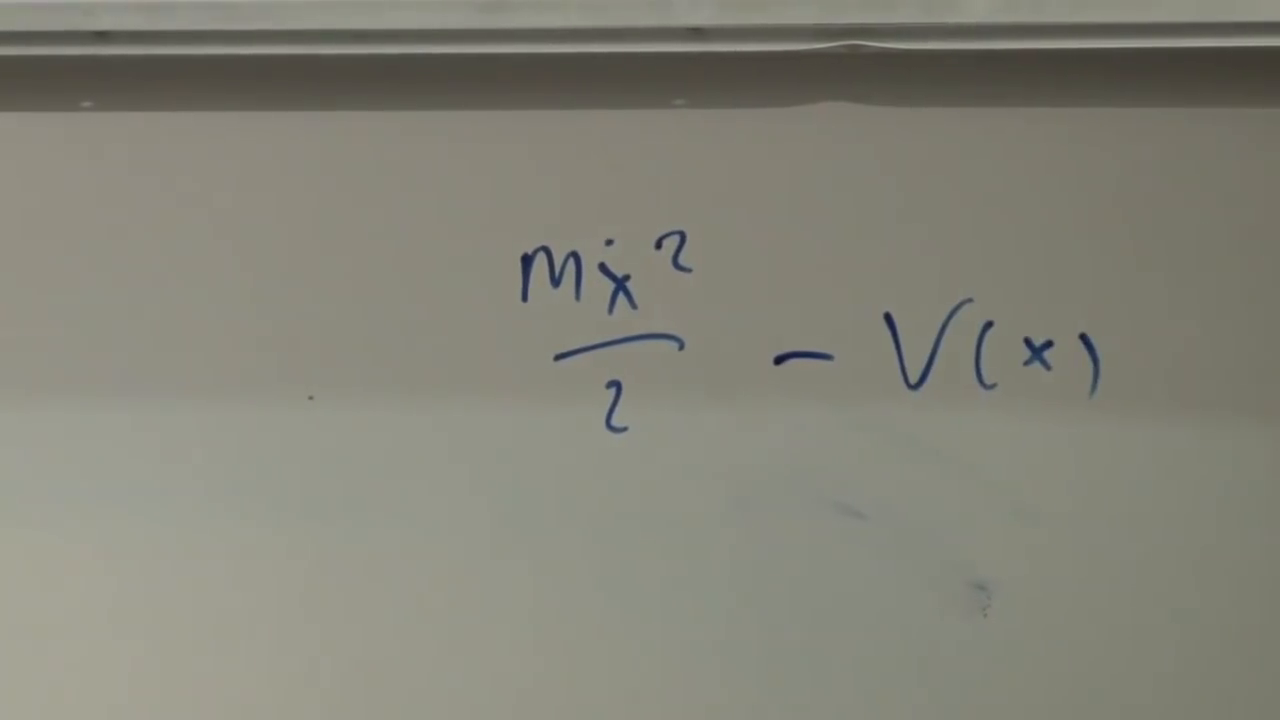
\includegraphics[width=0.72\textwidth]{lecture_04_figure_02.png}
  \caption{Die Lagrange-Funktion als kinetische minus potenzielle Energie, anhand derer der konjugierte Impuls mit \(m\dot x\) identifiziert wird.}
  \lectureframe{00:14:48}
\end{figure}

Wenn \(q_i\) in \(L\) nicht vorkommt, gilt \(\dot p_i=0\). Das ist der vertraute Weg über eine zyklische Koordinate zu einem Erhaltungssatz. Der eigentliche Zusammenhang ist allgemeiner; es ist hilfreich, ihn anhand von Beispielen zu entdecken, bevor wir ihn beweisen.

\section{Erhaltungssätze, bevor wir sie erklären}

\subsection{Zwei Koordinaten und ein nur vom Abstand abhängiges Potenzial}

Setzen wir beide Massen gleich eins und betrachten wir
\begin{equation}
  L=\frac{\dot q_1^{\,2}+\dot q_2^{\,2}}{2}-V(q_1-q_2).
  \label{eq:separation-lagrangian}
\end{equation}
Man kann sich zwei Teilchen auf einer Geraden vorstellen. Ihre Wechselwirkung hängt nur von ihrem Abstand ab.

\begin{figure}[htbp]
  \centering
  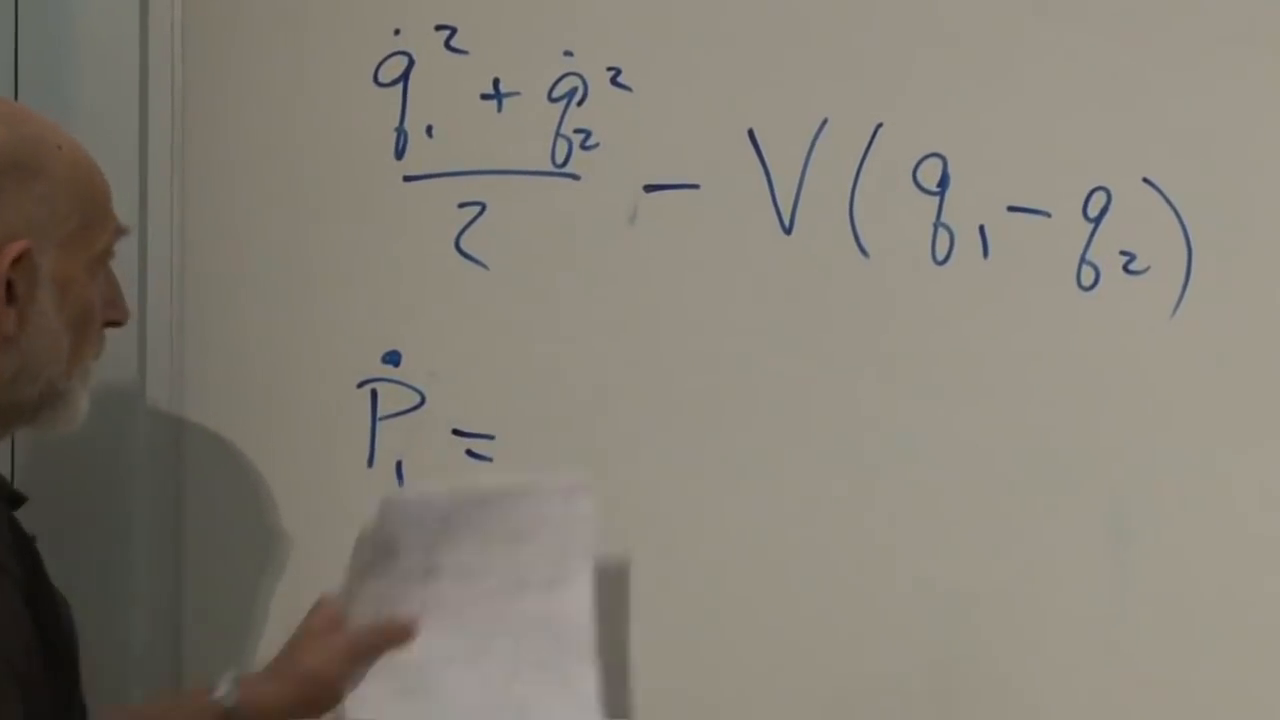
\includegraphics[width=0.78\textwidth]{lecture_04_figure_03.png}
  \caption{Die Lagrange-Funktion für zwei Koordinaten und der Beginn der ersten Impulsgleichung.}
  \lectureframe{00:18:56}
\end{figure}

Schreiben wir \(V'\) für die Ableitung nach dem Argument von \(V\), so gilt
\begin{align}
  \dot p_1&=-V'(q_1-q_2),
  \notag\\
  \dot p_2&=+V'(q_1-q_2).
  \label{eq:separation-momentum-equations}
\end{align}
Das Vorzeichen in der zweiten Gleichung kehrt sich um, weil eine Zunahme von \(q_2\) den Wert von \(q_1-q_2\) verringert.

\begin{classroomqa}
  \audiencequestion{Muss die erste Impulsgleichung \(V'\) enthalten, und woher kommt ihr Minuszeichen?
  \lecturetimestamp{00:20:52--00:21:35}}
  \lecturerresponse{Die Euler--Lagrange-Gleichung besagt
  \(\dot p_1=\partial L/\partial q_1\), nicht, dass die Lagrange-Funktion null ist.
  Da \(L=T-V\) gilt, ergibt die Ableitung nach \(q_1\) den Term
  \(-V'\). Bei der Ableitung nach \(q_2\) kommt durch \(q_1-q_2\) ein weiteres Minuszeichen hinzu, daher steht in der zweiten Gleichung \(+V'\).}
\end{classroomqa}

\begin{figure}[htbp]
  \centering
  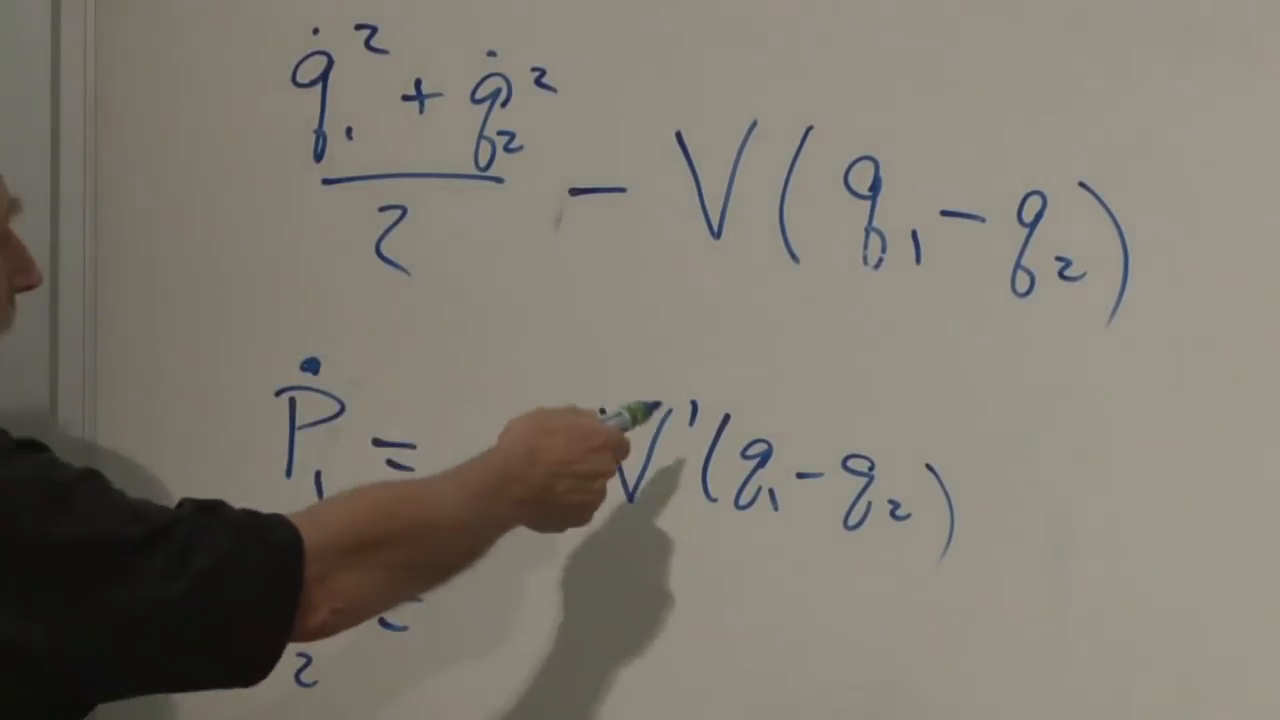
\includegraphics[width=0.78\textwidth]{lecture_04_figure_04.png}
  \caption{Die vorzeichenempfindliche Ableitung in der Gleichung für \(p_1\); in der Gleichung für \(p_2\) ergibt sich das entgegengesetzte Vorzeichen.}
  \lectureframe{00:20:41}
\end{figure}

Addiert man die Gleichungen in ~\eqref{eq:separation-momentum-equations}, erhält man
\begin{equation}
  \frac{d}{dt}(p_1+p_2)=0.
  \label{eq:total-p-conserved}
\end{equation}
Wir haben eine Erhaltungsgröße gefunden, aber noch nicht erklärt, warum sie existiert.

\subsection{Eine weniger offensichtliche Linearkombination}

Betrachten wir nun
\begin{equation}
  L=\frac{\dot q_1^{\,2}+\dot q_2^{\,2}}{2}
    -V(Aq_1+Bq_2),
  \label{eq:ab-lagrangian}
\end{equation}
wobei \(A\) und \(B\) Konstanten sind. Dann gilt
\begin{align}
  \dot p_1&=-A\,V'(Aq_1+Bq_2),
  \notag\\
  \dot p_2&=-B\,V'(Aq_1+Bq_2).
  \label{eq:ab-momentum-equations}
\end{align}
Multipliziert man die erste Gleichung mit \(B\), die zweite mit \(A\) und subtrahiert die Gleichungen, so fällt die Kraft heraus:
\begin{equation}
  \frac{d}{dt}(Bp_1-Ap_2)=0.
  \label{eq:ab-conserved}
\end{equation}

\begin{figure}[htbp]
  \centering
  \includegraphics[width=0.78\textwidth]{lecture_04_figure_06.png}
  \caption{Die gewichteten Impulsgleichungen, deren Kraftterme sich in \(Bp_1-Ap_2\) aufheben.}
  \lectureframe{00:24:20}
\end{figure}

\begin{classroomqa}
  \audiencequestion{Woher könnten Konstanten wie \(A\) und \(B\) physikalisch kommen?\lecturetimestamp{00:25:09--00:30:15}}
  \lecturerresponse{Betrachten wir zwei Teilchen mit den Massen \(m\) und \(M\):
  \[
    L=\frac{m\dot X^2}{2}+\frac{M\dot Y^2}{2}-V(X-Y).
  \]
  Skalieren wir um zu \(Q_1=\sqrt m\,X\) und \(Q_2=\sqrt M\,Y\). Der kinetische Term wird zu \((\dot Q_1^2+\dot Q_2^2)/2\), während das Potenzial von \(Q_1/\sqrt m-Q_2/\sqrt M\) abhängt. Ungleiche Massen treten somit ganz natürlich als Koeffizienten einer Linearkombination auf. Ersetzt man \(Q_2\) durch \(-Q_2\), wird aus dem dargestellten Minus ein Plus, ohne den quadrierten kinetischen Term zu verändern.}
\end{classroomqa}

\begin{figure}[htbp]
  \centering
  \includegraphics[width=0.82\textwidth]{lecture_04_figure_07.png}
  \caption{Massengewichtete Koordinaten vereinfachen die kinetische Energie und verlagern die Massenfaktoren ins Potenzial.}
  \lectureframe{00:28:40}
\end{figure}

\begin{classroomqa}
  \audiencequestion{Zeigt dies, dass eine Erhaltungsgröße auch ohne zyklische Koordinate existieren kann?\lecturetimestamp{00:31:13--00:31:58}}
  \lecturerresponse{In den hier verwendeten Variablen gibt es keine \emph{offensichtliche} zyklische Koordinate. Eine Variablentransformation könnte eine solche sichtbar machen, doch danach zu suchen, ist hier nicht der hilfreiche Blickwinkel. Das Symmetrieargument wird die erhaltene Kombination direkt identifizieren.}
\end{classroomqa}

\section{Was wir unter einer Symmetrie verstehen}

\subsection{Translationen}

Beginnen wir mit einem freien Teilchen der Masse eins,
\begin{equation}
  L=\frac{\dot q^2}{2}.
  \label{eq:free-unit-l4}
\end{equation}
und verschieben wir jeden Punkt seiner Bahn um dieselbe Konstante:
\begin{equation}
  q'(t)=q(t)+\epsilon.
  \label{eq:free-translation}
\end{equation}
Da \(\epsilon\) zeitunabhängig ist, gilt \(\dot q'=\dot q\) und somit
\(\delta L=0\). Diese Invarianz ist Translationssymmetrie.

Es gibt zwei gleichwertige Sichtweisen. Bei der passiven Beschreibung verschiebt man den Koordinatenursprung, während das Objekt an seinem Platz bleibt. Bei der aktiven Beschreibung bleiben die Achsen fest und das Objekt wird bewegt. Die aktive Ausdrucksweise ist weniger verwirrend: Wir verändern die physikalische Konfiguration und fragen, ob \(L\) davon etwas bemerkt.

Für Gl.~\eqref{eq:separation-lagrangian} verschieben wir beide Koordinaten:
\begin{equation}
  \delta q_1=\epsilon,
  \qquad
  \delta q_2=\epsilon.
  \label{eq:common-translation}
\end{equation}
Die Geschwindigkeiten bleiben unverändert, ebenso \(q_1-q_2\).

\begin{figure}[htbp]
  \centering
  \includegraphics[width=0.78\textwidth]{lecture_04_figure_08.png}
  \caption{Eine gemeinsame Translation lässt den Abstand zwischen zwei Koordinaten unverändert.}
  \lectureframe{00:35:30}
\end{figure}

Für Gl.~\eqref{eq:ab-lagrangian} verwenden wir die weniger offensichtliche Transformation
\begin{equation}
  \delta q_1=B\epsilon,
  \qquad
  \delta q_2=-A\epsilon.
  \label{eq:ab-transformation}
\end{equation}
Auch hier ändern sich die Geschwindigkeiten nicht, während
\begin{equation}
  \delta(Aq_1+Bq_2)=AB\epsilon-BA\epsilon=0.
  \label{eq:ab-invariant-argument}
\end{equation}
Damit ist diese Transformation eine Symmetrie.

\begin{figure}[htbp]
  \centering
  \includegraphics[width=0.80\textwidth]{lecture_04_figure_09.png}
  \caption{Die asymmetrische Translation, die \(Aq_1+Bq_2\) erhält.}
  \lectureframe{00:40:20}
\end{figure}

\begin{classroomqa}
  \audiencequestion{Codieren die Koeffizienten die Massen, sodass die Erhaltungsgröße zum gewöhnlichen Schwerpunktsimpuls wird?\lecturetimestamp{00:42:25--00:42:45}}
  \lecturerresponse{Ja. In den massengewichteten Variablen erscheinen die Symmetrie und die erhaltene Kombination asymmetrisch. Transformiert man zurück zu \(X\) und \(Y\), erhält man wieder die gewöhnliche gleichzeitige Translation und den Gesamtimpuls.}
\end{classroomqa}

\subsection{Rotationen}

Betrachten wir ein Teilchen in der Ebene,
\begin{equation}
  L=\frac{m}{2}(\dot x^2+\dot y^2)-V(x^2+y^2).
  \label{eq:central-lagrangian-l4}
\end{equation}
Dies ist ein Zentralpotenzial. Wir vergleichen zwei feste Koordinatensysteme, die gegeneinander gedreht sind; die Achsen rotieren nicht mit der Zeit. Bei einer konsistenten Wahl der Orientierung gilt
\begin{align}
  x'&=x\cos\theta+y\sin\theta,
  \notag\\
  y'&=-x\sin\theta+y\cos\theta.
  \label{eq:finite-rotation-l4}
\end{align}

\begin{figure}[htbp]
  \centering
  \includegraphics[width=0.82\textwidth]{lecture_04_figure_10.png}
  \caption{Eine Lagrange-Funktion für ein Zentralpotenzial und zwei feste kartesische Bezugssysteme, die durch eine Rotation miteinander verbunden sind.}
  \lectureframe{00:45:40}
\end{figure}

Setzen wir \(\theta=\epsilon\) und behalten wir nur Terme erster Ordnung:
\begin{equation}
  \cos\epsilon=1+O(\epsilon^2),
  \qquad
  \sin\epsilon=\epsilon+O(\epsilon^3).
  \label{eq:small-angle-l4}
\end{equation}
Die infinitesimale Rotation lautet
\begin{align}
  \delta x&=y\epsilon,
  &\delta y&=-x\epsilon,
  \notag\\
  \delta\dot x&=\dot y\epsilon,
  &\delta\dot y&=-\dot x\epsilon.
  \label{eq:infinitesimal-rotation-l4}
\end{align}

\begin{figure}[htbp]
  \centering
  \includegraphics[width=0.82\textwidth]{lecture_04_figure_11.png}
  \caption{Die infinitesimale Rotation der Koordinaten und Geschwindigkeiten.}
  \lectureframe{00:49:50}
\end{figure}

Anders als bei einer Translation hängt die Änderung von \(x\) von \(y\) ab; die Änderung von \(y\) wiederum hängt von \(x\) ab. Dennoch gilt
\begin{align}
  \delta(x^2+y^2)
  &=2x\,\delta x+2y\,\delta y=0,
  \notag\\
  \delta(\dot x^2+\dot y^2)
  &=2\dot x\,\delta\dot x+2\dot y\,\delta\dot y=0.
  \label{eq:rotation-invariants-l4}
\end{align}
Sowohl der Potenzialterm als auch der kinetische Term sind invariant.

\begin{figure}[htbp]
  \centering
  \includegraphics[width=0.76\textwidth]{lecture_04_figure_12.png}
  \caption{Die Aufhebung der Terme erster Ordnung zeigt, dass das Quadrat des Radius rotationsinvariant ist.}
  \lectureframe{00:53:20}
\end{figure}

\section{Der allgemeine Erhaltungssatz}

Die Beispiele der Translation und Rotation lassen sich auf dieselbe Weise darstellen. Sei eine kontinuierliche infinitesimale Transformation gegeben durch
\begin{equation}
  \delta q_i=\epsilon f_i(q),
  \qquad
  \delta\dot q_i=\frac{d}{dt}\delta q_i,
  \label{eq:general-infinitesimal-symmetry}
\end{equation}
wobei \(\epsilon\) zeitunabhängig ist und \(f_i\) von allen Koordinaten abhängen kann.

\begin{figure}[htbp]
  \centering
  \includegraphics[width=0.78\textwidth]{lecture_04_figure_13.png}
  \caption{Ein allgemeines infinitesimales Verschiebungsfeld \(\delta q_i=\epsilon f_i(q)\).}
  \lectureframe{00:56:00}
\end{figure}

Die Variation der Lagrange-Funktion erster Ordnung ist
\begin{equation}
  \delta L
  =\sum_i\left(
    \frac{\partial L}{\partial q_i}\delta q_i
    +\frac{\partial L}{\partial\dot q_i}\delta\dot q_i
  \right).
  \label{eq:delta-l-general}
\end{equation}

\begin{figure}[htbp]
  \centering
  \includegraphics[width=0.84\textwidth]{lecture_04_figure_14.png}
  \caption{Die beiden Beiträge zu \(\delta L\): Variation der Koordinaten und Variation der Geschwindigkeiten.}
  \lectureframe{01:02:30}
\end{figure}

Betrachten wir nun eine physikalische Bahn, auf der die Euler--Lagrange-Gleichungen gelten. Mit
\begin{equation}
  \frac{\partial L}{\partial\dot q_i}=p_i,
  \qquad
  \frac{\partial L}{\partial q_i}=\dot p_i,
  \label{eq:el-substitution-l4}
\end{equation}
erhalten wir
\begin{align}
  \delta L
  &=\sum_i\left(\dot p_i\,\delta q_i
                +p_i\,\delta\dot q_i\right)
  \notag\\
  &=\frac{d}{dt}\sum_i p_i\delta q_i
  =\epsilon\frac{d}{dt}\sum_i p_i f_i(q).
  \label{eq:noether-derivation-l4}
\end{align}
Der zentrale Schritt besteht lediglich in der Produktregel.

Ist die Transformation eine Symmetrie, gilt \(\delta L=0\). Da \(\epsilon\) ein beliebiger konstanter Faktor ist, folgt
\begin{equation}
  \boxed{
  \frac{d\mathcal Q}{dt}=0,
  \qquad
  \mathcal Q=\sum_i p_i f_i(q)}
  .
  \label{eq:noether-charge-l4}
\end{equation}
Dies ist der kernmechanische Teil des Satzes von Noether für exakte, zeitunabhängige Punktsymmetrien.

\begin{figure}[htbp]
  \centering
  \includegraphics[width=0.84\textwidth]{lecture_04_figure_15.png}
  \caption{Der Schritt mit der Produktregel, der die Invarianz von \(L\) in eine Erhaltungsgröße überführt.}
  \lectureframe{01:05:00}
\end{figure}

\begin{classroomqa}
  \audiencequestion{Trägt \(q\) in \(f_i(q)\) noch einen weiteren Index?
  \lecturetimestamp{01:06:57--01:07:31}}
  \lecturerresponse{Das nicht indizierte \(q\) bezeichnet die gesamte Menge
  \((q_1,q_2,\ldots)\). Jede Komponente \(f_i\) kann von all diesen
  Koordinaten abhängen. Bei einer Rotation gilt zum Beispiel \(f_x=y\) und \(f_y=-x\).}
\end{classroomqa}

Die Beispiele sind nun keine Zufälle mehr. Für eine gemeinsame Translation gilt \(f_1=f_2=1\), also
\begin{equation}
  \mathcal Q=p_1+p_2.
  \label{eq:noether-common-p}
\end{equation}
Für die asymmetrische Translation gilt \(f_1=B\), \(f_2=-A\), also
\begin{equation}
  \mathcal Q=Bp_1-Ap_2.
  \label{eq:noether-ab-p}
\end{equation}
Bei einer Rotation gilt \(f_x=y\) und \(f_y=-x\):
\begin{equation}
  \mathcal Q=p_xy-p_yx.
  \label{eq:rotation-charge-sign}
\end{equation}
Bis auf das Vorzeichen, das von der Orientierung abhängt, ist dies der Drehimpuls,
\begin{equation}
  J=xp_y-yp_x.
  \label{eq:angular-momentum-l4}
\end{equation}

\begin{figure}[htbp]
  \centering
  \includegraphics[width=0.82\textwidth]{lecture_04_figure_16.png}
  \caption{Die Noether-Ladung der Rotation, die bis auf die Orientierung dem Drehimpuls in der Ebene entspricht.}
  \lectureframe{01:11:00}
\end{figure}

Bei vielen wechselwirkenden Teilchen drehen wir alle Teilchen gemeinsam. Aufgrund der Invarianz bleibt dann die Summe ihrer Drehimpulse erhalten, nicht aber der Drehimpuls jedes einzelnen Teilchens für sich.

\section{Fragen zu den Voraussetzungen des Satzes}

\begin{classroomqa}
  \audiencequestion{Führt ein rotierendes Koordinatensystem zu einer expliziten Zeitabhängigkeit von \(\delta L\)?\lecturetimestamp{01:12:57--01:13:57}}
  \lecturerresponse{Ja. Der eben geführte Beweis setzt einen zeitunabhängigen Symmetrieparameter voraus: eine feste Translation oder eine feste Rotation. Bei einer Transformation mit zeitabhängigem Parameter treten zusätzliche Terme auf; dann ist eine allgemeinere Behandlung nötig.}
\end{classroomqa}

\begin{classroomqa}
  \audiencequestion{Bezeichnet das große \(Q\) in der Formel an der Tafel die Transformation selbst?\lecturetimestamp{01:14:02--01:15:58}}
  \lecturerresponse{Nein. Diese Notation kollidiert leider mit den Koordinaten \(q_i\). Die Transformation ist \(\delta q_i=\epsilon f_i(q)\); die daraus hervorgehende Erhaltungsgröße ist \(\mathcal Q=\sum_i p_i f_i\). Der Koeffizient \(f_i\) gibt an, wie sich die \(i\)-te Koordinate unter der Symmetrie verändert.}
\end{classroomqa}

Auch die Energieerhaltung wird durch eine Symmetrie erzeugt, aber durch eine andere: die Translation in der Zeit, also die Unabhängigkeit davon, wo der Zeitnullpunkt liegt. Dieser Fall und die Hamiltonsche Formulierung werden später behandelt.

\begin{classroomqa}
  \audiencequestion{Könnte man die tatsächliche Bewegung in ein veränderliches Koordinatensystem aufnehmen, sodass die Mechanik nur noch aus Koordinatentransformationen besteht?\lecturetimestamp{01:17:43--01:20:01}}
  \lecturerresponse{Man kann Koordinaten wählen, die einer bestimmten Bewegung folgen. Dann hängt die Transformation aber vom Anfangszustand und von der Bahn ab. Die hier verwendete Symmetrietransformation ist unabhängig davon festgelegt, welcher Lösung das System folgt. Die Bewegung selbst lässt sich natürlicher im gemeinsamen Raum der Koordinaten und Impulse darstellen.}
\end{classroomqa}

\section{Der harmonische Oszillator im Phasenraum}

Bei Masse und Federkonstante gleich eins gilt
\begin{equation}
  L=\frac{\dot q^2}{2}-\frac{q^2}{2}.
  \label{eq:oscillator-l4}
\end{equation}
Der konjugierte Impuls und die Bewegungsgleichung lauten
\begin{equation}
  p=\dot q,
  \qquad
  \dot p=-q,
  \label{eq:oscillator-first-order-l4}
\end{equation}
oder
\begin{equation}
  \dot q=p,
  \qquad
  \dot p=-q.
  \label{eq:oscillator-phase-flow}
\end{equation}
Diese Gleichungen beschreiben eine gleichförmige Kreisbewegung in der \(q\)-\(p\)-Ebene. Die Hin-und-her-Bewegung des Oszillators im Ortsraum ist die Projektion dieses Kreises auf die \(q\)-Achse: Bei \(q=0\) ist die Geschwindigkeit am größten und an den Umkehrpunkten null.

\begin{figure}[htbp]
  \centering
  \includegraphics[width=0.82\textwidth]{lecture_04_figure_17.png}
  \caption{Die Gleichungen des harmonischen Oszillators und seine Kreisbahn im \(q\)-\(p\)-Raum.}
  \lectureframe{01:25:30}
\end{figure}

\begin{classroomqa}
  \audiencequestion{Läuft die Kreisbahn im Phasenraum im Uhrzeigersinn?\lecturetimestamp{01:25:47--01:27:15}}
  \lecturerresponse{Wenn \(p\) horizontal und \(q\) vertikal aufgetragen wird, ja. Bei maximal positivem \(q\) gilt \(\dot p=-q<0\), die Bewegung weist also nach unten. Vertauscht man die Anordnung der Achsen, kehrt sich der visuelle Drehsinn um. Deshalb kann man sich die Konvention leicht falsch merken.}
\end{classroomqa}

Das Paar in Gl.~\eqref{eq:oscillator-phase-flow} ähnelt bereits den Hamilton-Gleichungen, wurde aber vollständig im Rahmen der Lagrange-Mechanik hergeleitet.

\section{Kontinuierliche und diskrete Symmetrien}

\begin{classroomqa}
  \audiencequestion{Muss eine Symmetrie durch eine infinitesimale kartesische Transformation ausgedrückt werden?\lecturetimestamp{01:27:48--01:30:31}}
  \lecturerresponse{Kartesische Koordinaten sind lediglich praktisch; für diesen Beweis ist Kontinuität die wesentliche Voraussetzung. Manche Symmetrien haben keine infinitesimale Version. Bei einem geraden Potenzial werden \(q\mapsto -q\) und \(\dot q\mapsto-\dot q\) abgebildet, wobei \(L\) unverändert bleibt. Eine Spiegelung lässt sich jedoch nicht aus beliebig kleinen Spiegelungen zusammensetzen. Diese klassische Herleitung liefert daher keine zugehörige Erhaltungsgröße.}
\end{classroomqa}

\begin{figure}[htbp]
  \centering
  \includegraphics[width=0.82\textwidth]{lecture_04_figure_18.png}
  \caption{Ein gerades Potenzial ist unter der diskreten Spiegelung \(q\mapsto -q\) invariant.}
  \lectureframe{01:29:30}
\end{figure}

\begin{classroomqa}
  \audiencequestion{Zeigt eine von null verschiedene Erhaltungsgröße \(\mathcal Q\), dass die Transformation keine Symmetrie war?\lecturetimestamp{01:30:40--01:31:30}}
  \lecturerresponse{Nein. Eine Erhaltungsgröße kann jeden beliebigen konstanten Wert haben. Entscheidend ist die Prüfung, ob \(\dot{\mathcal Q}\) gilt. Ist die aus einer vorgeschlagenen Transformation hergeleitete Größe nicht erhalten, so war diese Transformation unter den Voraussetzungen des Beweises keine Symmetrie.}
\end{classroomqa}

\begin{classroomqa}
  \audiencequestion{Die Spiegelung lässt die Lagrange-Funktion weiterhin unverändert. Warum ergibt sich daraus also kein Erhaltungssatz?\lecturetimestamp{01:31:34--01:32:27}}
  \lecturerresponse{Die Invarianz ist zwar erkennbar, doch die Herleitung führte über eine Verschiebung erster Ordnung und die Produktregel. Eine Spiegelung bringt einen mit einem einzigen diskreten Schritt von der einen Seite des Konfigurationsraums auf die andere. Ohne einen infinitesimalen Generator \(f_i\) hat die Formel \(\mathcal Q=\sum_i p_i f_i\) nichts, worauf sie angewendet werden könnte.}
\end{classroomqa}

\begin{classroomqa}
  \audiencequestion{Wie heißt die Eigenschaft, aus beliebig kleinen Transformationen aufgebaut zu sein?\lecturetimestamp{01:32:36--01:33:23}}
  \lecturerresponse{Das ist eine \emph{kontinuierliche Symmetrie}. Translation und Rotation sind kontinuierlich; die Spiegelung ist eine \emph{diskrete Symmetrie}.}
\end{classroomqa}

\begin{classroomqa}
  \audiencequestion{Können sich verworfene Fehler der Ordnung \(O(\epsilon^2)\) aufsummieren, wenn viele infinitesimale Schritte eine endliche Transformation ergeben?\lecturetimestamp{01:33:23--01:36:10}}
  \lecturerresponse{Die infinitesimale Invarianz muss an jedem Punkt gelten, der entlang der Transformation erreicht wird, nicht nur am Ausgangspunkt. Teilen wir ein endliches Parameterintervall in \(N\) Schritte der Größe \(\epsilon\) auf: Die aufsummierte Verschiebung erster Ordnung beträgt \(N\epsilon\), während sich ein lokaler Restterm der Ordnung \(O(\epsilon^2)\) zu \(N\epsilon^2=(N\epsilon)\epsilon\to0\) aufsummiert. Diese Übertragung vom Lokalen aufs Endliche wird durch kontinuierliche Transformationsgruppen formalisiert.}
\end{classroomqa}

\begin{classroomqa}
  \audiencequestion{Kommen diskrete Symmetrien in klassischen Systemen tatsächlich vor?\lecturetimestamp{01:36:32--01:37:25}}
  \lecturerresponse{Gewiss. Der harmonische Oszillator selbst besitzt das gerade Potenzial \(V(q)\propto q^2\) und ist daher unter \(q\mapsto -q\) invariant. Es gibt viele solche Beispiele; entscheidend ist nur, dass diese diskrete Invarianz keine neue klassische Noether-Ladung liefert.}
\end{classroomqa}

\begin{classroomqa}
  \audiencequestion{Wenn sowohl kontinuierliche als auch diskrete Transformationen \(L\) unverändert lassen, ist das dann nicht dieselbe Bedingung?\lecturetimestamp{01:37:37--01:39:18}}
  \lecturerresponse{Als endliche Aussage über Invarianz ist es dieselbe Bedingung, aber nicht derselbe mathematische Ausgangspunkt für diesen Beweis. Der Beweis benötigt eine Variation erster Ordnung. Bei einer Spiegelung hat der Ausdruck erste Ordnung keine Bedeutung; die Gleichungskette, die zu einer Ladung führt, lässt sich daher gar nicht erst beginnen.}
\end{classroomqa}

\begin{classroomqa}
  \audiencequestion{Wie hängt dies historisch mit dem Satz von Noether zusammen?\lecturetimestamp{01:39:26--01:40:42}}
  \lecturerresponse{Dies ist ein eingeschränkter Teil von Emmy Noethers wesentlich allgemeinerem Satz. Einzelne Zusammenhänge zwischen Symmetrien und Erhaltungsgrößen waren bereits früher bekannt, doch Noether fasste sie Anfang des zwanzigsten Jahrhunderts in einem einheitlichen und bemerkenswert allgemeinen Rahmen zusammen. Ihrer mathematischen Bedeutung wurde akademisch nicht in angemessener Weise Rechnung getragen.}
\end{classroomqa}

\begin{classroomqa}
  \audiencequestion{Ist die klassische Mechanik noch ein aktives Forschungsgebiet?\lecturetimestamp{01:40:47--01:42:37}}
  \lecturerresponse{Ja. Der hier verwendete elementare Satz ist alt, doch nichtlineare Dynamik, integrierbare Systeme, Chaos, Strömungsmechanik und geometrische Mechanik sind weiterhin lebendige Forschungsgebiete. Das Symmetrieprinzip reicht zudem weit über die klassische Teilchenmechanik hinaus.}
\end{classroomqa}

\section{Warum das Wirkungsprinzip wichtig ist}

\begin{classroomqa}
  \audiencequestion{Gibt es einen anschaulichen Grund dafür, dass Symmetrie Erhaltung zur Folge haben sollte?\lecturetimestamp{01:42:49--01:47:57}}
  \lecturerresponse{Nicht allein aufgrund der Symmetrie. Betrachten wir den viskosen Widerstand,
\[
    m\ddot x=-c\dot x.
  \]
Die Gleichung ist unter \(x\mapsto x+\epsilon\) invariant. Für \(p=m\dot x\) gilt jedoch
\[
    \dot p=-\frac{c}{m}p,
    \qquad
    p(t)=p(0)e^{-ct/m},
  \]
sodass der Impuls abnimmt. Dies ist eine effektive Gleichung für ein Teilsystem und kein fundamentales Prinzip stationärer Wirkung für \(x\) allein. Bezieht man die Flüssigkeitsmoleküle und den Rest des abgeschlossenen Systems ein, bleibt der Gesamtimpuls erhalten. Symmetrie und Erhaltung hängen über das Wirkungsprinzip der Lagrange-Mechanik zusammen, nicht allein über die Gestalt einer Differentialgleichung.}
\end{classroomqa}

\begin{figure}[htbp]
  \centering
  \includegraphics[width=0.65\textwidth]{lecture_04_figure_19.png}
  \caption{Translationsinvarianter viskoser Widerstand, bei dem der Impuls des reduzierten Teilchens dennoch abnimmt.}
  \lectureframe{01:44:30}
\end{figure}

\begin{classroomqa}
  \audiencequestion{Lässt sich quantifizieren, wann die physikalische Bahn kein Minimum der Wirkung ist?\lecturetimestamp{01:48:08--01:51:38}}
  \lecturerresponse{Ein echtes Minimum ist die Ausnahme; im Allgemeinen ist die Wirkung im Raum der Wege ein Sattel. Für den Oszillator mit Masse und Federkonstante eins gilt
  \[
    S[q]=\frac12\int(\dot q^2-q^2)\,dt.
  \]
Eine schmale, sich rasch ändernde Deformation erhöht den positiven Beitrag \(\dot q^2\). Eine breite Deformation, bei der der Weg lange Zeit leicht ausgelenkt bleibt, kann den negativen Beitrag \(-q^2\) überwiegen lassen und die Wirkung verringern. Dieselbe stationäre Bahn hat somit Richtungen, in denen die Wirkung zunimmt, und andere, in denen sie abnimmt. Die Quantenmechanik liefert durch die Sichtweise des Pfadintegrals den tieferen Ursprung der Stationarität; dieses Argument behandeln wir jedoch später.}
\end{classroomqa}

\begin{figure}[htbp]
  \centering
  \includegraphics[width=0.80\textwidth]{lecture_04_figure_20.png}
  \caption{Ein benachbarter, breit ausgelenkter Weg des Oszillators veranschaulicht, warum die stationäre Wirkung typischerweise ein Sattel und kein Minimum ist.}
  \lectureframe{01:50:20}
\end{figure}

\begin{classroomqa}
  \audiencequestion{Gibt es eine eineindeutige Zuordnung zwischen kontinuierlichen Symmetrien und Erhaltungssätzen?\lecturetimestamp{01:51:44--01:52:43}}
  \lecturerresponse{Im Rahmen der Variationsrechnung und nach Identifizierung äquivalenter oder trivialer Fälle trifft dieses Bild im Wesentlichen zu. Zu jeder kontinuierlichen Symmetrie gehört eine Ladung, und Erhaltungsgrößen lassen sich im Allgemeinen auf Symmetrien zurückführen. Präzise Formulierungen bringen technische Einschränkungen mit sich; die allgemeine Aussage sollte daher nicht unbedacht verwendet werden.}
\end{classroomqa}

\begin{classroomqa}
  \audiencequestion{Muss jede Lagrange-Funktion eine nichttriviale Symmetrie besitzen?\lecturetimestamp{01:52:43--01:53:23}}
  \lecturerresponse{Nein. Die Beispiele wurden so gewählt, dass sie Symmetrien besitzen. Eine generische Lagrange-Funktion muss unter keiner der vorgeschlagenen räumlichen Transformationen invariant sein.}
\end{classroomqa}

\begin{classroomqa}
  \audiencequestion{Sollte man eine Symmetrie letztlich als aktive Bewegung oder als passive Koordinatenänderung verstehen?\lecturetimestamp{01:53:25--01:55:08}}
  \lecturerresponse{Beide Beschreibungen lassen sich gleichwertig formulieren, doch die aktive ist hier klarer. Wir bewegen das gesamte physikalische System und fragen, ob sich die Lagrange-Funktion ändert. In der passiven Ausdrucksweise muss man stattdessen sagen, dass die \emph{Form} der Lagrange-Funktion unverändert bleibt, wenn sich das Koordinatensystem bewegt.}
\end{classroomqa}

\begin{classroomqa}
  \audiencequestion{Was kommt als Nächstes?\lecturetimestamp{01:55:10--01:55:35}}
  \lecturerresponse{Die Energieerhaltung, ihr Ursprung in der Zeittranslationssymmetrie und anschließend die Hamiltonsche Formulierung.}
\end{classroomqa}

\chapter{Energie und der Hamiltonian}

\lectureoverview{Zunächst präzisieren wir die Bedeutung einer aktiven Symmetrie und wiederholen, wie Translationen und Drehungen Impuls und Drehimpuls hervorbringen. Die noch fehlende Erhaltungsgröße ist die Energie. Die zugehörige Symmetrie ist die Translation in der Zeit; die erhaltene Größe ist der Hamiltonian \(H=\sum_i p_i\dot q_i-L\). Die Herleitung zeigt außerdem genau, wie explizite Zeitabhängigkeit Energie zwischen einem ausgewählten Teilsystem und seiner Umgebung überträgt.}

\section{Fragen vor der formalen Herleitung}

Wir nähern uns dem absoluten Minimum an klassischer Mechanik, das für die folgenden Themen erforderlich ist, auch wenn es noch viel mehr Mechanik gibt, die zu lernen sich lohnt. Noch vor Beginn der eigentlichen Herleitung kamen zwei Fragen auf.

\begin{classroomqa}\audiencequestion{Welche Bücher eignen sich im Anschluss an diesen Einführungskurs?\lecturetimestamp{00:00:36--00:02:13}}\lecturerresponse{Das etablierte fortgeschrittene Nachschlagewerk ist Herbert Goldsteins \emph{Classical Mechanics}. Auch Cornelius Lanczos’ Buch über die Variationsprinzipien der Mechanik ist eine einschlägige Quelle. Eine Leseliste für den Kurs ist hilfreicher, als so zu tun, als könne eine einzelne Lehrperson einen Überblick über alle verfügbaren Texte geben.}\end{classroomqa}

Die zweite Frage hält einen Moment in der Geschichte einer damals noch ungeklärten Messung fest. 2011 hatte das OPERA-Experiment eine scheinbar frühe Ankunft von Neutrinos gemeldet, die vom CERN zum Gran-Sasso-Labor geschickt worden waren. Die gemeldete Abweichung war kürzer als der Protonenpuls, mit dem die Neutrinos erzeugt wurden. Deshalb beruhte die Zeitmessung darauf, Pulsprofile miteinander zu vergleichen, statt ein einzelnes Neutrino beim Aussenden zu markieren und dasselbe Teilchen beim Nachweis wiederzuerkennen.

\begin{classroomqa}\audiencequestion{War das scheinbare Ergebnis, dass sich Neutrinos schneller als Licht bewegen, inzwischen geklärt?\lecturetimestamp{00:02:30--00:09:03}}\lecturerresponse{Damals ließ sich noch keine Schlussfolgerung rechtfertigen. Pulsform des Strahls, Erwärmung des Targets und Synchronisation mussten technisch genau geprüft werden. Ein spekulativer Vorschlag bezog die Bewegung eines GPS-Satelliten ein: Im Bezugssystem des Satelliten bewegen sich Quelle und Detektor, während die Zeitsignale unterwegs sind; dadurch entstehen Korrekturen in der Größenordnung einiger zehn Nanosekunden. Als Abschätzung der Größenordnung war das interessant, wurde aber nicht als glaubwürdige Erklärung des Experiments präsentiert. Die gewöhnliche Lorentz-Kontraktion bei der betreffenden Geschwindigkeit war viel zu klein, um den gemeldeten Effekt zu erklären. Die angemessene Reaktion war, die experimentelle Analyse abzuwarten.}\end{classroomqa}

\begin{figure}[htbp]\centering
  \includegraphics[width=0.78\textwidth]{lecture_05_figure_07.png}\caption{Skizze der Zeitmessung im Bezugssystem des Satelliten, die im Zusammenhang mit der historischen Frage zur Neutrinomessung besprochen wurde.}\lectureframe{00:06:30}\end{figure}

Die Diskussion der Zeitmessung wird für die folgende Mechanik nicht benötigt. Sie erinnert jedoch daran, dass eine plausible Abschätzung der Größenordnung noch keine gesicherte experimentelle Erklärung ist.

\section{Aktive Symmetrie und die Wahl des Systems}

Kehren wir zu dem Punkt zurück, der in der vorangegangenen Diskussion noch zu unklar geblieben ist: Was genau ist eine Symmetrie? Betrachten wir ein Teilchen auf einer Geraden und die Vorschrift \begin{equation}
  x\longrightarrow x+1.
  \label{eq:l5-shift-one}
\end{equation}. Es gibt zwei Möglichkeiten, sie zu verstehen. Eine \emph{passive} Transformation benennt die Punkte der Geraden um. Ein Punkt, der zuvor \(x=0\) hieß, kann nun \(x'=1\) heißen; das Teilchen hat sich dabei aber nicht bewegt. Eine \emph{aktive} Transformation lässt die Bezeichnungen unverändert und bewegt das Teilchen selbst von \(x\) nach \(x+1\). Nur die zweite Operation verändert seine Position relativ zu einem äußeren Potential.

\begin{figure}[htbp]\centering
  \includegraphics[width=0.82\textwidth]{lecture_05_figure_08.png}\caption{\(x\mapsto x+1\), die festgehaltene Koordinatengerade und ein äußeres Potential machen den Unterschied zwischen aktiver Bewegung und passiver Umbenennung deutlich.}\lectureframe{00:11:20}\end{figure}

\begin{classroomqa}\audiencequestion{Wird die Quelle des Potentials aus dem System ausgeschlossen, wenn eine Bewegung des Teilchens seine potenzielle Energie ändert?\lecturetimestamp{00:12:19--00:14:18}}\lecturerresponse{Genau. Wenn man das System als ``Teilchen in einem Potential'' bezeichnet, teilt man die Welt in das Teilchen und eine schwere Umgebung auf, etwa die Erde, die \(V(x)\) erzeugt. Die Erde erfährt zwar einen Rückstoß, doch aufgrund ihrer enormen Masse ist dieser in dieser Näherung vernachlässigbar. Eine Bewegung des Teilchens relativ zur ruhenden Erde kann \(V\) ändern; eine gemeinsame Translation von Teilchen und Erde würde das nicht tun.}\end{classroomqa}

\begin{classroomqa}\audiencequestion{Wurden im früheren Beispiel mit der Drehung auch die Geschwindigkeiten verändert, oder nur die Positionen?\lecturetimestamp{00:14:26--00:15:29}}\lecturerresponse{Ja. Eine starre aktive Drehung wirkt auf die gesamte Bewegungsgeschichte, nicht nur auf eine momentane Position. Sowohl Positionen als auch Geschwindigkeitsvektoren werden gedreht. Eine dagegen zu jedem Zeitpunkt ausgeführte konstante Translation ändert \(x\), lässt aber \(\dot x\) unverändert.}\end{classroomqa}

Der Unterschied zwischen System und Umgebung wird noch zweimal eine Rolle spielen: wenn ein zeitabhängiger Apparat Energie mit einem Teilsystem austauscht und wenn makroskopische Reibung Energie in unbeobachtbarer mikroskopischer Bewegung verbirgt.

\section{Infinitesimale Bewegungen im Konfigurationsraum}

Die Konfiguration eines allgemeinen mechanischen Systems ist ein Punkt im Raum der verallgemeinerten Koordinaten \(q_i\). Eine aktive infinitesimale Transformation bewegt jede mögliche Konfiguration in eine benachbarte. Wir schreiben \begin{equation}
  \delta q_i=\epsilon f_i(q),
  \label{eq:l5-general-transformation}
\end{equation}, wobei die Funktionen \(f_i\) ein festes Verschiebungsfeld im Konfigurationsraum festlegen. Sie können von sämtlichen Koordinaten abhängen; einige können auch verschwinden. Der gemeinsame Faktor \(\epsilon\) ist klein; er trennt die Schrittweite von der Form der Transformation.

\begin{figure}[htbp]\centering
  \includegraphics[width=0.75\textwidth]{lecture_05_figure_09.png}\caption{Ein Verschiebungsvektor, der jedem Punkt des Konfigurationsraums zugeordnet ist.}\lectureframe{00:16:50}\end{figure}

\begin{figure}[htbp]\centering
  \includegraphics[width=0.80\textwidth]{lecture_05_figure_10.png}\caption{Die koordinatenabhängige infinitesimale Transformation \(\delta q_i=\epsilon f_i(q)\).}\lectureframe{00:18:00}\end{figure}

Die Vorschrift selbst hängt nicht explizit von der Zeit ab. Ihre Wirkung auf die Geschwindigkeiten ist daher \begin{equation}
  \delta\dot q_i=\frac{d}{dt}(\delta q_i)
  =\epsilon\sum_j\frac{\partial f_i}{\partial q_j}\dot q_j.
  \label{eq:l5-velocity-variation}
\end{equation}. Bei einer Translation gilt \(f_x=1\), also \(\delta\dot x=0\). Bei einer Drehung hängt \(f_i\) von der Position ab, und die Geschwindigkeit ändert sich.

\begin{classroomqa}\audiencequestion{Ist der letzte kleine Faktor in \(\delta q_i=\epsilon f_i(q)\) an jedem Punkt dieselbe Konstante?\lecturetimestamp{00:19:58--00:20:51}}\lecturerresponse{Ja. Die einzelne Konstante \(\epsilon\) dient als Hilfsgröße, durch die alle Koordinatenänderungen von derselben kleinen Größe erster Ordnung abhängen. Die räumliche Abhängigkeit steckt in den Funktionen \(f_i(q)\), nicht in \(\epsilon\); die Funktionen müssen selbst nicht klein sein.}\end{classroomqa}

\section{Wann ist die Transformation eine Symmetrie?}

Eine aktive Transformation ändert im Allgemeinen die potenzielle Energie. Sie kann auch die kinetische Energie ändern. In krummlinigen Koordinaten hat der kinetische Term die Form \begin{equation}
  T=\frac12\sum_{i,j}g_{ij}(q)\dot q_i\dot q_j,
  \label{eq:l5-kinetic-metric}
\end{equation}, sodass sich seine Koeffizienten bei einer Bewegung im Konfigurationsraum ändern können. Der bekannte Term \(r^2\dot\theta^2\) in Polarkoordinaten ist das einfachste Beispiel dafür.

Eine Transformation ist hier eine Symmetrie, wenn sich die \emph{gesamte} Lagrangefunktion in erster Ordnung nicht ändert: \begin{equation}
  \delta L=O(\epsilon^2),
  \label{eq:l5-symmetry-condition}
\end{equation}. Dies muss an jedem Punkt des Konfigurationsraums gelten, nicht nur für die Konfiguration, die eine bestimmte Lösung gerade einnimmt.

Zum Beispiel gilt für \(x\mapsto x+\epsilon\): \begin{equation}
  \delta V=\frac{\partial V}{\partial x}\epsilon.
  \label{eq:l5-potential-variation}
\end{equation}. Verschwindet dieser Ausdruck für jedes mögliche \(x\), dann gilt \(\partial V/\partial x=0\): Das Potential ist unabhängig von \(x\). Bleibt es unter Translationen in jeder räumlichen Richtung unverändert, ist es konstant.

\begin{figure}[htbp]\centering
  \includegraphics[width=0.80\textwidth]{lecture_05_figure_11.png}\caption{\(x\)-Translation, geprüft an einem Potential \(V(y)\), das unabhängig von \(x\) ist.}\lectureframe{00:23:40}\end{figure}

Für eine glatte einparametrige Familie lässt sich aus dem Verschwinden der Änderung erster Ordnung an jedem Punkt durch Verkettung infinitesimaler Schritte eine endliche Symmetrie zusammensetzen.

\begin{classroomqa}\audiencequestion{Müssen kinetische und potenzielle Energie jeweils für sich erhalten bleiben?\lecturetimestamp{00:24:44--00:25:33}}\lecturerresponse{Nein. Invariant sein muss nur die gesamte Lagrangefunktion. Manche Lagrangefunktionen enthalten gemischte Terme aus Koordinaten-- und Geschwindigkeiten und lassen sich nicht sinnvoll in \(T\) und \(V\) aufteilen. Eine getrennte Invarianz ist dann womöglich gar keine sinnvolle Fragestellung.}\end{classroomqa}

\begin{classroomqa}\audiencequestion{Bedeutet ``keine Änderung'' eine exakt verschwindende Änderung oder nur eine, die klein genug ist, um vernachlässigt zu werden?\lecturetimestamp{00:25:34--00:28:59}}\lecturerresponse{Bei einer infinitesimalen Transformation bedeutet es, dass kein Term proportional zu \(\epsilon\) auftritt. Terme der Ordnung \(\epsilon^2\) werden in der lokalen Rechnung verworfen. Da die Bedingung erster Ordnung entlang der gesamten einparametrigen Bahn gilt, führt die Wiederholung des lokalen Schritts zur endlichen Invarianz.}\end{classroomqa}

\section{Impuls und Drehimpuls wiedergewonnen}

Für die hier betrachteten exakten, zeitunabhängigen Punktsymmetrien lautet das zuvor bewiesene Ergebnis \begin{equation}
  Q=\sum_i p_i f_i(q),
  \qquad
  p_i=\frac{\partial L}{\partial\dot q_i},
  \qquad
  \dot Q=0.
  \label{eq:l5-noether-charge}
\end{equation}. Der Faktor \(\epsilon\) gehört nicht zu \(Q\); er gibt lediglich an, wie weit wir uns entlang der Symmetriebahn bewegen.

\begin{figure}[htbp]\centering
  \includegraphics[width=0.82\textwidth]{lecture_05_figure_12.png}\caption{Die allgemeine infinitesimale Verschiebung und die zugehörige erhaltene Noether-Ladung.}\lectureframe{00:30:00}\end{figure}

Für eine Translation in \(x\) gilt \(f_x=1\) und \(Q=p_x\). Volle Translationsinvarianz führt zur Erhaltung aller drei Impulskomponenten. Bei vielen wechselwirkenden Teilchen werden alle Teilchen gemeinsam durch die Symmetrie translationiert. Daher ist \begin{equation}
  \mathbf P=\sum_a\mathbf p_a
  \label{eq:l5-total-momentum}
\end{equation} erhalten, wenn die Wechselwirkungen nur von den Relativpositionen abhängen. Ein Teilchen relativ zum Rest zu bewegen, ist keine Symmetrie.

\begin{figure}[htbp]\centering
  \includegraphics[width=0.80\textwidth]{lecture_05_figure_13.png}\caption{Eine gemeinsame Translation führt komponentenweise zur Erhaltung des Gesamtimpulses.}\lectureframe{00:32:50}\end{figure}

Für eine infinitesimale Drehung in der \(x\)-\(y\)-Ebene wählen wir die Orientierung \begin{equation}
  \delta x=-y\epsilon,
  \qquad
  \delta y=x\epsilon.
  \label{eq:l5-planar-rotation}
\end{equation}. Der Abstand vom Ursprung bleibt erhalten, denn \begin{equation}
  \delta(x^2+y^2)
  =2x\delta x+2y\delta y=0.
  \label{eq:l5-radius-invariance}
\end{equation}.

\begin{figure}[htbp]\centering
  \includegraphics[width=0.76\textwidth]{lecture_05_figure_14.png}\caption{Geometrie und Koordinatenformel einer infinitesimalen Drehung in der Ebene.}\lectureframe{00:35:05}\end{figure}

Durch Differenzieren von Gl.~\eqref{eq:l5-planar-rotation} zeigt sich, dass auch die Geschwindigkeiten gedreht werden. Daher ist \(\dot x^2+\dot y^2\) invariant, und ein Zentralpotential \(V(\sqrt{x^2+y^2})\) lässt die vollständige Lagrangefunktion unverändert. Die zugehörige Ladung ist \begin{equation}
  Q=-yp_x+xp_y=(\mathbf r\times\mathbf p)_z.
  \label{eq:l5-angular-charge}
\end{equation}.

\begin{figure}[htbp]\centering
  \includegraphics[width=0.76\textwidth]{lecture_05_figure_15.png}\caption{Die Noether-Ladung der Drehung, die \(z\)-Komponente des Drehimpulses.}\lectureframe{00:38:50}\end{figure}

Drehungen in den anderen Koordinatenebenen liefern die übrigen Komponenten. Für viele Teilchen ist der erhaltene Vektor \begin{equation}
  \mathbf J=\sum_a\mathbf r_a\times\mathbf p_a.
  \label{eq:l5-total-angular-momentum}
\end{equation}. Ein Planet im Zentralpotential eines Sterns ist das grundlegende Beispiel: Die Invarianz unter allen Drehungen impliziert die Erhaltung aller Drehimpulskomponenten.

\begin{classroomqa}\audiencequestion{Was geschieht an einer scharfen Spitze, wenn sich die Ableitung auf der einen Seite von der auf der anderen Seite unterscheidet?\lecturetimestamp{00:42:25--00:44:21}}\lecturerresponse{Das ist ein berechtigter Vorbehalt. Die vorliegende Herleitung setzt differenzierbare Funktionen mit eindeutigen Ableitungen voraus. Ein instabiles Gleichgewicht, etwa ein Körper, der auf einem glatten Maximum im Gleichgewicht gehalten wird, ist für sich genommen kein Problem: Die Ableitung existiert dort und verschwindet. Eine echte Spitze erfordert eine angepasste Behandlung.}\end{classroomqa}

\begin{classroomqa}\audiencequestion{Wenn der Transformationsparameter zeitunabhängig ist, warum ändert eine Drehung dann die Geschwindigkeiten?\lecturetimestamp{00:44:23--00:45:23}}\lecturerresponse{Der Parameter ist konstant, aber das Verschiebungsfeld hängt von den Koordinaten ab. Die allgemeine Vorschrift lautet \(\delta\dot q_i=d(\delta q_i)/dt\). Bei einer Translation ist \(\delta x\) konstant, wohingegen bei einer Drehung \(\delta x=-y\epsilon\) gilt und daher \(\delta\dot x=-\dot y\epsilon\).}\end{classroomqa}

\section{Über die elementare Form „kinetische minus potenzielle Energie“ hinaus}

Für gewöhnliche nichtrelativistische Teilchen in kartesischen Koordinaten und ohne Magnetfelder gilt \(L=T-V\). Allgemeinere Koordinaten führen zur quadratischen Form aus Gl.~\eqref{eq:l5-kinetic-metric}. Ein Magnetfeld bringt einen linearen Term in der Geschwindigkeit mit sich, schematisch \(\mathbf A(q)\cdot\dot{\mathbf q}\), der Koordinaten und Geschwindigkeiten miteinander verknüpft. In einem solchen Fall ist es besser, \(L(q,\dot q,t)\) als eine einzige Funktion zu behandeln, statt jeden Term gewaltsam einer der üblichen Kategorien kinetische oder potenzielle Energie zuzuordnen.

\begin{figure}[htbp]\centering
  \includegraphics[width=0.80\textwidth]{lecture_05_figure_16.png}\caption{Ein allgemeiner koordinatenabhängiger quadratischer kinetischer Term neben einem nur von den Koordinaten abhängigen Potential.}\lectureframe{00:47:20}\end{figure}

\begin{classroomqa}\audiencequestion{Warum lässt sich eine Lagrangefunktion möglicherweise nicht sauber in kinetische und potenzielle Energie zerlegen, und ist sie trotzdem als \(T-V\) definiert?\lecturetimestamp{00:45:26--00:48:13}}\lecturerresponse{Das kann an krummlinigen Koordinaten oder an echten geschwindigkeitsabhängigen Wechselwirkungen wie dem Magnetismus liegen. Nur wenn die Lagrangefunktion aus einer quadratischen Form der Geschwindigkeiten minus einer ausschließlich koordinatenabhängigen Funktion besteht, bezeichnen wir diese Teile als \(T\) und \(V\). Andernfalls bleibt die Lagrangefunktion eine vollkommen zulässige Funktion von \(q\) und \(\dot q\), aber die Aufteilung ist nicht hilfreich. Die korrekte allgemeine Definition der Energie wird sich aus dem Hamiltonian ergeben.}\end{classroomqa}

\begin{classroomqa}\audiencequestion{War das Beispiel mit der hängenden Kette aus der ersten Sitzung eine Anwendung des Prinzips der kleinsten Wirkung?\lecturetimestamp{00:48:15--00:49:45}}\lecturerresponse{Es war ein Gleichgewichtsproblem, das dem Prinzip der kleinsten Energie folgt, und keine durch stationäre Wirkung ausgewählte Bewegungsgeschichte. Für eine statische Lösung eines gewöhnlichen Systems der Form \(T-V\) gilt \(\dot p_i=0\), und die Euler---Lagrange-Gleichung reduziert sich auf \(\partial V/\partial q_i=0\), die Bedingung dafür, dass das Potential einen stationären Punkt hat.}\end{classroomqa}

Impuls und Drehimpuls sind nun mit räumlichen Symmetrien verknüpft. Die auffällig fehlende Größe ist die Energie.

\section{Translationsinvarianz in der Zeit}

Stellen wir uns ein Experiment vor, das bei \(t_0\) beginnt, bei \(t_1\) endet und ein Ergebnis liefert. Wiederholen wir dieselbe Präparation später, mit Beginn bei \(t_0+\Delta t\) und Ende bei \(t_1+\Delta t\). Bleibt das Ergebnis unverändert, ist das System unter einer aktiven Translation in der Zeit invariant.

\begin{figure}[htbp]\centering
  \includegraphics[width=0.82\textwidth]{lecture_05_figure_17.png}\caption{Ein Experiment und seine zeitlich verschobene Kopie im Konfigurationsraum der Bewegungsgeschichte.}\lectureframe{00:52:45}\end{figure}

Ein geladenes Teilchen zwischen Kondensatorplatten veranschaulicht das Versagen dieser Symmetrie. Bei fester Ladung auf den Platten lässt sich dasselbe Experiment zu jedem beliebigen Zeitpunkt durchführen. Lädt ein äußerer Generator die Platten fortlaufend auf, sieht das Teilchen je nach Freisetzungszeit ein anderes elektrisches Feld. Das Teilchen ist dann ein explizit angetriebenes Teilsystem.

\begin{figure}[htbp]\centering
  \includegraphics[width=0.82\textwidth]{lecture_05_figure_18.png}\caption{Feste und sich äußerlich verändernde Kondensatorplatten im Vergleich, neben der Darstellung der Zeittranslation.}\lectureframe{00:54:45}\end{figure}

Derselbe Punkt zeigt sich bei einem Oszillator: \begin{equation}
  L=\frac12m\dot x^2-\frac12k(t)x^2.
  \label{eq:l5-driven-oscillator}
\end{equation}. Ein äußeres elektrisches oder magnetisches Feld könnte das Material langsam verändern und damit auch seine effektive Federkonstante. Wenn \(k\) variiert, ändert sich das Ergebnis, sobald man das Oszillatorexperiment zeitlich verschiebt.

\begin{figure}[htbp]\centering
  \includegraphics[width=0.78\textwidth]{lecture_05_figure_19.png}\caption{Kinetische und potenzielle Terme des Oszillators bei der Diskussion einer zeitabhängigen Federkonstante.}\lectureframe{00:56:45}\end{figure}

Nimmt man den Apparat, der \(k\) verändert, in das System auf, lässt sich das gesamte abgeschlossene Experiment wieder zeitlich verschieben, und seine Gesamtenergie bleibt erhalten. Die scheinbare Nichterhaltung ist ein Energieaustausch über eine von uns gewählte Systemgrenze.

In der Pause wurde der kleine Transformationsparameter in \(\epsilon\) umbenannt, um den optisch verwirrenden Ausdruck \(\delta x=\delta\) zu vermeiden. Außerdem wurde für die gemeinsame Leseliste ein Buch über Emmy Noether empfohlen.

\begin{classroomqa}\audiencequestion{Wenn die Lagrangefunktion nicht als \(T-V\) vorgegeben ist, woher stammt sie dann?\lecturetimestamp{01:00:17--01:02:24}}\lecturerresponse{Sie lässt sich aus Experimenten erschließen, aus bekannten Bewegungsgleichungen rekonstruieren, aufgrund von Symmetrie und anderen theoretischen Prinzipien vermuten oder durch Ausprobieren finden. Sobald \(L(q,\dot q,t)\) gegeben ist, führt die Euler---Lagrange-Rechnung zu den Bewegungsgleichungen. Die formale Herleitung setzt nicht voraus, dass wir zuerst den Ursprung der Lagrangefunktion klären.}\end{classroomqa}

Die operationale Prüfung auf Zeittranslationsinvarianz ist nun unmittelbar. Reichen die Kenntnis von \(q\) und \(\dot q\) aus, um \(L\) zu bestimmen, ohne zusätzlich die Uhrzeit kennen zu müssen, dann gilt \begin{equation}
  \frac{\partial L}{\partial t}=0.
  \label{eq:l5-no-explicit-time}
\end{equation}. Das besagt nicht, dass \(L(q(t),\dot q(t))\) während einer Bewegung konstant ist. Es besagt nur, dass es keine Zeitabhängigkeit gibt, die über diejenige hinausgeht, die durch die sich entwickelnden Koordinaten und Geschwindigkeiten vermittelt wird.

Ein rotierendes schweres Hantelmodell ist ein weiteres Beispiel für ein angetriebenes System. Erzeugt seine vorgegebene Bewegung für ein leichtes Probeteilchen ein zeitlich veränderliches Gravitationspotential, so hängt die Lagrangefunktion des Probeteilchens explizit von der Zeit ab. Behandelte man die Hantel stattdessen dynamisch, würde man das System erweitern und diese äußere Zeitabhängigkeit beseitigen.

\begin{figure}[htbp]\centering
  \includegraphics[width=0.80\textwidth]{lecture_05_figure_20.png}\caption{Eine vorgegebene rotierende Hantel wirkt als zeitabhängige äußere Quelle auf ein leichteres Teilchen.}\lectureframe{01:06:25}\end{figure}

\section{Herleitung des Hamiltonians}

Nehmen wir an, wir wüssten nichts über die Formel für die Energie und vermuteten, dass vielleicht die Lagrangefunktion selbst erhalten ist. Das lässt sich direkt prüfen, indem man sie entlang einer tatsächlichen Bahn ableitet. Beginnen wir der Einfachheit halber ohne explizite Zeitabhängigkeit: \begin{equation}
  \frac{dL}{dt}
  =\sum_i\left(
    \frac{\partial L}{\partial q_i}\dot q_i
    +\frac{\partial L}{\partial\dot q_i}\ddot q_i
  \right).
  \label{eq:l5-chain-rule-no-time}
\end{equation}

\begin{figure}[htbp]\centering
  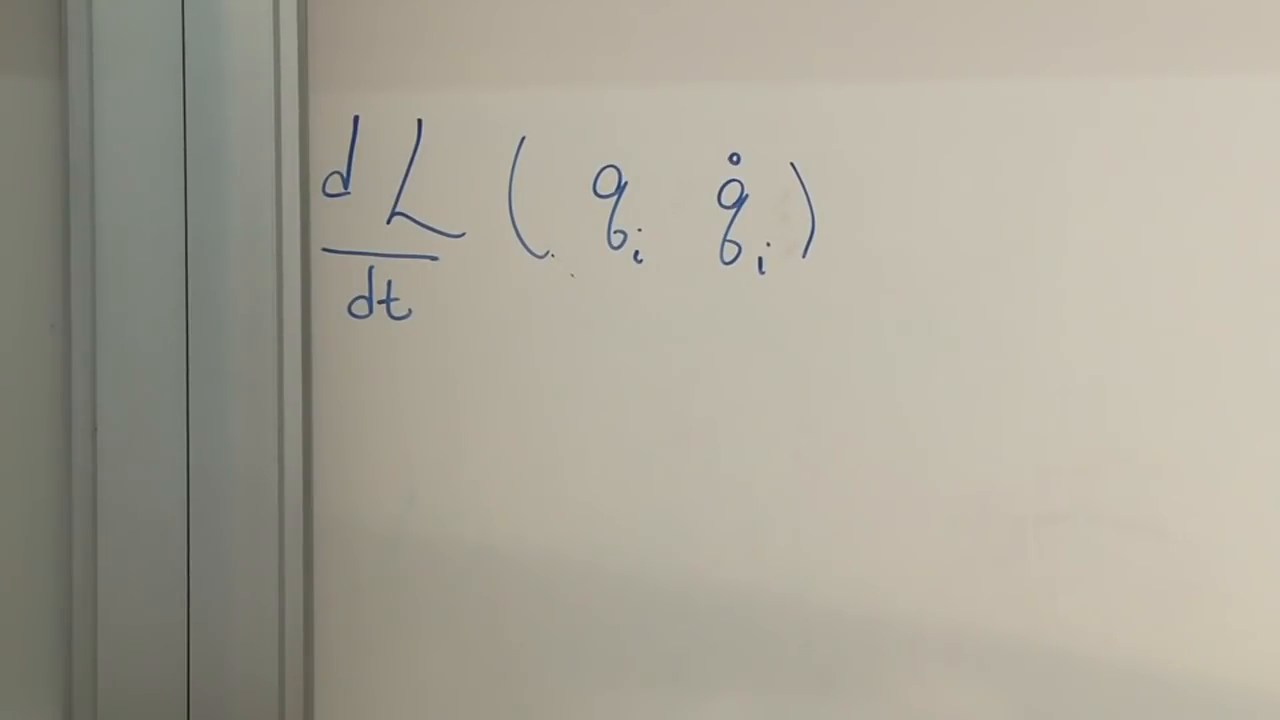
\includegraphics[width=0.72\textwidth]{lecture_05_figure_02.png}\caption{Beginn der Ableitung von \(L(q_i,\dot q_i)\) entlang der Bahn.}\lectureframe{01:08:51}\end{figure}

\begin{classroomqa}\audiencequestion{Fehlt in dem Ausdruck für die Kettenregel eine Summe?\lecturetimestamp{01:10:39--01:11:05}}\lecturerresponse{Ja. Jede Koordinate und jede Geschwindigkeit kann die Lagrangefunktion ändern, also werden beide Terme über \(i\) summiert.}\end{classroomqa}

Verwenden wir den kanonischen Impuls und die Euler---Lagrange-Gleichung: \begin{equation}
  p_i=\frac{\partial L}{\partial\dot q_i},
  \qquad
  \dot p_i=\frac{\partial L}{\partial q_i}.
  \label{eq:l5-p-and-pdot}
\end{equation}. Dann wird Gl.~\eqref{eq:l5-chain-rule-no-time} zu \begin{align}
  \frac{dL}{dt}
  &=\sum_i(\dot p_i\dot q_i+p_i\ddot q_i)
  \notag\\
  &=\frac{d}{dt}\sum_i p_i\dot q_i.
  \label{eq:l5-product-rule}
\end{align}. Der ``Trick'' besteht lediglich in der Produktregel.

\begin{figure}[htbp]\centering
  \includegraphics[width=0.84\textwidth]{lecture_05_figure_21.png}\caption{Die Kettenregel wird mithilfe der Bewegungsgleichungen zur Ableitung von \(\sum_i p_i\dot q_i\).}\lectureframe{01:13:45}\end{figure}

\begin{classroomqa}\audiencequestion{Muss im letzten Produkt \(q_i\) einmal oder zweimal punktiert sein?\lecturetimestamp{01:14:31--01:15:32}}\lecturerresponse{Im Produkt steht \(p_i\dot q_i\) mit einem Punkt. Beim Ableiten des Produkts ergibt sich \(\dot p_i\dot q_i+p_i\ddot q_i\); daher treten im ausmultiplizierten zweiten Term zwei Punkte auf.}\end{classroomqa}

Durch Subtraktion der beiden Ableitungen erhält man eine erhaltene Kombination. Der historischen Konvention folgend wählen wir ihr Negatives und nennen es den Hamiltonian: \begin{equation}
  H=\sum_i p_i\dot q_i-L.
  \label{eq:l5-hamiltonian-definition}
\end{equation}

\begin{figure}[htbp]\centering
  \includegraphics[width=0.80\textwidth]{lecture_05_figure_22.png}\caption{Die erhaltene Kombination \(L-\sum_i p_i\dot q_i=-H\) und die Definition des Hamiltonians.}\lectureframe{01:18:05}\end{figure}

Für ein Teilchen in einem Potential gilt \begin{equation}
  L=\frac12m\dot x^2-V(x),
  \qquad p=m\dot x.
  \label{eq:l5-particle-lagrangian}
\end{equation}. Daher \begin{align}
  H&=p\dot x-L
  \notag\\
   &=m\dot x^2-\left(\frac12m\dot x^2-V(x)\right)
  \notag\\
   &=\frac12m\dot x^2+V(x)=T+V.
  \label{eq:l5-particle-energy}
\end{align}.

\begin{figure}[htbp]\centering
  \includegraphics[width=0.86\textwidth]{lecture_05_figure_23.png}\caption{Der Hamiltonian eines Teilchens in einem Potential reduziert sich auf die bekannte Summe aus kinetischer und potenzieller Energie.}\lectureframe{01:20:50}\end{figure}

Bei der Herleitung wurde keine bestimmte Form von \(L\) vorausgesetzt. Daher ist Gl.~\eqref{eq:l5-hamiltonian-definition}, nicht \(T+V\), in diesem Formalismus die allgemeine Definition der Energie.

\section{Explizite Zeitabhängigkeit und Energieaustausch}

Nehmen wir die explizite Zeitabhängigkeit wieder in die Kettenregel auf: \begin{equation}
  \frac{dL}{dt}
  =\sum_i\left(
    \frac{\partial L}{\partial q_i}\dot q_i
    +\frac{\partial L}{\partial\dot q_i}\ddot q_i
  \right)
  +\frac{\partial L}{\partial t}.
  \label{eq:l5-full-chain-rule}
\end{equation}. Die linke Seite ist die totale Ableitung entlang der Bewegung. Bei der letzten partiellen Ableitung werden \(q\) und \(\dot q\) konstant gehalten; sie berücksichtigt nur Parameter, die sich aufgrund äußerer Einflüsse ändern. Wiederholen wir denselben Schritt mit der Produktregel, ergibt sich \begin{equation}
  \boxed{\frac{dH}{dt}=-\frac{\partial L}{\partial t}}.
  \label{eq:l5-hamiltonian-time}
\end{equation}.

\begin{figure}[htbp]\centering
  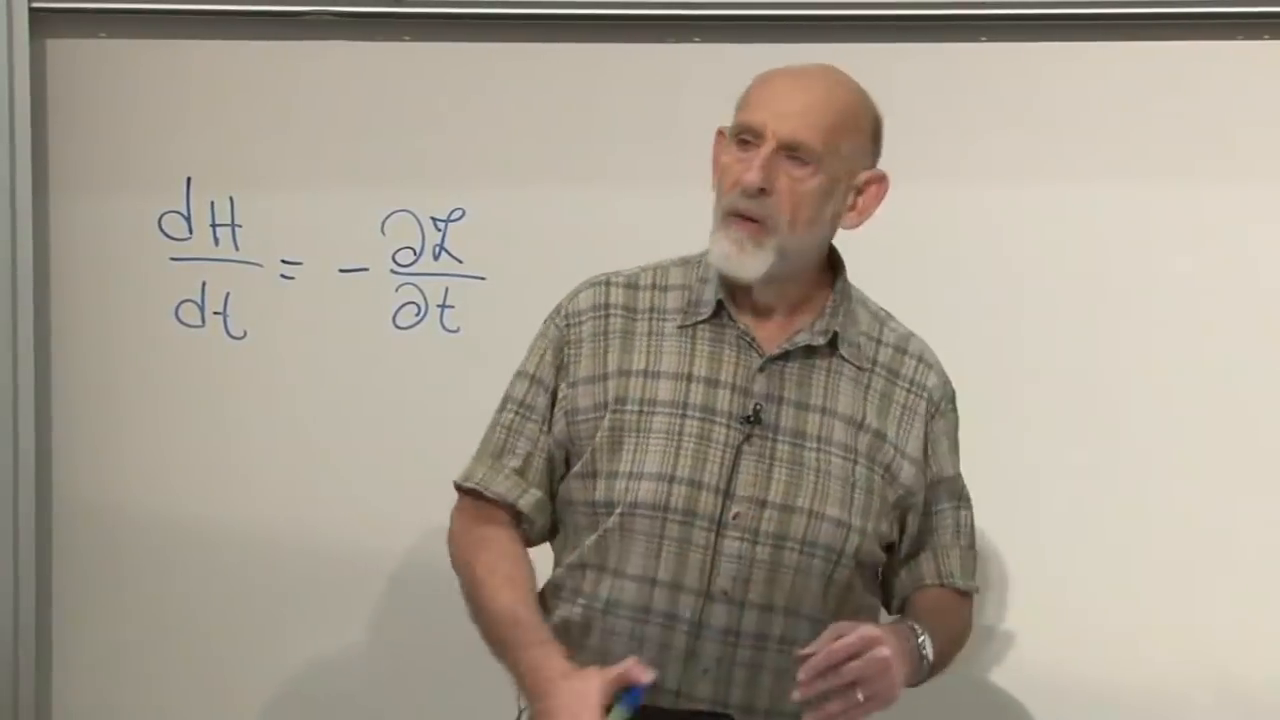
\includegraphics[width=0.70\textwidth]{lecture_05_figure_04.png}\caption{Der Hamiltonian ändert sich nur aufgrund der expliziten Zeitabhängigkeit der Lagrangefunktion.}\lectureframe{01:37:22}\end{figure}

Für den angetriebenen Oszillator aus Gl.~\eqref{eq:l5-driven-oscillator} gilt \begin{equation}
  \frac{\partial L}{\partial t}
  =-\frac12\dot k(t)x^2,
  \qquad
  \dot H=\frac12\dot k(t)x^2.
  \label{eq:l5-driven-energy-rate}
\end{equation}. Bei \(x=0\) verschwindet die momentane Änderungsrate; außerhalb des Ursprungs leistet die Änderung der Federkonstante Arbeit mit einer Rate proportional zu \(x^2\dot k\).

\begin{classroomqa}\audiencequestion{Wenn die Energie nicht erhalten ist, ist ihre Definition dann die Zeitableitung des Hamiltonians?\lecturetimestamp{01:27:11--01:28:04}}\lecturerresponse{Nein. Die Energie ist \(H\). Ihre Ableitung sagt uns, wie sich diese Energie ändert. Hat die Lagrangefunktion die vertraute Form, gilt \(H=T+V\); andernfalls liefert Gl.~\eqref{eq:l5-hamiltonian-definition} die Definition. Erweitert man das System um den äußeren Antrieb, ist der gesamte Hamiltonian wieder erhalten.}\end{classroomqa}

\begin{classroomqa}\audiencequestion{Wie lässt sich das auf die frühere Beobachterin auf einem rotierenden Karussell anwenden, bei der Zentrifugal- und Coriolisterme auftraten?\lecturetimestamp{01:28:08--01:29:52}}\lecturerresponse{Ein gleichmäßig rotierendes Koordinatensystem ist eine zeitabhängige Variablentransformation, keine feste räumliche Symmetrie und auch keine einfache Translation in der Zeit. Aus der transformierten Lagrangefunktion lässt sich ein Hamiltonian konstruieren. Diese gesonderte Rechnung sollte jedoch am besten aufgeschoben werden, bis wir Magnetkräfte behandeln, da die Algebra eine eng verwandte Form hat.}\end{classroomqa}

\section{Der Werkzeugkasten der Lagrange-Mechanik auf einen Blick}

Die gesamte Struktur lässt sich nun kompakt zusammenfassen: \begin{align}
  L&=L(q_i,\dot q_i,t),
  \notag\\
  p_i&=\frac{\partial L}{\partial\dot q_i},
  \qquad
  \dot p_i=\frac{\partial L}{\partial q_i},
  \notag\\
  \delta q_i&=\epsilon f_i(q)
  \quad\Longrightarrow\quad
  Q=\sum_i p_i f_i(q),\quad \dot Q=0,
  \notag\\
  H&=\sum_i p_i\dot q_i-L,
  \qquad
  \dot H=-\frac{\partial L}{\partial t}.
  \label{eq:l5-toolkit}
\end{align}

\begin{figure}[htbp]\centering
  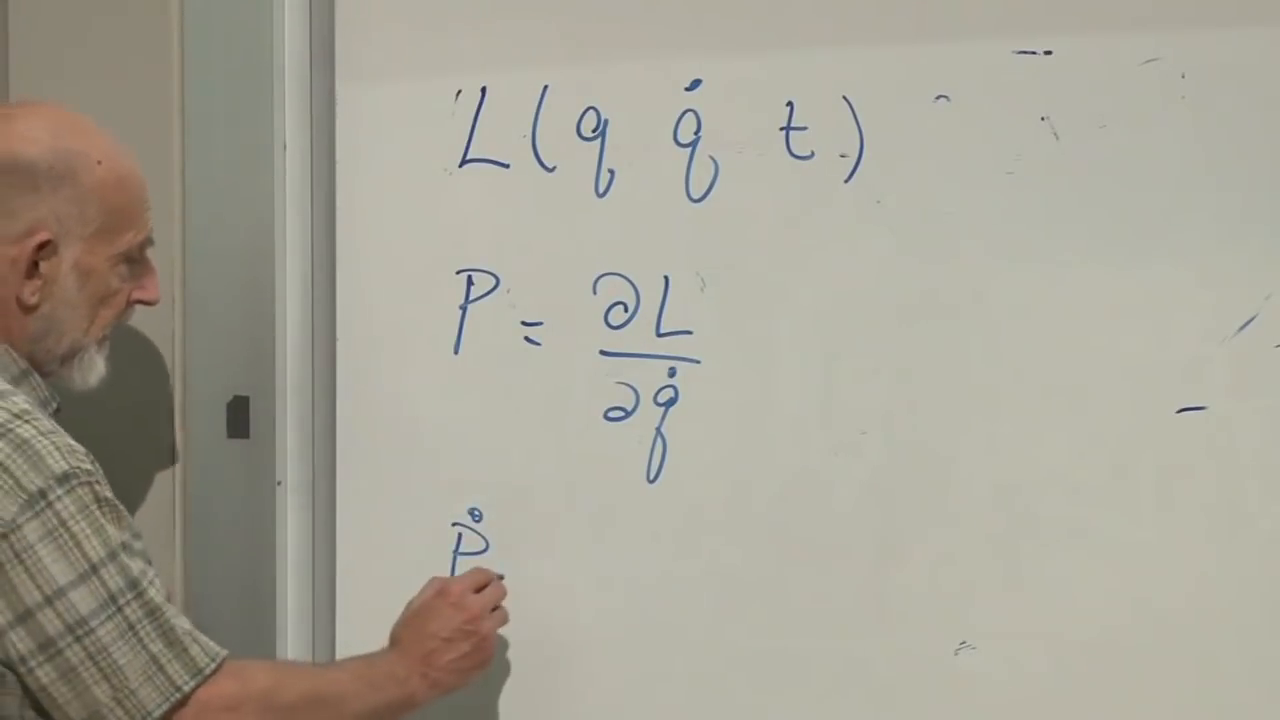
\includegraphics[width=0.66\textwidth]{lecture_05_figure_03.png}\caption{Die Zusammenfassung an der Tafel beginnt mit \(L(q,\dot q,t)\), dem kanonischen Impuls und der Euler---Lagrange-Gleichung.}\lectureframe{01:31:37}\end{figure}

Diese Formeln umfassen eine Definition, Bewegungsgleichungen, die Ladung einer gewöhnlichen kontinuierlichen Symmetrie und die Ladung der Zeittranslation. Es gibt nur wenige Kniffe; entscheidend ist, die Formeln herleiten zu können, statt voneinander losgelöste Ausdrücke auswendig zu lernen.

\section{Wozu dient die Lagrange- oder Hamilton-Mechanik?}

\begin{classroomqa}\audiencequestion{Lässt sich die Mechanik gleichwertig mit \(L\) oder \(H\) beschreiben, und warum entscheidet man sich für die eine oder andere Formulierung?\lecturetimestamp{01:37:16--01:39:18}}\lecturerresponse{Bei regulärer Legendre-Transformation sind sie äquivalent, doch sie heben unterschiedliche Strukturen hervor. Die Lagrange-Mechanik geht auf natürliche Weise von stationärer Wirkung aus. Die Hamilton-Mechanik ist zunächst abstrakter, doch ihre Gleichungen sind einfach, und sie wird in der Quantenmechanik zentral. Der Hamiltonian ist die Energie, seine Bedeutung geht aber weit über das Energieerhaltungsgesetz hinaus.}\end{classroomqa}

\begin{classroomqa}\audiencequestion{Kannte Newton die Hamiltonsche Form der Energieerhaltung?\lecturetimestamp{01:39:29--01:39:56}}\lecturerresponse{Soweit aus den historischen Quellen hervorgeht, nicht in dieser Formulierung. Newtons ausdrücklich angegebener Rahmen war das Kraftgesetz \(F=ma\).}\end{classroomqa}

\begin{classroomqa}\audiencequestion{Warum sollte jedes physikalische System eine Lagrangefunktion besitzen? Ist das lediglich eine experimentelle Tatsache?\lecturetimestamp{01:39:57--01:42:37}}\lecturerresponse{Für die hier betrachteten abgeschlossenen Systeme ist es eine empirische Tatsache und folgt außerdem aus der tiefer liegenden Quantenbeschreibung. Mathematisch konsistente Differentialgleichungen lassen sich angeben, die keine Euler---Lagrange-Gleichungen sind. Zum Beispiel ist \(\dot x=-x\) problemlos lösbar, doch als fundamentales Gesetz für ein abgeschlossenes System mit einer Koordinate hat es den informationsvernichtenden Charakter einer Dissipation. Die klassische Mechanik geht der Quantenmechanik logisch nicht voraus; ihre fundamentale Struktur ist von der Quantenmechanik übernommen. Der genaue Grund muss noch warten.}\end{classroomqa}

\begin{classroomqa}\audiencequestion{Wenn jedes reale abgeschlossene System eine Lagrangefunktion hat, entspricht dann jede Funktion, die wir Lagrangefunktion nennen, einem in der Natur vorkommenden System?\lecturetimestamp{01:42:39--01:42:54}}\lecturerresponse{Nein. Der formale Kalkül lässt viele Funktionen zu, die durch kein bekanntes physikalisches System verwirklicht werden.}\end{classroomqa}

\begin{classroomqa}\audiencequestion{Ist die Lagrangefunktion vor allem ein Werkzeug, um Potentiale zu erfinden?\lecturetimestamp{01:42:54--01:43:32}}\lecturerresponse{Sie ist vielseitiger. Mit ihr lassen sich mögliche mechanische Systeme ordnen; außerdem ist sie häufig der kürzeste praktikable Weg zu den Bewegungsgleichungen.}\end{classroomqa}

Das Doppelpendel veranschaulicht diesen praktischen Vorteil. Wählen wir zwei Winkel, berechnen wir die Geschwindigkeiten beider Massen anhand dieser Winkel und ihrer Zeitableitungen, bilden wir \(T-V\) und überlassen die implizite Berücksichtigung der Zwangskräfte den Euler---Lagrange-Gleichungen. Das ist deutlich übersichtlicher, als sämtliche Spannkräfte und Beschleunigungen mit \(F=ma\) zu bestimmen.

\begin{figure}[htbp]\centering
  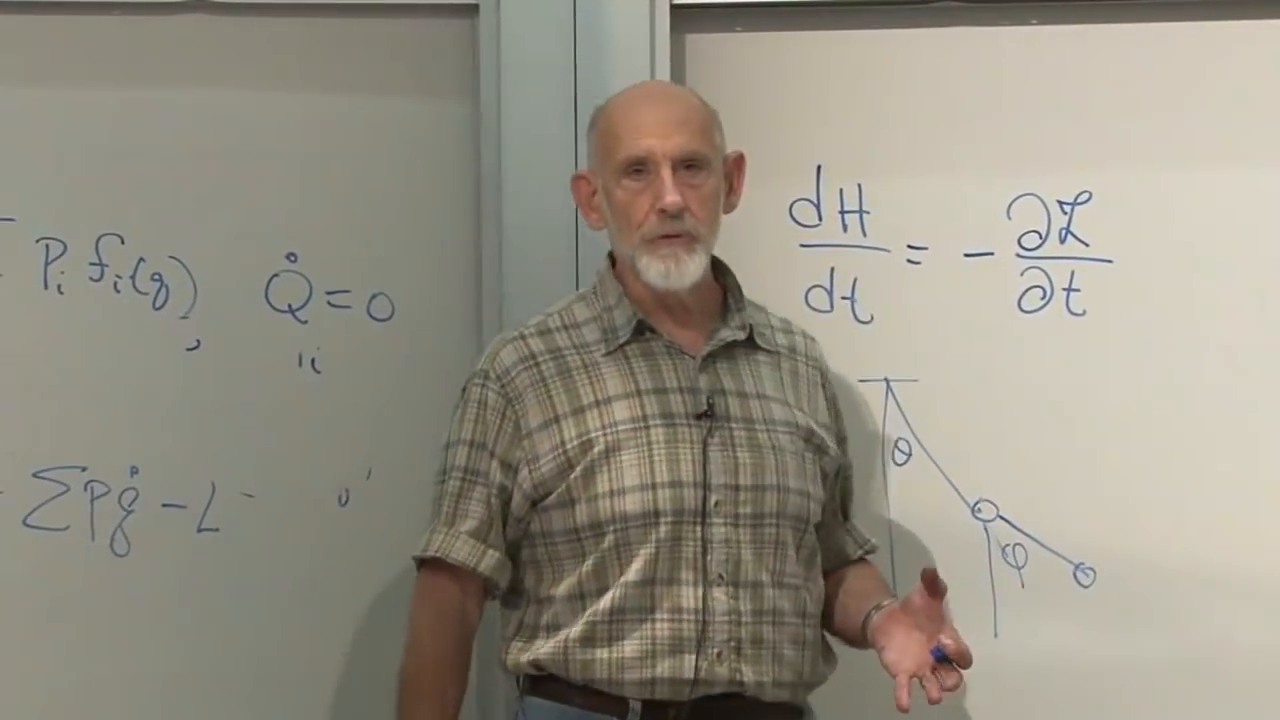
\includegraphics[width=0.84\textwidth]{lecture_05_figure_05.png}\caption{Die Identität für die Änderungsrate der Energie bleibt neben der Skizze des Doppelpendels an der Tafel stehen.}\lectureframe{01:45:39}\end{figure}

\begin{figure}[htbp]\centering
  \begin{tikzpicture}[scale=1.15]
    \draw[thick] (-0.5,0) -- (0.5,0);
    \fill (0,0) circle (0.045);
    \draw[dashed] (0,0) -- (0,-2.3);
    \draw[thick] (0,0) -- (-0.92,-1.22);
    \fill (-0.92,-1.22) circle (0.07);
    \draw[dashed] (-0.92,-1.22) -- (-0.92,-2.55);
    \draw[thick] (-0.92,-1.22) -- (-0.25,-2.18);
    \fill (-0.25,-2.18) circle (0.07);
    \draw (0,-0.55) arc (-90:-127:0.55);
    \node at (-0.42,-0.56) {$\theta$};
    \draw (-0.92,-1.72) arc (-90:-55:0.48);
    \node at (-0.56,-1.72) {$\phi$};
  \end{tikzpicture}\caption{Verallgemeinerte Winkelkoordinaten für ein Doppelpendel.}\end{figure}

Auch ein Variablenwechsel ist effizient: Man transformiert eine Lagrangefunktion und leitet anschließend ihre Bewegungsgleichungen her, statt jede Kraftgleichung einzeln zu transformieren.

\begin{classroomqa}
  \audiencequestion{Ist das Doppelpendel im Wesentlichen ein weiteres Dreikörpersystem, etwa Sonne, Erde und Mond, bei dem ein Körper als Bezugspunkt behandelt wird?
  \lecturetimestamp{01:45:06--01:45:25}}
  \lecturerresponse{Diese Analogie erfasst die Hierarchie, auch wenn die Stäbe andere Zwangsbedingungen auferlegen. In beiden Fällen kann man in einer Näherung einen sehr massereichen oder festgehaltenen Bestandteil als Bezugsstruktur behandeln.}
\end{classroomqa}

\begin{classroomqa}
  \audiencequestion{Beim Doppelpendel verwendet man \(T-V\), obwohl gerade allgemeinere Lagrangefunktionen behandelt wurden. Wann ist \(T-V\) gültig?
  \lecturetimestamp{01:46:08--01:46:58}}
  \lecturerresponse{Für gewöhnliche nichtrelativistische Teilchen in einem Inertialsystem, bei denen keine magnetische Geschwindigkeitskopplung vorliegt, gilt die bekannte Form. Rotierende Bezugssysteme, relativistische Systeme und Magnetfelder erfordern allgemeinere Terme.}
\end{classroomqa}

\begin{classroomqa}
  \audiencequestion{Liegen Stöße außerhalb dieser Beschreibung?
  \lecturetimestamp{01:47:00--01:48:05}}
  \lecturerresponse{Elastische Stöße entstehen durch kurzreichweitige Kräfte und damit durch Potenziale. Inelastische Stöße sind auf mikroskopischer Ebene weiterhin mechanisch, doch Energie geht in innere Schwingungen, Verformung und Wärme über. Eine Beschreibung des Schwerpunkts, die diese Freiheitsgrade auslässt, ist unvollständig.}
\end{classroomqa}

\begin{classroomqa}
  \audiencequestion{Lässt sich ein Baseball, der von einem Schläger getroffen wird, mit \(F=ma\) analysieren?
  \lecturetimestamp{01:48:05--01:48:33}}
  \lecturerresponse{Nur in einer groben Beschreibung. Eine vollständige Behandlung muss Verformung, Erwärmung, mögliche Schäden am Ball und vielleicht auch einen zerbrechenden Schläger berücksichtigen. Diese inneren Freiheitsgrade machen einen realistischen Aufprall viel schwieriger als einen Stoß von Punktteilchen.}
\end{classroomqa}

\begin{classroomqa}
  \audiencequestion{Wie steht es mit einem ausgedehnten starren Körper?
  \lecturetimestamp{01:48:34--01:49:00}}
  \lecturerresponse{Starre Körper lassen sich entweder mit Newtonschen Methoden oder mit einer \(T-V\)-Lagrangefunktion untersuchen, die in Translations- und Rotationskoordinaten geschrieben ist. Diese Lagrangefunktion aufzustellen, ist eine nützliche Übung.}
\end{classroomqa}

\begin{classroomqa}
  \audiencequestion{Bedeutet die quantenmechanische Energie--Zeit-Unschärferelation, dass die Energie nicht streng erhalten ist?
  \lecturetimestamp{01:49:01--01:49:29}}
  \lecturerresponse{Nein. Die Energie kann streng erhalten sein. Die Relation besagt, dass eine hochgenaue Bestimmung der Energie eine lange Beobachtungszeit erfordert; sie ersetzt nicht den Erhaltungssatz.}
\end{classroomqa}

\begin{classroomqa}
  \audiencequestion{Sind Newtonsche und Lagrangesche Mechanik logisch gleichwertig?
  \lecturetimestamp{01:49:36--01:50:07}}
  \lecturerresponse{Sie sind in dem üblichen Gültigkeitsbereich, in dem beide Formulierungen anwendbar sind, gleichwertig. Man kann dennoch Lagrangefunktionen konstruieren, deren Bewegungsgleichungen nicht der elementaren Form \(m\ddot x=F(x)\) ähneln.}
\end{classroomqa}

\section{Ein koordinatenabhängiger kinetischer Term}

Betrachten wir das bewusst ungewohnte Beispiel
\begin{equation}
  L=\frac12q^2\dot q^2-\frac12q^2.
  \label{eq:l5-nonstandard-l}
\end{equation}
Es ist eine gültige Lagrangefunktion mit einem koordinatenabhängigen Koeffizienten des kinetischen Terms. Man kann auch Terme betrachten, die linear in der Geschwindigkeit sind, etwa \(q\dot q\); in diesem eindimensionalen Beispiel ist gerade dieser Term jedoch eine totale Ableitung und würde die Bewegungsgleichungen nicht verändern.

Der kanonische Impuls ist
\begin{equation}
  p=\frac{\partial L}{\partial\dot q}=q^2\dot q,
  \label{eq:l5-nonstandard-p}
\end{equation}
also gilt
\begin{equation}
  \dot p=q^2\ddot q+2q\dot q^2,
  \qquad
  \frac{\partial L}{\partial q}=q\dot q^2-q.
  \label{eq:l5-nonstandard-derivatives}
\end{equation}
Damit lautet die Bewegungsgleichung
\begin{equation}
  q^2\ddot q+q\dot q^2=-q.
  \label{eq:l5-nonstandard-eom}
\end{equation}

\begin{figure}[htbp]
  \centering
  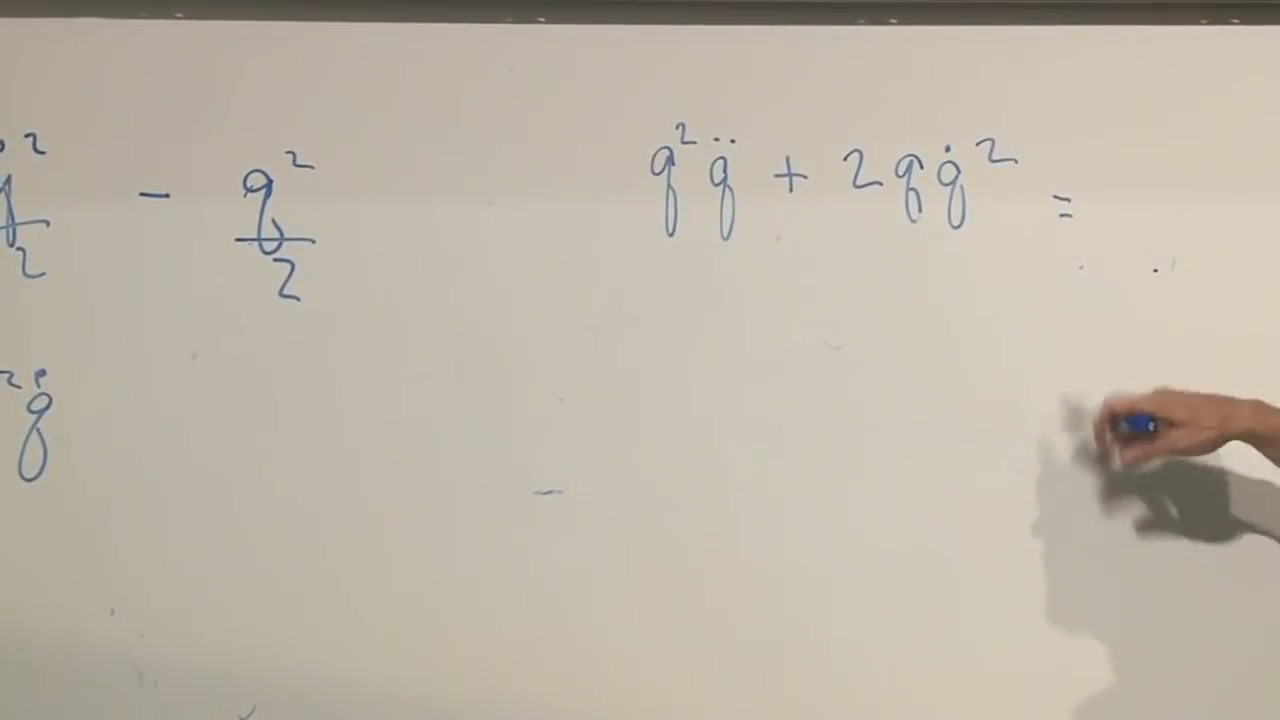
\includegraphics[width=0.80\textwidth]{lecture_05_figure_06.png}
  \caption{Die abgeleitete Impulsgröße im Beispiel mit koordinatenabhängigem kinetischem Term.}
  \lectureframe{01:52:32}
\end{figure}

\begin{classroomqa}
  \audiencequestion{Kann man die Gleichung durch \(q\) teilen?
  \lecturetimestamp{01:53:22--01:53:39}}
  \lecturerresponse{Nur dort, wo \(q\neq0\) gilt. Bei \(q=0\) sind der Koeffizient des kinetischen Terms und die Legendre-Abbildung entartet; durch Division würde man daher einen singulären Punkt ausschließen, der gesondert behandelt werden muss.}
\end{classroomqa}

Die Hamiltonfunktion lautet
\begin{align}
  H&=p\dot q-L
  \notag\\
   &=q^2\dot q^2-
     \left(\frac12q^2\dot q^2-\frac12q^2\right)
  \notag\\
   &=\frac12q^2\dot q^2+\frac12q^2.
  \label{eq:l5-nonstandard-h}
\end{align}

\begin{classroomqa}
  \audiencequestion{Kann \(q^2\dot q^2/2\) weiterhin als kinetische Energie bezeichnet werden?
  \lecturetimestamp{01:54:41--01:55:07}}
  \lecturerresponse{Ja. In diesem ausgearbeiteten Beispiel hat die Hamiltonfunktion wieder die Form eines positiven kinetischen Terms plus eines Potenzialterms. Entscheidend ist, dass die formalen Definitionen auch ohne vorherige Annahme der elementaren Form mit konstanter Masse funktionieren.}
\end{classroomqa}

\section{Dissipation und der tiefere Ursprung des Formalismus}

\begin{classroomqa}
  \audiencequestion{Wie wird Reibung in eine Lagrangefunktion aufgenommen?
  \lecturetimestamp{01:55:09--01:56:17}}
  \lecturerresponse{In dem hier betrachteten einfachen, abgeschlossenen System mit endlich vielen Freiheitsgraden nicht als fundamentale Kraft. Makroskopische Reibung ist ein statistischer Effekt, der aus einer enormen Zahl mikroskopischer Freiheitsgrade hervorgeht. Die Atome gehorchen weiterhin der zugrunde liegenden Mechanik, doch eine reduzierte Beschreibung, die sie nicht verfolgt, zeigt Dissipation.}
\end{classroomqa}

\begin{classroomqa}
  \audiencequestion{Wie gelangte Hamilton zu seiner Formulierung?
  \lecturetimestamp{01:56:22--01:56:37}}
  \lecturerresponse{Hier wurde keine historische Herleitung gegeben. Für den vorliegenden Kurs ist vor allem wichtig zu verstehen, wie die Formulierung funktioniert.}
\end{classroomqa}

\begin{classroomqa}
  \audiencequestion{Gibt es ein allgemeineres Verfahren, um eine Lagrangefunktion zu finden, wenn sie nicht offensichtlich die Form \(T-V\) hat?
  \lecturetimestamp{01:56:43--01:58:54}}
  \lecturerresponse{Experimente, eine begründete Vermutung, ein Symmetrieprinzip oder die Rekonstruktion aus gewünschten Gleichungen können die Funktion liefern. Die Analysis selbst zu fragen, woher ihre Eingabe kommt, ist so, als fragte man die Definition einer Ableitung, woher \(f(x)\) stammt. Die Analysis sagt uns, was zu tun ist, sobald die Funktion festgelegt ist. Warum die abgeschlossenen Systeme der Natur dieser abstrakten Struktur entsprechen, beantwortet die Quantenmechanik auf einer tieferen Ebene.}
\end{classroomqa}

Dieser Punkt knüpft an die einleitenden Themen des Kurses an. Die fundamentale Hamiltonsche Zeitentwicklung ist deterministisch und umkehrbar, insofern sich Trajektorien nicht vereinigen und Information nicht einfach vernichtet wird. Der Zusammenhang zwischen dieser Eigenschaft und der Phasenraumformulierung wird schrittweise entwickelt.

\begin{classroomqa}
  \audiencequestion{Ist die Variationsrechnung lediglich rückwärts von den gewünschten klassischen Gleichungen ausgegangen, und erhält die Quantenmechanik ihre Lagrangefunktion auf dieselbe Weise?
  \lecturetimestamp{01:59:37--02:01:07}}
  \lecturerresponse{Bei der elementaren klassischen Konstruktion kann man tatsächlich eine Wirkung wählen, deren stationäre Wege die bekannten Gleichungen ergeben. In der Quantenmechanik ist die logische Reihenfolge eine andere: Sie geht auf natürliche Weise von der Hamiltonfunktion aus und kann zu einer Lagrangebeschreibung gelangen. Dort ist die Hamiltonfunktion anschaulicher, obwohl sie in der klassischen Mechanik zunächst abstrakt erscheint.}
\end{classroomqa}

\begin{classroomqa}
  \audiencequestion{Kann die Quantenmechanik Reibung beschreiben?
  \lecturetimestamp{02:01:08--02:02:05}}
  \lecturerresponse{Ja, aber eine fundamentale Beschreibung muss die Freiheitsgrade der Umgebung einschließen. Ein Teilchen, das sich durch eine viskose Flüssigkeit bewegt, lässt sich nicht vollständig beschreiben, ohne auch die Teilchen der Flüssigkeit einzubeziehen. Reibung ist der komplizierte kollektive Effekt, der entsteht, wenn diese Freiheitsgrade nicht einzeln verfolgt werden.}
\end{classroomqa}

\chapter{Beschränkte Systeme und Hamiltonsche Bewegung}

\lectureoverview{Zwei beschränkte Systeme zeigen, weshalb die Lagrangesche Mechanik so wirksam ist: Sobald geeignete Koordinaten gewählt sind, ergeben sich die Bewegungsgleichungen und ihre Erhaltungssätze ohne eine explizite Berechnung der Zwangskräfte. Dieselben Beispiele führen anschließend zur Hamiltonschen Mechanik, in der Koordinaten und Impulse den Phasenraum bilden, der harmonische Oszillator zu einer starren Rotation wird und Hamiltons zwei Gleichungen erster Ordnung jeweils eine Euler--Lagrange-Gleichung zweiter Ordnung ersetzen.}

\section{Was es bedeutet, ein mechanisches Problem zu lösen}

Der unmittelbare Zweck der Lagrange-Methode ist praktischer Natur. Ein auf einem Boden gleitender Keil und ein Doppelpendel lassen sich beide mit den Newtonschen Gesetzen behandeln, doch die unbekannten Kontaktkräfte und Spannungen machen die Rechnung schnell mühsam. Kennt man die Regeln der Lagrangeschen Mechanik, werden dieselben Probleme zu einer Folge überschaubarer Schritte:
\begin{enumerate}
  \item unabhängige Koordinaten wählen, die eine momentane Konfiguration beschreiben;
  \item kinetische und potenzielle Energie in diesen Koordinaten ausdrücken;
  \item \(L=T-V\) aufstellen und die Euler--Lagrange-Gleichungen anwenden.
\end{enumerate}

Für den gegenwärtigen Zweck gilt ein Problem bereits als \emph{gelöst}, wenn seine Bewegungsgleichungen korrekt aufgestellt sind. Vielleicht möchte man noch eine geschlossene Lösung für die Bahnkurve finden, doch das ist eine separate Frage. Nichtlineare Differentialgleichungen lassen sich numerisch integrieren, sobald das mechanische Problem vollständig aufgestellt ist. Die Schwierigkeit liegt oft nicht in der Integration, sondern darin, Variablen zu finden, die die Zwangsbedingungen einbeziehen, ohne redundante unbekannte Kräfte einzuführen.

\section{Ein Teilchen gleitet auf einem beweglichen Keil}

Betrachten wir einen Keil der Masse \(M\), der ohne Reibung auf einer horizontalen Ebene gleiten kann. Ein Punktteilchen der Masse \(m\) ist darauf beschränkt, auf der schiefen Fläche zu bleiben. Es gibt zwei Freiheitsgrade: Einer gibt die Lage des Keils an, der andere die Lage des Teilchens auf dem Keil.

Seien
\begin{equation}
  \begin{aligned}
    X&=\text{horizontal position of the wedge corner},\\
    x&=\text{horizontal displacement of the particle}\\[-0.2em]
     &\phantom{={}}\text{from that corner}.
  \end{aligned}
  \label{eq:l6-wedge-coordinates}
\end{equation}
Die absolute horizontale Koordinate des Teilchens ist somit \(X+x\). Die Wahl ist nicht eindeutig. Stattdessen könnten wir den Abstand entlang der schiefen Ebene oder die absolute horizontale Koordinate des Teilchens verwenden. Jedes nicht redundante Koordinatenpaar, das dieselben Konfigurationen beschreibt, ist zulässig; manche Paare machen die Struktur jedoch deutlicher als andere.

Bei einem festen Neigungswinkel \(\beta\) ist die vertikale Verschiebung \(y\) keine unabhängige Koordinate:
\begin{equation}
  y=x\tan\beta,
  \qquad
  \dot y=\dot x\tan\beta.
  \label{eq:l6-wedge-constraint}
\end{equation}
Wir betrachten den Spezialfall \(\beta=45^\circ\), sodass \(y=x\) und
\(\dot y=\dot x\). Diese Vereinfachung beseitigt trigonometrische Faktoren, ohne die Aussage des Beispiels zu verändern.

\begin{figure}[htbp]
  \centering
  \includegraphics[width=0.84\textwidth]{lecture_06_figure_06.png}
  \caption{Der bewegliche Keil, das an ihn gebundene Teilchen sowie die horizontalen und vertikalen Geschwindigkeitskomponenten, die im Beispiel mit \(45^\circ\) verwendet werden.}
  \lectureframe{00:10:25}
\end{figure}

Die kinetische Energie des Keils ist
\begin{equation}
  T_{M}=\frac{M}{2}\dot X^2.
  \label{eq:l6-wedge-kinetic}
\end{equation}
Die horizontale Geschwindigkeit des Teilchens beträgt \(\dot X+\dot x\), seine vertikale Geschwindigkeit \(\dot x\). Damit ist seine kinetische Energie
\begin{equation}
  T_m=\frac{m}{2}\left[(\dot X+\dot x)^2+\dot x^2\right].
  \label{eq:l6-particle-kinetic}
\end{equation}
Wählen wir \(x=0\) als Nullniveau der Gravitationsenergie, so gilt \(V=mgx\).
Somit folgt
\begin{equation}
  L=\frac{M}{2}\dot X^2
    +\frac{m}{2}\left[(\dot X+\dot x)^2+\dot x^2\right]
    -mgx.
  \label{eq:l6-wedge-lagrangian}
\end{equation}

\begin{figure}[htbp]
  \centering
  \includegraphics[width=0.86\textwidth]{lecture_06_figure_07.png}
  \caption{Die Keilgeometrie, \(V=mgx\) und die beiden Beiträge zur kinetischen Energie, an der Tafel zusammengestellt.}
  \lectureframe{00:14:15}
\end{figure}

\subsection{Der kanonische Impuls ist durch die Lagrange-Funktion definiert}

Die kanonischen Impulse werden durch die Lagrange-Funktion definiert und nicht anhand der Geschwindigkeit eines einzelnen Teilchens erraten:
\begin{align}
  p_X&=\frac{\partial L}{\partial\dot X}
      =M\dot X+m(\dot X+\dot x),
      \label{eq:l6-wedge-pX}\\
  p_x&=\frac{\partial L}{\partial\dot x}
      =m(\dot X+\dot x)+m\dot x.
      \label{eq:l6-wedge-px}
\end{align}
Der erste Ausdruck ist der gewöhnliche horizontale Gesamtimpuls: Der Keil trägt \(M\dot X\) bei, das Teilchen \(m(\dot X+\dot x)\). Hier tritt er als der zur Koordinate \(X\) konjugierte Impuls auf.

\begin{figure}[htbp]
  \centering
  \includegraphics[width=0.86\textwidth]{lecture_06_figure_08.png}
  \caption{Die zu der Keilkoordinate \(X\) und der Relativkoordinate des Teilchens \(x\) konjugierten kanonischen Impulse.}
  \lectureframe{00:18:05}
\end{figure}

Die Lagrange-Funktion hängt nicht explizit von \(X\) ab. Eine horizontale Verschiebung des gesamten Systems bewirkt die Transformation
\begin{equation}
  \delta X=\epsilon,
  \qquad
  \delta x=0.
  \label{eq:l6-wedge-translation}
\end{equation}
Die allgemeine Regel für infinitesimale Symmetrien
\begin{equation}
  \delta q_i=\epsilon f_i(q),
  \qquad
  Q=\sum_i p_i f_i
  \label{eq:l6-noether-rule}
\end{equation}
liefert daher \(Q=p_X\). Gleichbedeutend damit ist, dass \(X\) zyklisch ist und
\begin{equation}
  \dot p_X=\frac{\partial L}{\partial X}=0.
  \label{eq:l6-wedge-conservation}
\end{equation}

Eine entsprechende Symmetrie unter vertikalen Verschiebungen gibt es nicht. Der Keil darf sich nicht vertikal bewegen, und eine Änderung der Höhe des Teilchens verändert die Gravitationsenergie. Der horizontale Impuls ist erhalten; der vertikale Impuls dieses beschränkten Teilsystems ist es nicht.

Für die Relativkoordinate lautet die Euler--Lagrange-Gleichung
\begin{equation}
  \dot p_x=\frac{\partial L}{\partial x}=-mg.
  \label{eq:l6-wedge-force}
\end{equation}
An dieser Stelle musste an der Tafel ein Vorzeichen korrigiert werden. Verlässlich ist es, von \(L=T-V\) auszugehen: Da \(V=mgx\), ist die Ableitung der Lagrange-Funktion \(-mg\). Dass \(x\) als horizontale Verschiebung eingeführt wurde, hebt die Wirkung der Schwerkraft in ihrer Gleichung nicht auf, denn die Zwangsbedingung verknüpft diese horizontale Verschiebung mit der vertikalen Höhe \(y=x\).

Es ist weder eine Normalkraft noch eine Reaktionskraft aufgetreten. Diese Kräfte nehmen genau die Werte an, die zur Aufrechterhaltung der Zwangsbedingungen erforderlich sind. Bei der Newton-Methode würde man sie einführen und zusammen mit den Beschleunigungen bestimmen; durch die verallgemeinerten Koordinaten werden sie überflüssig.

\section{Das Doppelpendel und die Kunst der Koordinatenwahl}

Nun hängen wir zwei Massen von je einer Einheit an zwei masselose Stäbe der Länge eins. Der erste Stab bildet mit der nach unten gerichteten Vertikalen den Winkel \(\theta\). Für den zweiten Freiheitsgrad haben wir die Wahl: Wir können den zweiten absoluten Winkel \(\phi\) oder den Relativwinkel \(\alpha\) zwischen den Stäben verwenden.

Der Relativwinkel macht die Struktur deutlicher. Schalten wir die Schwerkraft vorübergehend aus. Eine starre Rotation des gesamten Systems ändert seine absolute Orientierung, nicht aber den Winkel zwischen den Stäben:
\begin{equation}
  \theta\longrightarrow\theta+\epsilon,
  \qquad
  \alpha\longrightarrow\alpha.
  \label{eq:l6-double-rotation}
\end{equation}
Bei dieser Wahl wirkt die Rotationssymmetrie nur auf eine Koordinate. Andere Koordinatensysteme sind deshalb nicht falsch. Mit dieser Wahl sind die Symmetrie und damit auch die Erhaltungsgröße leichter zu erkennen.

\begin{figure}[htbp]
  \centering
  \includegraphics[width=0.76\textwidth]{lecture_06_figure_09.png}
  \caption{Das Doppelpendel mit \(\theta\) als erstem Absolutwinkel und \(\alpha\) als Winkel des zweiten Stabs relativ zum ersten.}
  \lectureframe{00:29:20}
\end{figure}

Um die kinetische Energie zu bestimmen, verwenden wir vorübergehend kartesische Koordinaten als Hilfsgrößen für die Rechnung. Bei einer nach unten positiven vertikalen Koordinate befindet sich die erste Pendelmasse bei
\begin{equation}
  x_1=\sin\theta,
  \qquad
  y_1=\cos\theta,
  \label{eq:l6-bob-one-position}
\end{equation}
und damit gilt
\begin{equation}
  \dot x_1=\dot\theta\cos\theta,
  \qquad
  \dot y_1=-\dot\theta\sin\theta,
  \qquad
  \dot x_1^2+\dot y_1^2=\dot\theta^2.
  \label{eq:l6-bob-one-velocity}
\end{equation}
Die zweite Pendelmasse befindet sich bei
\begin{align}
  x_2&=\sin\theta+\sin(\theta+\alpha),\\
  y_2&=\cos\theta+\cos(\theta+\alpha),
  \label{eq:l6-bob-two-position}
\end{align}
und beispielsweise gilt
\begin{equation}
  \dot x_2=\dot\theta\cos\theta
  +(\dot\theta+\dot\alpha)\cos(\theta+\alpha),
  \label{eq:l6-bob-two-xvelocity}
\end{equation}
mit einem entsprechenden Ausdruck für \(\dot y_2\).

\begin{figure}[htbp]
  \centering
  \includegraphics[width=0.88\textwidth]{lecture_06_figure_10.png}
  \caption{Hilfsweise eingeführte kartesische Koordinaten für die beiden Pendelmassen. Sie dienen zur Berechnung der Geschwindigkeiten und werden nicht als zusätzliche Freiheitsgrade eingeführt.}
  \lectureframe{00:35:25}
\end{figure}

Die Summe der beiden kinetischen Energien ergibt den konsistenten Ausdruck unten. Der gemischte Term folgt aus
\begin{equation*}
  \cos A\cos B+\sin A\sin B=\cos(A-B).
\end{equation*}
\begin{equation}
  T=\dot\theta^2
    +\frac12(\dot\theta+\dot\alpha)^2
    +\dot\theta(\dot\theta+\dot\alpha)\cos\alpha.
  \label{eq:l6-double-kinetic}
\end{equation}

\begin{classroomqa}
  \audiencequestion{Enthält dieser Ausdruck bereits die kinetische Energie beider Pendelmassen, oder ist ein Faktor ein halb verloren gegangen?
  \lecturetimestamp{00:38:06--00:38:27}}
  \lecturerresponse{Er enthält beide Beiträge. Er ergibt sich aus
  \(\tfrac12(\dot x_1^2+\dot y_1^2+\dot x_2^2+\dot y_2^2)\).
  Zwei gleiche Beiträge ergeben zusammen den ersten Term
  \(\dot\theta^2\); ein Faktor fehlt nicht.}
\end{classroomqa}

Ohne Schwerkraft hängt \(L=T\) nicht explizit von \(\theta\) ab. Daher gilt
\begin{equation}
  \dot p_\theta=\frac{\partial L}{\partial\theta}=0,
  \label{eq:l6-double-angular-conservation}
\end{equation}
und \(p_\theta\) ist der gesamte Drehimpuls. Beachten wir die genaue Bedeutung der Aussage, dass \(\theta\) nicht auftritt: \(\dot\theta\) tritt durchaus auf, die nicht abgeleitete Koordinate jedoch nicht.

Mit der Wiedereinschaltung der Schwerkraft wird die globale Rotationssymmetrie gebrochen. Bei der oben verwendeten Konvention mit nach unten positiver Vertikalrichtung ergibt eine zweckmäßige Wahl des Nullniveaus
\begin{equation}
  V=-g(y_1+y_2)
   =-g\left[2\cos\theta+\cos(\theta+\alpha)\right].
  \label{eq:l6-double-potential}
\end{equation}
Eine additive Konstante änderte daran nichts. Entscheidend ist, dass \(\theta\) nun explizit auftritt, sodass der zugehörige konjugierte Impuls nicht mehr erhalten ist. Die Energie bleibt erhalten, weil die Lagrange-Funktion nicht explizit von der Zeit abhängt.

\begin{classroomqa}
  \audiencequestion{Sollte an der Tafel stehen:
  \(\dot\theta-\dot\alpha\) oder
  \(\dot\theta+\dot\alpha\)?
  \lecturetimestamp{00:43:00--00:43:54}}
  \lecturerresponse{Bei der hier verwendeten Orientierung ist das Pluszeichen erforderlich. Es entspricht der Konvention in Gl.~\eqref{eq:l6-bob-two-position} und wird in der kinetischen Energie in Gl.~\eqref{eq:l6-double-kinetic} beibehalten. Eine Umkehr der Definition des positiven \(\alpha\) ändert die entsprechenden Vorzeichen; dann müssen jedoch alle Vorkommen konsistent angepasst werden. An der Tafel wurden die beiden Konventionen vermischt.}
\end{classroomqa}

\begin{figure}[htbp]
  \centering
  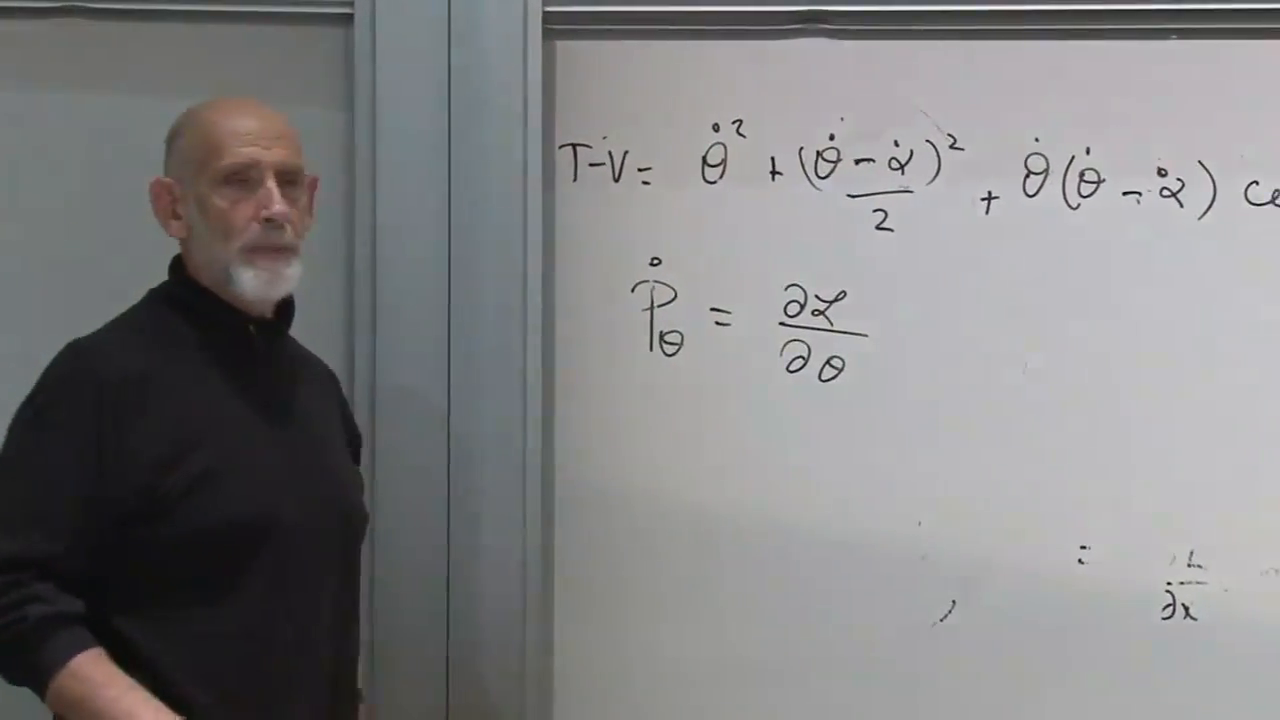
\includegraphics[width=0.84\textwidth]{lecture_06_figure_02.png}
  \caption{Die Pendelrechnung ohne Schwerkraft und \(\dot p_\theta=\partial L/\partial\theta\). Die obere Zeile an der Tafel behält die im Fragebeitrag erörterte, vor Ort vorzeicheninkonsistente Notation bei; die vereinheitlichte Formel steht in Gl.~\eqref{eq:l6-double-kinetic}.}
  \lectureframe{00:45:50}
\end{figure}

Sobald \(T\) und \(V\) bekannt sind, ergeben sich die übrigen Gleichungen durch Ableitung. Auch die Stabspannungen und die Kräfte, die die festen Längen gewährleisten, sind durch die Koordinatenwahl entfallen.

\subsection{Was Erhaltung aussagt und was nicht}

\begin{classroomqa}
  \audiencequestion{Kann man den Gleichungen unmittelbar entnehmen, ob das Doppelpendel chaotisch ist?
  \lecturetimestamp{00:44:57--00:45:25}}
  \lecturerresponse{Meistens lässt sich das nicht durch einfache Betrachtung erkennen. Wenn sich Parameter oder Energien ändern, kann ein System von regelmäßigem zu chaotischem Verhalten übergehen. Um dieses Gebiet zu behandeln, braucht man mehr Struktur als den bloßen Anblick der Gleichungen; es wird später wieder aufgegriffen.}
\end{classroomqa}

\begin{classroomqa}
  \audiencequestion{Ist in einem konservativen System jedes \(\dot p_i\) gleich null?
  \lecturetimestamp{00:45:25--00:46:24}}
  \lecturerresponse{Nein. Die allgemeine Gleichung lautet
  \(\dot p_i=\partial L/\partial q_i\). Sie verschwindet nur, wenn \(q_i\) zyklisch ist. Eine zyklische Koordinate ist der besonders einfache Fall, in dem eine Symmetrie so dargestellt wird, dass sie eine Koordinate verschiebt und die übrigen unverändert lässt.}
\end{classroomqa}

Wenn es allein um die numerische zeitliche Entwicklung geht, funktioniert auch ein unpraktisches Koordinatensystem; es führt lediglich zu längeren Gleichungen. Der Gewinn einer geschickten Wahl ist konzeptioneller Art: Der erhaltene Impuls ist bereits sichtbar, bevor die Gleichungen gelöst werden.

\begin{classroomqa}
  \audiencequestion{Bewegt sich ein Doppelpendel ohne Schwerkraft so einfach wie ein einzelnes freies Pendel?
  \lecturetimestamp{00:47:02--00:47:35}}
  \lecturerresponse{Ein einzelner freier Rotor dreht sich gleichförmig, weil sein einziger Drehimpuls seine Bewegung festlegt. Ein Doppelpendel kann eine sehr komplizierte Relativbewegung ausführen und dabei dennoch den Gesamtdrehimpuls erhalten. Sind anfangs beide Winkelgeschwindigkeiten null, bleibt es in Ruhe; andernfalls wechselwirken die beiden Teile.}
\end{classroomqa}

\begin{classroomqa}
  \audiencequestion{Sind \(\dot\theta\) und \(\dot\alpha\) einzeln konstant, wenn die Schwerkraft fehlt?
  \lecturetimestamp{00:47:36--00:52:42}}
  \lecturerresponse{Nein. Erhaltung bedeutet \(\dot p_\theta=0\), nicht \(\ddot\theta=0\) oder \(\ddot\alpha=0\). Der Ausdruck für \(p_\theta=\partial L/\partial\dot\theta\) enthält beide Winkelgeschwindigkeiten und hängt von \(\alpha\) ab. Die Stäbe übertragen Drehmomente, sodass die beiden Pendelmassen Drehimpuls und Energie austauschen können. Das ist vergleichbar mit zwei durch eine Feder verbundenen Massen: Gesamtimpuls und Schwerpunktsgeschwindigkeit bleiben konstant, während die einzelnen Geschwindigkeiten oszillieren. Das rotatorische Analogon ist eine bestimmte kollektive Kombination, nicht einer der beiden Winkel für sich.}
\end{classroomqa}

\begin{classroomqa}
  \audiencequestion{Werden die Kräfte, durch die Drehimpuls ausgetauscht wird, über die Stäbe übertragen?
  \lecturetimestamp{00:52:43--00:53:34}}
  \lecturerresponse{Ja. Eine entlang eines Stabs übertragene Kraft muss nicht durch den Drehpunkt der anderen Bewegungslinie wirken und kann deshalb ein Drehmoment ausüben. Ein Drehmoment ist schlicht die Drehwirkung einer Kraft; hier führt es zu von null verschiedenen Winkelbeschleunigungen der einzelnen Pendel.}
\end{classroomqa}

\section{Der Hamiltonian als dritte Formulierung}

Der Hamiltonian ist die Energie, doch das ist nur seine erste Bedeutung. Er bildet auch die Grundlage einer dritten Formulierung der Mechanik. Die Newtonschen Gleichungen verwenden Kräfte und Beschleunigungen. Das Prinzip der stationären Wirkung führt zu den Euler--Lagrange-Gleichungen. Für reguläre Systeme ist die Hamiltonsche Mechanik dazu äquivalent, doch ihre Variablen und ihre Geometrie sehen anders aus.

Statt \(q_i\) und \(\dot q_i\) verwenden wir \(q_i\) und die zugehörigen konjugierten Impulse \(p_i\). Zur Beschreibung des Zustands eines Systems mit \(n\) Freiheitsgraden sind in beiden Darstellungen \(2n\) Zahlen erforderlich: entweder Orte und Geschwindigkeiten oder Orte und Impulse. Die Verbindung zwischen ihnen lautet
\begin{equation}
  p_i=\frac{\partial L}{\partial\dot q_i}.
  \label{eq:l6-legendre-map}
\end{equation}
Wenn sich diese Beziehungen nach den Geschwindigkeiten \(\dot q_i(q,p)\) auflösen lassen, definieren wir
\begin{equation}
  H(q,p)=\sum_i p_i\dot q_i-L(q,\dot q).
  \label{eq:l6-hamiltonian-definition}
\end{equation}
Die Geschwindigkeiten auf der rechten Seite werden dann durch \(q\) und \(p\) ersetzt. Diese Umkehrbarkeit ist die Voraussetzung einer regulären Legendre-Transformation. Bei singulären Lagrange-Funktionen ist eine allgemeinere Theorie der Zwangsbedingungen erforderlich; sie wird von dieser elementaren Konstruktion nicht erfasst.

\subsection{Umkehrbarkeit vor der Differentialrechnung}

Betrachten wir eine endliche Menge abstrakter Zustände, die durch Pfeile verbunden sind. Auch eine deterministische Regel kann unumkehrbar sein, wenn zwei frühere Zustände in einen späteren übergehen. Die Zukunft ist eindeutig, die Vergangenheit jedoch nicht. Kehrt man alle Pfeile um, erhält man den entgegengesetzten Fehler: Ein Zustand verzweigt sich in mehrere mögliche Zukünfte. Im ersten Bild laufen die Pfeile zusammen, im zweiten auseinander.

\begin{figure}[htbp]
  \centering
  \includegraphics[width=0.86\textwidth]{lecture_06_figure_11.png}
  \caption{Abbildungen abstrakter Zustände, die umkehrbare Zyklen mit unzulässigem Zusammenlaufen und Auseinanderlaufen vergleichen.}
  \lectureframe{00:56:20}
\end{figure}

Der Hamiltonsche Fluss liefert eine kontinuierliche Entsprechung dieser Aussage. Eine Wolke von Phasenraumpunkten kann sich bewegen und verformen, aber es kann weder eine Senke entstehen, die Unterschiede zwischen Zuständen auslöscht, noch eine Quelle, die aus einem Zustand mehrere Zukünfte hervorbringt. Der Beweis folgt später; vorerst veranschaulichen die Diagramme die Geometrie.

\begin{classroomqa}
  \audiencequestion{Ist das Diagramm der abstrakten Zustände als ein Objekt zu verstehen, das sich in einem Gravitationsfeld bewegt?
  \lecturetimestamp{00:58:02--00:58:35}}
  \lecturerresponse{Nein. Die Punkte stellen lediglich abstrakte Zustände dar, und die Pfeile geben eine Regel für Zustandsänderungen an. Der Zeichnung wurde keine räumliche oder gravitative Bedeutung zugewiesen.}
\end{classroomqa}

\begin{classroomqa}
  \audiencequestion{Wodurch unterscheidet sich eine unzulässige zusammenlaufende Zustandsabbildung von einem Schwarzen Loch?
  \lecturetimestamp{00:58:40--00:59:28}}
  \lecturerresponse{Nur mit Mühe und unter Berücksichtigung feiner Einzelheiten. Die Frage ist berechtigt, doch eine korrekte Antwort erfordert eine sorgfältige Beschreibung des vollständigen Zustands und seiner quantengravitativen Entwicklung. Das elementare Diagramm reicht für eine Entscheidung nicht aus.}
\end{classroomqa}

\section{Ein an den Phasenraum angepasster Oszillator}

Bevor wir die allgemeinen Gleichungen herleiten, betrachten wir einen harmonischen Oszillator in bewusst angepassten Variablen:
\begin{equation}
  L=\frac{1}{2\omega}\dot q^2-\frac{\omega}{2}q^2.
  \label{eq:l6-rescaled-lagrangian}
\end{equation}
Sein konjugierter Impuls ist
\begin{equation}
  p=\frac{\partial L}{\partial\dot q}=\frac{\dot q}{\omega},
  \qquad
  \dot q=\omega p.
  \label{eq:l6-rescaled-momentum}
\end{equation}
Einsetzen in Gl.~\eqref{eq:l6-hamiltonian-definition} ergibt
\begin{align}
  H&=p\dot q-L\\
   &=\omega p^2-\frac{\omega p^2}{2}+\frac{\omega q^2}{2}
    =\frac{\omega}{2}(p^2+q^2).
  \label{eq:l6-oscillator-hamiltonian}
\end{align}

\begin{figure}[htbp]
  \centering
  \includegraphics[width=0.86\textwidth]{lecture_06_figure_12.png}
  \caption{Die Legendre-Transformation des angepassten Oszillators und der symmetrische Hamiltonian \(H=\tfrac{\omega}{2}(p^2+q^2)\).}
  \lectureframe{01:08:20}
\end{figure}

Der Raum der \(q\) und \(p\) ist der Phasenraum. Bei einem Freiheitsgrad ist er eine zweidimensionale Ebene; bei zwei Freiheitsgraden ein vierdimensionaler Phasenraum. Bei fester Oszillatorenergie gilt
\begin{equation}
  p^2+q^2=\frac{2H}{\omega},
  \label{eq:l6-energy-circle}
\end{equation}
sodass die Bahn auf einem Kreis bleibt. Die Energieerhaltung beschränkt die Bewegung auf eine solche Kurve.

\begin{figure}[htbp]
  \centering
  \includegraphics[width=0.82\textwidth]{lecture_06_figure_13.png}
  \caption{Konzentrische Kreise konstanter Energie in der Oszillator-Phasenebene, mit \(q\) auf der Horizontalen und \(p\) auf der Vertikalen.}
  \lectureframe{01:13:20}
\end{figure}

\section{Herleitung der Hamilton-Gleichungen}

Die Herleitung beruht auf dem Differential einer Funktion mehrerer Variablen. Für \(F(q,p)\) gilt:
\begin{equation}
  \delta F=\sum_i\left(
  \frac{\partial F}{\partial q_i}\delta q_i
  +\frac{\partial F}{\partial p_i}\delta p_i\right).
  \label{eq:l6-total-differential}
\end{equation}
Die Koeffizienten lassen sich in beide Richtungen ablesen: Der Koeffizient von \(\delta q_i\) ist \(\partial F/\partial q_i\), und der Koeffizient von \(\delta p_i\) ist \(\partial F/\partial p_i\).

Variieren wir nun den definierenden Ausdruck für \(H\):
\begin{align}
  \delta H
  &=\sum_i\left(\dot q_i\,\delta p_i
       +p_i\,\delta\dot q_i\right)-\delta L\\
  &=\sum_i\left(\dot q_i\,\delta p_i
       +p_i\,\delta\dot q_i
       -\frac{\partial L}{\partial q_i}\delta q_i
       -\frac{\partial L}{\partial\dot q_i}\delta\dot q_i\right).
  \label{eq:l6-vary-hamiltonian}
\end{align}
Da \(\partial L/\partial\dot q_i=p_i\), heben sich die beiden Terme \(\delta\dot q_i\) auf. Die Euler--Lagrange-Gleichungen liefern \(\partial L/\partial q_i=\dot p_i\); damit bleibt
\begin{equation}
  \delta H=\sum_i\left(\dot q_i\,\delta p_i
                     -\dot p_i\,\delta q_i\right).
  \label{eq:l6-reduced-variation}
\end{equation}

\begin{figure}[htbp]
  \centering
  \includegraphics[width=0.86\textwidth]{lecture_06_figure_14.png}
  \caption{Die Ausmultiplizierung der Produktregel für \(\delta H\), bevor sich die Terme \(p_i\,\delta\dot q_i\) aufheben.}
  \lectureframe{01:18:40}
\end{figure}

Vergleichen wir Gl.~\eqref{eq:l6-reduced-variation} mit dem allgemeinen Differential in Gl.~\eqref{eq:l6-total-differential}, so ergeben die unabhängigen Koeffizienten Hamiltons Gleichungen:
\begin{equation}
  \boxed{
  \dot q_i=\frac{\partial H}{\partial p_i},
  \qquad
  \dot p_i=-\frac{\partial H}{\partial q_i}.}
  \label{eq:l6-hamilton-equations}
\end{equation}

\begin{figure}[htbp]
  \centering
  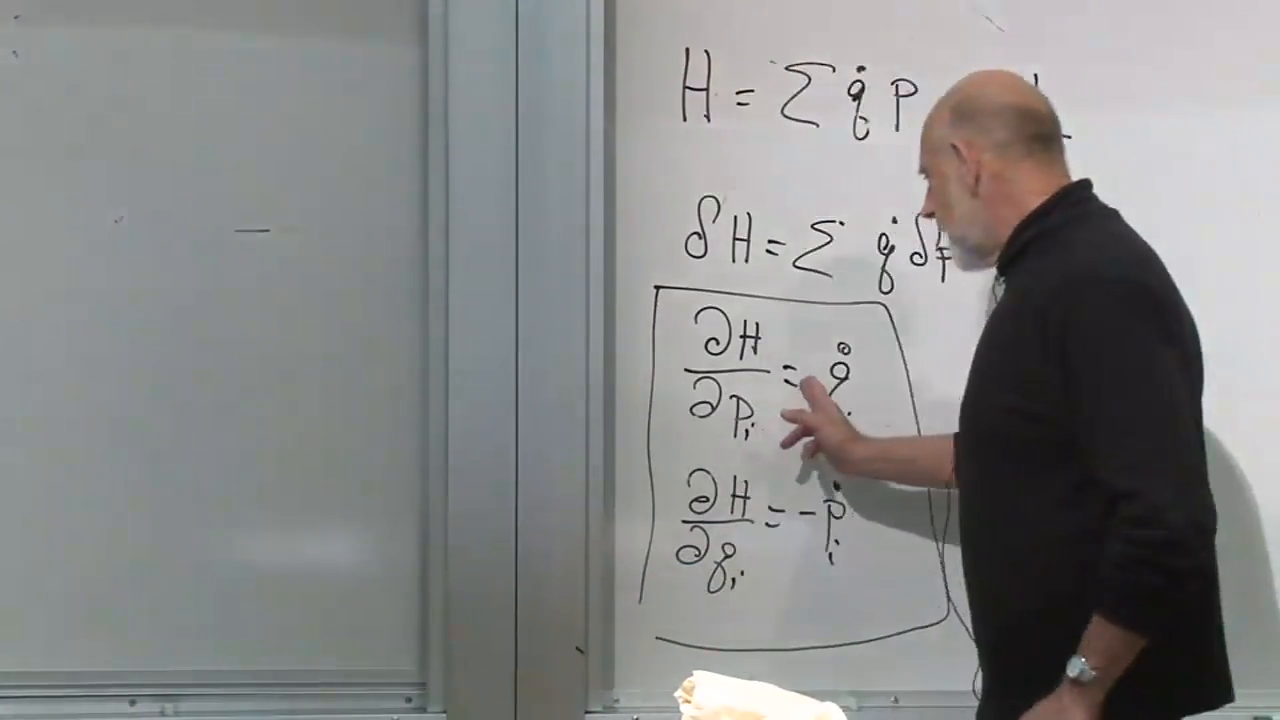
\includegraphics[width=0.78\textwidth]{lecture_06_figure_03.png}
  \caption{Die Definition des Hamiltonians, seine Variation und die eingerahmten kanonischen Gleichungen.}
  \lectureframe{01:22:18}
\end{figure}

Für \(n\) Koordinaten sind dies \(2n\) Gleichungen erster Ordnung. Die Euler--Lagrange-Formulierung liefert dagegen \(n\) Gleichungen zweiter Ordnung. Umfang der Anfangsdaten und physikalischer Gehalt sind identisch.

\section{Die Oszillatorbewegung als starre Rotation}

Wenden wir Gl.~\eqref{eq:l6-hamilton-equations} auf Gl.~\eqref{eq:l6-oscillator-hamiltonian} an, so ergibt sich
\begin{equation}
  \dot q=\omega p,
  \qquad
  \dot p=-\omega q.
  \label{eq:l6-oscillator-first-order}
\end{equation}
Differenzieren wir die erste Gleichung und verwenden die zweite, folgt
\begin{equation}
  \ddot q=\omega\dot p=-\omega^2q.
  \label{eq:l6-oscillator-second-order}
\end{equation}
Die beiden Gleichungen erster Ordnung ergeben also genau die gewöhnliche Oszillatorgleichung zweiter Ordnung, zusammen mit der Definition des Impulses.

Im Phasenraum ist der Geschwindigkeitsvektor am Punkt \((q,p)\) gleich \((\dot q,\dot p)=(\omega p,-\omega q)\) und damit tangential zum Energiekreis. Jeder Radius rotiert mit derselben Winkelgeschwindigkeit \(\omega\). Man kann sich die gesamte Ebene als starres Windrad oder als inkompressible fiktive Flüssigkeit vorstellen. Ihre Punkte kreisen, ohne sich in eine Senke zusammenzudrängen oder von einer Quelle auseinanderzutreiben.

\begin{figure}[htbp]
  \centering
  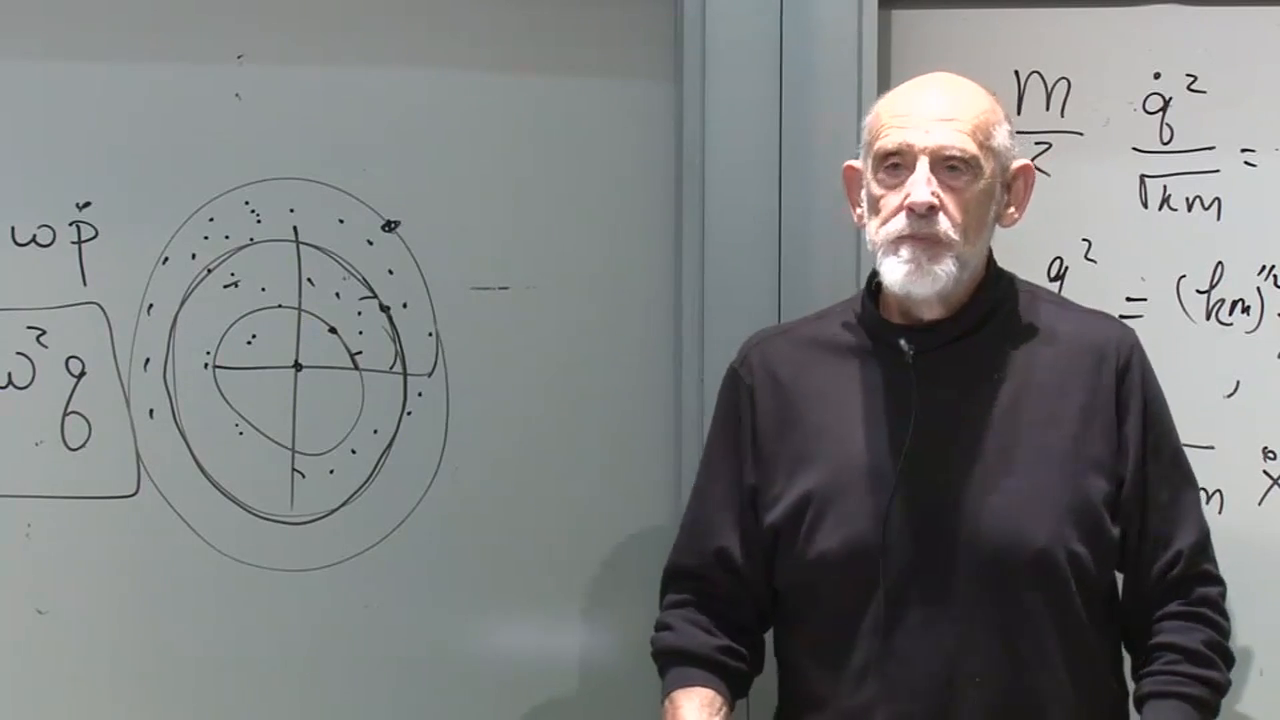
\includegraphics[width=0.86\textwidth]{lecture_06_figure_04.png}
  \caption{Eine Wolke von Anfangspunkten, verteilt auf konzentrische Phasenraumbahnen. Die Hamiltonsche Entwicklung bewegt die Wolke, statt sie in einen ausgezeichneten Zustand kollabieren zu lassen.}
  \lectureframe{01:39:27}
\end{figure}

\begin{figure}[htbp]
  \centering
  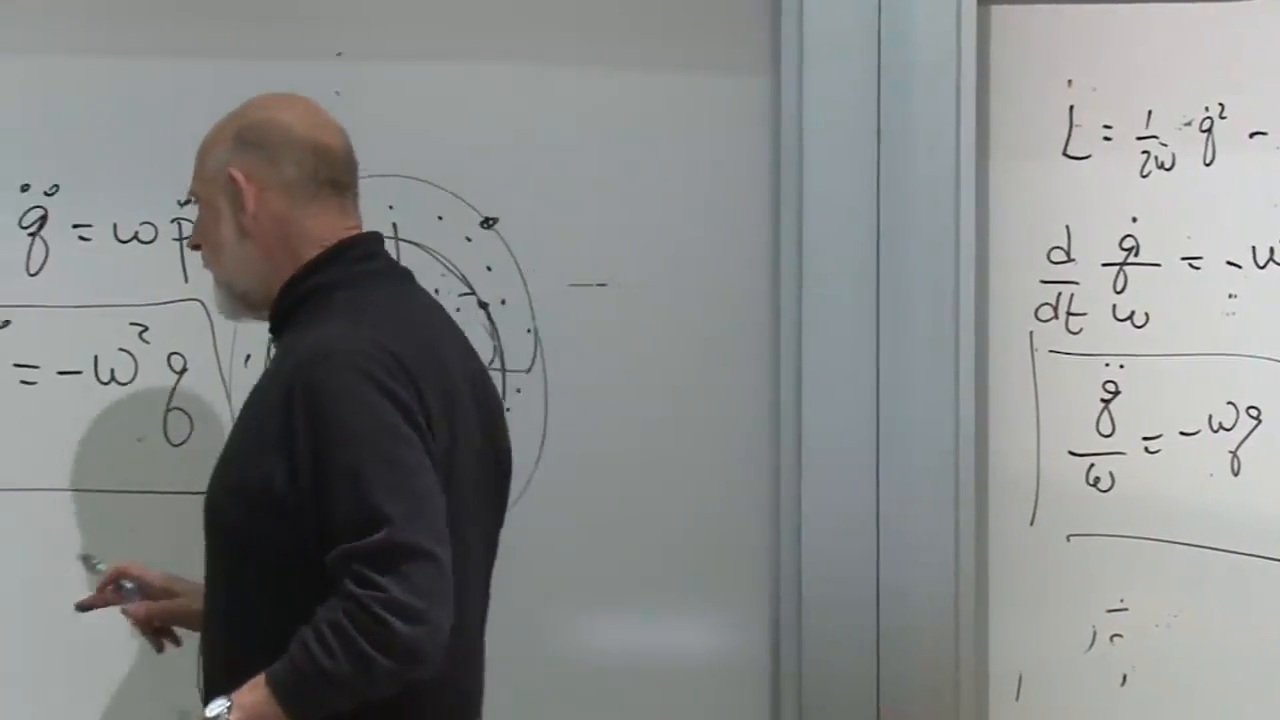
\includegraphics[width=0.90\textwidth]{lecture_06_figure_05.png}
  \caption{Das Phasenportrait des Oszillators neben der äquivalenten Euler--Lagrange-Gleichung
  \(\ddot q/\omega=-\omega q\).}
  \lectureframe{01:42:10}
\end{figure}

Im nächsten Schritt wird die Analogie zur Flüssigkeit zu einem Satz präzisiert: Der Hamiltonsche Fluss weist lokal weder Zusammenlaufen noch Auseinanderlaufen auf. Dieses Ergebnis verknüpft die kontinuierliche Mechanik wieder mit den umkehrbaren Zustandsabbildungen, die zu Beginn des Kurses betrachtet wurden.

\section{Fragen, die die Koordinatenwahl verdeutlichen}

\begin{classroomqa}
  \audiencequestion{Ist die Annahme, dass sich die Geschwindigkeiten durch \(q\) und \(p\) ausdrücken lassen, ein Satz oder eine empirische Eigenschaft physikalischer Systeme?
  \lecturetimestamp{01:29:08--01:29:45}}
  \lecturerresponse{Im Rahmen dieser elementaren Einführung handelt es sich um eine empirische Regelmäßigkeit, für die es eine tiefer gehende Motivation aus der Quantenmechanik gibt. Genauer gesagt muss Gl.~\eqref{eq:l6-legendre-map} eine bezüglich der Geschwindigkeiten nichtsinguläre Jacobi-Matrix haben. Die moderne Mechanik umfasst auch wichtige singuläre Lagrange-Funktionen, insbesondere bei Systemen mit Zwangsbedingungen und Eichsymmetrie; ihre Hamiltonsche Formulierung erfordert jedoch einen zusätzlichen Formalismus für Zwangsbedingungen.}
\end{classroomqa}

Ein Einwand zu den Einheiten erklärt, weshalb der Oszillator in der ungewohnten Form von Gl.~\eqref{eq:l6-rescaled-lagrangian} geschrieben wurde. Beginnen wir stattdessen mit der gewöhnlichen Koordinate \(x\):
\begin{equation}
  L=\frac{m}{2}\dot x^2-\frac{k}{2}x^2,
  \qquad
  \omega=\sqrt{\frac{k}{m}}.
  \label{eq:l6-ordinary-oscillator}
\end{equation}
Wir wählen
\begin{equation}
  q=(km)^{1/4}x.
  \label{eq:l6-oscillator-rescaling}
\end{equation}
Dann gilt \(q^2=\sqrt{km}\,x^2\) und
\(\dot q^2=\sqrt{km}\,\dot x^2\), wodurch Gl.~\eqref{eq:l6-ordinary-oscillator} genau in Gl.~\eqref{eq:l6-rescaled-lagrangian} übergeht. Das neue \(q\) ist eine angepasste verallgemeinerte Koordinate, keine Länge, und sein konjugierter Impuls \(p\) ist nicht der gewöhnliche mechanische Impuls \(p_x=m\dot x\).

\begin{figure}[htbp]
  \centering
  \includegraphics[width=0.86\textwidth]{lecture_06_figure_15.png}
  \caption{Die Skalierung zur Anpassung der Dimensionen: von der gewöhnlichen Oszillatorkoordinate \(x\) zur angepassten Koordinate \(q=(km)^{1/4}x\).}
  \lectureframe{01:36:10}
\end{figure}

\begin{classroomqa}
  \audiencequestion{Wie kann \(\omega p=\dot q\) dimensionskonsistent sein, und weshalb wurden diese Variablen gewählt?
  \lecturetimestamp{01:29:46--01:39:22}}
  \lecturerresponse{Das Symbol \(q\) muss nicht die Dimension einer Länge haben, und sein konjugierter Impuls \(p\) muss nicht die Dimension von \(m\dot x\) haben. Die Skalierung in Gl.~\eqref{eq:l6-oscillator-rescaling} erhält die Dimensionen der Lagrange-Funktion und sorgt dafür, dass \(q\) und \(p\) symmetrisch in \(H\) eingehen. In den ursprünglichen Variablen gilt:
  \[
    H=\frac{p_x^2}{2m}+\frac{kx^2}{2},
  \]
  Die Kurven konstanter Energie sind daher in der \((x,p_x)\)-Ebene Ellipsen. In der angepassten \((q,p)\)-Ebene sind es Kreise. Die Skalierung wurde gewählt, um diese Symmetrie sichtbar zu machen.}
\end{classroomqa}

\begin{classroomqa}
  \audiencequestion{Wie können \(2n\) Hamilton-Gleichungen erster Ordnung äquivalent zu \(n\) Lagrange-Gleichungen zweiter Ordnung sein?
  \lecturetimestamp{01:39:24--01:42:30}}
  \lecturerresponse{Beim Oszillator differenziert man \(\dot q=\omega p\) und setzt \(\dot p=-\omega q\) ein; das Gleichungspaar wird dann zu \(\ddot q=-\omega^2q\). Geht man direkt von der Lagrange-Funktion aus, erhält man
  \[
    \frac{d}{dt}\left(\frac{\dot q}{\omega}\right)
      =-\omega q,
  \]
  also dieselbe Gleichung zweiter Ordnung. Eine der Hamilton-Gleichungen kann als Definition des Impulses über die Geschwindigkeit aufgefasst werden, während die andere dessen zeitliche Entwicklung beschreibt.}
\end{classroomqa}

\section{Warum Phasenraum und potenzielle Energie wichtig sind}

\begin{classroomqa}
  \audiencequestion{Bedeutet die Leistungsfähigkeit des Hamiltonians, dass der Phasenraum eine bessere geometrische Darstellung als der Konfigurationsraum ist?
  \lecturetimestamp{01:42:33--01:44:38}}
  \lecturerresponse{Sie erfüllen unterschiedliche Zwecke. Im Phasenraum lassen sich Zyklen, Flächen konstanter Energie sowie das Ausbleiben von Zusammenlaufen und Auseinanderlaufen besonders deutlich erkennen. Für andere Fragen kann der Konfigurationsraum geeigneter sein. Der tiefere Grund, \(H\) hervorzuheben, liegt darin, dass es in der Quantenmechanik, einem der modernen Gebiete, auf die diese Mechanik hinführt, zu einem zentralen und anschaulicheren Objekt wird.}
\end{classroomqa}

\begin{classroomqa}
  \audiencequestion{Ist die potenzielle Energie als Integral der Kraft aufzufassen?
  \lecturetimestamp{01:44:40--01:45:45}}
  \lecturerresponse{Für konservative Kräfte ist diese Aussage bis auf eine Konstante und bei passender Vorzeichenwahl richtig. Zweckmäßiger ist die umgekehrte Sicht: Man betrachtet das Potenzial als grundlegend und leitet daraus die verallgemeinerte Kraft ab:
  \[
    F_i=-\frac{\partial V}{\partial q_i}.
  \]
  Genau dieser Term tritt in \(\dot p_i=\partial L/\partial q_i\) auf, wenn \(L=T-V\) gilt und die kinetische Energie nicht explizit von \(q_i\) abhängt.}
\end{classroomqa}

\begin{classroomqa}
  \audiencequestion{Welche ungelösten Probleme der modernen Physik soll dieser Weg beleuchten?
  \lecturetimestamp{01:45:46--01:47:47}}
  \lecturerresponse{Der Weg führt zur Quantengravitation und Kosmologie, zur Elementarteilchenphysik einschließlich des Higgs-Sektors und der Neutrinos, zur Relativitätstheorie, Stringtheorie und Quantenfeldtheorie. Die fortbestehende theoretische Aufgabe ist, diese Bestandteile in eine zusammenhängende Struktur einzufügen, insbesondere die Quantenmechanik mit der Gravitation und die Kosmologie mit der Teilchenphysik zu verbinden. Dies beschrieb den Stand der offenen Fragen, wie er sich 2011 darstellte; es war keine Behauptung, ihre Lösung sei bereits bekannt.}
\end{classroomqa}

Die beiden Beispiele mit Zwangsbedingungen und der Oszillator fügen sich nun zu einem Gesamtbild. Verallgemeinerte Koordinaten beseitigen unnötige Kräfte. Symmetrien bestimmen die erhaltenen kanonischen Impulse. Die Legendre-Transformation ersetzt Geschwindigkeiten durch Impulse, und Hamiltons Gleichungen beschreiben die Dynamik als Fluss im Phasenraum. Beim Oszillator ist dieser Fluss eine starre Rotation; bei einem allgemeinen System liefert seine Geometrie die präzise kontinuierliche Bedeutung umkehrbarer Bewegung.
\chapter{Liouvillescher Satz und Hamiltonscher Fluss}

\lectureoverview{Hamiltons Gleichungen leisten mehr, als die Bewegungsgleichungen nur in anderer Form darzustellen. Sie definieren ein Geschwindigkeitsfeld im Phasenraum, dessen Divergenz verschwindet. Diese einfache Aufhebung ist der Satz von Liouville: Die Hamiltonsche Entwicklung erhält das Phasenraumvolumen. Wir nähern uns dem Satz in der Reihenfolge, in der seine Bedeutung sichtbar wird---zunächst die Energieerhaltung, dann die Flächen konstanter Energie, anschließend ein Fluid möglicher Anfangsbedingungen und schließlich der Gegensatz zwischen volumenbewahrendem Fluss und dissipativem Senkenpunkt. Dieselbe Sprache führt auf natürliche Weise zu Poisson-Klammern.}

\section{Warum eine weitere Form der Mechanik?}

Der Satz, den wir herleiten wollen, ist das kontinuierliche klassische Gegenstück zu den umkehrbaren Zustandsdiagrammen, die zu Beginn des Kurses eingeführt wurden. In einem umkehrbaren diskreten Gesetz führt genau ein Pfeil in jeden Zustand hinein und genau einer aus ihm heraus. Die Gegenwart genügt, um sowohl den nächsten als auch den vorherigen Zustand zu bestimmen. Ein fehlerhaftes Gesetz führt viele Zustände in einen Senkenpunkt: Die Zukunft lässt sich möglicherweise bestimmen, die Vergangenheit jedoch nicht mehr rekonstruieren.

Der Satz von Liouville beschreibt, was aus diesem Unterschied wird, wenn die Zustandsmenge ein kontinuierlicher Phasenraum ist. An die Stelle von einem eingehenden und einem ausgehenden Pfeil tritt die Formulierung \emph{ebenso viel hinein wie hinaus fließt}. Bevor sich das jedoch mathematisch fassen lässt, müssen wir den Fluss aus Hamiltons Gleichungen rekonstruieren.

Dabei ergibt sich ein historisches Rätsel. Hamilton, Jacobi, Lagrange und Poisson entwickelten aufwendige und elegante Formen der klassischen Mechanik, ohne die Quantentheorie zu kennen, in der diese Formen später unverzichtbar werden sollten. Newton hatte ein unmittelbares Ziel: die Planetenbewegung. Auch Lagrange und Hamilton befassten sich mit physikalischen Problemen, doch sie verfolgten Analogien und Strukturen, die weit über eine einzelne Bahn hinausgingen. Das Prinzip der stationären Wirkung in der Mechanik ähnelte den Prinzipien der kürzesten Zeit in der Optik; Strahlen- und Teilchenbewegung ließen sich in parallele mathematische Formen bringen. Sie vereinfachten, ordneten um und vereinheitlichten die Gleichungen, weil die Strukturen selbst physikalischen Gehalt zu besitzen schienen.

Heute wissen wir, wie außerordentlich fruchtbar diese Intuition war. Logisch lassen sich viele Merkmale der klassischen Mechanik als Grenzfälle der Quantenmechanik verstehen. Historisch verlief die Entwicklung umgekehrt: Zuerst wurden die klassischen Strukturen gefunden, und erst viel später wurde ihre tiefere Bedeutung klar. Ein provokativer, Feynman zugeschriebener Scherz brachte den Punkt auf den Gegensatz zwischen Mathematik, die aus sich heraus betrieben wird, und Physik, die durch einen äußeren Partner, die physische Welt, eingeschränkt ist. Der Scherz ist kein Argument, doch der Unterschied ist nützlich: Die formale Eleganz ist hier bedeutsam, weil die Natur diese formalen Strukturen wiederholt hervorbringt.

\begin{classroomqa}
  \audiencequestion{Hatte Newton den modernen Begriff der kinetischen Energie, und wo nahm der Energiebegriff seinen Anfang?
  \lecturetimestamp{00:04:24--00:05:50}}
  \lecturerresponse{Newtons Mechanik war um Kraft und Bewegung herum aufgebaut, nicht um ein ausgereiftes allgemeines Energieprinzip. Die genaue historische Priorität ist in dieser Diskussion nicht geklärt. Leibniz’ \emph{vis viva},
  \(\sum_i m_i v_i^2\), war ein wichtiger Vorläufer und ist gleich dem Doppelten der modernen kinetischen Energie. Spätere Arbeiten zur Wärme rückten die Umwandlung zwischen Wärme und mechanischer Arbeit ins Zentrum. Frühe Wärmestofftheorien behandelten Wärme als eine Erhaltungsgröße, sodass sich die moderne Vorstellung ineinander umwandelbarer Energieformen erst allmählich herausbildete.}
\end{classroomqa}

\section{Hamiltonsche Gleichungen und Energieerhaltung}

Ein System habe \(n\) kanonische Paare,
\begin{equation}
  (q_i,p_i),\qquad i=1,\ldots,n.
  \label{eq:l7-canonical-pairs}
\end{equation}
Zu jeder Koordinate gehört ein Impuls und zu jedem Impuls eine Koordinate. Das Bewegungsgesetz wird in einer einzigen Funktion zusammengefasst,
\begin{equation}
  H=H(q_1,\ldots,q_n,p_1,\ldots,p_n,t),
  \label{eq:l7-hamiltonian}
\end{equation}
und die Hamiltonschen Gleichungen lauten
\begin{equation}
  \boxed{
  \dot q_i=\frac{\partial H}{\partial p_i},
  \qquad
  \dot p_i=-\frac{\partial H}{\partial q_i}.}
  \label{eq:l7-hamilton-equations}
\end{equation}
Das Vorzeichen gehört zur kanonischen Struktur. Die Gleichung für \(q\) hat ein Pluszeichen, die für \(p\) ein Minuszeichen.

\begin{figure}[htbp]
  \centering
  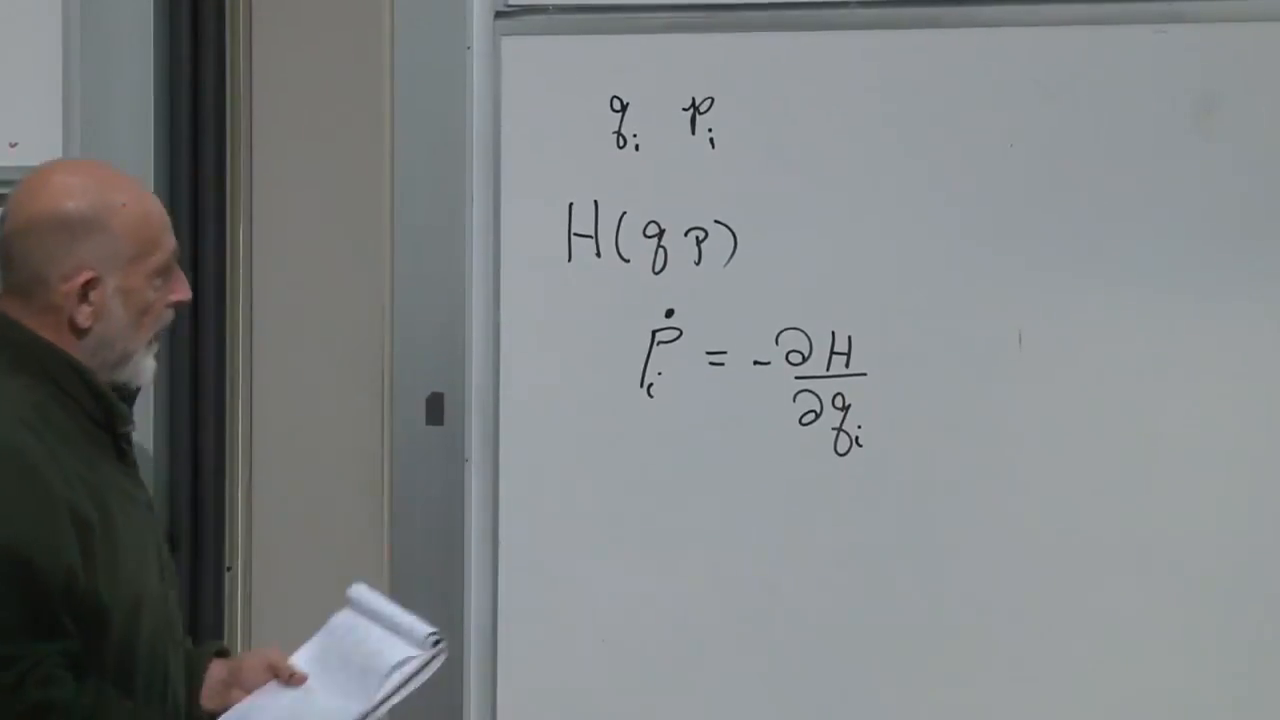
\includegraphics[width=0.82\textwidth]{lecture_07_figure_02.png}
  \caption{Kanonische Variablen, die Funktion \(H(q,p)\) und die Impulsgleichung Hamiltons zu Beginn der Wiederholung.}
  \lectureframe{00:07:29}
\end{figure}

Obwohl die Gleichungen paarweise indiziert sind, muss sich die Dynamik nicht für jedes Paar getrennt beschreiben lassen. Der Hamiltonian kann alle \(q_i\) und \(p_i\) miteinander koppeln, sodass etwa \(\dot p_1\) vom Zustand des gesamten Systems abhängen kann.

\begin{classroomqa}
  \audiencequestion{Ist die Darstellung nun axiomatisch? Welche Beziehung zwischen
  \(p\) und \(q\) wurde vorausgesetzt?
  \lecturetimestamp{00:17:08--00:18:18}}
  \lecturerresponse{Die Hamilton-Gleichungen legen die formale Theorie fest, sobald
  \(H(q,p)\) und die kanonischen Paare spezifiziert sind. Es gibt keine allgemeingültige
  zusätzliche Annahme \(p=m\dot q\). Diese Beziehung gilt für ein gewöhnliches
  kartesisches Teilchen mit quadratischer kinetischer Energie, doch andere Koordinaten und
  andere Hamilton-Funktionen führen zu anderen Impuls--Geschwindigkeits-Beziehungen. Die Gleichungen
  selbst liefern die Beziehung durch
  \(\dot q_i=\partial H/\partial p_i\). Ob ein vorgeschlagener Hamiltonian
  in der Natur realisiert ist, ist eine weitere physikalische Frage.}
\end{classroomqa}

Nun können wir die Energieerhaltung mit einer Argumentation in einer Zeile herleiten. Entlang einer Bahn lautet die totale Ableitung von \(H\)
\begin{equation}
  \frac{dH}{dt}
  =
  \sum_i\left(
    \frac{\partial H}{\partial q_i}\dot q_i
    +\frac{\partial H}{\partial p_i}\dot p_i
  \right)
  +\frac{\partial H}{\partial t}.
  \label{eq:l7-total-h-derivative}
\end{equation}
Der letzte Term beschreibt die explizite Zeitabhängigkeit bei festgehaltenen \(q\) und \(p\), etwa weil sich ein von außen vorgegebener Parameter ändert. Setzen wir Gleichung~\eqref{eq:l7-hamilton-equations} ein, erhalten wir
\begin{align}
  \frac{dH}{dt}
  &=
  \sum_i\left[
    \frac{\partial H}{\partial q_i}
    \frac{\partial H}{\partial p_i}
    -\frac{\partial H}{\partial p_i}
    \frac{\partial H}{\partial q_i}
  \right]
  +\frac{\partial H}{\partial t}\\
  &=\frac{\partial H}{\partial t}.
  \label{eq:l7-h-energy-rate}
\end{align}
Jeder Summand hebt seinen Gegenpart auf. Folglich gilt
\begin{equation}
  \frac{\partial H}{\partial t}=0
  \quad\Longrightarrow\quad
  \frac{dH}{dt}=0.
  \label{eq:l7-energy-conservation}
\end{equation}
Für ein abgeschlossenes, zeittranslationsinvariantes System ist der Hamiltonian erhalten und entspricht der Energie.

\begin{classroomqa}
  \audiencequestion{Was ändert sich, wenn der Hamiltonian explizit von der Zeit abhängt? \lecturetimestamp{00:10:32--00:12:33}}
  \lecturerresponse{Dann gilt Gleichung~\eqref{eq:l7-h-energy-rate} weiterhin, doch die Energie des Teilsystems muss nicht konstant sein. Eine explizite Zeitabhängigkeit steht gewöhnlich für einen nicht berücksichtigten Antrieb, der Energie mit dem System austauscht. Wird dieser Antrieb als dynamischer Teil in ein größeres abgeschlossenes System aufgenommen, kann der Hamiltonian des Gesamtsystems wieder zeitunabhängig und dessen Gesamtenergie erhalten sein.}
\end{classroomqa}

\section{Energie als Geometrie im Phasenraum}

Nehmen wir nun an, \(H\) habe keine explizite Zeitabhängigkeit. Die Anfangsbedingung legt einen Wert \(E\) fest, und der Phasenraumpunkt bleibt auf
\begin{equation}
  H(q,p)=E.
  \label{eq:l7-energy-surface}
\end{equation}
Der Phasenraum hat \(2n\) Dimensionen. An regulären Punkten definiert eine Gleichung unter seinen Koordinaten eine Hyperfläche der Dimension \((2n-1)\). Verschiedene Werte von \(E\) ergeben verschiedene Hyperflächen. Sie müssen weder geschlossen noch kompakt sein; die Energieerhaltung besagt lediglich, dass eine Bahn, die auf einer solchen Fläche beginnt, sie nie verlässt.

Für den angepassten harmonischen Oszillator aus der vorangegangenen Vorlesung gilt
\begin{equation}
  H=\frac{\omega}{2}(p^2+q^2).
  \label{eq:l7-oscillator-hamiltonian}
\end{equation}
Jede Menge konstanter Energie ist also ein Kreis,
\begin{equation}
  p^2+q^2=\frac{2E}{\omega}.
  \label{eq:l7-oscillator-circle}
\end{equation}

\begin{figure}[htbp]
  \centering
  \includegraphics[width=0.84\textwidth]{lecture_07_figure_04.png}
  \caption{Die Phasenraumskizze der Dimension \(2n\) und der Hamiltonian des harmonischen Oszillators, mit denen Flächen konstanter Energie eingeführt werden.}
  \lectureframe{00:15:20}
\end{figure}

Die Bewegungsgleichungen
\begin{equation}
  \dot q=\omega p,\qquad \dot p=-\omega q,
  \label{eq:l7-oscillator-flow}
\end{equation}
lassen den Punkt im Uhrzeigersinn um seinen Kreis laufen. Die Energiegleichung gibt an, auf welcher Kurve die Bewegung verläuft; Hamiltons Gleichungen bestimmen Richtung und Geschwindigkeit entlang dieser Kurve.

\begin{figure}[htbp]
  \centering
  \begin{tikzpicture}[scale=0.95]
    \draw[->] (-2.7,0) -- (2.7,0) node[right] {\(q\)};
    \draw[->] (0,-2.7) -- (0,2.7) node[above] {\(p\)};
    \draw[thick] (0,0) circle (0.8);
    \draw[thick] (0,0) circle (1.5);
    \draw[thick] (0,0) circle (2.2);
    \draw[->,very thick] (0,2.2) arc[start angle=90,end angle=40,radius=2.2];
    \draw[->,very thick] (1.5,0) arc[start angle=0,end angle=-50,radius=1.5];
    \draw[->,very thick] (0,-0.8) arc[start angle=-90,end angle=-140,radius=0.8];
  \end{tikzpicture}
  \caption{Konstante Energie ergibt die Kreise; die Oszillatorgleichungen liefern das tangentiale Strömungsfeld im Uhrzeigersinn.}
\end{figure}

\begin{classroomqa}
  \audiencequestion{Sind Hamiltons beide Gleichungen und \(H=E\) verschiedene Fassungen derselben Gleichung?
  \lecturetimestamp{00:15:53--00:17:06}}
  \lecturerresponse{Nein. Hamiltons Gleichungen sind die beiden Bewegungsgesetze erster Ordnung für ein kanonisches Paar. Sie implizieren \(dH/dt=0\), woraus \(H=E\) folgt. Der Wert von \(E\) wird durch die Anfangsbedingung festgelegt. Die Gleichung \(H=E\) bestimmt eine Fläche; für sich genommen legt sie die Geschwindigkeit entlang dieser Fläche nicht fest.}
\end{classroomqa}

\section{Von einem Zustand zu einem Fluss von Zuständen}

Statt einer einzelnen Anfangsbedingung zu folgen, verteilen wir alle möglichen Anfangsbedingungen über den Phasenraum und lassen die Zeit verstreichen. Jeder Punkt ist ein vollständiger möglicher Zustand, und jeder Zustand entwickelt sich gemäß Hamiltons Gleichungen. Man kann sich diese Verteilung als Staub oder als imaginäres Fluid vorstellen. Dabei wird keine materielle Substanz in den Phasenraum gegossen; das Fluid ist eine Veranschaulichung, mit der sich alle Bahnen zugleich erfassen lassen.

Das Geschwindigkeitsfeld im Phasenraum ist
\begin{equation}
  \mathbf V(q,p,t)
  =
  (\dot q_1,\ldots,\dot q_n,\dot p_1,\ldots,\dot p_n).
  \label{eq:l7-phase-velocity}
\end{equation}
Für ein kanonisches Paar schreiben wir
\begin{equation}
  V_q=\dot q=\frac{\partial H}{\partial p},
  \qquad
  V_p=\dot p=-\frac{\partial H}{\partial q}.
  \label{eq:l7-phase-components}
\end{equation}
An jedem Punkt ordnet der Hamiltonian einen Vektor zu, der dem Phasenraumpunkt seine nächste Bewegungsrichtung vorgibt. Ist \(H\) zeitunabhängig, ist das Vektorfeld stationär: Kehrt man zum selben Phasenraumpunkt zurück, erhält man dieselbe Geschwindigkeit. Hängt \(H\) von der Zeit ab, ändert sich auch das Vektorfeld mit der Zeit, doch es ist zu jedem Zeitpunkt definiert.

\begin{figure}[htbp]
  \centering
  \includegraphics[width=0.84\textwidth]{lecture_07_figure_05.png}
  \caption{Das Geschwindigkeitsfeld des harmonischen Oszillators. Die Vektoren sind tangential zu den Kreisen und werden zum Ursprung hin kürzer.}
  \lectureframe{00:24:50}
\end{figure}

Beim harmonischen Oszillator dreht sich jeder Radius mit der Winkelgeschwindigkeit \(\omega\). Punkte nahe dem Ursprung haben eine geringere lineare Geschwindigkeit, weil sie in derselben Periode einen kürzeren Kreis durchlaufen. Der gesamte Staub rotiert daher wie ein starrer Kreisel.

\begin{classroomqa}
  \audiencequestion{Bedeutet die starre Rotation, dass alle Bahnen des Oszillators dieselbe Periode haben? \lecturetimestamp{00:21:10--00:21:42}}
  \lecturerresponse{Ja. Diese Amplitudenunabhängigkeit ist die definierende besondere Eigenschaft des harmonischen Oszillators. Jeder Kreis wird mit derselben Kreisfrequenz \(\omega\) durchlaufen, obwohl der Betrag der Geschwindigkeit im Phasenraum auf einem kleineren Kreis geringer ist.}
\end{classroomqa}

\begin{classroomqa}
  \audiencequestion{Ist die Geschwindigkeit im Phasenraum an jedem Punkt gleich?
  \lecturetimestamp{00:24:29--00:25:37}}
  \lecturerresponse{Nein. Sowohl ihre Richtung als auch ihr Betrag ändern sich im Allgemeinen mit dem Ort. Beim Oszillator ist der Vektor tangential zum jeweiligen Kreis und hat den Betrag \(\omega\sqrt{p^2+q^2}\). Ein Vektorfeld bedeutet, dass jedem Punkt ein Vektor zugeordnet ist, nicht dass überall derselbe Vektor steht.}
\end{classroomqa}

\begin{classroomqa}
  \audiencequestion{Was genau sind die Teilchen und die Dichte dieses imaginären Fluids? \lecturetimestamp{00:56:03--00:58:40}}
  \lecturerresponse{Jeder Punkt steht für einen vollständigen Zustand des gesamten mechanischen Systems, nicht für ein einzelnes physisches Teilchen. Fünf Teilchen, die sich in einer Raumdimension bewegen, erfordern fünf Orts- und fünf Impulskoordinaten, also einen zehn-dimensionalen Phasenraum; in drei Dimensionen sind es dreißig Dimensionen. Der Staub ist ein Ensemble alternativer Zustände. Wenn das Fluidbild ablenkt, kann man stattdessen einfach ein Gebiet von Anfangsbedingungen nehmen, jeden Punkt darin entwickeln und sein Phasenraumvolumen vorher und nachher vergleichen.}
\end{classroomqa}

\section{Kompression und Divergenz}

Um zu fragen, ob dieses imaginäre Fluid Volumen verliert, betrachten wir zunächst eine Dimension. Punkte auf einer Geraden bewegen sich mit der Geschwindigkeit \(v(x)\). Zwei benachbarte Punkte im Abstand \(\delta x\) haben einen Geschwindigkeitsunterschied
\begin{equation}
  \delta v \simeq \frac{dv}{dx}\,\delta x.
  \label{eq:l7-one-dimensional-strain}
\end{equation}
Ist \(dv/dx>0\), bewegt sich der vordere Punkt schneller und das Intervall wird gedehnt. Ist \(dv/dx<0\), wird es komprimiert. Eine stationäre inkompressible Strömung in einer Dimension erfüllt daher
\begin{equation}
  \frac{dv}{dx}=0.
  \label{eq:l7-one-dimensional-incompressible}
\end{equation}

\begin{figure}[htbp]
  \centering
  \includegraphics[width=0.84\textwidth]{lecture_07_figure_06.png}
  \caption{Die eindimensionale Herleitung von \(dv/dx\) als lokaler Dehnungs- oder Kompressionsrate.}
  \lectureframe{00:30:20}
\end{figure}

Es gibt zwei gleichwertige Sichtweisen. Man kann einem materiellen Intervall folgen und fragen, ob sich seine Länge ändert. Oder man kann ein kleines Intervall festhalten und fragen, ob pro Zeiteinheit genauso viel hineinfließt wie hinaus. Bei der ersten Sichtweise folgt man dem Fluid, bei der zweiten beobachtet man, wie es vorbeiströmt.

In mehr als einer Dimension kann sich ein Gebiet entlang einer Achse dehnen und entlang einer anderen komprimieren, ohne dass sich sein Gesamtvolumen ändert. Für ein Geschwindigkeitsfeld \(\mathbf V=(V_x,V_y,V_z)\) ist die relevante lokale Rate die Divergenz,
\begin{equation}
  \nabla\cdot\mathbf V
  =
  \frac{\partial V_x}{\partial x}
  +\frac{\partial V_y}{\partial y}
  +\frac{\partial V_z}{\partial z}.
  \label{eq:l7-spatial-divergence}
\end{equation}
Eine positive Divergenz bedeutet lokale Expansion, eine negative lokale Kontraktion; Inkompressibilität liegt vor, wenn
\begin{equation}
  \nabla\cdot\mathbf V=0.
  \label{eq:l7-zero-divergence}
\end{equation}
Gleicher Zu- und Abfluss durch eine festgehaltene kleine Box ist dieselbe lokale Aussage wie die Erhaltung des Volumens einer mitbewegten kleinen Box.

\begin{figure}[htbp]
  \centering
  \includegraphics[width=0.86\textwidth]{lecture_07_figure_07.png}
  \caption{Eine zweidimensionale Box, ihre Strömungskomponenten und die Summe der Ableitungen nach den jeweils zugehörigen Koordinaten, die die Divergenz definiert.}
  \lectureframe{00:35:30}
\end{figure}

\begin{classroomqa}
  \audiencequestion{Geht es um ein Fluid im gewöhnlichen Raum oder um eine Strömung im Phasenraum? \lecturetimestamp{00:34:27--00:34:40}}
  \lecturerresponse{Das Divergenzargument ist zunächst ein allgemeines Argument über Fluide. Wir wenden es auf den gerade-dimensionalen Phasenraum an, dessen Koordinatenrichtungen die \(q_i\) und \(p_i\) und dessen Geschwindigkeitskomponenten die \(\dot q_i\) und \(\dot p_i\) sind.}
\end{classroomqa}

Kehren wir nun zu den diskreten Zustandsabbildungen zurück. In einem umkehrbaren Zyklus führt ein Pfeil in jeden Knoten hinein und einer aus ihm heraus; eine ausgewählte Zustandsmenge enthält bei ihrer Entwicklung weiterhin gleich viele Elemente. In einem Senkenpunkt führen viele Pfeile hinein und zu wenige hinaus; mehrere Alternativen werden ununterscheidbar.

\begin{figure}[htbp]
  \centering
  \includegraphics[width=0.80\textwidth]{lecture_07_figure_08.png}
  \caption{Die diskrete Senke, mit der sich die Divergenz wieder an den Test für umkehrbare Gesetze aus der ersten Vorlesung anknüpfen lässt.}
  \lectureframe{00:40:15}
\end{figure}

Die kontinuierliche Frage lässt sich nun präzise stellen: Hat der Hamiltonsche Fluss Divergenz null, sodass ein kleines Gebiet unterscheidbarer Zustände niemals zu einem kleineren Phasenraumvolumen zusammengedrückt wird?

\section{Der Satz von Liouville}

\begin{theorem}[Liouville's theorem]Für ein glattes Hamiltonsches System hat das kanonische Geschwindigkeitsfeld im Phasenraum Divergenz null:
\begin{equation}
  \sum_i\left(
    \frac{\partial\dot q_i}{\partial q_i}
    +\frac{\partial\dot p_i}{\partial p_i}
  \right)=0.
  \label{eq:l7-liouville-divergence}
\end{equation}Äquivalent dazu erhält die Hamiltonsche Entwicklung das kanonische Phasenraumvolumenelement \(dq_1\cdots dq_n\,dp_1\cdots dp_n\).
\end{theorem}

\begin{classroomqa}
  \audiencequestion{Sind die Komponenten namens \(V\) einfach die Zeitableitungen von \(p\) und \(q\)? \lecturetimestamp{00:42:20--00:43:22}}
  \lecturerresponse{Ja. Für ein Paar gilt \(V_q=\dot q\) und \(V_p=\dot p\). Ordnet man alle diese Ableitungen passend an, erhält man den Geschwindigkeitsvektor des Flusses im vollständigen Phasenraum.}
\end{classroomqa}

Für ein kanonisches Paar folgen aus Hamiltons Gleichungen
\begin{equation}
  V_p=-\frac{\partial H}{\partial q},
  \qquad
  V_q=\frac{\partial H}{\partial p}.
  \label{eq:l7-liouville-components}
\end{equation}
Damit lautet die Divergenz
\begin{align}
  \frac{\partial V_p}{\partial p}
  +\frac{\partial V_q}{\partial q}
  &=
  -\frac{\partial}{\partial p}
    \left(\frac{\partial H}{\partial q}\right)
  +\frac{\partial}{\partial q}
    \left(\frac{\partial H}{\partial p}\right)\\
  &=
  -\frac{\partial^2H}{\partial p\,\partial q}
  +\frac{\partial^2H}{\partial q\,\partial p}
  =0.
  \label{eq:l7-liouville-proof}
\end{align}

\begin{figure}[htbp]
  \centering
  \includegraphics[width=0.86\textwidth]{lecture_07_figure_09.png}
  \caption{Das Rechteck mit endlichen Differenzen veranschaulicht, weshalb sich glatte gemischte partielle Ableitungen vertauschen lassen.}
  \lectureframe{00:47:30}
\end{figure}

Die Gleichheit gemischter partieller Ableitungen lässt sich anhand von vier benachbarten Punkten \(A,B,C,D\) an den Ecken eines kleinen Rechtecks in der \(q\)-\(p\)-Ebene veranschaulichen. Bildet man zunächst die Differenz nach \(q\) und anschließend die nach \(p\), ergibt sich bis auf die beiden kleinen Seitenlängen
\begin{equation}
  F(B)+F(D)-F(A)-F(C).
  \label{eq:l7-finite-difference-combination}
\end{equation}
Bildet man die Differenzen in umgekehrter Reihenfolge, erhält man dieselbe Kombination. Im Grenzfall eines kleinen Rechtecks ergibt sich
\(\partial_p\partial_qF=\partial_q\partial_pF\), sofern die erforderlichen Ableitungen stetig sind.

\begin{figure}[htbp]
  \centering
  \includegraphics[width=0.88\textwidth]{lecture_07_figure_10.png}
  \caption{Die kanonische Divergenz, nachdem Hamiltons Gleichungen sie auf zwei gemischte Ableitungen mit entgegengesetzten Vorzeichen zurückgeführt haben.}
  \lectureframe{00:50:20}
\end{figure}

Bei vielen Freiheitsgraden erfolgt dieselbe Aufhebung für jedes kanonische Paar:
\begin{align}
  \sum_i\left(
    \frac{\partial\dot p_i}{\partial p_i}
    +\frac{\partial\dot q_i}{\partial q_i}
  \right)
  &=
  \sum_i\left(
    -\frac{\partial^2H}{\partial p_i\,\partial q_i}
    +\frac{\partial^2H}{\partial q_i\,\partial p_i}
  \right)\\
  &=0.
  \label{eq:l7-many-pair-proof}
\end{align}
Die Dehnung in einer kanonischen Richtung wird durch die Kompression in der zu ihr konjugierten Richtung ausgeglichen. Diese paarweise Aufhebung ist eine stärkere Struktur als eine zufällige Aufhebung zwischen nicht zusammengehörigen Achsen.

\begin{classroomqa}
  \audiencequestion{Wird die Summe über alle kanonischen Paare mitverstanden?
  \lecturetimestamp{00:52:00--00:52:36}}
  \lecturerresponse{Ja. Gleichung~\eqref{eq:l7-many-pair-proof} wird über \(i\) summiert, und die beiden gemischten Ableitungen heben sich für jedes \(q_i,p_i\)-Paar einzeln auf.}
\end{classroomqa}

\begin{classroomqa}
  \audiencequestion{Sieht die dargestellte Divergenz nach einer kartesischen Darstellung aus. Gilt der Satz auch nach einem Koordinatenwechsel?
  \lecturetimestamp{00:52:50--00:53:22,\allowbreak\ 00:58:18--00:58:40}}
  \lecturerresponse{Die natürliche Formulierung verwendet kanonische Koordinaten und das kanonische Volumenelement \(dq_1\cdots dq_n\,dp_1\cdots dp_n\). Eine kanonische, also symplektische Transformation ändert Koordinaten und Impulse gemeinsam und erhält dieses Volumen. Bei beliebigen nichtkanonischen Koordinaten muss ein Jacobi-Faktor in das Volumenmaß eingehen; das naive Produkt der Koordinatendifferentiale muss nicht invariant sein.}
\end{classroomqa}

\begin{classroomqa}
  \audiencequestion{Erfordert der Satz von Liouville einen zeitunabhängigen Hamiltonian? \lecturetimestamp{00:53:43--00:55:51}}
  \lecturerresponse{Nein. Für die Energieerhaltung war \(\partial H/\partial t=0\) erforderlich, doch im Beweis der Divergenz wird nur nach \(q_i\) und \(p_i\) bei festgehaltener Zeit abgeleitet. Für \(H(q,p,t)\) heben sich die gemischten Ableitungen weiterhin auf. Ein zeitabhängiger Hamiltonian erzeugt daher einen zeitabhängigen, aber zu jedem Zeitpunkt volumenbewahrenden kanonischen Fluss.}
\end{classroomqa}

\section{Was Volumenerhaltung bedeutet und was nicht}

Nehmen wir ein beliebiges kleines Gebiet \(R_0\) von Anfangsbedingungen und entwickeln jeden Punkt darin um eine Zeit \(t\) weiter. Der Satz von Liouville besagt
\begin{equation}
  \operatorname{Vol}(R_t)=\operatorname{Vol}(R_0).
  \label{eq:l7-volume-preservation}
\end{equation}
Das Gebiet kann sich verschieben, drehen, scheren und zu einem langen Filament dehnen. Geschützt ist sein Volumen, nicht seine Form. Bei einer glatten Hamiltonschen Entwicklung in endlicher Zeit können verschiedene Phasenraumpunkte nicht zusammenfallen.

Für endliche Zeiten ist ein glatter Hamiltonscher Fluss eine invertierbare Abbildung mit einer glatten Umkehrabbildung, die durch Rückwärtsentwicklung entsteht. Damit lässt sich auch die im Unterricht aufgestellte Behauptung erklären, dass ein zusammenhängender Klumpen nicht in getrennte Stücke zerreißen kann: Der Fluss verformt das Gebiet kontinuierlich und erhält seine Topologie, auch wenn ein extrem dünner Hals bei endlicher Auflösung zwei Lappen getrennt erscheinen lassen kann.

\begin{figure}[htbp]
  \centering
  \includegraphics[width=0.86\textwidth]{lecture_07_figure_12.png}
  \caption{Mögliche Verformungen eines Phasenraumgebiets. Ein glatter Hamiltonscher Fluss kann einen dünnen Hals erzeugen, aber das Gebiet in endlicher Zeit nicht tatsächlich in unabhängig entwickelte Stücke zerreißen.}
  \lectureframe{01:04:55}
\end{figure}

\begin{classroomqa}
  \audiencequestion{Kann ein Phasenraumgebiet abschnüren und in zwei Stücke zerfallen? \lecturetimestamp{01:04:10--01:05:49}}
  \lecturerresponse{Nicht unter einem glatten deterministischen Hamiltonschen Fluss in endlicher Zeit. An einem hypothetischen Abschnürungspunkt gibt es weiterhin einen Phasenraumpunkt mit einer zugeordneten Geschwindigkeit, nicht zwei unvereinbare Richtungen. Das Gebiet kann ein sehr langes, schmales Verbindungsfilament entwickeln, doch die Entwicklung bleibt eineindeutig und zerreißt es nicht.}
\end{classroomqa}

\begin{classroomqa}
  \audiencequestion{Sind zwei weit voneinander entfernte Lappen eines gedehnten Klumpens physisch verbunden oder quantenverschränkt?
  \lecturetimestamp{01:08:01--01:09:16}}
  \lecturerresponse{Eine solche physische Verbindung ist damit nicht gemeint. Der Klumpen ist eine Menge alternativer Anfangsbedingungen, kein einzelnes materielles Objekt. Ihn als ein Gebiet zu bezeichnen, hält fest, dass die Zustände aus derselben gemeinsamen Menge hervorgegangen sind; über Kräfte oder Quantenverschränkung zwischen ihnen sagt das nichts aus.}
\end{classroomqa}

\begin{classroomqa}
  \audiencequestion{Was geschieht nahe dem aufrechten instabilen Gleichgewicht eines starren Pendels? Überlagern sich Bewegungen im Uhrzeigersinn und gegen den Uhrzeigersinn?
  \lecturetimestamp{01:07:07--01:07:47}}
  \lecturerresponse{Benachbarte Anfangsbedingungen können sich auf sehr unterschiedliche Bahnen auseinanderentwickeln und so die beschriebenen dünnen Filamente bilden. Sie werden nicht zu demselben Phasenraumpunkt: Das Vorzeichen der infinitesimalen Auslenkung oder des Impulses unterscheidet die beiden Seiten. Für den exakt ausgeglichenen Zustand ist die Bewegung eindeutig bestimmt; im idealen Modell bleibt er im Gleichgewicht.}
\end{classroomqa}

\subsection{Expansion im Ortsraum und Kontraktion im Impulsraum}

Wenn eine kanonische Transformation einen Ortsbereich um den Faktor \(a\) ausdehnt, verkleinert sich die Skala des konjugierten Impulses um den reziproken Faktor:
\begin{equation}
  q\longrightarrow aq,
  \qquad
  p\longrightarrow \frac{p}{a},
  \qquad
  dq\,dp\longrightarrow dq\,dp.
  \label{eq:l7-canonical-scaling}
\end{equation}
Das ist der klare Phasenrauminhalt des Beispiels mit der Gasexpansion. Bei einer adiabatischen Expansion wächst der zugängliche Bereich im gewöhnlichen Raum, während typische Impulse abnehmen und das Gas abkühlt. Eine genaue thermodynamische Beziehung hängt von der Dimension, dem Expansionsprotokoll und den Wechselwirkungen ab; der Satz von Liouville liefert die Volumenbedingung, nicht jeden thermodynamischen Koeffizienten.

\begin{classroomqa}
  \audiencequestion{Gilt dieselbe Argumentation auch für ein expandierendes Universum, selbst bei einer plötzlichen Expansion? \lecturetimestamp{00:53:23--00:56:00}}
  \lecturerresponse{Der Satz von Liouville gilt immer dann, wenn die vollständige Dynamik Hamiltonsch ist, auch bei explizit zeitabhängigen kanonischen Variablen. Eine Expansion in Ortsrichtungen muss von der entsprechenden Kontraktion in kanonischen Impulsrichtungen begleitet sein. Die kosmologische Skalenexpansion, die kontrollierte Expansion eines Gases und eine frei explodierende Wolke sind jedoch nicht derselbe physikalische Prozess. Eine Hubble-ähnliche Korrelation zwischen Abstand und Fluchtgeschwindigkeit kann entstehen, weil sich schnellere Objekte weiter bewegen, während adiabatische Abkühlung die Kontraktion der lokalen Impulsverteilung betrifft. Der Satz schränkt in beiden Fällen die vollständige Abbildung im Phasenraum ein.}
\end{classroomqa}

\begin{classroomqa}
  \audiencequestion{Welchen praktischen Nutzen hat der Satz von Liouville?
  \lecturetimestamp{01:06:16--01:07:04}}
  \lecturerresponse{Er ist für die statistische Mechanik zentral. Er bestimmt, wie sich Ensembles mikroskopischer Zustände entwickeln, und liegt der Beziehung zwischen Phasenraumvolumen und Entropie zugrunde. Die Expansion und Abkühlung eines Gases ist ein unmittelbares Beispiel; später wird der Satz zu einem grundlegenden Werkzeug für Überlegungen zum Gleichgewicht und Nichtgleichgewicht.}
\end{classroomqa}

\section{Ein Fluss, der die Form stark verändert}

Der harmonische Oszillator erhält sowohl Fläche als auch Form, weil sein Fluss eine starre Drehung ist. Das ist ein Sonderfall. Um Volumenerhaltung von Starrheit zu unterscheiden, betrachten wir
\begin{equation}
  H=\lambda pq,
  \label{eq:l7-pq-hamiltonian}
\end{equation}
wobei \(\lambda\) die Einheit einer inversen Zeit hat. In der Vorlesung wird \(\lambda=1\) gesetzt; wenn wir es beibehalten, bleiben die Dimensionen ausdrücklich sichtbar.

\begin{figure}[htbp]
  \centering
  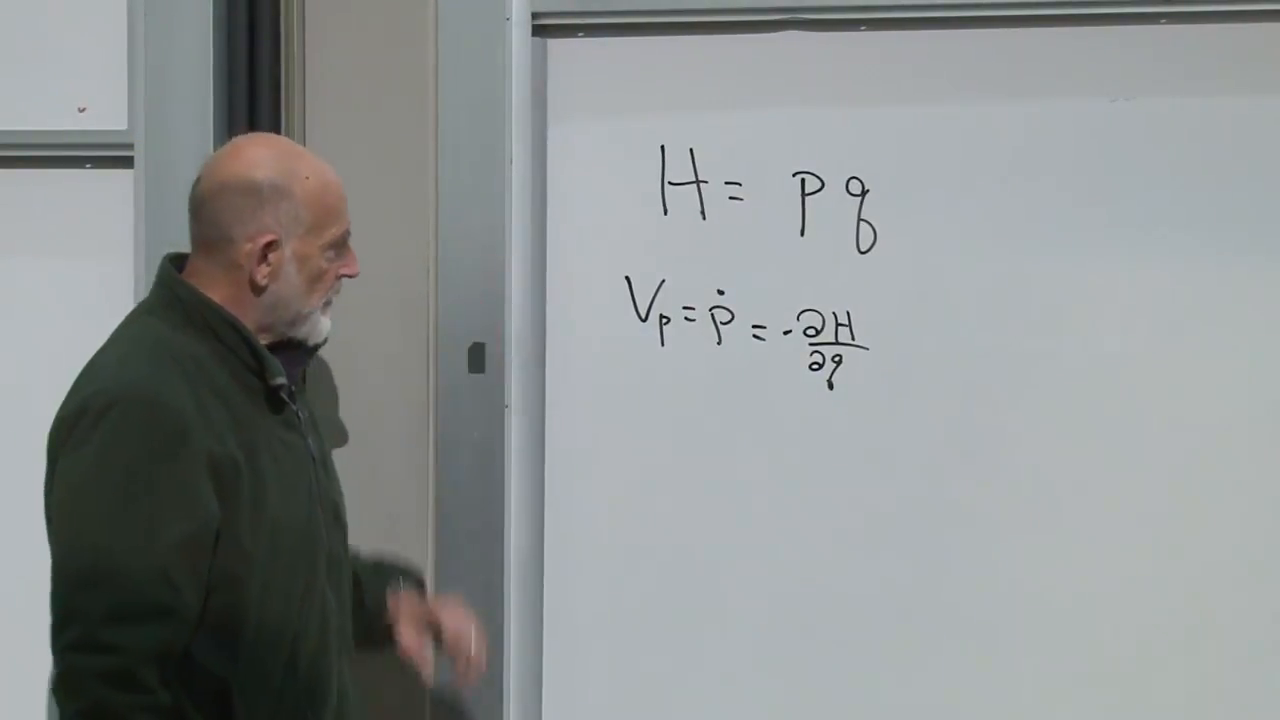
\includegraphics[width=0.82\textwidth]{lecture_07_figure_03.png}
  \caption{Beginn des Beispiels mit \(H=pq\) und erste Komponente der Geschwindigkeit im Phasenraum.}
  \lectureframe{01:00:11}
\end{figure}

Hamiltons Gleichungen lauten
\begin{equation}
  \dot p=-\lambda p,
  \qquad
  \dot q=\lambda q,
  \label{eq:l7-pq-flow}
\end{equation}
mit den Lösungen
\begin{equation}
  p(t)=p_0e^{-\lambda t},
  \qquad
  q(t)=q_0e^{\lambda t}.
  \label{eq:l7-pq-solutions}
\end{equation}
Ein quadratisches Gebiet wird in \(p\) exponentiell gestaucht und um denselben Faktor in \(q\) gedehnt:
\begin{equation}
  \Delta p(t)\Delta q(t)
  =
  \Delta p(0)\Delta q(0).
  \label{eq:l7-pq-area}
\end{equation}
Die Divergenz bestätigt das Ergebnis lokal,
\begin{equation}
  \frac{\partial\dot p}{\partial p}
  +\frac{\partial\dot q}{\partial q}
  =-\lambda+\lambda=0.
  \label{eq:l7-pq-divergence}
\end{equation}

\begin{figure}[htbp]
  \centering
  \includegraphics[width=0.86\textwidth]{lecture_07_figure_11.png}
  \caption{Ein kompaktes Gebiet wird zu einem langen, dünnen Streifen gedehnt, während der Fluss mit \(H=pq\) die Fläche erhält.}
  \lectureframe{01:02:10}
\end{figure}

\begin{classroomqa}
  \audiencequestion{Da \(pq\) die Einheit einer Wirkung hat, bedeutet der Satz von Liouville dann die Erhaltung der Wirkung? \lecturetimestamp{01:03:00--01:04:09}}
  \lecturerresponse{Nein. Der Satz besagt die Erhaltung des Phasenraumvolumens. Bei einem kanonischen Paar hat \(dq\,dp\) die Einheit einer Wirkung; diese Dimensionsbeziehung deutet die Quantenmechanik an, in der Phasenraumzellen in Einheiten gemessen werden, die durch \(\hbar\) festgelegt sind. Das Produkt \(pq\) ist jedoch weder selbst Hamiltons Wirkungsfunktional noch automatisch ein Drehimpuls, nur weil die Einheiten übereinstimmen.}
\end{classroomqa}

Das Beispiel zeigt außerdem, dass Winkel nicht erhalten bleiben müssen. Ein rechtwinkliges Kreuz mit ungleichen Komponenten wird durch die Skalierung in Gleichung~\eqref{eq:l7-pq-solutions} in seiner metrischen Gestalt geschert, während die Fläche erhalten bleibt. Der Satz von Liouville ist ein Flächen- oder Volumensatz, kein Satz über gewöhnliche euklidische Starrheit.

\section{Dämpfung erzeugt eine Senke}

Um zu sehen, was der Satz ausschließt, betrachten wir die reduzierte Gleichung für einen gedämpften Oszillator,
\begin{equation}
  m\ddot x=-kx-c\dot x,
  \qquad c>0.
  \label{eq:l7-damped-newton}
\end{equation}
Sei \(p=m\dot x\). Dann gilt
\begin{equation}
  \dot x=\frac{p}{m},
  \qquad
  \dot p=-kx-\frac{c}{m}p.
  \label{eq:l7-damped-first-order}
\end{equation}
Ohne Dämpfung umläuft der Phasenraumpunkt den Ursprung. Mit Dämpfung wird Energie auf die mikroskopischen Freiheitsgrade des umgebenden Mediums übertragen, und die Bahn windet sich spiralförmig nach innen.

\begin{figure}[htbp]
  \centering
  \includegraphics[width=0.84\textwidth]{lecture_07_figure_13.png}
  \caption{Die Gleichung des gedämpften Oszillators und seine nach innen verlaufende Spirale in der \(x\)-\(p\)-Ebene.}
  \lectureframe{01:13:30}
\end{figure}

Die Divergenz dieses reduzierten zweidimensionalen Flusses ist
\begin{equation}
  \frac{\partial\dot x}{\partial x}
  +\frac{\partial\dot p}{\partial p}
  =
  0-\frac{c}{m}<0.
  \label{eq:l7-damped-divergence}
\end{equation}
Jedes Gebiet endlicher Ausdehnung schrumpft. Der Ursprung ist ein Senkenpunkt, das kontinuierliche Gegenstück zur Zustandsabbildung, in die viele Pfeile hineinführen.

\begin{figure}[htbp]
  \centering
  \includegraphics[width=0.88\textwidth]{lecture_07_figure_14.png}
  \caption{Die Geschwindigkeitskomponenten des gedämpften Flusses im Phasenraum, aus denen die negative Divergenz \(-c/m\) folgt.}
  \lectureframe{01:16:05}
\end{figure}

Das bedeutet nicht, dass die mikroskopische Mechanik den Satz von Liouville verletzt. Die beiden Variablen \(x,p\) lassen die ungeheuer vielen Freiheitsgrade der Umgebung außer Acht, die die Energie des Oszillators aufnehmen. Das erweiterte System aus Oszillator und Umgebung kann Hamiltonsch sein und das Volumen erhalten, obwohl seine reduzierte Beschreibung in den Variablen \(x,p\) kontrahiert.

\begin{classroomqa}
  \audiencequestion{Wird der gedämpfte Oszillator weiterhin durch die Newton-Gleichung beschrieben, obwohl er in diesem reduzierten Phasenraum nicht Hamiltonsch ist?
  \lecturetimestamp{01:20:09--01:21:12}}
  \lecturerresponse{Ja. Die Newton-Gleichung \(F=ma\) kann eine empirisch vorgegebene Widerstandskraft enthalten. Die elementare \(L=T-V\)- und Hamilton-Beschreibung gilt unmittelbar für konservative Kräfte; allgemeinere Lagrangefunktionen erfassen auch einige geschwindigkeitsabhängige Kräfte. Ein Markovscher Reibungsterm für ein isoliertes Paar \(x,p\) beschreibt jedoch reduzierte dissipative Dynamik und kein abgeschlossenes kanonisches Hamilton-System.}
\end{classroomqa}

\begin{classroomqa}
  \audiencequestion{Geht wirklich Information verloren, wenn sich die gedämpften Gleichungen mit unendlicher Genauigkeit rückwärts integrieren lassen?
  \lecturetimestamp{01:25:16--01:27:17}}
  \lecturerresponse{Für jede endliche Zeit hat die ideale Differentialgleichung weiterhin eine Umkehrung; exakte Daten lassen sich also rückwärts entwickeln. Die präzise Aussage lautet, dass endliche Phasenraumzellen exponentiell schrumpfen. Um ihren früheren Zustand wiederherzustellen, ist daher exponentiell zunehmende Genauigkeit erforderlich; im Grenzfall unendlicher Zeit nähern sich alle Trajektorien dem Senkenpunkt. Dies ist die nächstliegende kontinuierliche klassische Analogie zum diskreten Bild des Verlusts von Alternativen, aber keine Behauptung, zwei exakte Lösungen würden sich zu endlicher Zeit buchstäblich vereinigen.}
\end{classroomqa}

\begin{classroomqa}
  \audiencequestion{Kann ein Vektorfeld eine verschwindende Divergenz haben, ohne aus einem Hamilton-System hervorzugehen? \lecturetimestamp{01:18:21--01:22:34}}
  \lecturerresponse{Gewiss. Die Hamilton-Form ist hinreichend für eine verschwindende Divergenz, aber nicht notwendig. Ein beliebiges inkompressibles Geschwindigkeitsfeld kann eine verschwindende Divergenz haben, ohne auf demselben Raum ein kanonisches Hamiltonsches Vektorfeld zu sein. Das dreidimensionale Geschwindigkeitsfeld einer inkompressiblen Flüssigkeit ist das Lehrbuchbeispiel: Drei Koordinaten können für sich genommen keine kanonischen Paare bilden. Die vollständige Fluidmechanik kann zwar anspruchsvollere Hamilton-Formulierungen mit unendlich vielen Freiheitsgraden besitzen, doch ändert das nichts an der hier behaupteten einseitigen Implikation.}
\end{classroomqa}

\section{Weitere durch Fragen verdeutlichte Unterscheidungen}

\begin{classroomqa}
  \audiencequestion{Wie hängt die Bewegung auf einer Fläche konstanter Energie mit der Erhaltung eines ganzen Phasenraumvolumens zusammen?
  \lecturetimestamp{01:28:47--01:30:41}}
  \lecturerresponse{Beides sind unabhängige Folgen der Hamilton-Struktur. Ist \(H\) zeitunabhängig, bleibt jede Trajektorie auf ihrer eigenen Energiefläche. Ein endlicher Bereich kann viele solcher Flächen durchqueren; der Satz von Liouville besagt, dass das Volumen dieses gesamten Bereichs erhalten bleibt. Beim harmonischen Oszillator bleibt auch die Form des Bereichs erhalten, weil die Strömung eine starre Rotation ist. Der Bereich für \(H=pq\) behält dagegen nur seine Fläche, nicht seine Form.}
\end{classroomqa}

\begin{classroomqa}
  \audiencequestion{Welche Rolle spielt die mechanische Arbeit in der Hamilton-Beschreibung? \lecturetimestamp{01:30:44--01:32:57}}
  \lecturerresponse{Arbeit beschreibt Energie, die über eine gewählte Systemgrenze übertragen wird. Ein äußerer Akteur kann ein Gewicht anheben oder einen Parameter ändern und dadurch die Energie des Teilsystems verändern; die von ihm zugeführte Energie verliert der Akteur. Werden beide Seiten in ein einziges abgeschlossenes Modell aufgenommen, stehen wieder die Erhaltung der Gesamtenergie und der Austausch zwischen Teilsystemen im Vordergrund.}
\end{classroomqa}

\begin{classroomqa}
  \audiencequestion{Erhält die Volumenerhaltung auch die Topologie und die Winkel?
  \lecturetimestamp{01:33:00--01:33:37}}
  \lecturerresponse{Eine glatte Hamiltonsche Strömung zu endlicher Zeit erhält die Topologie, da sie eine umkehrbare stetige Verformung ist. Euklidische Winkel oder die Form bleiben im Allgemeinen nicht erhalten. Bei der Rotation des Oszillators ist das zwar der Fall, doch die Streckung für \(H=pq\) zeigt, warum dies ein Sonderfall ist.}
\end{classroomqa}

\begin{classroomqa}
  \audiencequestion{Wurde die Legendre-Transformation ausgelassen, weil sie keine physikalische Bedeutung hat? \lecturetimestamp{01:33:43--01:34:48}}
  \lecturerresponse{Nein. Sie ist die nützliche Transformation, die die Geschwindigkeitsbeschreibung in eine Impulsbeschreibung überführt und bei regulärer Abbildung \(H=\sum_i p_i\dot q_i-L\) ergibt. Die Konstruktion wurde bereits wiederholt verwendet, auch wenn ihr formaler Name nicht hervorgehoben wurde; die ausführliche allgemeine Theorie wird für den vorliegenden Satz einfach nicht benötigt.}
\end{classroomqa}

\section{Poisson-Klammern: die nächste Verdichtung}

In den letzten Minuten kehren wir zum historischen Thema zurück. Die Mechanik des 19. Jahrhunderts suchte wiederholt nach kompakten Strukturen, die scheinbar unterschiedliche Systeme miteinander verbanden---Mechanik und geometrische Optik, Teilchen und Strahlen, klassische Trajektorien und wellenartige Beschreibungen. Poisson-Klammern sind eine weitere solche Struktur und werden in der Quantenmechanik besonders wichtig.

Sei \(F(q,p)\) eine beliebige Funktion auf dem Phasenraum. Sie kann eine Koordinate, ein Impuls, das Produkt \(qp\) oder der Drehimpuls sein. Entlang der Bewegung gilt
\begin{equation}
  \frac{dF}{dt}
  =
  \sum_i\left(
    \frac{\partial F}{\partial q_i}\dot q_i
    +\frac{\partial F}{\partial p_i}\dot p_i
  \right).
  \label{eq:l7-f-time-derivative}
\end{equation}
Setzt man die Hamilton-Gleichungen ein, erhält man
\begin{equation}
  \frac{dF}{dt}
  =
  \sum_i\left(
    \frac{\partial F}{\partial q_i}
    \frac{\partial H}{\partial p_i}
    -
    \frac{\partial F}{\partial p_i}
    \frac{\partial H}{\partial q_i}
  \right).
  \label{eq:l7-f-hamiltonian-derivative}
\end{equation}

\begin{figure}[htbp]
  \centering
  \includegraphics[width=0.88\textwidth]{lecture_07_figure_15.png}
  \caption{Die Kettenregel für die Zeitableitung einer allgemeinen Phasenraumfunktion \(F(q,p)\).}
  \lectureframe{01:42:40}
\end{figure}

Die wiederholt auftretende antisymmetrische Kombination verdient einen eigenen Namen. Für zwei beliebige Funktionen \(F\) und \(G\) definieren wir ihre Poisson-Klammer durch
\begin{equation}
  \boxed{
  \{F,G\}
  =
  \sum_i\left(
    \frac{\partial F}{\partial q_i}
    \frac{\partial G}{\partial p_i}
    -
    \frac{\partial F}{\partial p_i}
    \frac{\partial G}{\partial q_i}
  \right).}
  \label{eq:l7-poisson-bracket}
\end{equation}

\begin{figure}[htbp]
  \centering
  \includegraphics[width=0.86\textwidth]{lecture_07_figure_16.png}
  \caption{Die Ableitungskombination zweier Funktionen, aufgefasst als Poisson-Klammer.}
  \lectureframe{01:44:15}
\end{figure}

Gleichung~\eqref{eq:l7-f-hamiltonian-derivative} wird zu
\begin{equation}
  \boxed{\frac{dF}{dt}=\{F,H\}.}
  \label{eq:l7-hamiltonian-poisson-evolution}
\end{equation}
Hängt \(F\) zusätzlich explizit von der Zeit ab, kommt \(\partial F/\partial t\) hinzu. Für \(F=q_i\) oder \(F=p_i\) erhält man wieder die beiden Hamilton-Gleichungen; Gl.~\eqref{eq:l7-hamiltonian-poisson-evolution} ist somit eine kompakte Form der vollständigen Dynamik.

Die Notation lässt sich immer künstlich verdichten---man könnte viele Gleichungen quadrieren, addieren und das Ergebnis eine einzige Gleichung nennen. Damit würde man die Struktur verbergen, statt sie sichtbar zu machen. Die Poisson-Klammer ist aus dem entgegengesetzten Grund nützlich: Ihre Algebra ordnet die zeitliche Entwicklung, Erhaltungsgrößen und Symmetrien. Als Nächstes entwickeln wir diese Algebra und wenden sie dann auf den Drehimpuls an, dessen Struktur sowohl in der klassischen Mechanik als auch in der Quantentheorie zentral sein wird.

\section{Die kontinuierliche Bedeutung der Umkehrbarkeit}

Wir können die Gedankenkette nun vollständig formulieren. Die Hamilton-Gleichungen erhalten \(H\), wenn der Hamiltonian nicht explizit von der Zeit abhängt; einzelne Trajektorien bleiben daher auf Energiehyperflächen konstanten Energiewerts. Dieselben Gleichungen ordnen jedem Punkt des Phasenraums eine Geschwindigkeit zu. Die Divergenz dieses Geschwindigkeitsfelds verschwindet, weil sich gemischte partielle Ableitungen paarweise aufheben. Folglich bleibt das kanonische Volumen eines ganzen Zustandsraums erhalten.

Das ist die kontinuierliche Version von einem Pfeil hinein und einem Pfeil hinaus. Die Form kann sich ändern, Winkel können sich ändern, und benachbarte Trajektorien können sich enorm voneinander entfernen. Was in einer glatten, abgeschlossenen Hamilton-Beschreibung nicht geschehen kann, ist die Kompression einer endlichen Menge von Alternativen auf ein kleineres Phasenraumvolumen. Die Strömung für \(H=pq\) zeigt, dass Streckung möglich ist; der reduzierte gedämpfte Oszillator veranschaulicht die Senke, die auftritt, sobald die Hamilton-Bedingungen aufgegeben werden. Die Poisson-Klammern verdichten dieselbe Dynamik schließlich zu der Aussage, dass der Hamiltonian jede Zeitableitung erzeugt.

\chapter{Poisson-Klammern, Erzeuger und Drehimpuls}

\lectureoverview{Die Poisson-Klammer ist mehr als eine kompakte Schreibweise für die Hamilton-Gleichungen. Sie ist eine algebraische Operation, die Transformationen erzeugt. Die Klammerung mit dem Hamiltonian erzeugt die Zeitentwicklung, die mit dem Impuls Translationen und die mit dem Drehimpuls Drehungen. In dieser Sprache werden Symmetrie und Erhaltung zu zwei Lesarten derselben verschwindenden Klammer. Wir entwickeln diesen Gedanken am harmonischen Oszillator und nutzen anschließend die Drehimpulsalgebra, um die gyroskopische Präzession herzuleiten, ohne Euler-Winkel einzuführen.}

\section{Eine Funktion entlang einer Hamiltonschen Trajektorie}

Sei \[
  F=F(q_1,\ldots,q_n,p_1,\ldots,p_n)
\] eine hinreichend differenzierbare Funktion auf dem Phasenraum. Man kann sie auf zwei Arten betrachten. Erstens ordnet sie jedem Punkt des Phasenraums eine Zahl zu. Zweitens wird sie, sobald eine Hamiltonsche Trajektorie gewählt ist, zu einer Funktion der Zeit, weil sich der Punkt \((q(t),p(t))\) bewegt. Entlang dieser Trajektorie gilt \begin{equation}
  \frac{dF}{dt}
  =
  \sum_i\left(
    \frac{\partial F}{\partial q_i}\dot q_i
    +\frac{\partial F}{\partial p_i}\dot p_i
  \right).
  \label{eq:l8-chain-rule}
\end{equation} Die Hamilton-Gleichungen \begin{equation}
  \dot q_i=\frac{\partial H}{\partial p_i},
  \qquad
  \dot p_i=-\frac{\partial H}{\partial q_i},
  \label{eq:l8-hamilton-equations}
\end{equation} führen zu \begin{equation}
  \frac{dF}{dt}
  =
  \sum_i\left(
    \frac{\partial F}{\partial q_i}
    \frac{\partial H}{\partial p_i}
    -
    \frac{\partial F}{\partial p_i}
    \frac{\partial H}{\partial q_i}
  \right).
  \label{eq:l8-fdot-expanded}
\end{equation} Die rechte Seite tritt in der klassischen Mechanik häufig auf, auch wenn keiner ihrer beiden Einträge der Hamiltonian ist. Das legt folgende Definition nahe: \begin{equation}
  \boxed{
  \{F,G\}
  =
  \sum_i\left(
    \frac{\partial F}{\partial q_i}
    \frac{\partial G}{\partial p_i}
    -
    \frac{\partial F}{\partial p_i}
    \frac{\partial G}{\partial q_i}
  \right).}
  \label{eq:l8-poisson-definition}
\end{equation} Gleichung~\eqref{eq:l8-fdot-expanded} lautet damit \begin{equation}
  \boxed{\dot F=\{F,H\}.}
  \label{eq:l8-time-generator}
\end{equation}

\begin{classroomqa}
  \audiencequestion{Wenn der zweite Eintrag von \(H\) auf eine beliebige Funktion \(G\) geändert wird, ist die Klammer dann weiterhin die Zeitableitung von \(F\)?\lecturetimestamp{00:05:45--00:06:15}}
  \lecturerresponse{Nein. Während die Notation verallgemeinert wird, erkennt das Publikum einen wichtigen Punkt. Gleichung~\eqref{eq:l8-poisson-definition} definiert \(\{F,G\}\) für zwei beliebige Phasenraumfunktionen, aber \(\dot F=\{F,G\}\) gilt nur, wenn \(G\) der Hamiltonian ist. Ein allgemeines \(G\) erzeugt eine andere infinitesimale Transformation.}
\end{classroomqa}

Eine kleine Zeitänderung lässt sich zweckmäßig schreiben als
\begin{equation}
  \delta_t F=\epsilon\,\{F,H\}.
  \label{eq:l8-small-time-step}
\end{equation}
Diese Form nimmt das Folgende vorweg. Die Zeitentwicklung ist ein Mitglied einer größeren Familie von Transformationen, die durch Poisson-Klammern erzeugt werden.

\section{Die Algebra der Klammern}

Die Klammer lässt sich nun als eigene Art der Differenzialrechnung verwenden. Ihre Regeln folgen aus der gewöhnlichen Differentiation:
\begin{align}
  \{A,B\}&=-\{B,A\}, \label{eq:l8-antisymmetry}\\
  \{A+B,C\}&=\{A,C\}+\{B,C\}, \label{eq:l8-additivity}\\
  \{\lambda A,B\}&=\lambda\{A,B\},
    \quad \lambda\ \text{constant}, \label{eq:l8-scalar-rule}\\
  \{AB,C\}&=A\{B,C\}+\{A,C\}B. \label{eq:l8-leibniz}
\end{align}
Diese vier Zeilen drücken der Reihe nach Antisymmetrie, Additivität, Linearität bei Multiplikation mit einer Konstanten und die Leibniz-Regel aus. Phasenraumfunktionen der klassischen Mechanik sind unter der gewöhnlichen Multiplikation kommutativ; daher ist die Anordnung der gewöhnlichen Faktoren \(A\) und \(B\) in der letzten Zeile unerheblich. Für Operatoren in der Quantenmechanik gilt das nicht mehr. Aus der Antisymmetrie folgt außerdem
\begin{equation}
  \{A,A\}=0.
  \label{eq:l8-self-bracket}
\end{equation}

Für kanonische Koordinaten lauten die elementaren Klammern
\begin{equation}
  \boxed{
  \{q_i,q_j\}=0,\qquad
  \{p_i,p_j\}=0,\qquad
  \{q_i,p_j\}=\delta_{ij}.}
  \label{eq:l8-canonical-brackets}
\end{equation}
Jede Funktion, die nur von den \(q_i\) abhängt, hat mit jeder anderen Funktion, die nur von den \(q_i\) abhängt, eine verschwindende Klammer. Entsprechendes gilt für Funktionen, die nur von den \(p_i\) abhängen. Eine Klammer ist nur dann von null verschieden, wenn eine kanonische Koordinate auf ihren konjugierten Impuls trifft. Das Kronecker-Delta in Gl.~\eqref{eq:l8-canonical-brackets} hält fest, dass nur übereinstimmende Indizes zusammentreffen.

\subsection{Der harmonische Oszillator als Prüfstein}

Betrachten wir
\begin{equation}
  H=\frac{p^2}{2m}+\frac{kq^2}{2}.
  \label{eq:l8-oscillator-hamiltonian}
\end{equation}
Nun verwenden wir bewusst nur die Klammerregeln und Gl.~\eqref{eq:l8-time-generator}. Zunächst gilt
\begin{align}
  \dot q
  &=\{q,H\}\\
  &=\frac{1}{2m}\{q,p^2\}\\
  &=\frac{1}{2m}\left(p\{q,p\}+\{q,p\}p\right)\\
  &=\frac{p}{m}.
  \label{eq:l8-qdot-oscillator}
\end{align}
Der Potentialterm fällt weg, weil \(\{q,q^2\}=0\). Entsprechend gilt
\begin{align}
  \dot p
  &=\{p,H\}\\
  &=\frac{k}{2}\{p,q^2\}\\
  &=\frac{k}{2}\left(q\{p,q\}+\{p,q\}q\right)\\
  &=-kq.
  \label{eq:l8-pdot-oscillator}
\end{align}
Das Minuszeichen ergibt sich genau aus der Antisymmetrie \(\{p,q\}=-\{q,p\}=-1\). Durch Kombination der beiden Gleichungen erster Ordnung erhalten wir
\begin{equation}
  m\ddot q=-kq.
  \label{eq:l8-hooke-equation}
\end{equation}

\begin{figure}[htbp]
  \centering
  
\includegraphics[width=0.82\textwidth]{lecture_08_figure_01.png}
  \caption{Der Oszillator-Hamiltonian und die beiden Klammerberechnungen, aus denen \(\dot q=p/m\) und \(\dot p=-kq\) hervorgehen.}
  \lectureframe{00:23:20}
\end{figure}

Während der Rechnung sucht die Klasse nach einem Verb für \emph{eine Poisson-Klammer bilden} und einigt sich vorläufig auf \emph{poissonieren}. Der Scherz markiert einen echten Perspektivwechsel: Ist die Algebra erst einmal bekannt, kann man direkt mit ihr rechnen, statt jedes Ergebnis aus der Definition neu herzuleiten.

\begin{classroomqa}
  \audiencequestion{Ist diese mathematische Struktur eine Gruppe oder eine Algebra? Gibt es Inverse? \lecturetimestamp{00:23:48--00:24:16}}
  \lecturerresponse{Sie ist keine Gruppe: Die Klammeroperation liefert weder das erforderliche neutrale Element noch Inverse. Die Phasenraumfunktionen bilden eine Poisson-Algebra: Sie verfügen über gewöhnliche kommutative Multiplikation und Addition sowie über eine antisymmetrische Klammer, die der Leibniz-Regel genügt. Eine weitere Identität, die Jacobi-Identität, vervollständigt die übliche abstrakte Definition, wird in dieser Vorlesung jedoch nicht entwickelt.}
\end{classroomqa}

\begin{classroomqa}
  \audiencequestion{Wie hängen Poisson-Klammern und Quantenkommutatoren zusammen? \lecturetimestamp{00:24:18--00:25:00}}
  \lecturerresponse{Die Vorlesung gibt dazu nur einen Ausblick. Beim Übergang zur Quantenmechanik wird die klassische Klammer schematisch ersetzt durch
  \[
    \{A,B\}_{\mathrm{PB}}
    \longleftrightarrow
    \frac{1}{i\hbar}[\widehat A,\widehat B].
  \]
  Diese Zuordnung erfordert Einschränkungen hinsichtlich der Operatorordnung und Quantisierung; hier wird sie nicht als Satz verwendet.}
\end{classroomqa}

Beim Oszillator hat die Klammer lediglich die Hamilton-Gleichungen wiederhergestellt. Ihre eigentliche Stärke zeigt sich, wenn der Erzeuger eine andere Erhaltungsgröße als \(H\) ist.

\section{Der Drehimpuls aus der Rotationssymmetrie}

Zur Erinnerung: Früher im Kurs haben wir die infinitesimale Form der Noether-Konstruktion verwendet. Ändert eine kontinuierliche Symmetrie die Koordinaten gemäß
\begin{equation}
  \delta q_i=\epsilon F_i(q),
  \label{eq:l8-noether-variation}
\end{equation}
so lautet die zugehörige Erhaltungsgröße in der hier betrachteten Situation
\begin{equation}
  G=\sum_i p_iF_i(q).
  \label{eq:l8-noether-charge}
\end{equation}
Der Gesamtfaktor \(\epsilon\) kann weggelassen werden: Multipliziert man eine Erhaltungsgröße mit einer festen Zahl, ändert sich das Erhaltungsgesetz nicht.

Drehen wir ein Teilchen infinitesimal um die \(z\)-Achse. Bei der in der Vorlesung verwendeten Orientierung gilt
\begin{equation}
  \delta x=-\epsilon y,\qquad
  \delta y=\epsilon x,\qquad
  \delta z=0.
  \label{eq:l8-z-rotation}
\end{equation}
Gl.~\eqref{eq:l8-noether-charge} ergibt
\begin{equation}
  L_z=-p_xy+p_yx=xp_y-yp_x.
  \label{eq:l8-lz}
\end{equation}
Durch zyklisches Vertauschen von \(x\), \(y\) und \(z\) erhalten wir
\begin{equation}
  \boxed{\begin{aligned}
    L_x&=yp_z-zp_y,\\
    L_y&=zp_x-xp_z,\\
    L_z&=xp_y-yp_x.
  \end{aligned}}
  \label{eq:l8-angular-components}
\end{equation}
Dies sind die Komponenten von
\begin{equation}
  \boldsymbol L=\boldsymbol r\times\boldsymbol p.
  \label{eq:l8-cross-product}
\end{equation}

\begin{figure}[htbp]
  \centering
  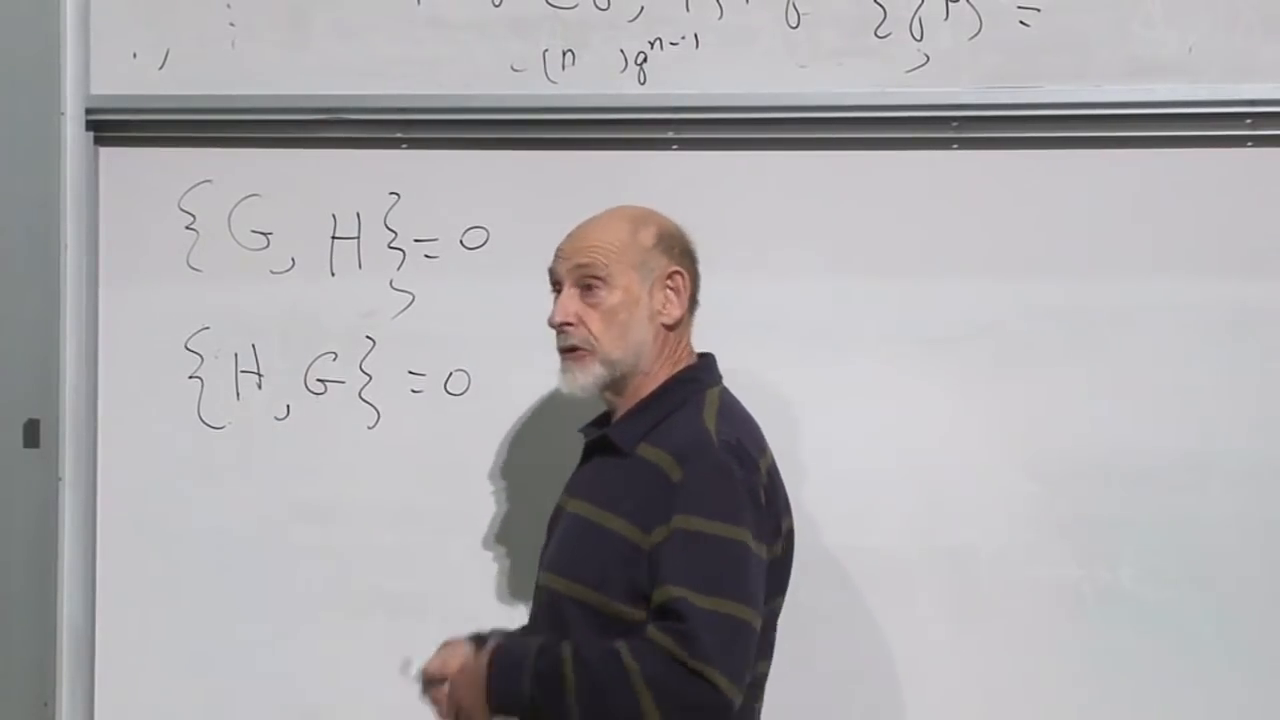
\includegraphics[width=0.82\textwidth]{lecture_08_figure_02.png}
  \caption{Die drei kartesischen Komponenten des Drehimpulses und ihre kompakte Darstellung als Kreuzprodukt.}
  \lectureframe{00:34:00}
\end{figure}

Eine Drehung um einen beliebigen Einheitsvektor \(\boldsymbol n\) wird erzeugt durch
\begin{equation}
  L_{\boldsymbol n}=\boldsymbol n\cdot\boldsymbol L.
  \label{eq:l8-arbitrary-axis}
\end{equation}
Für ein isoliertes rotationsinvariantes System sind alle drei Komponenten erhalten. Bleiben nur Drehungen um eine Achse symmetrisch, so ist nur die Komponente entlang dieser Achse sicher erhalten.

\section{Der Drehimpuls erzeugt Drehungen}

Anstatt sofort ein Problem der Rotationsdynamik zu lösen, untersuchen wir zunächst, was \(L_z\) unter der Klammer bewirkt. Mit Gl.~\eqref{eq:l8-lz} gilt
\begin{align}
  \{x,L_z\}
  &=\{x,xp_y-yp_x\}
   =-y\{x,p_x\}
   =-y,\\
  \{y,L_z\}
  &=\{y,xp_y-yp_x\}
   =x\{y,p_y\}
   =x,\\
  \{z,L_z\}&=0.
  \label{eq:l8-position-rotation-brackets}
\end{align}
Dies sind genau die Koeffizienten aus Gl.~\eqref{eq:l8-z-rotation}.

\begin{figure}[htbp]
  \centering
  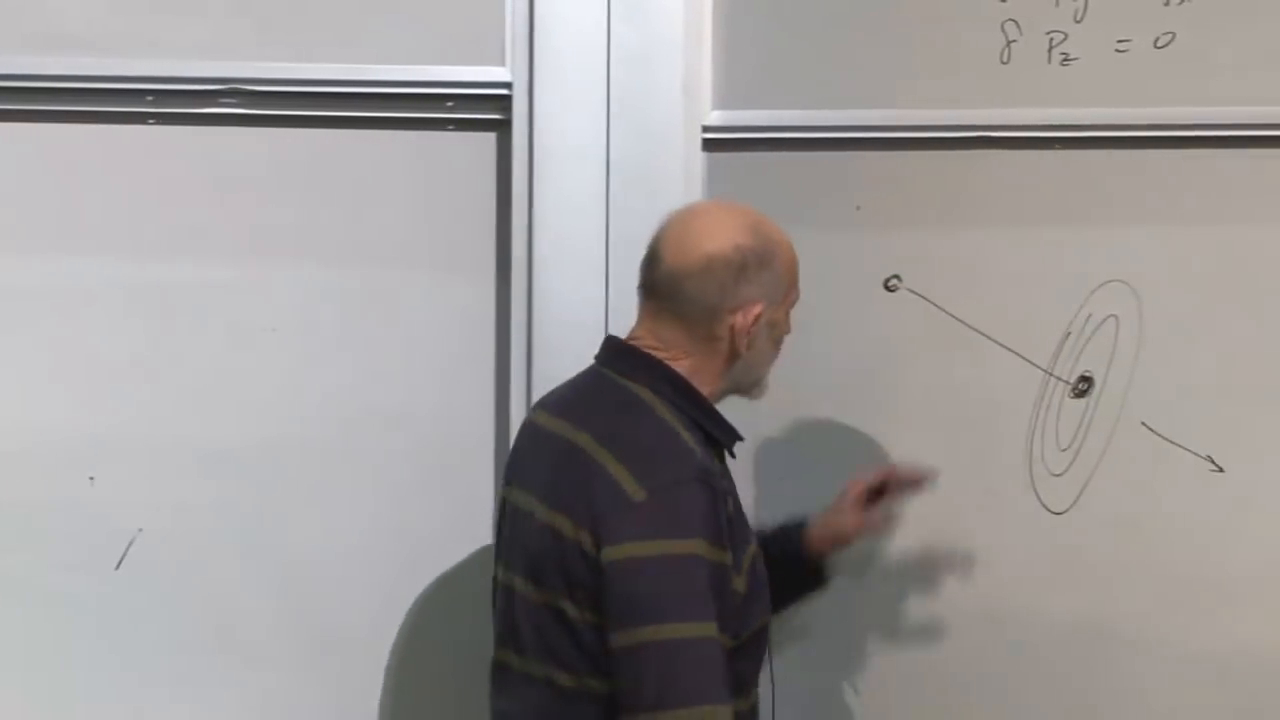
\includegraphics[width=0.82\textwidth]{lecture_08_figure_03.png}
  \caption{Die Koordinatenklammern mit \(L_z\): Die Klammer reproduziert die infinitesimale Drehung von \((x,y,z)\).}
  \lectureframe{00:38:41}
\end{figure}

Auch der Impuls ist ein Vektor, und dieselbe Rechnung ergibt
\begin{equation}
  \begin{aligned}
    \{p_x,L_z\}&=-p_y,\\
    \{p_y,L_z\}&=p_x,\\
    \{p_z,L_z\}&=0.
  \end{aligned}
  \label{eq:l8-momentum-rotation-brackets}
\end{equation}

\begin{figure}[htbp]
  \centering
  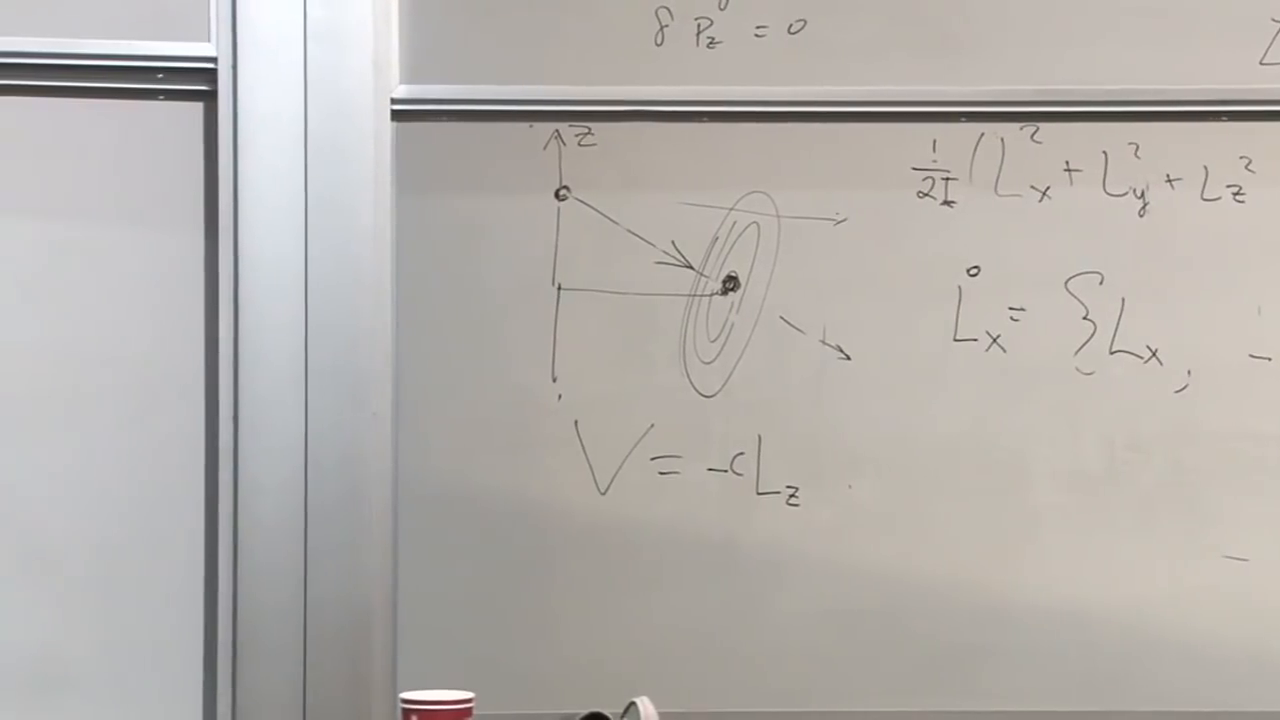
\includegraphics[width=0.82\textwidth]{lecture_08_figure_04.png}
  \caption{Ort und Impuls transformieren sich unter der von \(L_z\) erzeugten Drehung nach demselben Vektormuster.}
  \lectureframe{00:42:08}
\end{figure}

Die allgemeine Hamiltonsche Aussage lautet somit
\begin{equation}
  \boxed{\delta_G A=\epsilon\{A,G\}.}
  \label{eq:l8-generator-rule}
\end{equation}
Jede Phasenraumfunktion \(G\) definiert eine solche infinitesimale kanonische Transformation. Für \(G=L_z\) handelt es sich um eine Drehung. Für \(G=H\) ist sie ein kleiner Zeitschritt.

\begin{classroomqa}
  \audiencequestion{In der Vorlesung ist manchmal davon die Rede, das System zu drehen, und manchmal davon, die Koordinaten zu drehen. Welche Konvention gilt in den Klammergleichungen? \lecturetimestamp{00:28:22--00:29:35}}
  \lecturerresponse{Gl.~\eqref{eq:l8-z-rotation} legt die Konvention fest: Sie beschreibt die infinitesimale aktive Drehung \((x,y)\mapsto(x-\epsilon y,y+\epsilon x)\). Bei einer passiven Drehung der Achsen kehrt sich das Vorzeichen um. Ist die Konvention einmal festgelegt, sind die Klammerformeln eindeutig.}
\end{classroomqa}

\section{Der Impuls erzeugt Translationen}

Eine Translation in einer Koordinate hat die Form
\begin{equation}
  \delta q=\epsilon.
  \label{eq:l8-q-translation}
\end{equation}
Hier gilt \(F(q)=1\) in Gl.~\eqref{eq:l8-noether-variation}, daher ist die zugehörige Erhaltungsgröße \(p\). Die Behauptung, dass diese Größe die Transformation erzeugt, sagt voraus:
\begin{equation}
  \{f(q),p\}=\frac{df}{dq}.
  \label{eq:l8-translation-derivative}
\end{equation}
In der Vorlesung wird dies zunächst für Potenzen durch vollständige Induktion bewiesen. Der Induktionsanfang lautet \(\{q,p\}=1\). Es sei
\begin{equation}
  \{q^{n-1},p\}=(n-1)q^{n-2}.
  \label{eq:l8-induction-hypothesis}
\end{equation}
Dann liefert die Produktregel
\begin{align}
  \{q^n,p\}
  &=\{q\,q^{n-1},p\}\\
  &=q\{q^{n-1},p\}+\{q,p\}q^{n-1}\\
  &=(n-1)q^{n-1}+q^{n-1}\\
  &=nq^{n-1}.
  \label{eq:l8-power-translation}
\end{align}
Durch Linearität lässt sich das Ergebnis auf Polynome und konvergente Potenzreihendarstellungen erweitern. Unmittelbarer ergibt sich aus der Definition der Klammer Gl.~\eqref{eq:l8-translation-derivative} für jede differenzierbare Funktion \(f(q)\):
\begin{equation}
  \{f(q),p\}
  =
  \frac{\partial f}{\partial q}
  \frac{\partial p}{\partial p}
  =f'(q).
\end{equation}

\begin{figure}[htbp]
  \centering
  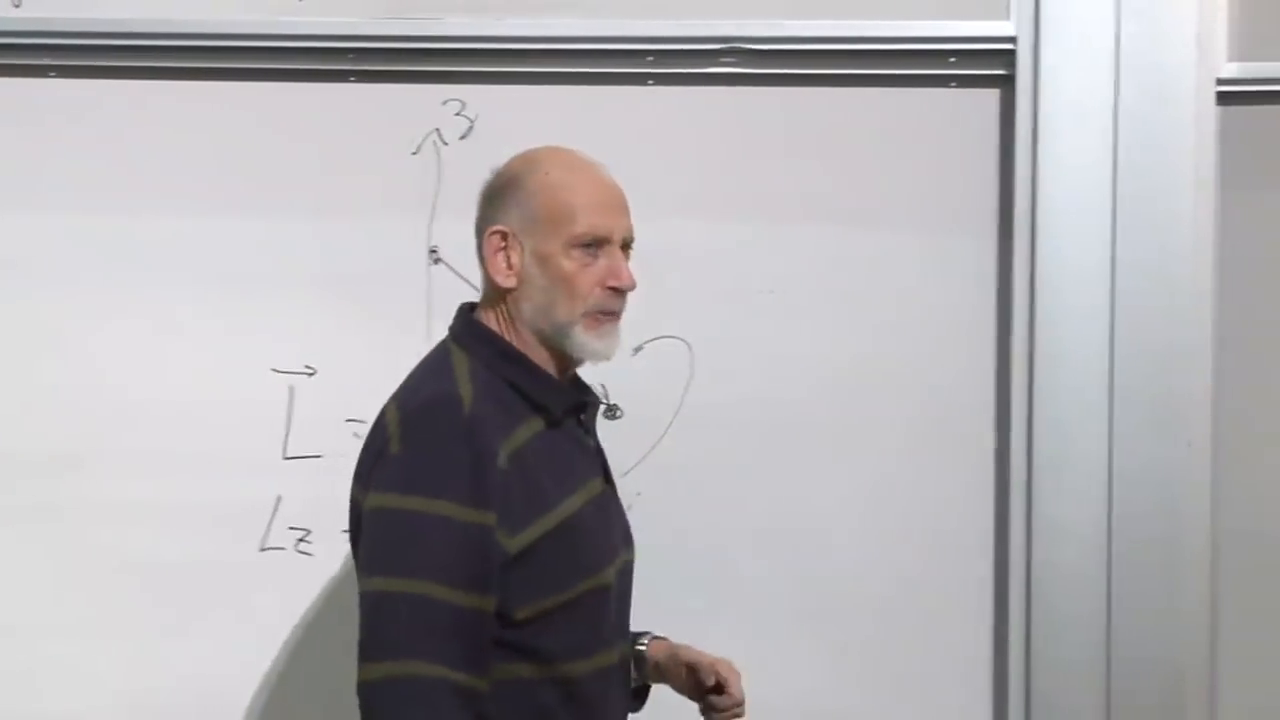
\includegraphics[width=0.82\textwidth]{lecture_08_figure_05.png}
  \caption{Das Translationsresultat nach dem Induktionsbeweis:
  \(\{F(q),p\}=dF/dq\).}
  \lectureframe{00:53:18}
\end{figure}

Wir haben nun drei Ausprägungen desselben Gedankens gesehen:
\begin{center}
  \begin{tabular}{@{}>{\raggedright\arraybackslash}p{0.37\textwidth}
                      >{\raggedright\arraybackslash}p{0.55\textwidth}@{}}
    \toprule
    Erzeuger und Transformation & Infinitesimale Wirkung\\
    \midrule
    \(H\), Zeittranslation & \(\delta_tA=\epsilon\{A,H\}\)\\
    \(p_i\), räumliche Translation & \(\delta A=\epsilon\{A,p_i\}\)\\
    \(L_i\), Drehung & \(\delta A=\epsilon\{A,L_i\}\)\\
    \bottomrule
  \end{tabular}
\end{center}
Die einer kontinuierlichen Symmetrie zugeordnete Erhaltungsgröße ist zugleich der Erzeuger dieser Symmetrie.

\section{Eine Klammer, zwei Lesarten}

Sei \(G(q,p)\) ein vorgeschlagener Erzeuger. Ist er erhalten und hängt nicht explizit von der Zeit ab, dann gilt
\begin{equation}
  \dot G=\{G,H\}=0.
  \label{eq:l8-g-conserved}
\end{equation}
Aufgrund der Antisymmetrie gilt
\begin{equation}
  \{H,G\}=0.
  \label{eq:l8-h-invariant}
\end{equation}
Die Gleichungen sind mathematisch gleichwertig, haben aber unterschiedliche physikalische Bedeutungen:
\begin{itemize}
  \item \(\{G,H\}=0\)besagt, dass \(G\) sich unter der von \(H\) erzeugten Zeitentwicklung nicht ändert.
  \item \(\{H,G\}=0\)besagt, dass \(H\) sich unter der von \(G\) erzeugten Transformation nicht ändert.
\end{itemize}
Die erste Gleichung ist ein Erhaltungsgesetz, die zweite eine Symmetrie des Hamiltonians. Noethers Zusammenhang ist in einer einzigen Null zusammengefasst.

\begin{figure}[htbp]
  \centering
  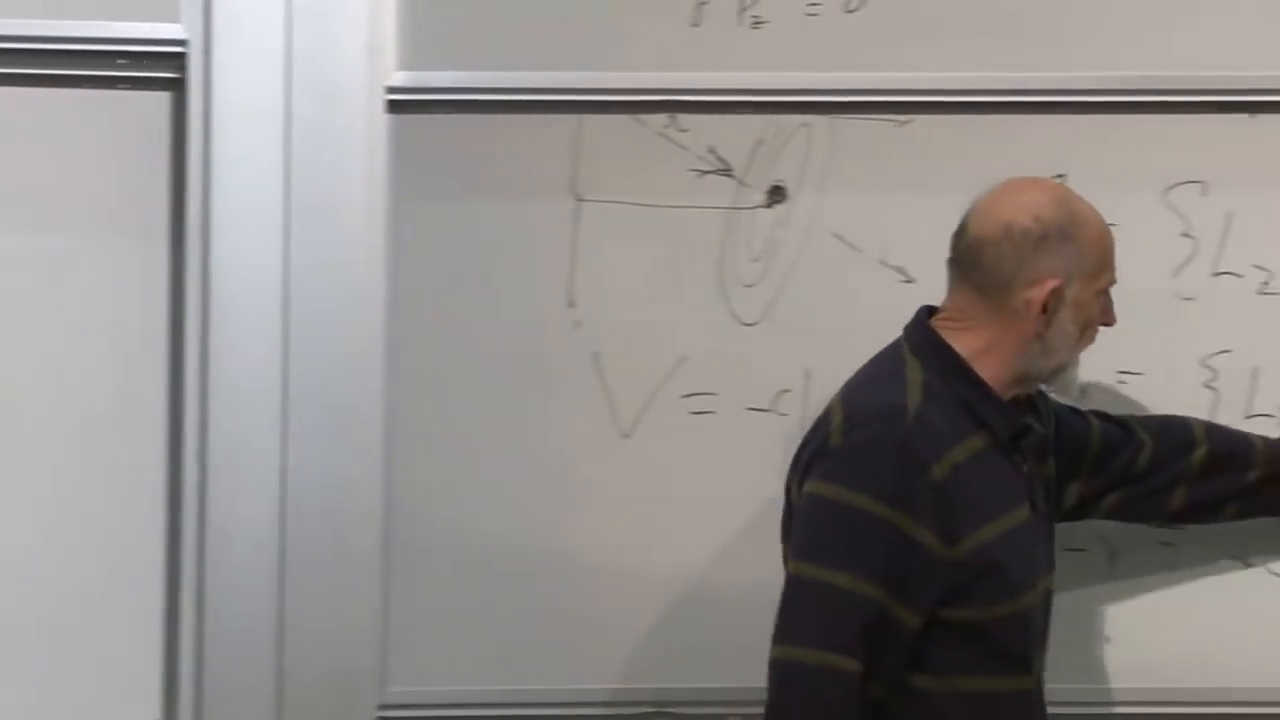
\includegraphics[width=0.82\textwidth]{lecture_08_figure_06.png}
  \caption{Die beiden Anordnungen derselben verschwindenden Klammer: Erhaltung von \(G\) und Invarianz von \(H\) unter der von \(G\) erzeugten Transformation.}
  \lectureframe{01:03:05}
\end{figure}

\begin{classroomqa}
  \audiencequestion{Lässt sich die zugehörige Symmetrie immer rekonstruieren, wenn eine Erhaltungsgröße bekannt ist? \lecturetimestamp{01:01:42--01:02:15}}
  \lecturerresponse{Im Rahmen dieser Hamiltonschen Beschreibung: ja. Man bildet die Klammer jeder Phasenraumvariablen mit \(G\). Die Gesamtheit \(\delta_GA=\epsilon\{A,G\}\) gibt an, wie sich die Variablen transformieren. Die Klammern mit \(L_z\) zeigen beispielsweise eine Drehung, selbst wenn diese Deutung zuvor nicht bekannt war. In weiterführenden Zusammenhängen können globale und Randprobleme auftreten; hier wird jedoch die lokale infinitesimale Aussage verwendet.}
\end{classroomqa}

\begin{classroomqa}
  \audiencequestion{Beschreiben diese Klammergleichungen die physikalische Bewegung, die für die Erhaltung verantwortlich ist?\lecturetimestamp{00:56:01--00:58:13}}
  \lecturerresponse{Nein. Sie identifizieren die Symmetrietransformation, nicht die tatsächliche Trajektorie. Die Erhaltung von \(L_z\) weist auf Rotationssymmetrie hin; sie besagt nicht, dass sich das Teilchen auf einer Kreisbahn bewegt. Die tatsächliche Zeitentwicklung wird von \(H\) erzeugt. Eine Klammer mit einem anderen Erzeuger beschreibt eine andere Transformationsrichtung im Phasenraum.}
\end{classroomqa}

\begin{classroomqa}
  \audiencequestion{Gibt es eine allgemeine Aussage über Transformationen, die Erhaltung nicht bereits voraussetzt? \lecturetimestamp{01:02:40--01:04:45}}
  \lecturerresponse{Ja. Gleichung~\eqref{eq:l8-generator-rule} definiert für jede Funktion \(G\) eine infinitesimale Transformation, unabhängig davon, ob sie erhalten ist. Zur Symmetrie wird sie erst, wenn der Hamiltonian invariant ist:
  \(\{H,G\}=0\). Liest man dieselbe Bedingung in umgekehrter Reihenfolge, besagt sie dann, dass \(G\) erhalten ist.}
\end{classroomqa}

\section{Die Drehimpulsalgebra}

Mit der nächsten Rechnung müssen wir die Teilchenkoordinaten nicht mehr bei jedem Rotationsproblem mitführen. Wir beginnen mit
\[
  L_x=yp_z-zp_y,\qquad
  L_z=xp_y-yp_x.
\]
In \(\{L_x,L_z\}\) verschwinden die meisten Kreuzterme, weil ihre Indizes keine kanonischen Paare bilden. Die verbleibenden Kontraktionen ergeben
\begin{align}
  \{L_x,L_z\}
  &=\{yp_z-zp_y,xp_y-yp_x\}\\
  &=xp_z-zp_x\\
  &=-L_y.
  \label{eq:l8-lx-lz}
\end{align}
Bei umgekehrter Reihenfolge entfällt das Minuszeichen. Durch zyklisches Vertauschen der Koordinaten erhalten wir
\begin{equation}
  \boxed{\begin{aligned}
    \{L_x,L_y\}&=L_z,\\
    \{L_y,L_z\}&=L_x,\\
    \{L_z,L_x\}&=L_y.
  \end{aligned}}
  \label{eq:l8-angular-algebra}
\end{equation}
In Indexschreibweise:
\begin{equation}
  \{L_i,L_j\}=\varepsilon_{ijk}L_k.
  \label{eq:l8-angular-algebra-index}
\end{equation}

\begin{figure}[htbp]
  \centering
  \includegraphics[width=0.82\textwidth]{lecture_08_figure_07.png}
  \caption{Die zyklische Poisson-Klammer-Algebra der drei Drehimpulskomponenten.}
  \lectureframe{01:10:52}
\end{figure}

Das Ergebnis hätte sich auch vorhersagen lassen. Da \(\boldsymbol L\) ein Vektor ist, muss die Klammer seiner \(x\)-Komponente mit \(L_z\) die infinitesimale Änderung dieser Komponente unter einer Drehung um die \(z\)-Achse ergeben, also \(-L_y\). Die explizite Rechnung bestätigt dieses geometrische Argument. Diese Gleichungen sind außerdem die klassischen Vorläufer der quantenmechanischen Drehimpuls-Kommutationsrelationen.

\section{Ein schnell rotierendes Gyroskop}

Betrachten wir als Anwendung ein Gyroskop: ein schnell rotierendes Schwungrad, dessen Mittelpunkt einen festen Abstand \(R\) von einem Drehpunkt hat. Der Vektor \(\boldsymbol r\) zeigt vom Drehpunkt zum Mittelpunkt des Schwungrads. Das Schwungrad dreht sich so schnell um seine Achse, dass der dominante Drehimpuls entlang dieser Richtung ausgerichtet bleibt. In der Näherung der Vorlesung gilt
\begin{equation}
  \boldsymbol L=\ell\,\boldsymbol r,
  \qquad
  L_z=\ell z,
  \label{eq:l8-L-parallel-r}
\end{equation}
Dabei wird \(\ell=L/R\) als konstant behandelt. Kleinere Drehimpulse, die mit Nutation oder einer Bewegung der Achse verbunden sind, werden zunächst vernachlässigt.

\begin{figure}[htbp]
  \centering
  \begin{tikzpicture}[scale=0.95,>=Latex]
    \coordinate (P) at (0,3.2);
    \coordinate (C) at (3.7,1.55);
    \draw[->] (0,-0.2) -- (0,4.35) node[above] {\(z\)};
    \fill (P) circle (1.7pt) node[left] {pivot};
    \draw[very thick,->] (P) -- (C)
      node[midway,above right] {\(\boldsymbol r\parallel\boldsymbol L\)};
    \fill (C) circle (1.7pt);
    \draw[dashed] (P) -- (0,1.55);
    \draw[dashed] (0,1.55) -- (C);
    \node[left] at (0,1.55) {\(z\)};
    \begin{scope}[shift={(C)},rotate=-24]
      \draw[very thick] (0,0) ellipse (0.65 and 1.35);
      \draw[thick] (0,0) ellipse (0.42 and 0.9);
    \end{scope}
    \draw[->,thick] (2.15,2.85)
      arc[start angle=140,end angle=35,radius=1.65];
  \end{tikzpicture}
  \caption{Näherung für ein schnell rotierendes Gyroskop. Der Abstand zwischen Drehpunkt und Mittelpunkt ist fest, und der dominante Drehimpuls der Rotation bleibt entlang der Achse und \(\boldsymbol r\) ausgerichtet.}
\end{figure}

\begin{figure}[htbp]
  \centering
  \includegraphics[width=0.82\textwidth]{lecture_08_figure_08.png}
  \caption{Die Tafelzeichnung des Schwungrads zusammen mit \(H_{\rm rot}=L^2/(2I)\) und der Auslöschung, die die Erhaltung von \(\boldsymbol L\) ohne Drehmoment beweist.}
  \lectureframe{01:18:54}
\end{figure}

\subsection{Ohne Schwerkraft: Warum jede Komponente konstant bleibt}

Für den vereinfachten rotationssymmetrischen Rotor gilt
\begin{equation}
  H_{\mathrm{rot}}
  =\frac{1}{2I}
  \left(L_x^2+L_y^2+L_z^2\right)
  =\frac{L^2}{2I}.
  \label{eq:l8-rotational-hamiltonian}
\end{equation}
Der Koeffizient ist \(1/(2I)\), nicht \(I/2\); dieser Fehler wird an der Tafel gemacht und korrigiert. Mit Gl.~\eqref{eq:l8-angular-algebra} gilt
\begin{align}
  \dot L_x
  &=\{L_x,H_{\mathrm{rot}}\}\\
  &=\frac{1}{2I}\left(
    2L_y\{L_x,L_y\}
    +2L_z\{L_x,L_z\}
  \right)\\
  &=\frac{1}{I}\left(L_yL_z-L_zL_y\right)=0.
  \label{eq:l8-free-lx}
\end{align}
Zyklisch entsprechend:
\begin{equation}
  \dot L_x=\dot L_y=\dot L_z=0.
  \label{eq:l8-free-angular-momentum}
\end{equation}
Der Skalar \(L^2\) hat mit jeder Komponente \(L_i\) eine verschwindende Klammer; in der Sprache dieser Algebra ist er ein Casimir. Ein drehmomentfreies Gyroskop behält somit sowohl den Betrag als auch die Richtung seines Drehimpulses bei.

\begin{classroomqa}
  \audiencequestion{Ist das Trägheitsmoment hier einfach eine Zahl?\lecturetimestamp{01:14:23--01:15:05}}
  \lecturerresponse{Für dieses reduzierte Modell: ja. Es beschreibt die Massenverteilung des Schwungrads um seine Drehachse. Ein allgemeiner starrer Körper besitzt einen Trägheitstensor und einen Rotations-Hamiltonian \(\sum_i L_i^2/(2I_i)\) in Hauptachsen. Die Vorlesung wählt den einfacheren schnell rotierenden symmetrischen Rotor, weil es darum geht, die Methode der Poisson-Klammern zu zeigen, und nicht die vollständige Dynamik starrer Körper zu entwickeln.}
\end{classroomqa}

\subsection{Schwerkraft und das Vorzeichen des Potentials}

Wir wählen die vertikale Koordinate \(z\) nach oben positiv und setzen den Drehpunkt in den Ursprung. Die gravitative potenzielle Energie des Mittelpunkts des Schwungrads ist
\begin{equation}
  V=Mgz.
  \label{eq:l8-mgz}
\end{equation}
Da \(L_z=\ell z\) gilt,
\begin{equation}
  V=cL_z,
  \qquad
  c=\frac{Mg}{\ell}=\frac{MgR}{L}.
  \label{eq:l8-potential-lz}
\end{equation}
Hier gilt \(c>0\), wenn \(\boldsymbol L\) parallel zu \(\boldsymbol r\) gewählt wird. Dreht sich das Schwungrad in die entgegengesetzte Richtung, kehrt sich die vorzeichenbehaftete Beziehung zwischen \(\boldsymbol L\) und \(\boldsymbol r\) um und damit auch die zugehörige vorzeichenbehaftete Präzessionsfrequenz.

\begin{figure}[htbp]
  \centering
  \includegraphics[width=0.82\textwidth]{lecture_08_figure_09.png}
  \caption{Die Geometrie mit fester Länge, die \(\boldsymbol L=\ell\boldsymbol r\) und \(L_z=\ell z\) zugrunde liegt.}
  \lectureframe{01:25:38}
\end{figure}

\begin{figure}[htbp]
  \centering
  \includegraphics[width=0.82\textwidth]{lecture_08_figure_10.png}
  \caption{Ein Zwischenstand an der Tafel zeigt \(V=-cL_z\). Nachdem \(z\) als nach oben positiv festgelegt ist, wird das Vorzeichen später korrigiert: Für \(\boldsymbol L=\ell\boldsymbol r\) und \(\ell>0\) ist das konsistente Ergebnis \(V=+cL_z\).}
  \lectureframe{01:22:43}
\end{figure}

\begin{classroomqa}
  \audiencequestion{Warum kann die Höhe durch eine Komponente des Drehimpulses ersetzt werden? Ist die schräge Linie eine Achse oder ein Ortsvektor?\lecturetimestamp{01:22:20--01:25:43}}
  \lecturerresponse{\(\boldsymbol r\), der Vektor vom feststehenden Drehpunkt zum Mittelpunkt des Schwungrads, ist die passendste Bezeichnung für die schräge Linie. Eine physikalische Achse kann entlang dieses Vektors liegen, doch die in der Rechnung verwendete Beziehung ist die Näherung für schnelle Rotation \(\boldsymbol L=\ell\boldsymbol r\). Daher sind ihre \(z\)-Komponenten proportional. In der Diskussion wechseln die Bezeichnungen mehrmals, bevor diese Unterscheidung feststeht.}
\end{classroomqa}

\begin{classroomqa}
  \audiencequestion{Unter welchen Annahmen ist \(\ell\) konstant, und was gilt nicht mehr, wenn der Mittelpunkt des Schwungrads radial gleiten kann?\lecturetimestamp{01:25:43--01:26:38,\allowbreak\ 01:34:22--01:35:00}}
  \lecturerresponse{Man nimmt an, dass die dominante Eigendrehung viel größer ist als der mit der langsamen Bewegung verbundene Drehimpuls und dass der Abstand zwischen Drehpunkt und Mittelpunkt fest ist. Dann ändert sich der Betrag des Eigendrehimpulses nur wenig, und \(\boldsymbol L\) dreht sich mit \(\boldsymbol r\). Könnte sich der Mittelpunkt radial verschieben, wäre \(z\) nicht mehr mit einem einzigen konstanten Koeffizienten proportional zu \(L_z\); der reduzierte Hamiltonian \(V=cL_z\) würde die Bewegung dann nicht beschreiben.}
\end{classroomqa}

\begin{classroomqa}
  \audiencequestion{Warum steht an der Tafel zunächst ein Minuszeichen und später ein Pluszeichen? Spielt die Drehrichtung eine Rolle?\lecturetimestamp{01:27:13--01:28:15,\allowbreak\ 01:33:09--01:33:21}}
  \lecturerresponse{Das anfängliche Vorzeichen ist ein Fehler an der laufenden Tafel, vermischt mit einer noch nicht festgelegten Achsenkonvention. Sobald \(z\) als nach oben positiv definiert ist, nimmt \(V=Mgz\) mit der Höhe zu. Gilt \(\boldsymbol L=\ell\boldsymbol r\) mit \(\ell>0\), so folgt \(V=+cL_z\). Eine Umkehr der Drehrichtung kehrt die vorzeichenbehaftete Proportionalität und die Präzessionsrichtung um, rechtfertigt aber keine beliebige Vorzeichenwahl.}
\end{classroomqa}

\subsection{Präzession aus drei kurzen Gleichungen}

Der vollständige reduzierte Hamiltonian lautet
\begin{equation}
  H=
  \frac{1}{2I}\left(L_x^2+L_y^2+L_z^2\right)+cL_z.
  \label{eq:l8-full-gyro-hamiltonian}
\end{equation}
Wir haben bereits gezeigt, dass \(L^2\) mit jeder Komponente \(L_i\) eine verschwindende Klammer hat. Nur der lineare Term trägt bei:
\begin{align}
  \dot L_z&=\{L_z,H\}=0,\\
  \dot L_x&=\{L_x,H\}=c\{L_x,L_z\}=-cL_y,\\
  \dot L_y&=\{L_y,H\}=c\{L_y,L_z\}=cL_x.
  \label{eq:l8-precession-equations}
\end{align}

\begin{figure}[htbp]
  \centering
  \includegraphics[width=0.82\textwidth]{lecture_08_figure_11.png}
  \caption{Die Gleichungen für die endgültigen Komponenten: \(L_z\) bleibt konstant, während \(L_x\) und \(L_y\) ineinander übergehen.}
  \lectureframe{01:30:35}
\end{figure}

Die vertikale Komponente und der Betrag der horizontalen Komponente sind konstant:
\begin{equation}
  \frac{d}{dt}(L_x^2+L_y^2)
  =2L_x(-cL_y)+2L_y(cL_x)=0.
\end{equation}
Fassen wir die horizontalen Komponenten zusammen,
\begin{equation}
  L_+=L_x+iL_y,
  \qquad
  \dot L_+=icL_+,
\end{equation}
so ergibt sich
\begin{equation}
  L_+(t)=L_+(0)e^{ict}.
  \label{eq:l8-precession-solution}
\end{equation}
Der Drehimpulsvektor präzediert somit mit der Winkelgeschwindigkeit \(|c|=MgR/L\) um die vertikale Achse. Bei dieser idealisierten gleichförmigen Bewegung bleibt seine Neigung konstant.

\begin{classroomqa}
  \audiencequestion{Wurde der Term der Rotationsenergie beim Aufstellen der Präzessionsgleichungen vernachlässigt?\lecturetimestamp{01:35:01--01:35:49}}
  \lecturerresponse{Nein. Er gehört zum vollständigen Hamiltonian, wie in Gl.~\eqref{eq:l8-full-gyro-hamiltonian}. Er trägt lediglich nichts zu \(\dot L_i\) bei, weil \(\{L_i,L^2\}=0\) gilt; diese Auslöschung wurde bereits für die drehmomentfreie Bewegung bewiesen. Die Frage eines Studenten macht diesen impliziten Schritt explizit.}
\end{classroomqa}

\begin{classroomqa}
  \audiencequestion{Ist gleichförmige Präzession ein Gleichgewicht? Was geschieht nach einem kleinen Stoß? \lecturetimestamp{01:32:38--01:33:08}}
  \lecturerresponse{Man bezeichnet sie besser als stationäre Bewegung denn als statisches Gleichgewicht. Ein kleiner Stoß führt im Allgemeinen zusätzlich zu einer Nutation, einer Schwingung des Neigungswinkels. Bei einem sehr schnell rotierenden Rad ist diese Schwingung klein; deshalb berücksichtigt die vereinfachte Behandlung nur nahezu gleichförmige Präzession.}
\end{classroomqa}

\begin{classroomqa}
  \audiencequestion{Erfordert Präzession eine Abstützung oder eine reale Achse? \lecturetimestamp{01:31:49--01:32:38,\allowbreak\ 01:33:49--01:35:00}}
  \lecturerresponse{Dieses mechanische Modell setzt einen festen Abstand zwischen Drehpunkt und Schwerpunkt voraus, sodass eine Zwangsbedingung für die Abstützung sorgt. Das tiefer liegende algebraische Ergebnis ist allgemeiner: Immer wenn ein Drehimpuls einen Hamilton-Term besitzt, der linear von einer seiner Komponenten abhängt, erzeugt dieselbe Poisson-Klammer-Algebra Präzession. Der mikroskopische Ursprung des Drehimpulses muss kein tatsächliches Rad auf einer Achse sein.}
\end{classroomqa}

\begin{classroomqa}
  \audiencequestion{Ist dies dieselbe Präzession wie die des Elektronen- oder Kernspins in einem Magnetfeld oder die Präzession der Planetenbahn? \lecturetimestamp{01:35:50--01:37:00}}
  \lecturerresponse{Ein an ein Magnetfeld gekoppeltes magnetisches Moment hat einen Hamilton-Term, der linear von einer Spin-Komponente abhängt, und gehorcht daher derselben Drehimpulsalgebra. Die Präzession des Kernspins liegt der Kernspinresonanz zugrunde. Die Präzession des Perihels einer Planetenbahn ist ein anderes Phänomen, das zufällig dieselbe Bezeichnung \emph{precession} trägt; es handelt sich nicht um dieselbe Rechnung.}
\end{classroomqa}

\begin{classroomqa}
  \audiencequestion{Ist das seitlich montierte Gyroskop im Wesentlichen dasselbe wie ein Kreisel? \lecturetimestamp{01:37:02--01:37:23}}
  \lecturerresponse{Ja. Der Unterschied liegt vor allem in der geometrischen Bezeichnung: Wenn die Drehachse seitlich aus ihrer Abstützung herausragt, spricht man gewöhnlich von einem Gyroskop; wenn sie nahezu vertikal steht, spricht man von einem Kreisel. Die Struktur von Drehimpuls und Drehmoment ist dieselbe.}
\end{classroomqa}

\section{Was die Rechnung gezeigt hat}

Es wurden keine Euler-Winkel eingeführt und auch nicht die Koordinaten sämtlicher Teile des Schwungrads verfolgt. Sobald \[
  \{L_i,L_j\}=\varepsilon_{ijk}L_k
\] bekannt war, ergaben sich die Gleichungen für die interessierenden Variablen unmittelbar. Das soll die Leistungsfähigkeit der Methode zeigen. Der Oszillator hat gezeigt, dass Poisson-Klammern vertraute Dynamik reproduzieren können. Am Drehimpuls zeigte sich, dass sie noch mehr leisten:
\begin{itemize}
  \item Eine Erhaltungsgröße erzeugt die zugehörige infinitesimale Symmetrie;
  \item die Erhaltung von \(G\) und die Invarianz von \(H\) sind zwei Lesarten von \(\{G,H\}=0\);
  \item Die Algebra der Observablen kann in sich abgeschlossen sein, sodass sich die Dynamik ohne Rückgriff auf mikroskopische Koordinaten lösen lässt;
  \item Ein Hamiltonian, der linear in einer Drehimpulskomponente ist, erzeugt eine Präzession um diese Achse.
\end{itemize}
Die Vorlesung endet, bevor die vollständigen Euler-Gleichungen für einen allgemeinen starren Körper behandelt werden. Ihre engere Schlussfolgerung ist bereits vollständig: Die passenden Erzeuger und ihre Poisson-Algebra machen Symmetrie und Bewegung mit bemerkenswerter Einfachheit sichtbar.
\chapter{Magnetische Kräfte, Vektorpotentiale und das Wirkungsprinzip}

\lectureoverview{Elektrostatische Kräfte folgen dem vertrauten konservativen Muster, magnetische Kräfte hängen jedoch von der Geschwindigkeit ab. Um sie in die Lagrange-Mechanik einzuordnen, entwickeln wir zunächst die benötigte Vektoranalysis, nutzen den quellenfreien Charakter des Magnetfelds, um ein Vektorpotential einzuführen, untersuchen dessen Eichfreiheit und konstruieren anschließend den magnetischen Term in der Wirkung.}

\section{Eine neue Art von Kraft}

Die vorangegangene Diskussion über Drehimpuls, Kreisel und Poisson-Klammern hat mehrere Themen zusammengeführt. Insbesondere präzediert ein rotierender geladener Körper in einem Magnetfeld ähnlich wie ein Kreisel. Nun wenden wir uns von dieser Analogie der Bewegung eines einzelnen geladenen Teilchens zu.

Elektrostatische Kräfte erfordern keine neue Mechanik. Ist \(U(\mathbf x)\) eine potenzielle Energie, so gilt
\begin{equation}
  \mathbf F=-\nabla U(\mathbf x),
\end{equation}
und die übliche Argumentation führt zur Erhaltung der Summe aus kinetischer und potenzieller Energie. Für ein Teilchen mit der Ladung \(e\) in einem elektrostatischen Potential \(V(\mathbf x)\) gilt
\begin{equation}
  U(\mathbf x)=eV(\mathbf x),
  \qquad
  \mathbf F_{\mathrm{el}}=-e\nabla V.
\end{equation}
Magnetische Kräfte haben eine andere Form. Sie hängen von der Geschwindigkeit des Teilchens ab und lassen sich daher nicht einfach durch Hinzufügen einer weiteren gewöhnlichen potenziellen Energie einführen. Dennoch folgen sie aus einem Wirkungsprinzip und lassen sowohl eine Lagrange- als auch eine Hamilton-Beschreibung zu. Um diese Beschreibung zu erhalten, ist ein kurzer, aber wesentlicher Einschub zur Vektoranalysis erforderlich.

\section{Felder und lokale Operationen}

\subsection{Was ein Feld festhält}

Ein Feld ordnet jedem Punkt des Raums und im Allgemeinen auch jedem Zeitpunkt eine physikalische Größe zu. Temperatur und Druck sind Skalarfelder. Die Windgeschwindigkeit ist ein Vektorfeld. Elektrische und magnetische Felder sind Vektorfelder. Andere Theorien enthalten selbst auf mikroskopischen Skalen Skalarfelder, während die Gravitation durch ein Tensorfeld beschrieben wird. Für die vorliegende Diskussion lassen wir die Zeitabhängigkeit außer Acht und schreiben Felder als Funktionen von \(\mathbf x\).

Entscheidend an einem Feld ist seine lokale Bedeutung. Stellen wir uns vor, ein bestimmter Bereich sei in einer Tasche verborgen. Um das elektrische Feld in diesem Bereich zu messen, bringen wir eine kleine Probeladung hinein und beobachten ihre Beschleunigung. Die Kraft wird durch das Feld am Aufenthaltsort der Ladung bestimmt, nicht dadurch, dass man jede weit entfernte Quelle gesondert befragt. Dasselbe gilt für ein Magnetfeld und eine bewegte Probeladung. Später werden wir dieses einfache Bild im Hinblick auf das Vektorpotential einschränken müssen, aber als Ausgangspunkt ist es richtig.

\subsection{Der Differentialoperator}

Ableitungen machen aus Feldern andere Felder. Wir fassen die drei räumlichen Ableitungen zusammen zu
\begin{equation}
  \nabla
  =
  \left(
    \frac{\partial}{\partial x},
    \frac{\partial}{\partial y},
    \frac{\partial}{\partial z}
  \right).
\end{equation}
Das Symbol wird \emph{del} oder \emph{Nabla} gelesen. Sein Aussehen wie ein umgedrehtes Dreieck ist einprägsam; seine eigentliche Bedeutung besteht jedoch darin, dass es formal wie ein Vektor behandelt werden kann, dessen Komponenten Differentialoperatoren sind.

Dies ist der gewöhnliche dreidimensionale physikalische Raum, nicht der Phasenraum und auch kein Konfigurationsraum eines Vielteilchensystems. Außerdem ist \(\nabla\) kein Vektorfeld, das für sich allein stehen könnte. Es muss auf etwas wirken. Ist \(T(\mathbf x)\) ein skalares Temperaturfeld, so ist
\begin{equation}
  \nabla T
  =
  \left(
    \frac{\partial T}{\partial x},
    \frac{\partial T}{\partial y},
    \frac{\partial T}{\partial z}
  \right)
\end{equation}
sein Gradient, also ein echtes Vektorfeld.

\begin{figure}[htbp]
\centering
\includegraphics[width=0.82\textwidth]{lecture_09_figure_01.png}
\caption{An der Tafel wird \(\nabla\) als Vektor räumlicher Differentialoperatoren eingeführt und auf ein skalares Feld \(T(\mathbf x)\) angewendet.}
\lectureframe{00:11:30}
\end{figure}

Ein Skalar ist nicht einfach eine Größe, die mit nur einer Komponente geschrieben wird. Es ist eine Größe, deren Wert unabhängig von der Orientierung der Koordinatenachsen ist. Temperatur ist das Standardbeispiel. Für ein Vektorfeld \(\mathbf E\) ist auch der lokale Ausdruck \(\mathbf E\cdot\mathbf E\) ein Skalar. Ein Potential durch Integration eines Feldes zu konstruieren, ist dagegen eine nichtlokale Operation: Dabei werden Werte entlang eines Weges verwendet.

\subsection{Divergenz}

Für ein Vektorfeld \(\mathbf A=(A_x,A_y,A_z)\) ist der Skalar
\begin{equation}
  \nabla\cdot\mathbf A
  =
  \frac{\partial A_x}{\partial x}
  +\frac{\partial A_y}{\partial y}
  +\frac{\partial A_z}{\partial z}
\end{equation}
seine Divergenz. In der Sprache der Strömungsmechanik misst eine positive Divergenz die lokale Tendenz, nach außen zu strömen, während eine negative Divergenz eine Tendenz zum Zusammenströmen misst. Eine Fluidquelle hat eine positive Divergenz, eine Senke eine negative. Dieses Bild ist qualitativ, macht aber den quellenfreien Charakter des Magnetfelds anschaulich.

\section{Kreuzprodukte, Epsilon-Symbole und Rotation}

\subsection{Das Kreuzprodukt in Komponenten}

Für zwei Vektoren \(\mathbf V\) und \(\mathbf A\) lautet eine Komponente des Kreuzprodukts
\begin{equation}
  (\mathbf V\times\mathbf A)_x
  =
  V_yA_z-V_zA_y.
\end{equation}
Die beiden anderen erhält man durch zyklisches Vertauschen von \(x\to y\to z\to x\). Es ist praktisch, \(x,y,z\) durch die Indizes \(1,2,3\) zu ersetzen. Das Kronecker-Symbol ist definiert durch
\begin{equation}
  \delta_{ij}
  =
  \begin{cases}
    1,&i=j,\\
    0,&i\ne j,
  \end{cases}
\end{equation}
und das Levi--Civita-Symbol durch
\begin{equation}
  \epsilon_{123}=\epsilon_{231}=\epsilon_{312}=1,
  \qquad
  \epsilon_{132}=\epsilon_{321}=\epsilon_{213}=-1,
\end{equation}
Dabei gilt \(\epsilon_{ijk}=0\), wenn zwei Indizes übereinstimmen. Eine zyklische Anordnung auf einer Dreistundenuhr ergibt die Pluszeichen; eine Umkehr der Richtung ergibt die Minuszeichen. Beim Vertauschen beliebiger zwei Indizes wechselt das Vorzeichen, daher ist \(\epsilon_{ijk}\) vollständig antisymmetrisch.

Wir verwenden außerdem die Summenkonvention: Ein Index, der in einem Term wiederholt auftritt, wird von \(1\) bis \(3\) summiert. Die drei Gleichungen für das Kreuzprodukt lauten dann
\begin{equation}
  (\mathbf V\times\mathbf A)_i
  =
  \epsilon_{ijk}V_jA_k.
\end{equation}
Setzen wir zum Beispiel \(i=1\), bleiben nur \((j,k)=(2,3)\) und \((3,2)\) übrig:
\begin{equation}
  (\mathbf V\times\mathbf A)_1
  =
  \epsilon_{123}V_2A_3
  +\epsilon_{132}V_3A_2
  =
  V_2A_3-V_3A_2.
\end{equation}
Die kompakte Schreibweise enthält also genau die vertraute Komponentenregel.

\subsection{Ein als antisymmetrische Matrix dargestellter Vektor}

Es gibt noch eine zweite Darstellung:
\begin{equation}
  V_iA_j-V_jA_i
  =
  \epsilon_{ijk}(\mathbf V\times\mathbf A)_k.
\end{equation}
Die linke Seite hat zwei Indizes und ist unter \(i\leftrightarrow j\) antisymmetrisch. Als Matrix hat sie die Form
\begin{equation}
  M_{ij}
  =
  \begin{pmatrix}
    0&M_{12}&M_{13}\\
    -M_{12}&0&M_{23}\\
    -M_{13}&-M_{23}&0
  \end{pmatrix}.
\end{equation}
Die Diagonaleinträge verschwinden, und das untere Dreieck ist durch das obere festgelegt. Es gibt daher drei unabhängige Komponenten.

\begin{figure}[htbp]
\centering
\includegraphics[width=0.82\textwidth]{lecture_09_figure_02.png}
\caption{Eine Komponente des Kreuzprodukts und die schematische antisymmetrische \(3\times3\)-Matrix, anhand derer sich ihre unabhängigen Einträge zählen lassen. Die Markierungen in den Feldern dienen als Gedächtnisstütze und sind keine zusätzlichen Symbole.}
\lectureframe{00:34:20}
\end{figure}

\begin{classroomqa}
\audiencequestion{Ist das Kreuzprodukt oder die Zuordnung zu einem anderen Vektor auch außerhalb von drei Dimensionen sinnvoll?}
\lecturerresponse{Das antisymmetrische Objekt mit zwei Indizes ist in jeder Dimension sinnvoll, seine Zuordnung zu einem Vektor ist jedoch eine Besonderheit des dreidimensionalen Raums. Ein Vektor in drei Dimensionen hat drei Komponenten, und eine antisymmetrische \(3\times3\)-Matrix hat drei unabhängige Komponenten. In vier Dimensionen sind es entsprechend vier beziehungsweise sechs, denn \(4(4-1)/2=6\). Das antisymmetrische Objekt existiert weiterhin und lässt sich natürlich als Zweiform auffassen, ist aber kein weiterer Vierervektor.}
\end{classroomqa}

\subsection{Rotation}

Ersetzt man \(\mathbf V\) durch \(\nabla\), erhält man die Rotation:
\begin{equation}
  (\nabla\times\mathbf A)_i
  =
  \epsilon_{ijk}\frac{\partial A_k}{\partial x_j}.
\end{equation}
In gewöhnlichen Komponenten gilt
\begin{align}
  (\nabla\times\mathbf A)_x
  &=
  \frac{\partial A_z}{\partial y}
  -\frac{\partial A_y}{\partial z},\\
  (\nabla\times\mathbf A)_y
  &=
  \frac{\partial A_x}{\partial z}
  -\frac{\partial A_z}{\partial x},\\
  (\nabla\times\mathbf A)_z
  &=
  \frac{\partial A_y}{\partial x}
  -\frac{\partial A_x}{\partial y}.
\end{align}
Während die Divergenz die lokale Ausbreitung misst, misst die Rotation die lokale Zirkulation. Eine Flüssigkeit, die sich um eine Achse dreht, hat entlang dieser Achse eine von null verschiedene Rotation. Bei Geschwindigkeitsfeldern ist dieses Bild besonders anschaulich, doch die Definition gilt für jedes Vektorfeld.

\section{Zwei strukturelle Identitäten}

Zwei Tatsachen übernehmen fast die gesamte mathematische Arbeit:
\begin{equation}
  \nabla\cdot(\nabla\times\mathbf A)=0,
  \qquad
  \nabla\times(\nabla s)=0.
\end{equation}
Die erste folgt daraus, dass die zweiten Ableitungen symmetrisch sind, während \(\epsilon_{ijk}\) antisymmetrisch ist:
\begin{equation}
  \nabla\cdot(\nabla\times\mathbf A)
  =
  \epsilon_{ijk}\partial_i\partial_j A_k
  =0.
\end{equation}
Die zweite folgt aus der Vertauschbarkeit gemischter partieller Ableitungen:
\begin{equation}
  \bigl[\nabla\times(\nabla s)\bigr]_i
  =
  \epsilon_{ijk}\partial_j\partial_k s
  =0.
\end{equation}

\begin{figure}[htbp]
\centering
\includegraphics[width=0.80\textwidth]{lecture_09_figure_03.png}
\caption{Die erste Identität an der Tafel: Die Divergenz jeder Rotation verschwindet.}
\lectureframe{00:38:26}
\end{figure}

Das sind die einfachen Richtungen, passend zu den angekündigten Hausaufgaben oder zum Kurztest in der Vorlesung. Die Umkehrungen erfordern mehr Sorgfalt. Lokal oder global auf einem geeigneten einfach zusammenhängenden beziehungsweise kontrahierbaren Gebiet gilt
\begin{align}
  \nabla\cdot\mathbf F=0
  &\quad\Longrightarrow\quad
  \mathbf F=\nabla\times\mathbf A,\\
  \nabla\times\mathbf F=0
  &\quad\Longrightarrow\quad
  \mathbf F=\nabla s.
\end{align}
Ohne diese Einschränkung des Gebiets können Löcher und andere globale topologische Eigenschaften die Schlussfolgerungen verhindern. Die Vorlesung verwendet die lokale Form, die für das Folgende genau ausreicht.

\section{Warum das Magnetfeld eine Rotation ist}

\subsection{Keine beobachteten magnetischen Quellen}

Ein Magnetfeld \(\mathbf B\) wird operationell über seine Wirkung auf geladene Teilchen und Ströme definiert. In der gewöhnlichen Elektromagnetik ohne magnetische Monopole gilt
\begin{equation}
  \nabla\cdot\mathbf B=0.
\end{equation}
Das unterscheidet es vom elektrischen Feld, dessen Divergenz proportional zur elektrischen Ladungsdichte ist. Elektrische Ladungen sind Quellen und Senken des elektrischen Flusses. Isolierte Quellen oder Senken des magnetischen Flusses wurden nicht beobachtet.

Magnetische Monopole würden diese Gleichung ändern. Vereinheitlichte Feldtheorien liefern oft theoretische Gründe, solche Objekte zu erwarten. Falls sie existieren, könnten sie jedoch zu massereich sein, um mit verfügbaren Experimenten erzeugt zu werden. Die vorliegende Theorie geht daher von einer verschwindenden magnetischen Ladungsdichte aus.

\begin{classroomqa}
\audiencequestion{Was wäre ein magnetischer Monopol? Gewöhnliche Magnete haben doch bereits Nord- und Südpole.}
\lecturerresponse{Ein isolierter Monopol wäre eine echte Quelle oder Senke des Magnetfelds, analog zu einer elektrischen Ladung. Ein gewöhnlicher Stabmagnet ist etwas anderes. Die Feldlinien, die in der Nähe seines Nordpols austreten, verlaufen durch den Raum und kehren am Südpol zurück; anschließend setzen sie sich durch das Material des Magneten fort. Was von außen wie eine Quelle und eine Senke aussieht, ist miteinander verbunden – wie eine Flüssigkeit, die durch ein verborgenes Rohr strömt. Es wird kein magnetischer Fluss netto erzeugt oder vernichtet.}
\end{classroomqa}

\begin{figure}[htbp]
\centering
\includegraphics[width=0.76\textwidth]{lecture_09_figure_04.png}
\caption{Die Tafel stellt scheinbare Nord- und Südquellen gegenüber und verbindet ihre Feldlinien durch den Magneten. So wird hervorgehoben, dass der magnetische Fluss dort weder beginnt noch endet.}
\lectureframe{00:44:56}
\end{figure}

Da \(\mathbf B\) divergenzfrei ist, können wir nach dem Umkehrsatz zumindest lokal schreiben:
\begin{equation}
  \boxed{\mathbf B=\nabla\times\mathbf A}.
\end{equation}
Das Feld \(\mathbf A\) heißt Vektorpotential. Zunächst mag es wie eine unnötige Neudarstellung des messbaren Feldes \(\mathbf B\) wirken. Sein Zweck wird erst deutlich, wenn wir die Wirkung konstruieren.

\subsection{Das Vektorpotential ist nicht eindeutig}

Ist \(\mathbf A\) ein Vektorpotential, so ist auch
\begin{equation}
  \mathbf A'=\mathbf A+\nabla s
\end{equation}
eines, denn
\begin{equation}
  \nabla\times\mathbf A'
  =
  \nabla\times\mathbf A+\nabla\times(\nabla s)
  =
  \mathbf B.
\end{equation}
Diese Ersetzung ist eine \emph{Eichtransformation}. Das Magnetfeld ist eichinvariant.

\begin{figure}[htbp]
\centering
\includegraphics[width=0.80\textwidth]{lecture_09_figure_05.png}
\caption{An der Tafel stehen die definierende Beziehung \(\mathbf B=\nabla\times\mathbf A\) und die Eichverschiebung \(\mathbf A'=\mathbf A+\nabla s\) nebeneinander.}
\lectureframe{01:03:01}
\end{figure}

Man spricht es \emph{gauge} aus, nicht \emph{gouache} oder \emph{gouge}-- – eine Unterscheidung, auf der die Vorlesung mit gespieltem Ernst besteht. Das Wort hat historische Wurzeln. Es entstand aus einem frühen Versuch, die Freiheit mit Vergleichen von Längennormalen an verschiedenen Orten zu verknüpfen. Diese ursprüngliche Deutung hat sich nicht gehalten, der Name aber schon.

\begin{classroomqa}
\audiencequestion{Bedeutet Eichtransformation in dieser Diskussion speziell \(\mathbf A\mapsto\mathbf A+\nabla s\)?}
\lecturerresponse{Ja. Das ist die vollständige elektromagnetische Transformation, die hier verwendet wird. Eichtransformationen in der Yang--Mills-Theorie und anderen Feldtheorien verallgemeinern dieselbe Idee; in der Elektromagnetik genügt jedoch das Addieren eines skalaren Gradienten.}
\end{classroomqa}

Die Nichteindeutigkeit verdeutlicht auch, was direkt messbar ist. Ein geladenes Teilchen in einem kleinen Bereich reagiert auf das lokale \(\mathbf B\), und alle Vektorpotentiale, die durch eine Eichtransformation miteinander verbunden sind, sagen dort dieselbe Kraft voraus. Es gibt kein lokales klassisches Experiment dieser Art, das einem \(\mathbf A\) einen eindeutigen Wert zuordnet.

\begin{classroomqa}
\audiencequestion{Beschreibt das Addieren eines Gradienten die Nichteindeutigkeit vollständig?}
\lecturerresponse{Lokal auf einem einfachen Gebiet: ja. Wenn \(\nabla\times\mathbf A'=\nabla\times\mathbf A\) gilt, dann gilt \(\nabla\times(\mathbf A'-\mathbf A)=0\); die Differenz ist also ein Gradient. Auf einem mehrfach zusammenhängenden Gebiet können global zusätzliche Feinheiten auftreten. Das Addieren eines konstanten Vektors ist bereits eingeschlossen, denn ein konstanter Vektor ist der Gradient einer linearen skalaren Funktion. Das Addieren einer Konstante zu \(s\) selbst ändert nichts, weil sein Gradient verschwindet.}
\end{classroomqa}

\begin{classroomqa}
\audiencequestion{Wenn die Eichfreiheit einen zugrunde liegenden physikalischen Grund hat, worin besteht er?}
\lecturerresponse{Die Vorlesung verschiebt diese tiefere Deutung auf später. Der nützliche erste Schritt ist, mit dieser Freiheit zu arbeiten und zu sehen, wie sie in die Wirkung eingeht. Sobald der Formalismus vertraut ist, lässt sich leichter erkennen, warum Eichbeschreibungen unverzichtbar sind.}
\end{classroomqa}

\section{Ein Magnetfeld, viele Potentiale}

Betrachten wir das denkbar einfachste Beispiel:
\begin{equation}
  \mathbf B=b\,\hat{\mathbf z},
  \qquad
  B_x=B_y=0,
  \qquad
  B_z=b,
\end{equation}
wobei \(b\) konstant ist. Ein Vektorpotential lautet
\begin{equation}
  \mathbf A^{(1)}=(0,bx,0).
\end{equation}
Tatsächlich gilt
\begin{equation}
  (\nabla\times\mathbf A^{(1)})_z
  =
  \frac{\partial A_y^{(1)}}{\partial x}
  -\frac{\partial A_x^{(1)}}{\partial y}
  =b,
\end{equation}
und die anderen Komponenten der Rotation verschwinden.

Diese Wahl scheint die \(y\)-Richtung auszuzeichnen, obwohl das physikalische Feld in der \(x\)-\(y\)-Ebene rotationssymmetrisch ist. Eine zweite Wahl macht die Willkür deutlich:
\begin{equation}
  \mathbf A^{(2)}=(-by,0,0).
\end{equation}
Sie ergibt
\begin{equation}
  (\nabla\times\mathbf A^{(2)})_z
  =
  0-\frac{\partial(-by)}{\partial y}
  =b.
\end{equation}
Die beiden Potentiale unterscheiden sich um
\begin{equation}
  \mathbf A^{(2)}-\mathbf A^{(1)}
  =
  (-by,-bx,0)
  =
  \nabla(-bxy).
\end{equation}
Sie sind also eichäquivalent. Eine rotationssymmetrische Wahl,
\begin{equation}
  \mathbf A^{(\mathrm{sym})}
  =
  \frac12\,\mathbf B\times\mathbf r
  =
  \left(-\frac{by}{2},\frac{bx}{2},0\right),
\end{equation}
ist ein weiteres Mitglied derselben Familie.

\begin{figure}[htbp]
\centering
\includegraphics[width=0.80\textwidth]{lecture_09_figure_06.png}
\caption{Zwei Tafelausschnitte zeigen die Wahlmöglichkeiten \(A_y=bx\) und \(A_x=-by\); beide ergeben dasselbe homogene Feld \(B_z=b\).}
\lectureframe{01:07:20}
\end{figure}

\begin{classroomqa}
\audiencequestion{Ist diese Mehrdeutigkeit dieselbe wie die, verschiedene stromführende Spulen so anzuordnen, dass sie ein bestimmtes Feld erzeugen?}
\lecturerresponse{Nein. Verschiedene Stromanordnungen sind verschiedene physikalische Quellen und können anderswo unterschiedliche Felder erzeugen, selbst wenn sie in einem Bereich übereinstimmen. Die Eichfreiheit bleibt bestehen, nachdem das Magnetfeld überall festgelegt worden ist: Dasselbe physikalische \(\mathbf B\) hat viele Vektorpotentiale.}
\end{classroomqa}

\begin{classroomqa}
\audiencequestion{Kann man sich das Addieren eines Gradienten als Dehnen oder Stauchen ohne zusätzliche Verdrehung vorstellen?}
\lecturerresponse{Das ist eine hilfreiche geometrische Anschauung. Die Rotation erfasst den lokalen Drehanteil, und ein reiner Gradient hat eine verschwindende Rotation. Die Aussage ist exakt in \(\nabla\times\nabla s=0\) kodiert.}
\end{classroomqa}

\begin{classroomqa}
\audiencequestion{Gibt es eine feste Beziehung zwischen der Richtung von \(\mathbf A\) und der Richtung von \(\mathbf B\)?}
\lecturerresponse{Nein, es gibt keine eichunabhängige Beziehung. In den obigen Beispielen gilt zwar \(A_z=0\), doch man kann einen konstanten Vektor \(A_z\) addieren, ohne eine Ableitung zu ändern. Dann wäre \(\mathbf A\) nicht mehr senkrecht zu \(\mathbf B\). In dieser klassischen Diskussion besitzt nur die Rotation einen invarianten physikalischen Gehalt.}
\end{classroomqa}

Eine schwächere Analogie gibt es in der Elektrostatik. Da \(\mathbf E=-\nabla V\), ändert die Ersetzung von \(V\) durch \(V+C\) nichts an \(\mathbf E\). Der Begriff \emph{Vektorpotential} wurde teilweise in Analogie zu dieser Freiheit beim gewöhnlichen skalaren Potential gewählt: Man kann das Potential so ändern, dass das physikalische Feld unverändert bleibt.

\section{Die Lorentzkraft}

Nun können wir das Kraftgesetz angeben, das das Wirkungsprinzip reproduzieren muss. In der hier verwendeten Konvention gilt
\begin{equation}
  \boxed{
  \mathbf F
  =
  e\left(
    \mathbf E+\frac{\mathbf v}{c}\times\mathbf B
  \right)
  =
  -e\nabla V+\frac{e}{c}\mathbf v\times\mathbf B
  }.
\end{equation}
Das Symbol \(e\) bezeichnet die elektrische Ladung des Teilchens, \(\mathbf v=\dot{\mathbf x}\) seine Geschwindigkeit und \(V\) das skalare Potential. Die Schreibweise darf nicht dazu verleiten, \(V\) mit \(\mathbf v\) zu verwechseln. In SI-Einheiten wird \(V\) in Volt und \(e\) in Coulomb gemessen; der dargestellte Faktor \(1/c\) gehört zur in der Vorlesung verwendeten Einheitkonvention. Die strukturelle Aussage ist unabhängig von der Wahl der Einheiten.

\begin{figure}[htbp]
\centering
\includegraphics[width=0.82\textwidth]{lecture_09_figure_07.png}
\caption{Die elektrischen und magnetischen Terme der Lorentzkraft sind gemeinsam dargestellt. Der magnetische Beitrag ist proportional zu \(\mathbf v\times\mathbf B\).}
\lectureframe{00:58:54}
\end{figure}

Der elektrische Term ist konservativ und bereits vertraut. Der magnetische Term ist neu. Er verschwindet für ein ruhendes Teilchen und steht senkrecht auf \(\mathbf v\) und \(\mathbf B\). Folglich gilt
\begin{equation}
  \mathbf v\cdot\mathbf F_{\mathrm{mag}}
  =
  \frac{e}{c}\mathbf v\cdot(\mathbf v\times\mathbf B)
  =0.
\end{equation}
Ein statisches Magnetfeld lenkt eine Bahn ab, verrichtet aber keine Arbeit am Teilchen. Das ist anders als bei der viskosen Reibung, die der Geschwindigkeit entgegengerichtet ist und kinetische Energie entzieht.

Der Faktor \(v/c\) deutet auch darauf hin, warum magnetische Wirkungen bei vergleichbaren Feldstärken in dieser Konvention für langsam bewegte Teilchen oft kleiner sind als elektrische. Elektronen sind leicht genug, um hohe Geschwindigkeiten zu erreichen, sodass ihre magnetische Ablenkung leicht zu beobachten bleibt.

Historisch waren Kräfte auf stromdurchflossene Drähte bekannt, bevor die Kraft auf eine einzelne Ladung isoliert betrachtet wurde. Lorentz erkannte, dass sich die Kraft auf den Draht verstehen lässt, indem man jedem bewegten Ladungsträger den geschwindigkeitsabhängigen Term zuordnet. Der vollständige Ausdruck aus elektrischem und magnetischem Anteil heißt heute Lorentzkraft, obwohl der magnetische Anteil in der vorliegenden Diskussion der neue ist.

\begin{classroomqa}
\audiencequestion{Hat der ganze Ausdruck ein eigenes Symbol, oder bezeichnet Lorentzkraft nur den magnetischen Anteil?}
\lecturerresponse{Der ganze Ausdruck ist einfach die Kraft \(\mathbf F=m\mathbf a\) und wird allgemein Lorentzkraft genannt. Der magnetische Term ist der Anteil, der historisch am unmittelbarsten mit Lorentz verbunden ist. Elektrische und magnetische Felder sind durch die Relativitätstheorie eng miteinander verknüpft, doch für das vorliegende mechanische Problem benötigen wir diese Vereinheitlichung nicht.}
\end{classroomqa}

\subsection{Die Coriolis-Analogie}

Einen Geschwindigkeitsvektor, der mit einem festen Vektor gekreuzt wird, haben wir schon einmal betrachtet. In einem Bezugssystem, das sich mit der Winkelgeschwindigkeit \(\boldsymbol\omega\) dreht, lässt sich die Corioliskraft schreiben als
\begin{equation}
  \mathbf F_{\mathrm{Cor}}
  =
  2m\,\mathbf v\times\boldsymbol\omega.
\end{equation}
Sie hat dieselbe algebraische Form wie die magnetische Kraft:
\begin{equation}
  2m\boldsymbol\omega
  \quad\longleftrightarrow\quad
  \frac{e}{c}\mathbf B.
\end{equation}
Ein homogenes Magnetfeld senkrecht zu einer Ebene lenkt die Bahnen geladener Teilchen daher ähnlich ab wie ein rotierendes Bezugssystem bewegte Körper.

\begin{figure}[htbp]
\centering
\includegraphics[width=0.82\textwidth]{lecture_09_figure_08.png}
\caption{Links steht weiterhin die Lorentzkraft, während die Tafel die entsprechende Coriolis-Form \(2m\,\mathbf v\times\boldsymbol\omega\) hinzufügt.}
\lectureframe{01:02:08}
\end{figure}

\begin{classroomqa}
\audiencequestion{Die Corioliskraft wird Scheinkraft genannt. Ist sie weniger real als die magnetische Kraft, weil sie von der Geschwindigkeit abhängt?}
\lecturerresponse{Die Geschwindigkeitsabhängigkeit ist hier nicht entscheidend. Eine Person auf einer rotierenden Plattform kann einen bewegten Gegenstand halten und die Corioliskraft spüren. Sie heißt Scheinkraft, weil sie in einem Inertialsystem verschwindet; ein rotierendes Bezugssystem ist gerade dadurch gekennzeichnet, dass solche Trägheitskräfte auftreten. Das Wort \emph{real} ist oft weniger hilfreich, als das verwendete Bezugssystem und die zugrunde liegende Gleichung anzugeben.}
\end{classroomqa}

Die Analogie lässt sich in einem kleinen Gedankenexperiment weiterführen. Auf einer rotierenden Plattform kann ein geeignetes elektrostatisches Feld den Zentrifugalterm für ein ausgewähltes Teilchen aufheben, während ein geeignetes homogenes Magnetfeld den Coriolisterm aufheben kann. Die Aufhebung funktioniert nur für ein bestimmtes Verhältnis von Ladung zu Masse: Elektrische und magnetische Kräfte skalieren mit \(e\), die Trägheitskräfte dagegen mit \(m\). Eine für Elektronen abgestimmte Feldanordnung würde dieselben Terme für Teilchen mit einem anderen \(e/m\) nicht aufheben.

\section{Konstruktion der Wirkung für ein geladenes Teilchen}

\subsection{Stationäre Wirkung bei festen Endpunkten}

Nun stellen wir die zentrale Frage: Lässt sich die Lorentzkraft aus einem Wirkungsprinzip herleiten? Ja, aber das Vektorpotential ist unverzichtbar. Eine lokal aus dem Teilchen und allein aus \(\mathbf B\) aufgebaute Lagrange-Funktion liefert nicht die erforderliche magnetische Kraft. Anstatt diese negative Aussage zu beweisen, konstruieren wir direkt die passende Wirkung.

Für eine Bahn \(\mathbf x(t)\) schreiben wir
\begin{equation}
  S[\mathbf x]
  =
  \int_{t_i}^{t_f}L(\mathbf x,\dot{\mathbf x},t)\,dt.
\end{equation}
In der Vorlesung wird für die Wirkung und das Vektorpotential derselbe handschriftliche Buchstabe verwendet. Hier steht \(S\) für die Wirkung und \(\mathbf A\) für das Vektorpotential. Die physikalische Bahn macht \(S\) unter Variationen stationär, bei denen beide Endpunkte festgehalten werden. Der traditionelle Ausdruck \emph{Prinzip der kleinsten Wirkung} ist praktisch, doch stationäre Wirkung ist genauer, denn das Extremum muss kein Minimum sein.

Die festen Endpunkte sind wichtig. Man kann sich vorstellen, dass die Enden der Bahn an die Tafel genagelt sind, während man den mittleren Teil verformt. Es handelt sich um eine Bahn der gewöhnlichen Mechanik, nicht um ein Objekt der Stringtheorie; das Bild mit der Saite dient lediglich dazu, sich die Variation vorzustellen.

\subsection{Was darf in die Lagrange-Funktion eingehen?}

Sind alle Felder ausgeschaltet, ist die Lagrange-Funktion gleich der kinetischen Energie:
\begin{equation}
  L_0=\frac{m}{2}\dot{\mathbf x}^{\,2}.
\end{equation}
Auch der elektrostatische Term ist vertraut:
\begin{equation}
  L_{\mathrm{el}}=-eV(\mathbf x).
\end{equation}
Der magnetische Term muss mehrere Bedingungen erfüllen:
\begin{enumerate}
  \item Er muss proportional zur Ladung \(e\) sein;
  \item Er muss den Faktor \(1/c\) in den Einheiten der Vorlesung enthalten;
  \item Er muss die Geschwindigkeit enthalten;
  \item Er muss ein Rotationsskalar sein.
\end{enumerate}

Der verlockende Ansatz \(\mathbf B\cdot\dot{\mathbf x}\) ist ein Skalar und enthält eine Geschwindigkeit, liefert jedoch die falsche Bewegungsgleichung. Der korrekte Term verwendet das Vektorpotential:
\begin{equation}
  L_{\mathrm{mag}}
  =
  \frac{e}{c}\mathbf A(\mathbf x)\cdot\dot{\mathbf x}
  =
  \frac{e}{c}A_i(\mathbf x)\dot x_i.
\end{equation}
Damit lautet die vollständige zeitunabhängige elektromagnetische Lagrangefunktion
\begin{equation}
  \boxed{
  L
  =
  \frac{m}{2}\dot{\mathbf x}^{\,2}
  +\frac{e}{c}\mathbf A(\mathbf x)\cdot\dot{\mathbf x}
  -eV(\mathbf x)
  }.
\end{equation}
In Vorlesung 10 werden die Euler--Lagrange-Gleichungen angewandt und es wird explizit gezeigt, dass dieser Ausdruck die Lorentzkraft ergibt.

\begin{figure}[htbp]
\centering
\includegraphics[width=0.82\textwidth]{lecture_09_figure_09.png}
\caption{Die vollständige Konstruktion der Wirkung an der Tafel: ein freier kinetischer Term plus \((e/c)A_i\dot x_i\).}
\lectureframe{01:26:36}
\end{figure}

\section{Eichtransformationen ändern nur die Endpunkte}

Der magnetische Beitrag zur Wirkung ist
\begin{equation}
  S_{\mathrm{mag}}
  =
  \frac{e}{c}
  \int_{t_i}^{t_f}A_i(\mathbf x)\dot x_i\,dt.
\end{equation}
Da \(\dot x_i\,dt=dx_i\), handelt es sich um ein Linienintegral entlang der Teilchenbahn \(\gamma\):
\begin{equation}
  S_{\mathrm{mag}}
  =
  \frac{e}{c}\int_\gamma A_i\,dx_i
  =
  \frac{e}{c}\int_\gamma\mathbf A\cdot d\mathbf x.
\end{equation}
Man zerlegt die Bahn in kurze Abschnitte, nimmt jeweils die Komponente von \(\mathbf A\) entlang des Abschnitts, multipliziert sie mit dessen Länge und addiert die Beiträge. Das ist die geometrische Bedeutung des Integrals.

Nun führen wir die Eichtransformation
\begin{equation}
  A_i\longmapsto A_i+\partial_i s.
\end{equation}
aus. Die Wirkung ändert sich um
\begin{align}
  \Delta S
  &=
  \frac{e}{c}\int_\gamma \partial_i s\,dx_i\\
  &=
  \frac{e}{c}\int_\gamma ds\\
  &=
  \frac{e}{c}
  \left[
    s(\mathbf x_f)-s(\mathbf x_i)
  \right].
\end{align}
Jeder infinitesimale Abschnitt trägt den Wert von \(s\) an seinem einen Ende abzüglich des Werts am anderen Ende bei. Bei der Summation heben sich alle inneren Beiträge teleskopartig auf; übrig bleiben nur die beiden Endpunkte.

\begin{figure}[htbp]
\centering
\includegraphics[width=0.82\textwidth]{lecture_09_figure_10.png}
\caption{Das Linienintegral, seine Zerlegung in kurze Bahnabschnitte und das Ergebnis für die Endpunkte \(s(\mathbf x_f)-s(\mathbf x_i)\).}
\lectureframe{01:32:31}
\end{figure}

\begin{classroomqa}
\audiencequestion{Wenn sich die Wirkung unter einer Eichtransformation ändert, warum ändert sich dann die Bahn nicht?}
\lecturerresponse{Das Wirkungsprinzip vergleicht Bahnen mit festem Anfangs- und Endpunkt. Die hinzugefügte Größe hängt nur von diesen Endpunkten ab und hat deshalb für alle verglichenen Bahnen denselben Wert. Ihre Variation ist null. Die numerische Wirkung ist nicht streng invariant, wohl aber sind die Euler--Lagrange-Gleichungen und die physikalische Bahn eichinvariant.}
\end{classroomqa}

Dies ist das wichtigste konzeptionelle Ergebnis der Vorlesung:
\begin{equation}
  \begin{aligned}
    S&\ \hbox{may shift by an endpoint term},\\
    \delta S&\ \hbox{and the equations of motion do not}.
  \end{aligned}
\end{equation}
Die Eichfreiheit ist also mit dem Wirkungsprinzip vereinbar. Das Vektorpotential kann in die Lagrange-Funktion eingehen, obwohl das Magnetfeld kein eindeutiges \(\mathbf A\) festlegt.

\section{Wie es weitergeht}

In der vorliegenden Vorlesung wurden die mathematischen Hilfsmittel und die Wirkung zusammengestellt; vor der Variation dieser Wirkung hält sie jedoch bewusst inne. Die nächsten Schritte stehen nun fest:
\begin{enumerate}
  \item die Euler--Lagrange-Gleichungen anwenden und
  \(\mathbf F_{\mathrm{mag}}=(e/c)\mathbf v\times\mathbf B\)herleiten;
  \item den kanonischen Impuls berechnen, der sich von \(m\mathbf v\) unterscheiden wird;
  \item den Hamiltonian konstruieren;
  \item die Erhaltungssätze identifizieren;
  \item die Bewegung eines geladenen Teilchens in einem homogenen Magnetfeld lösen.
\end{enumerate}

Der Weg zu diesen Ergebnissen erklärt, warum das Vektorpotential eingeführt wurde. Das Magnetfeld ist die lokal messbare Rotation; das Vektorpotential hingegen koppelt auf natürliche Weise an die Bahn eines Teilchens. Eichtransformationen verändern diese Kopplung nur an den festen Endpunkten und lassen die Mechanik unverändert.

\chapter{Eichinvarianz und die Bewegung geladener Teilchen}

\lectureoverview{Ein Magnetfeld ist divergenzfrei und lässt sich daher durch ein Vektorpotential darstellen. Diese Darstellung ist zwar nicht eindeutig, ermöglicht es jedoch, magnetische Kräfte in das Wirkungsprinzip einzubeziehen. Wir leiten die Lorentzkraft her, unterscheiden kanonischen und mechanischen Impuls, konstruieren den Hamiltonian und lösen die Bewegung in einem homogenen Magnetfeld in zwei verschiedenen Eichungen. Zum Abschluss ordnet die Vorlesung diese Teilchenmechanik in die größeren Themengebiete der Maxwell-Theorie, der magnetischen Monopole und der Phasenraumdynamik ein.}

\section{Der letzte Schritt im Mechanikkurs}

Die Vorlesung beginnt mit einer kleinen Überraschung bei der Zeitplanung. Geplant ist, die Bewegung geladener Teilchen in Magnetfeldern abzuschließen, vielleicht noch elektrische Felder hinzuzunehmen und dann zu entscheiden, was für eine weitere Sitzung bleibt. Aus dem Publikum kommt der Hinweis, dass dies bereits die zehnte Vorlesung ist. Damit ist die Aufgabe klarer umrissen: das Magnetfeldproblem abschließen und daran die formale Struktur der klassischen Mechanik zu Ende führen.

Wir beginnen mit einer kurzen Wiederholung. Ein Magnetfeld ist ein Vektorfeld,
\begin{equation}
  \mathbf B=\mathbf B(\mathbf x),
  \qquad
  B_i(\mathbf x)=(B_x,B_y,B_z),
\end{equation}
mit einem Betrag und einer Richtung an jedem Punkt. Für diese Vorlesung wird angenommen, dass die äußeren elektrischen und magnetischen Felder statisch sind. Diese Einschränkung dient der Übersichtlichkeit und bedeutet nicht, dass elektromagnetische Felder immer zeitunabhängig sein müssen.

Außerdem gilt eine Zwangsbedingung:
\begin{equation}
  \nabla\cdot\mathbf B=0.
\end{equation}
In der Analogie zur Strömungslehre bedeutet dies, dass es keine Rohrenden gibt, aus denen magnetischer Fluss herausströmt, und keine Abflüsse, in denen er verschwindet. In der klassischen Elektrodynamik gibt es keine magnetischen Quellen oder Senken. Ein elementarer magnetischer Monopol ist durch Experimente bislang nicht nachgewiesen worden; die Vorlesung lässt jedoch wiederholt die Möglichkeit offen, dass eine umfassendere Theorie einen solchen enthalten könnte.

\begin{figure}[htbp]
\centering
\includegraphics[width=0.78\textwidth]{lecture_10_figure_02.png}
\caption{Zu Beginn der Vorlesung werden gemeinsam die Feldkomponenten, die quellenfreie Bedingung \(\nabla\cdot\mathbf B=0\) und die Darstellung durch ein Vektorpotential eingeführt.}
\lectureframe{00:04:56}
\end{figure}

Statt bei jedem vorgeschlagenen Feld die Divergenz zu überprüfen, können wir die Zwangsbedingung automatisch erfüllen. Wir setzen
\begin{equation}
  \boxed{\mathbf B=\nabla\times\mathbf A}.
\end{equation}
Die Identität
\begin{equation}
  \nabla\cdot(\nabla\times\mathbf A)=0
\end{equation}
erledigt dann diese Buchführung für uns. Das neue Feld \(\mathbf A\) ist das Vektorpotential.

\section{Der Preis für eine automatisch erfüllte Zwangsbedingung}

Mit der Einführung von \(\mathbf A\) lösen wir ein Problem und schaffen zugleich ein anderes: Die Darstellung ist nicht eindeutig. Für jede skalare Funktion \(S(\mathbf x)\) gilt:
\begin{equation}
  \mathbf A'=\mathbf A+\nabla S
\end{equation}
Sie hat dieselbe Rotation, denn
\begin{equation}
  \nabla\times(\nabla S)=0.
\end{equation}
Damit beschreiben \(\mathbf A\) und \(\mathbf A'\) dasselbe Magnetfeld. In einem hinreichend einfachen Gebiet ist dies die vollständige lokale Mehrdeutigkeit: Haben zwei Vektorpotentiale dieselbe Rotation, so ist ihre Differenz lokal ein Gradient. Die globale Topologie kann mehrere Gebiete erfordern oder weitere Feinheiten mit sich bringen; für die hier betrachteten Felder ist dies jedoch nicht nötig.

Eine bestimmte Darstellung heißt \emph{Eichung}, und der Wechsel zwischen Darstellungen heißt \emph{Eichtransformation}. Das Feld \(\mathbf B\) ändert sich nicht und ist daher eichinvariant. Das Arbeitsprinzip lautet: Beobachtbare Physik darf nicht davon abhängen, welche Darstellung wir gewählt haben. Durch die Einführung von \(\mathbf A\) haben wir die Beschreibung erweitert und anschließend die beschreibungsbedingte Redundanz beseitigt, indem wir eichinvariante Vorhersagen verlangen.

\subsection{Drei Eichungen für ein homogenes Feld}

Die Vorlesung macht den Gedanken unmittelbar konkret. Wir wählen die Koordinaten so, dass ein homogenes Magnetfeld entlang der \(z\)-Achse zeigt:
\begin{equation}
  \mathbf B=B\hat{\mathbf z},
  \qquad
  B_x=B_y=0,
  \qquad
  B_z=B,
\end{equation}
Dabei ist \(B\) konstant. Ein erstes Vektorpotential lautet
\begin{equation}
  \mathbf A^{(1)}=(0,Bx,0).
\end{equation}
Tatsächlich gilt
\begin{equation}
  (\nabla\times\mathbf A^{(1)})_z
  =
  \frac{\partial A_y^{(1)}}{\partial x}
  -
  \frac{\partial A_x^{(1)}}{\partial y}
  =B.
\end{equation}
Eine zweite Wahl ist
\begin{equation}
  \mathbf A^{(2)}=(-By,0,0),
\end{equation}
und dafür gilt
\begin{equation}
  (\nabla\times\mathbf A^{(2)})_z
  =
  0-\frac{\partial(-By)}{\partial y}
  =B.
\end{equation}

Um zwischen ihnen zu wechseln, wählen wir
\begin{equation}
  S=Cxy,
  \qquad
  \nabla S=(Cy,Cx,0).
\end{equation}
Ausgehend von \(\mathbf A^{(1)}\) lauten die transformierten Komponenten
\begin{equation}
  A_x'=Cy,
  \qquad
  A_y'=(B+C)x,
  \qquad
  A_z'=0.
\end{equation}
Die Wahl \(C=-B\) ergibt \(\mathbf A^{(2)}\). Die Wahl \(C=-B/2\) ergibt die symmetrische Eichung:
\begin{equation}
  \mathbf A^{(\mathrm{sym})}
  =
  \left(-\frac{B}{2}y,\frac{B}{2}x,0\right)
  =
  \frac12\,\mathbf B\times\mathbf r.
\end{equation}
Alle drei haben dieselbe Rotation. Später kehren wir bewusst zu den ersten beiden zurück, denn jede von ihnen macht eine andere Translationssymmetrie unmittelbar sichtbar.

\begin{classroomqa}
\audiencequestion{Kann das Vektorpotential dieselbe Symmetrie wie das homogene Magnetfeld haben?}
\lecturerresponse{Es kann nicht wie das Magnetfeld räumlich konstant sein, denn ein konstantes Vektorpotential hat eine verschwindende Rotation. Auch lässt sich mit einer einzelnen Eichung nicht jede Translationssymmetrie eines von null verschiedenen homogenen Feldes unmittelbar sichtbar machen. Die symmetrische Eichung macht Rotationen um die \(z\)-Achse sichtbar. Die präzise Aussage ist also nicht, dass jede Symmetrie in \(\mathbf A\) fehlen muss, sondern dass das Potential nicht alle Symmetrien des physikalischen Feldes zugleich zeigen muss.}
\end{classroomqa}

Die Familie \(S=Cxy\) ist nur ein Beispiel. Allgemeiner kann man nützliche Eichbedingungen festlegen, etwa so, dass eine Komponente von \(\mathbf A\) in einem geeigneten Gebiet verschwindet. Die Bezeichnung \emph{Eichung} geht historisch auf den erfolglosen Versuch zurück, die Freiheit als lokale Änderung der Einheiten zu deuten. Diese Interpretation wurde aufgegeben; der Name blieb.

\begin{classroomqa}
\audiencequestion{Bedeutet eine Eichtransformation immer, dass der Gradient einer skalaren Funktion addiert wird?}
\lecturerresponse{Für ein statisches elektromagnetisches Vektorpotential verwenden wir hier genau diese Transformation. In anderen Eichtheorien sind die Transformationen komplexer. In der Gravitation wird eine Koordinatenänderung oft als Eichänderung bezeichnet, weil die physikalische Geometrie nicht von den Koordinatenbezeichnungen abhängen darf. In diesem Kapitel bedeutet Eichtransformation jedoch \(\mathbf A\mapsto\mathbf A+\nabla S\).}
\end{classroomqa}

\begin{classroomqa}
\audiencequestion{Kann eine Eichung rechnerisch günstiger sein als eine andere?}
\lecturerresponse{Sehr oft. Eine Symmetrie oder ein Erhaltungssatz kann in einer Eichung unmittelbar sichtbar und in einer anderen verborgen sein. Das ist keine bloß abstrakte Möglichkeit: Im späteren Verlauf dieser Vorlesung wird in einer Eichung \(y\) zyklisch sein, in einer anderen dagegen \(x\). Beide Rechnungen beschreiben dieselbe Bahn.}
\end{classroomqa}

\begin{classroomqa}
\audiencequestion{Hängt diese Mehrdeutigkeit mit der Wahl von Eigenräumen oder der Bestimmung von Eigenwerten zusammen?}
\lecturerresponse{Hier besteht kein unmittelbarer Zusammenhang. In beiden Gebieten trifft man nützliche mathematische Wahlentscheidungen, doch ein Wechsel der Eigenbasis und eine elektromagnetische Eichtransformation sind unterschiedliche Strukturen.}
\end{classroomqa}

\section{Die magnetische Lagrangefunktion}

Kehren wir nun zur Mechanik zurück. Gegenstand ist die Lagrangefunktion eines Punktteilchens, das sich in einem vorgegebenen Magnetfeld bewegt, noch nicht die Lagrangefunktion des elektromagnetischen Feldes selbst. In der in der Vorlesung verwendeten Einheitensetzung gilt
\begin{equation}
  L
  =
  \frac{m}{2}
  \left(\dot x^2+\dot y^2+\dot z^2\right)
  +
  \frac{e}{c}
  \left(
    A_x\dot x+A_y\dot y+A_z\dot z
  \right).
\end{equation}
In Vektorschreibweise lautet sie
\begin{equation}
  \boxed{
  L=\frac12 m\mathbf v^2+\frac{e}{c}\mathbf A(\mathbf x)\cdot\mathbf v
  }.
\end{equation}
Der Koeffizient \(e\) ist die Ladung des Teilchens. Der explizite Faktor \(c\) hängt von der Einheitensetzung ab; der strukturelle Inhalt ist die geschwindigkeitsabhängige Kopplung \(\mathbf A\cdot\mathbf v\).

\begin{figure}[htbp]
\centering
\includegraphics[width=0.86\textwidth]{lecture_10_figure_03.png}
\caption{Die Lagrangefunktion des magnetischen Teilchens wird komponentenweise angeschrieben, sodass die drei Geschwindigkeitskopplungen sichtbar bleiben.}
\lectureframe{00:25:29}
\end{figure}

Zunächst wird dieser Term vorgeschlagen, nicht hergeleitet. Wir sollen ihn ausprobieren und untersuchen, welche Bewegungsgleichungen er ergibt. Man könnte auch einen Term direkt aus \(\mathbf B\) bilden, doch dieser würde Ableitungen von \(\mathbf B\) hervorbringen und nicht die Lorentzkraft. Das Vektorpotential ist das lokale Objekt, das auf die richtige Weise an die Bahn koppelt.

\subsection{Warum eine Eichverschiebung die Bahn nicht ändert}

Bevor wir die Wirkung variieren, prüfen wir, was eine Eichtransformation mit ihr macht. Bei festgehaltenen raumzeitlichen Anfangs- und Endpunkten gilt
\begin{equation}
  \mathcal S[\mathbf x]
  =
  \int_{t_i}^{t_f}L\,dt.
\end{equation}
Unter \(\mathbf A\mapsto\mathbf A+\nabla S\) beträgt die Änderung
\begin{align}
  \Delta\mathcal S
  &=
  \frac{e}{c}
  \int_{t_i}^{t_f}
  \nabla S(\mathbf x)\cdot\dot{\mathbf x}\,dt\\
  &=
  \frac{e}{c}
  \int_{t_i}^{t_f}\frac{dS(\mathbf x(t))}{dt}\,dt\\
  &=
  \frac{e}{c}
  \left[
    S(\mathbf x_f)-S(\mathbf x_i)
  \right].
\end{align}
Der Zahlenwert der Wirkung ändert sich also. Der zusätzliche Term hängt jedoch nur von den festgehaltenen Endpunkten ab, nicht vom variierten Inneren der Bahn. Seine Variation ist null und er kann die stationäre Bahn nicht ändern.

\begin{classroomqa}
\audiencequestion{Was bedeutet es, wenn man sagt, die Gleichungen seien eichinvariant?}
\lecturerresponse{Nach der Euler---Lagrange-Rechnung darf \(\mathbf A\) nur in Kombinationen auftreten, die als Komponenten von \(\mathbf B\) erkannt werden. Das Potential selbst darf sich ändern, und die Wirkung darf sich um einen Randterm verschieben; die physikalische Bahn und das Kraftgesetz müssen jedoch unverändert bleiben.}
\end{classroomqa}

\section{Zwei Begriffe des Impulses}

Die Euler---Lagrange-Gleichungen lassen sich schreiben als
\begin{equation}
  \dot p_i=\frac{\partial L}{\partial x_i},
  \qquad
  p_i=\frac{\partial L}{\partial\dot x_i}.
\end{equation}
An dieser Stelle müssen wir zwei Impulse unterscheiden. Der vertraute mechanische Impuls ist
\begin{equation}
  \boldsymbol{\pi}=m\mathbf v.
\end{equation}
Der kanonische Impuls ist durch die Lagrangefunktion definiert:
\begin{equation}
  p_i
  =
  m\dot x_i+\frac{e}{c}A_i.
\end{equation}
Somit gilt
\begin{equation}
  \boxed{
  \boldsymbol{\pi}
  =
  \mathbf p-\frac{e}{c}\mathbf A
  =
  m\mathbf v
  }.
\end{equation}
Für ein freies Teilchen oder bei einem gewöhnlichen ortsabhängigen Potential stimmen kanonischer und mechanischer Impuls überein. Die magnetische Wechselwirkung hängt von der Geschwindigkeit ab, daher stimmen sie nicht mehr überein.

\begin{figure}[htbp]
\centering
\includegraphics[width=0.78\textwidth]{lecture_10_figure_04.png}
\caption{Die Tafel unterscheidet die kanonische Definition \(p_i=\partial L/\partial\dot x_i\) von \(m\dot x_i\) und leitet die zeitliche Änderung entlang der Bahn her.}
\lectureframe{00:37:33}
\end{figure}

Diese Unterscheidung ist nicht bloß eine Frage der Wortwahl. Der kanonische Impuls geht in die Hamilton-Gleichungen, die Poisson-Klammern und den Erhaltungssatz ein, der einer zyklischen Koordinate zugeordnet ist. Der mechanische Impuls ist Masse mal Geschwindigkeit und unmittelbar messbar.

\begin{classroomqa}
\audiencequestion{Ist \((e/c)\mathbf A\cdot\mathbf v\) eine kinetische Energie oder eine potenzielle Energie, und woher wissen wir, ob wir sie addieren oder subtrahieren müssen?}
\lecturerresponse{Weder eine gewöhnliche kinetische Energie noch ein gewöhnliches ortsabhängiges Potential: Es handelt sich um eine geschwindigkeitsabhängige Wechselwirkung. In diesem Schritt ist das Vorzeichen Teil der vorgeschlagenen Kopplung; eine Änderung des Vorzeichens entspricht einer Umkehr des Vorzeichens der Ladung oder von \(\mathbf A\). Entscheidend ist die Überprüfung des daraus folgenden Kraftgesetzes.}
\end{classroomqa}

\section{Von der Rechnung zum Lorentzkraftgesetz}

Die Vorlesung führt eine Komponente Schritt für Schritt vor. Für \(p_x\) gilt
\begin{equation}
  p_x=m\dot x+\frac{e}{c}A_x(\mathbf x).
\end{equation}
Obwohl das äußere Feld statisch ist, ändert sich \(A_x(\mathbf x(t))\), wenn sich das Teilchen bewegt. Seine totale zeitliche Ableitung lautet
\begin{equation}
  \frac{dA_x}{dt}
  =
  \frac{\partial A_x}{\partial x}\dot x
  +
  \frac{\partial A_x}{\partial y}\dot y
  +
  \frac{\partial A_x}{\partial z}\dot z.
\end{equation}
Folglich gilt
\begin{equation}
  \dot p_x
  =
  m\ddot x
  +
  \frac{e}{c}
  \left(
    \partial_xA_x\,\dot x
    +
    \partial_yA_x\,\dot y
    +
    \partial_zA_x\,\dot z
  \right).
\end{equation}
Die rechte Seite der Euler---Lagrange-Gleichung ist
\begin{equation}
  \frac{\partial L}{\partial x}
  =
  \frac{e}{c}
  \left(
    \partial_xA_x\,\dot x
    +
    \partial_xA_y\,\dot y
    +
    \partial_xA_z\,\dot z
  \right).
\end{equation}
Die Terme \(\partial_xA_x\,\dot x\) heben sich auf. Ordnen wir die übrigen Terme nach den Geschwindigkeitskomponenten, erhalten wir
\begin{align}
  m\ddot x
  &=
  \frac{e}{c}
  \left[
    \left(\partial_xA_y-\partial_yA_x\right)\dot y
    +
    \left(\partial_xA_z-\partial_zA_x\right)\dot z
  \right].
\end{align}

\begin{figure}[htbp]
\centering
\includegraphics[width=0.80\textwidth]{lecture_10_figure_05.png}
\caption{Die vollständige Rechnung für die \(x\)-Komponente: Die Ableitungen des Vektorpotentials verbinden sich zu Kombinationen der Rotation.}
\lectureframe{00:46:41}
\end{figure}

Mit
\begin{align}
  B_y&=\partial_zA_x-\partial_xA_z,\\
  B_z&=\partial_xA_y-\partial_yA_x,
\end{align}
erhalten wir
\begin{equation}
  m a_x
  =
  \frac{e}{c}
  \left(B_zv_y-B_yv_z\right)
  =
  \frac{e}{c}
  (\mathbf v\times\mathbf B)_x.
\end{equation}
Dieselbe Rechnung für \(y\) und \(z\) ergibt
\begin{equation}
  \boxed{
  m\mathbf a=\frac{e}{c}\,\mathbf v\times\mathbf B
  }.
\end{equation}
Dies ist das magnetische Lorentzkraftgesetz. Die Vorlesung nennt die vollständige Gleichung die Newton---Lorentz-Gleichung: Newton liefert \(m\mathbf a\), Lorentz die magnetische Kraft.

Das Ergebnis erfüllt alle drei vor der Rechnung aufgestellten Anforderungen. Der neue Term erzeugt eine von null verschiedene Kraft. Die Kraft ist eichinvariant, denn nur \(\nabla\times\mathbf A=\mathbf B\) bleibt übrig. Und das Vektorpotential hat trotz seiner Redundanz der magnetischen Kraft ein Wirkungsprinzip gegeben. Ersetzte man in der Wechselwirkung \(\mathbf A\) durch \(\mathbf B\), entstünden Kombinationen aus der Rotation von \(\mathbf B\), und das Gesetz würde nicht folgen.

\section{Der Hamiltonian und die Bedeutung der Energie}

Als Nächstes stellt sich die Frage, ob sich dasselbe System auch durch einen Hamiltonian beschreiben lässt. Wir beginnen mit
\begin{align}
  p_x&=m\dot x+\frac{e}{c}A_x,\\
  p_y&=m\dot y+\frac{e}{c}A_y,\\
  p_z&=m\dot z+\frac{e}{c}A_z.
\end{align}
Diese Beziehungen lassen sich umkehren:
\begin{align}
  \dot x&=\frac{1}{m}\left(p_x-\frac{e}{c}A_x\right),\\
  \dot y&=\frac{1}{m}\left(p_y-\frac{e}{c}A_y\right),\\
  \dot z&=\frac{1}{m}\left(p_z-\frac{e}{c}A_z\right).
\end{align}
Die Legendre-Transformation lautet
\begin{equation}
  H=\sum_i p_i\dot x_i-L.
\end{equation}
Einsetzen und Kürzen ergibt
\begin{equation}
  \boxed{
  H(\mathbf x,\mathbf p)
  =
  \frac{1}{2m}
  \left(
    \mathbf p-\frac{e}{c}\mathbf A(\mathbf x)
  \right)^2
  }.
\end{equation}

\begin{figure}[htbp]
\centering
\includegraphics[width=0.86\textwidth]{lecture_10_figure_06.png}
\caption{Die fertige Hamilton-Konstruktion behält links die drei kanonischen Impulse und rechts die Quadrate mit minimaler Kopplung bei.}
\lectureframe{00:53:05}
\end{figure}

In kanonischen Variablen unterscheidet sich dies vom Hamiltonian des freien Teilchens. In Größen ausgedrückt, die die physikalische Geschwindigkeit beschreiben, gilt jedoch
\begin{equation}
  H=\frac{\boldsymbol{\pi}^{\,2}}{2m}
  =\frac12m\mathbf v^2.
\end{equation}
Das ist kein Widerspruch. Dieselbe Energie wird als eine andere Funktion von \((\mathbf x,\mathbf p)\) dargestellt; daher unterscheiden sich die Hamilton-Gleichungen, obwohl die Energie weiterhin der gewöhnlichen kinetischen Energie entspricht.

Da das Feld statisch ist, bleibt \(H\) erhalten. Daher ist der Betrag der Geschwindigkeit konstant. Dasselbe wird am Lorentzkraftgesetz unmittelbar deutlich:
\begin{equation}
  \frac{d}{dt}\left(\frac12mv^2\right)
  =
  m\mathbf v\cdot\mathbf a
  =
  \frac{e}{c}\,
  \mathbf v\cdot(\mathbf v\times\mathbf B)
  =0.
\end{equation}
Ein Magnetfeld ändert die Bewegungsrichtung, nicht den Betrag der Geschwindigkeit. Es krümmt die Bahn, verrichtet aber keine Arbeit.

\section{Ein homogenes Feld lösen, indem man die Eichung wechselt}

Nach der Pause betrachten wir erneut das homogene Feld
\begin{equation}
  \mathbf B=B\hat{\mathbf z}.
\end{equation}
Es geht nicht nur darum, eine vertraute Bahn zu bestimmen. Vielmehr soll gezeigt werden, warum die Wahl der Eichung eine Symmetrierechnung nahezu mühelos machen kann.

\subsection{Erste Eichung: Die Koordinaten y und z sind zyklisch}

Wir wählen
\begin{equation}
  A_x=A_z=0,
  \qquad
  A_y=Bx.
\end{equation}
Dann gilt
\begin{equation}
  L
  =
  \frac{m}{2}
  \left(\dot x^2+\dot y^2+\dot z^2\right)
  +
  \frac{eB}{c}x\dot y.
\end{equation}
Die Koordinaten \(y\) und \(z\) treten nicht explizit auf. Sie sind zyklisch, daher sind ihre kanonischen Impulse erhalten. Für \(z\) gilt
\begin{equation}
  p_z=m\dot z,
  \qquad
  \dot p_z=0,
\end{equation}
und somit
\begin{equation}
  a_z=0.
\end{equation}
Das Teilchen bewegt sich gleichförmig entlang des Feldes.

Für \(y\) gilt
\begin{equation}
  p_y=m\dot y+\frac{eB}{c}x,
  \qquad
  \dot p_y=0.
\end{equation}
Daher
\begin{equation}
  m a_y+\frac{eB}{c}v_x=0,
  \qquad
  \boxed{m a_y=-\frac{eB}{c}v_x}.
\end{equation}

\begin{figure}[htbp]
\centering
\includegraphics[width=0.84\textwidth]{lecture_10_figure_07.png}
\caption{In der Eichung \(A_y=Bx\) hält die Tafel die erhaltenen Größen \(p_z\) und \(p_y\) sowie die daraus folgende \(y\)-Komponente der Lorentzkraft fest.}
\lectureframe{01:03:50}
\end{figure}

\subsection{Zweite Eichung: Die x-Koordinate ist zyklisch}

Nun wechseln wir zu
\begin{equation}
  A_x=-By,
  \qquad
  A_y=A_z=0.
\end{equation}
Die Lagrangefunktion wird
\begin{equation}
  L
  =
  \frac{m}{2}
  \left(\dot x^2+\dot y^2+\dot z^2\right)
  -
  \frac{eB}{c}y\dot x.
\end{equation}
Diesmal ist \(x\) zyklisch:
\begin{equation}
  p_x=m\dot x-\frac{eB}{c}y,
  \qquad
  \dot p_x=0.
\end{equation}
Also gilt
\begin{equation}
  \boxed{m a_x=\frac{eB}{c}v_y}.
\end{equation}
Zusammen mit dem Ergebnis aus der ersten Eichung und \(a_z=0\) ergibt sich genau
\begin{equation}
  m\mathbf a=\frac{e}{c}\mathbf v\times B\hat{\mathbf z}.
\end{equation}

\begin{figure}[htbp]
\centering
\includegraphics[width=0.84\textwidth]{lecture_10_figure_08.png}
\caption{Nach dem Wechsel der Eichung sind beide transversalen Komponenten der Lorentzkraft sichtbar. Jede ergibt sich in einer anderen Eichung aus einem Erhaltungssatz für den kanonischen Impuls.}
\lectureframe{01:08:05}
\end{figure}

Die physikalische Translationssymmetrie war die ganze Zeit vorhanden. Durch die Wahl der Eichung änderte sich lediglich, welcher Teil dieser Symmetrie sich als gewöhnliche zyklische Koordinate unmittelbar zeigte. Deshalb kann der kanonische Impuls in einer Eichung erhalten sein und in einer anderen eine andere Form haben, während die messbare Beschleunigung gleich bleibt.

\begin{classroomqa}
\audiencequestion{Sind die Komponenten des kanonischen Impulses eichinvariant? Sind sie direkt physikalisch?}
\lecturerresponse{Nein. Unter \(\mathbf A\mapsto\mathbf A+\nabla S\) ändert sich der kanonische Impuls um \((e/c)\nabla S\). Der mechanische Impuls \(m\mathbf v=\mathbf p-(e/c)\mathbf A\) ist eichinvariant und unmittelbar mit der Geschwindigkeit des Teilchens verknüpft. Der kanonische Impuls bleibt dennoch unverzichtbar, weil die Hamilton-Gleichungen und Poisson-Klammern mit ihm formuliert werden.}
\end{classroomqa}

\section{Die Bahn in einem homogenen Magnetfeld}

Die formale Arbeit ist abgeschlossen; betrachten wir nun die Bewegung. Nehmen wir zunächst \(v_z=0\) an, sodass das Teilchen in der \(xy\)-Ebene bleibt. Die Beschleunigung steht senkrecht zur Geschwindigkeit und hat einen konstanten Betrag:
\begin{equation}
  |\mathbf a|
  =
  \frac{|e|}{mc}vB.
\end{equation}
Ein Teilchen, das sich mit konstantem Tempo bewegt und eine Beschleunigung konstanten Betrags erfährt, die stets senkrecht zu seiner Geschwindigkeit steht, bewegt sich auf einem Kreis.

Sei \(r\) der Radius. Dann beträgt die Zentripetalbeschleunigung \(v^2/r\). Der Vergleich der Beträge ergibt
\begin{equation}
  m\frac{v^2}{r}
  =
  \frac{|e|}{c}vB,
\end{equation}
und damit
\begin{equation}
  \boxed{
  r=\frac{mcv}{|e|B}
  }.
\end{equation}
Zunächst schreibt die Vorlesung den Ausdruck ohne \(c\) an, bemerkt dann die Abweichung von der gewählten Konvention für die Lorentzkraft und ergänzt den Faktor. Das Vorzeichen von \(eB\) bestimmt den Drehsinn; der Radius selbst ist positiv.

\begin{figure}[htbp]
\centering
\includegraphics[width=0.84\textwidth]{lecture_10_figure_09.png}
\caption{Die Kreisbahn, die tangentiale Geschwindigkeit und die Beziehung für den Radius, nachdem der fehlende Faktor \(c\) ergänzt wurde.}
\lectureframe{01:16:50}
\end{figure}

Das Feld legt den Zusammenhang zwischen Geschwindigkeit und Radius fest, nicht aber den Kreismittelpunkt. Dieser kann an jeder Stelle der Querebene liegen. Eine größere Quergeschwindigkeit ergibt eine größere Bahn; eine größere Ladung oder ein stärkeres Magnetfeld ergibt eine engere Bahn.

Falls \(v_z\neq0\) gilt, bleibt die Querbewegung kreisförmig, während \(z\) sich gleichförmig fortbewegt. Die Überlagerung dieser beiden Bewegungen ergibt eine Schraubenbahn entlang der Richtung des Magnetfeldes.\editorialnote{Die Vorlesung leitet die beiden Bestandteile getrennt her: \(a_z=0\) und die kreisförmige Querbewegung. Ihre Überlagerung ergibt die angegebene Schraubenbahn.}

\section{Woher kommt die Kopplung?}

Die Berechnung der Bahn veranlasst das Publikum, zum Anfang zurückzukehren. War der Term \((e/c)\mathbf A\cdot\mathbf v\) einfach schon bekannt? Ehrlicherweise gibt es mehrere logisch konsistente Ausgangspunkte.

\begin{classroomqa}
\audiencequestion{War die magnetische Lagrangefunktion einfach bekannt, und haben wir sie hingeschrieben?}
\lecturerresponse{Für diese Darstellung: ja. Wir schreiben die lineare Kopplung an die Geschwindigkeit hin und untersuchen sie. Ausgehend von diesem Term entdeckt man die Eichinvarianz und anschließend, dass sich die Kombinationen der Rotation in den Gleichungen wie ein Magnetfeld verhalten. Man kann auch von der beobachteten Lorentzkraft ausgehen und nach einer Wirkung suchen oder mit der modernen Forderung nach Eichinvarianz beginnen. Historisch wurden diese Bestandteile in einer weniger direkten Reihenfolge entdeckt.}
\end{classroomqa}

Es gibt auch einen nützlichen Test dafür, ob eine vorgeschlagene Lagrangefunktion die gewöhnliche Hamilton-Konstruktion zulässt. Die Gleichungen
\begin{equation}
  p_i=\frac{\partial L}{\partial\dot x_i}
\end{equation}
müssen sich zumindest für das hier betrachtete reguläre System nach den Geschwindigkeiten auflösen lassen. Präziser gesagt muss die Geschwindigkeitshesse-Matrix
\begin{equation}
  \frac{\partial^2L}
       {\partial\dot x_i\,\partial\dot x_j}
\end{equation}
nichtsingulär sein. Für dieses Teilchen ist sie einfach \(m\delta_{ij}\); deshalb ist die Legendre-Transformation eindeutig.

\begin{classroomqa}
\audiencequestion{Was macht eine vorgeschlagene Lagrangefunktion zulässig?}
\lecturerresponse{Für die hier entwickelte gewöhnliche Mechanik sollte sie eindeutige Bewegungsgleichungen ergeben und einen eindeutigen Hamiltonian ermöglichen, nachdem die Geschwindigkeiten durch die Impulse ausgedrückt wurden. Singuläre Lagrangefunktionen kommen in Eichtheorien der Felder vor; die Behandlung ihrer Zwangsbedingungen erfordert jedoch Methoden, die über diesen Kurs hinausgehen.}
\end{classroomqa}

\begin{classroomqa}
\audiencequestion{Liefert die Eichsymmetrie selbst eine Erhaltungsgröße?}
\lecturerresponse{Nicht allein im Problem eines Teilchens in einem vorgegebenen Hintergrundfeld. Um den zugehörigen Erhaltungssatz angemessen zu behandeln, muss das elektromagnetische Feld zu den dynamischen Variablen gehören. In der vollständigen Feldtheorie ist die Eichinvarianz mit der Ladungserhaltung verknüpft; dafür benötigt man jedoch die Feldwirkung und die Maxwell-Gleichungen.}
\end{classroomqa}

\section{Vorgegebene Felder und die Dynamik nach Maxwell}

Bisher sagt nichts aus, wie sich das elektromagnetische Feld entwickelt. Das Feld wurde als festes Hintergrundfeld vorgegeben, und die Frage lautete lediglich: Wie bewegt sich ein Teilchen bei gegebenen \(\mathbf E\) und \(\mathbf B\)?

\begin{classroomqa}
\audiencequestion{Wie hängt das mit den Maxwell-Gleichungen zusammen?}
\lecturerresponse{Um die Maxwell-Gleichungen herzuleiten, muss man die eigene Wirkung des elektromagnetischen Feldes hinzufügen und sowohl das Feld als auch die Teilchenbahn variieren. Die Kopplung \((e/c)\int\mathbf A\cdot d\mathbf x\) ist ein Teil der vollständigen Wirkung. Wird das Hintergrundfeld festgehalten, wirkt sich der Feldterm nicht auf die Variation bezüglich des Teilchens aus; sobald das Feld selbst dynamisch ist, ist er jedoch wesentlich.}
\end{classroomqa}

Klassisch könnte man den Formalismus der Wirkung ignorieren und einfach postulieren:
\begin{equation}
  m\mathbf a=\frac{e}{c}\mathbf v\times\mathbf B.
\end{equation}
Für die Mechanik eines Testteilchens ist das eine durchaus sinnvolle Differentialgleichung. In der Quantenmechanik werden die Lagrange- und Hamilton-Strukturen jedoch unverzichtbar, weil dort das Vektorpotential unmittelbar eingeht.

\section{Monopole und das Bild des dünnen Solenoids}

Was wäre, wenn
\begin{equation}
  \nabla\cdot\mathbf B\neq0?
\end{equation}
Dann kann \(\mathbf B\) nicht überall durch ein einziges glattes Vektorpotential dargestellt werden, denn die Divergenz jeder Rotation verschwindet. Die einfache globale Konstruktion dieses Kapitels versagt dann.

Zur Veranschaulichung stellt sich die Vorlesung einen enorm langen, sehr dünnen Stabmagneten oder Solenoid vor. In der Nähe eines Endes, während das andere Ende beliebig weit entfernt liegt, ähnelt das äußere Feld dem Feld eines einzelnen magnetischen Pols. Der Rückfluss ist nicht verschwunden, sondern auf das Innere des dünnen Röhrchens beschränkt. Würde man das Röhrchen idealisieren und unbeobachtbar machen, entspräche es der an einen scheinbaren Monopol angehefteten Saite.

\begin{figure}[htbp]
\centering
\includegraphics[width=0.84\textwidth]{lecture_10_figure_10.png}
\caption{Das Tafelbild mit dem dünnen Solenoid: Die Feldlinien breiten sich von einem scheinbaren Pol aus, während der Rückfluss in einem engen Röhrchen eingeschlossen bleibt.}
\lectureframe{01:27:35}
\end{figure}

Im Rahmen der gewöhnlichen klassischen Elektromagnetik führt es dazu, dass Feldstärke und Feldenergie anwachsen, wenn man einen festen Fluss in einen Querschnitt presst, der gegen null geht. Mit absichtlich übertriebenen Antworten, die sich auf unendliche Energie berufen, macht die Vorlesung deutlich, dass ein realistischer Monopol neue Physik erfordern würde und sich nicht einfach durch einen immer dünneren gewöhnlichen Solenoid beschreiben ließe. In der Quantentheorie kann ein korrekt quantisiertes Flussröhrchen außerhalb seines Kerns unbeobachtbar werden. Dies ist der Gedanke hinter der Dirac-Saite; eine vollständige Monopoltheorie liegt jedoch außerhalb des gegenwärtigen Kurses.

\begin{classroomqa}
\audiencequestion{Ein Punktteilchen kann ein magnetisches Moment haben. Ist das ein Monopol?}
\lecturerresponse{Nein. Ein magnetisches Moment ist ein Dipol: Es weist gleich große, entgegengesetzte Polanteile auf. Ein Monopol trüge eine von null verschiedene magnetische Gesamtladung. Wenn man einen gewöhnlichen Magneten zerteilt, lassen sich seine Pole nicht isolieren; jedes Stück erhält ein eigenes Nord- und Südende.}
\end{classroomqa}

\begin{classroomqa}
\audiencequestion{Ist die Schwierigkeit, die beiden Enden zu trennen, mit dem Quark-Confinement vergleichbar?}
\lecturerresponse{Die Analogie ist nützlich. Wenn man gebundene Quarks auseinanderzieht, erhält man nach den gewöhnlichen Beobachtungen kein isoliertes Quark; das verbindende Feld erzeugt neue gebundene Objekte. Die Mechanismen werden hier nicht gleichgesetzt, doch das Bild von Endpunkten, die durch eine unvermeidliche Flussstruktur verbunden sind, ist ähnlich.}
\end{classroomqa}

Das Fazit der Vorlesung ist vorsichtig. Magnetische Monopole gehören nicht zu der gewöhnlichen klassischen Theorie, die der Herleitung zugrunde liegt, kommen aber in vielen Hochenergietheorien vor. Falls sie als elementare Teilchen existieren, sind bei ihnen Energieskalen weit jenseits der klassischen Mechanik dieses Kurses zu erwarten.

\section{Hamiltons andere Algebra und das noch offene Thema}

Die letzte Frage aus dem Publikum gilt Hamiltons Quaternionen. Sie sind historisch von der Hamilton-Mechanik unabhängig. Hamilton suchte eine Algebra, die für Drehungen im dreidimensionalen Raum eine ähnliche Rolle spielen könnte wie die komplexen Zahlen für Drehungen in der Ebene. Das Ergebnis verwendet drei imaginäre Einheiten \(i,j,k\), für die gilt:
\begin{equation}
  i^2=j^2=k^2=ijk=-1,
\end{equation}
Zum Beispiel gilt
\begin{equation}
  ij=k,
  \qquad
  ji=-k.
\end{equation}
Einheitsquaternionen bieten eine effiziente Darstellung dreidimensionaler Drehungen. In der Quantenmechanik lässt sich dieselbe algebraische Struktur durch Pauli-Matrizen darstellen, ergänzt um geeignete Faktoren der gewöhnlichen imaginären Einheit. Dieser Zusammenhang ist real, bildet aber nicht den Ursprung des kanonischen Impulses oder des Hamiltonians, die wir in diesem Kurs entwickelt haben.

Das letzte gewünschte Thema ist das Chaos. Es bleibt keine Zeit mehr, es zu entwickeln. Zum Abschluss verweist die Vorlesung auf die bereits aufgebaute mathematische Maschinerie: Dynamik ist Bewegung entlang von Bahnen im Phasenraum, und diese Sprache bildet den Ausgangspunkt für die Untersuchung regelmäßigen und chaotischen Verhaltens. Die formale Struktur der klassischen Mechanik ist nun hinreichend vollständig, sodass das Publikum von hier aus weiterarbeiten kann.

\end{document}